\documentclass[logos,chaptertoc]{bordeaux-thesis}

%########################################################################
% Extensions
%########################################################################

%Text encoding and fonts
\usepackage[utf8]{inputenc}
\usepackage[T1]{fontenc}
%\usepackage{graphicx}

% Command to display names of astronomical objects (only copy the name for the moment, but in case something more usefull might be done, I created a command
\newcommand{\object}[1]{#1}
\newcommand{\mearth}{\unit{M_\oplus}}

\usepackage{listings}

\lstset{%
%Basic Appearance%
  basicstyle=\footnotesize\ttfamily,
  commentstyle=\itshape\color{gray},
  keywordstyle=\color{purple}\bfseries,
  stringstyle=\color{blue}\rmfamily,
%Basic Layout%
  tabsize=4,
  showtabs=false,
  showspaces=false,
  showstringspaces=false,
%Numbering%
  numbers=left,
  stepnumber=1,
  numberstyle=\scriptsize,
  numbersep=5pt,
%Margins%
  xleftmargin=0.02\textwidth,
  xrightmargin=0.02\textwidth,
  breaklines=true,
%Frame%
  frame=leftline,
  framerule=0.5pt,
  rulecolor=\color{purple},
  framexleftmargin=0em,
%Captions, Index, and so on passed as arguments%
  }

%########################################################################
% Title page
%########################################################################

%Thesis author
\author{Christophe \textsc{Cossou}}

%Title for main language (french)
\title{Migration et accrétion d'embryons planétaires dans un disque radiatif}
%Titles for other languages
\title[english]{My English thesis title}


%Keywords for main language (french)
\keywords{Formation planétaire, migration, Disques protoplanétaires, Interactions Disque-Planète, Systèmes Planétaires, Simulations numériques}
%Keywords for other languages languages
\keywords[english]{Planets and satellites: formation, Protoplanetary disks, Planet-disk interactions, planetary systems, Methods: numerical}

%Order number of the thesis
\ordernumber{1234}

%Date of defense
\date{xx Xxxxxxxxx xxxx}
\submityear{2013}

%If some referees are not part of the commission, you can add them in a separate list with \addreferee (optional)
% One can specify the optional title if, for instance, one is also the jury chairman
% EX : \addreferee[Rapporteur et Président du Jury]{Alessandro}{Morbidelli}{Chargé de Recherche, Nice, OCA}
%\addreferee[Rapporteur et Président du Jury]{Alessandro}{Morbidelli}{Chargé de Recherche, Nice, OCA}
\addreferee{Alessandro}{Morbidelli}{Chargé de Recherche, Nice, OCA}
\addreferee{Caroline}{Terquem}{Lecturer, Oxford, University of Oxford}

%You define the commission member list using \addcommissionmember (mandatory) with an optional role (eg: president, supervisor, etc...)
%\addcommissionmember{Président du Jury}{Aaaaa}{Bbbbbbbb}{Astronome, Université Paris VI, LESIA}
\addcommissionmember{Examinateur}{Richard P.}{Nelson}{Professor, Queen Mary, University of London}
\addcommissionmember{Examinateur}{Aurélien}{Crida}{Maître de conférence, Nice, OCA}
\addcommissionmember{Directeur de thèse}{Sean N.}{Raymond}{Chargé de recherche, Université Bordeaux 1, LAB}
\addcommissionmember{Directeur de thèse}{Arnaud}{Pierens}{Maître de conférence, Université Bordeaux 1, LAB}


\newcommand{\dummytext}{
Lorem ipsum dolor sit amet, consectetuer adipiscing elit. Phasellus blandit massa non tellus. Pellentesque blandit. Etiam sapien. Quisque sed massa ac tortor accumsan bibendum. Donec et orci quis mi sollicitudin consectetuer. Donec malesuada. Pellentesque bibendum pellentesque elit. Morbi et diam ac wisi auctor fringilla. Cras nec arcu sed velit dapibus blandit. Maecenas mollis aliquet quam. In eget sem nec orci fringilla sagittis. Suspendisse cursus placerat massa. Pellentesque non metus. Morbi congue tellus eget tellus. Suspendisse justo. Suspendisse potenti. Praesent interdum lorem in velit. Nullam sit amet nisl eget wisi consectetuer consequat. Mauris vel felis. Nulla sed neque.

Nulla facilisi. Maecenas accumsan gravida wisi. Maecenas sodales gravida neque. Mauris in est a ante molestie gravida. In id neque. Ut augue. Duis fringilla ullamcorper risus. Nullam at lorem. Quisque consequat turpis ac libero. Ut auctor ante commodo magna. Donec in magna. Integer sodales. Donec ac nibh eu felis suscipit elementum.

Fusce convallis dolor sit amet dolor. Nulla sit amet pede. Maecenas et ante vitae risus tempus facilisis. Nullam ut tellus et lacus sollicitudin condimentum. Maecenas vitae lorem. Quisque nec leo varius est euismod posuere. Integer ac diam in enim pellentesque pulvinar. Etiam sodales tristique eros. Curabitur non magna. Suspendisse blandit metus vitae purus. Phasellus nec sem vitae arcu consequat auctor. Donec nec dui. Donec sit amet lorem vel erat tristique laoreet. Duis ac felis tincidunt arcu consequat faucibus. Vestibulum ultrices porttitor purus. In semper consequat dolor. Nunc porta. Vestibulum nisl ipsum, rhoncus quis, adipiscing sed, sollicitudin ut, quam.
}

\newcommand{\MMR}[2]{\mbox{#1:#2}}

% To be used in all the captions of migrations maps, were I only changed one parameter compared to my reference disk
\newcommand{\refdisk}{Tous les autres paramètres sont identiques au disque de référence \protect\refsec{sec:reference_disk}.}

%########################################################################
% Document start
%########################################################################

\begin{document}
%Print title NOW
\maketitle%

%Disable page numbering
\pagestyle{empty}

%########################################################################
% Multilingual abstracts
%########################################################################

%French abstract:
\begin{abstract}
Presque 1000 planètes peuplent le catalogue des planètes extrasolaires détectées à ce jour. La diversité des propriétés et systèmes détectées et un défi pour les modèles de formation planétaire. En effet, il ne suffit de trouver un mécanisme pour expliquer les Jupiter chauds, ou les super-Terres par exemple, mais il faut de plus qu'un cadre plus général permette de reproduire l'ensemble des systèmes détectés. Avant, le système Solaire était le seul et unique système que nous cherchions à reproduire. Maintenant nous avons bien d'autres systèmes à récréer dans les laboratoires que sont les simulations numériques. La migration planétaire est un phénomène indissociable de la formation des planètes. Toute la subtilité se trouve dans le sens de migration des planètes en fonction des propriétés du disque ou de la planète. J'ai cherché à étudier cette sensibilité là, et comprendre comment un même modèle permet la formation de systèmes très divers. Je montre en particulier qu'un même disque peut parfaitement former des systèmes compacts de super-Terres chaudes comme \object{Kepler 11} tout en n'excluant pas la formation du système Solaire.
\end{abstract}

%Horizontal rule
\noindent\hspace*{0.35\textwidth}\hrulefill\hspace*{0.35\textwidth}\\[-\bigskipamount]

%English abstract:
\begin{abstract}[english]
\dummytext
\end{abstract}
%TODO traduire l'abstract français quand il aura été finalisé

%########################################################################
% Acknowledgments
%########################################################################

\pagebreak\strut\newpage

\chapter*{Remerciements}
%Put the text vertically centered
\vfill
\dummytext

%TODO citation kaamelott?
% épisode le repos du guerrier II, de la saison 3 (3x37), perceval parle de l'espace

\newpage

%########################################################################
% Contents
%########################################################################

\strut\newpage

\tableofcontents

% List of figures and tables must be right after the table of contents
\listoffigures
\listoftables

\newpage

%########################################################################
% Introduction
%########################################################################

%Enable page numbering
\pagestyle{fancy}

\chapter*{Introduction}
\addstarredchapter{Introduction}% To be used instead of addcontentsline in order to have the good minitoc. If not, the starred chapter create a shift in the minitocs.
%%\addcontentsline{toc}{chapter}{Introduction}

%TODO parler de formation planétaire (en citant des papiers, sans rentrer dans les détails. notamment pollack, alibert)

%TODO une des grandes questions c'est  : comment on forme des noyaux de jupiter et Kepler 11?





\chapter{Formation Planétaire}\label{sec:chap1}
\section{Formation stellaire}
Les étoiles se forment à partir de l'effondrement gravitationnel d'un nuage de gaz. Quand ce dernier est suffisamment massif (masse au delà d'une masse critique dite masse de Jeans, de l'ordre de quelques masses solaires, même si ça dépend de la configuration, du volume etc\dots), son autogravité initie un effondrement du nuage sur lui-même, qui peu à peu se fragmente en système découplés. 

Au centre de chaque fragment se forme un cœur pré-stellaire à mesure que la température et la pression augmentent, jusqu'à atteindre les conditions nécessaires à l'allumage de la fusion de l'hydrogène. On obtient alors une protoétoile appelée \og classe 0\fg. 

Durant l'effondrement du nuage, la conservation du moment cinétique empêche la contraction du nuage, en particulier dans le plan perpendiculaire à l'axe de rotation du nuage. Ceci ajouté à la pression de radiation, apparue depuis la formation de la protoétoile conduit à la formation d'un tore autour de l'étoile centrale en quelques dizaines de milliers d'années. Ce stade est appelé \og classe I\fg.

Le tore de gaz est chaud et par conséquence enflé, principalement à cause de l'énergie gravitationnelle résiduelle, mais aussi par le chauffage de la protoétoile centrale.
En quelques centaines de milliers d'années, ce tore devient un disque, à mesure que le rayonnement de corps noir évacue l'énergie par la surface. À mesure que le tore refroidit, et compte tenu de la conservation du moment cinétique qui empêche une contraction rapide dans le plan perpendiculaire à l'axe de rotation, il s'aplatit jusqu'à former un disque \citep{williams2011protoplanetary}. 

Un million d'années environ après la formation de la protoétoile, le disque mince est formé et la protoétoile est devenue une étoile T Tauri (objet de classe II). Après quelques millions d'années (typiquement, 10 millions d'années), le disque se dissipe et on est dans le cas d'étoiles T-Tauri évoluées ou objets de classe III. 

Ces dénominations en classe peuvent sembler étranges mais elles proviennent en premier lieu de l'étude des spectres d'étoiles jeunes qui présentent différentes caractéristiques en fonction du stade d'évolution de l'étoile. \reffig{fig:star_formation} résume la formation stellaire, les différentes phases et en particulier les caractéristiques du spectre d'émission de ces objets.
 
\begin{figure}[htbp]
\centering
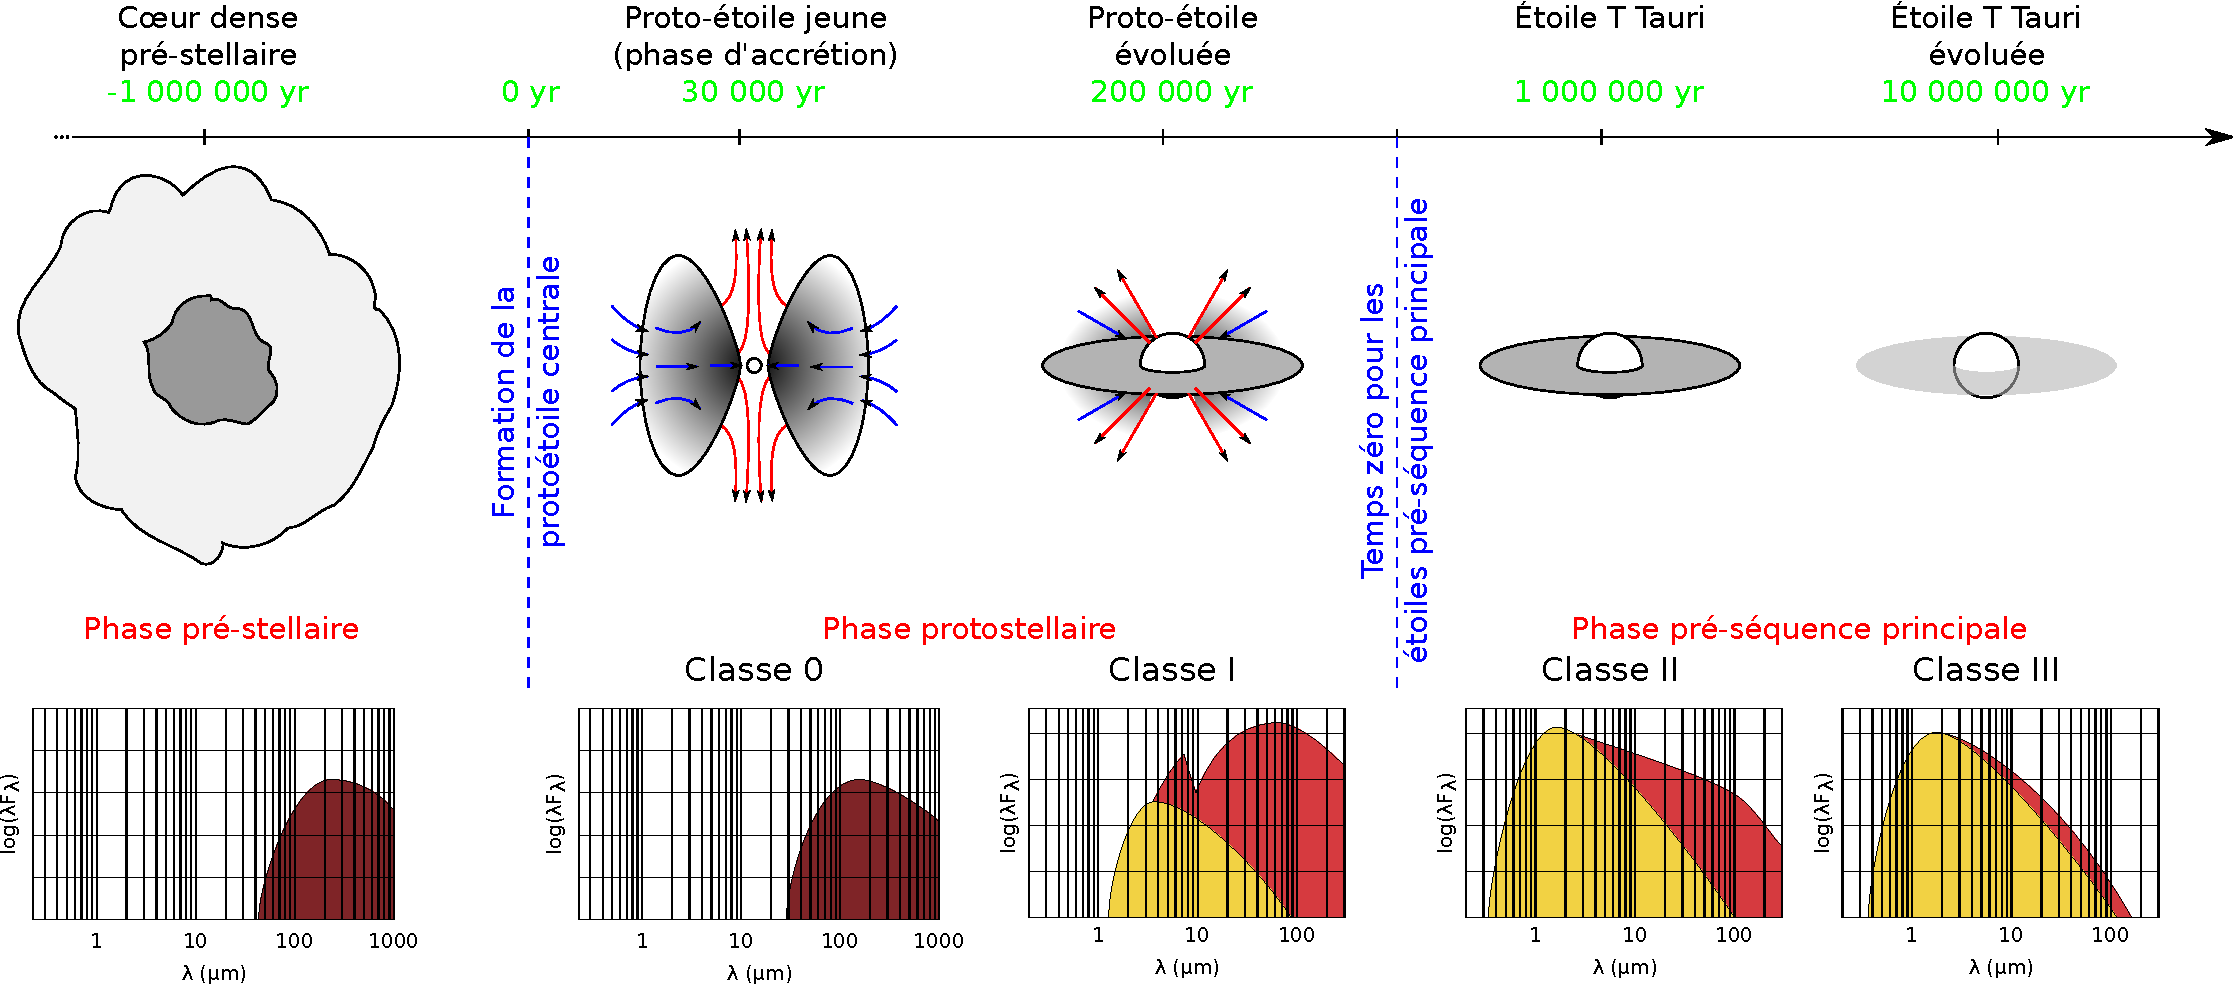
\includegraphics[width=\linewidth]{figure/star_formation.pdf}
\caption[Stades de formation d'une étoile]{Classification empirique des différents stades de formation des étoiles de faible
masse, du cœur dense pré-stellaire à la classe III. Schéma basé sur \citep{andre2002initial}. }\label{fig:star_formation}
\end{figure}


\section{Les disques protoplanétaires}
\subsection{Formation et évolution}
Durant les différentes phases de formation de l'étoile, alors même que le disque de gaz et de poussière se dissipe a lieu la formation des planètes. 

À mesure que le nuage s'effondre sur lui-même, et afin de satisfaire à la conservation du moment cinétique, ce dernier voit sa rotation accélérer, même si la rotation du nuage moléculaire était infime au départ. C'est ainsi que le disque d'accrétion, résultat de l'effondrement du nuage de gaz, est en rotation. L'effondrement d'un nuage moléculaire s'effectuant sur plusieurs ordres de grandeur (en distance), l'accélération de la rotation est d'autant plus grande.

Initialement, il est hautement improbable que le moment cinétique du nuage soit parfaitement nul. C'est ainsi que même si sa rotation est imperceptible lors des premiers stades de son effondrement gravitationnel, le disque d'accrétion fini toujours en rotation. 

\subsection{Évolution hydrodynamique du disque}
\begin{figure}[htbp]
\centering
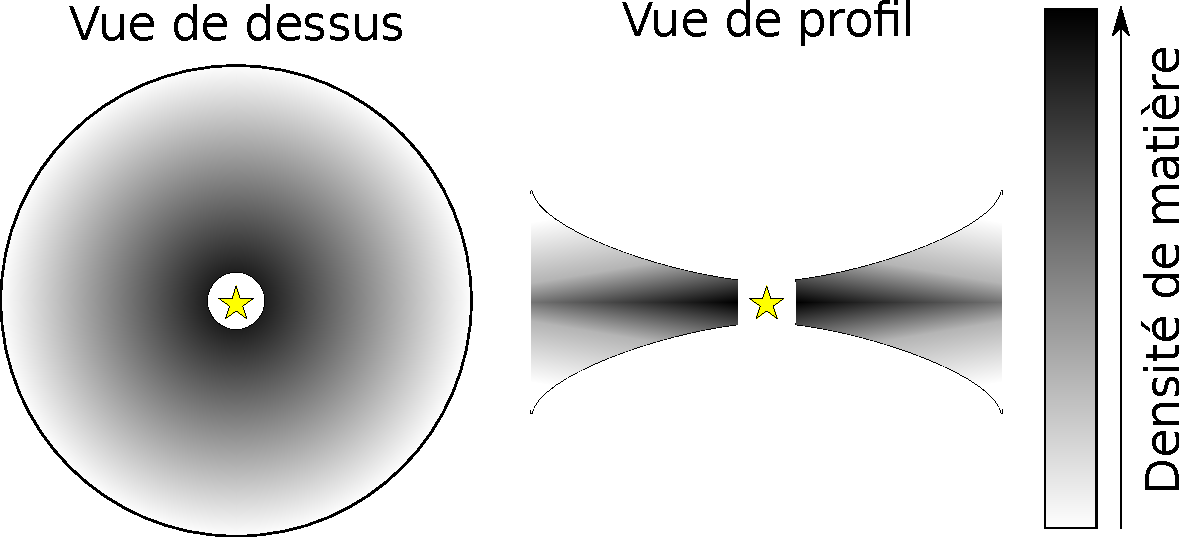
\includegraphics[width=0.6\linewidth]{figure/disk_scheme.pdf}
\caption[Vue de face et de profil d'un disque de gaz.]{Représentation de la répartition radiale et azimutale
de gaz dans un disque protoplanétaire.}\label{fig:disk_scheme}
\end{figure}

Avant de considérer l'évolution d'un disque, il est important de regarder sa masse par rapport à la masse de l'étoile centrale. En effet, si la masse du disque est de l'ordre de la masse de l'étoile, alors des instabilités se développent et on ne peut plus négliger l'autogravité du disque. 

Le \gras{paramètre de Toomre} $Q$, défini par \citep{toomre1964gravitational, goldreich1965gravitational}:
\begin{align}
Q &= \frac{\kappa c_{s}}{\pi G \Sigma}
\end{align}
est un indicateur de la stabilité du disque par rapport à l'auto-gravité. $\kappa$ est la fréquence épicyclique, $c_s$ la vitesse du son, $G$ la constante de gravitation universelle et $\Sigma$ la densité de surface. 

Dans ce paramètre, $\pi G \Sigma$ représente la masse du disque. La vitesse du son $c_{s}$ est liée à la pression thermique ; la \gras[fréquence!epicyclique@épicyclique]{fréquence épicyclique} $\kappa$ détermine quant à elle la force du cisaillement dans le disque.

\bigskip

Si $Q<1$ alors le gaz est instable gravitationnellement et il commence à s'effondrer sur lui-même et former des sur-densités à condition que le temps de refroidissement soit inférieur à 3 fois la période orbitale ($\tau_c \lesssim 3 \Omega^{-1}$) \citep{gammie2001nonlinear}.
Si $Q>1$, le disque est stable.

À partir du paramètre $Q$, on peut dériver une condition sur le rapport de masse entre étoile et disque pour que l'auto-gravité soit négligeable, ce qui donne \citep{gammie2001nonlinear} : 
\begin{align}
\frac{M_\text{d}}{M_\star} &\lesssim \frac{H}{R}
\end{align}
où $M_\text{d}$ et $M_\star$ sont respectivement la masse du disque et de l'étoile. $H$ est l'échelle de hauteur du disque et $R$ la distance par rapport à l'étoile.

Nous ne considérerons que des disques dont la masse $M_\text{d}$ est faible devant la masse de l'étoile $M_\star$. Si tel n'était pas le cas, le temps pour que le disque perde suffisamment de masse pour se retrouver dans le cas qui nous intéresse sera court devant la vie du disque et le temps de formation planétaire. Étant donné qu'on ne s'intéresse qu'aux derniers stades de la formation planétaire, à savoir quand les embryons planétaires ont une masse de l'ordre du dixième de masse terrestre au minimum, il est raisonnable de penser que le disque sera dans un stade peu dense où l'approximation $Q>1$ sera valable.

Dans un tel cas, c'est le potentiel gravitationnel de l'étoile qui domine la dynamique du gaz. En négligeant l'effet de la pression de ce dernier, on peut donc écrire la vitesse angulaire du gaz comme étant égale à la vitesse angulaire képlerienne : 
\begin{align}
\Omega &= \sqrt{\frac{GM_\star}{R^3}}
\end{align}
où $G$ est la constante de gravitation, et $R$ la distance à l'étoile. Dans la pratique, il est à noter que la vitesse est légèrement sous-képlerienne à cause de la pression du gaz. 

\bigskip

Il existe une force de cisaillement entre deux anneaux de gaz concentriques, dûs à leur différence de vitesse. Cette différence de vitesse génère des frottements à cause de la viscosité du disque $\nu$ (dont nous parlerons plus en détail plus loin \refsec{sec:viscosite}) qui chauffe le gaz en lui faisant perdre de l'énergie. En conséquence, une partie de l'énergie gravitationnelle du gaz est convertie en chaleur, qui est ensuite évacuée par le rayonnement de corps noir du gaz. 

\bigskip

La première conséquence est qu'un terme visqueux va apparaître dans l'équation de l'énergie, comme nous le verrons par la suite. 

La deuxième conséquence, c'est que le gaz perd de l'énergie, et donc dérive lentement vers l'étoile centrale qui accrète petit à petit le gaz du disque. 

On définit donc une vitesse de dérive négative $\vect{v_d} = v_r \hat{e}_r$, orientée vers l'étoile, qui entraine petit à petit le gaz du disque (avec $v_r$ négatif).

Dans la suite, nous allons nous intéresser à la conservation de différentes quantités, que ce soit la masse ou le moment cinétique. Pour cela nous allons définir un anneau de référence, portion du disque sur laquelle nous allons faire le bilan. Le but est ici de présenter d'où viennent les équations et plus précisément d'où viennent les termes des équations. 

\bigskip

Afin de décrire l'évolution hydrodynamique du disque de gaz, nous allons utiliser successivement la \textbf{conservation de la masse}, et la \textbf{conservation du moment cinétique.}. Les démonstrations qui vont suivre ont été déjà faites de nombreuses fois, notamment par \citep{pringle1981accretion}.

\subsubsection{Structure verticale du disque}
On s'intéresse à la répartition de masse verticalement dans le disque. Afin de définir les quantités importantes qui s'y rapportent, nous allons écrire l'équation de l'équilibre hydrostatique. On a alors :
\begin{align}
\inv{\rho}\dpd{P}{z} &= \vect{g}.\hat{e}_z\\
&= \left(-\frac{GM}{R^3}\hat{e}_r\right).\hat{e}_z
\end{align}

$\vect{g}$ est orienté vers l'étoile centrale, selon la direction $r$ (en sphérique). En projetant sur l'axe $z$ pour effectuer le produit scalaire, et en faisant l'approximation que $r\sim a$ on obtient alors :
\begin{align}
\inv{\rho}\dpd{P}{z} &= -\Omega^2 z
\end{align}

En considérant un disque isotherme selon $z$ et d'après la loi des gaz parfaits
\begin{align}
P &= \frac{\rho k_B T}{\mu m_H}
\end{align}
il vient
\begin{align}
\dpd{\rho}{z} &= -\frac{\mu m_H\Omega^2}{k_B T}\rho z
\end{align}

On obtient alors :
\begin{align}
\rho(z) &= \rho_0\exp\left(-\frac{z^2}{2H^2}\right)
\end{align}
où $\rho_0$ est la densité volumique du disque de gaz dans le plan médian et $H$ l'échelle de hauteur du disque est définie par (dans la limite isotherme) : 
\begin{align}
H &= \sqrt{\frac{k_B T}{\Omega^2 \mu m_H}}
\end{align}

\bigskip

Sachant que la vitesse du son, définie par :
\begin{align}
{c_s}^2=\frac{P}{\rho} &= \frac{k_B T}{\mu m_H}
\end{align}
dans le cas d'un gaz parfait, on peut alors écrire la relation suivante entre l'échelle de hauteur et la vitesse du son : 
\begin{align}
c_s &= H\Omega
\end{align}

\bigskip

On considèrera dans la suite les quantités moyennées selon $z$, et en particulier on défini la densité de surface $\Sigma$ de la façon suivante : 
\begin{align}
\Sigma &= \int_{-\infty}^{+\infty} \rho \dif z\nonumber\\
&=\rho_0 \int_{-\infty}^{+\infty}  \exp\left(-\frac{z^2}{2H^2}\right)\dif z\nonumber\\
\Sigma &= \sqrt{2\pi}\rho_0 H\label{eq:surface-to-volume}
\end{align}

% fromang & nelson 2006 donnent une formule, après l'équation (20), mais elle ne correspond pas à ça, peut-être lié à un truc magnétique ou je sais pas quoi

\subsubsection{Bilan de masse}
\begin{figure}[htbp]
\centering
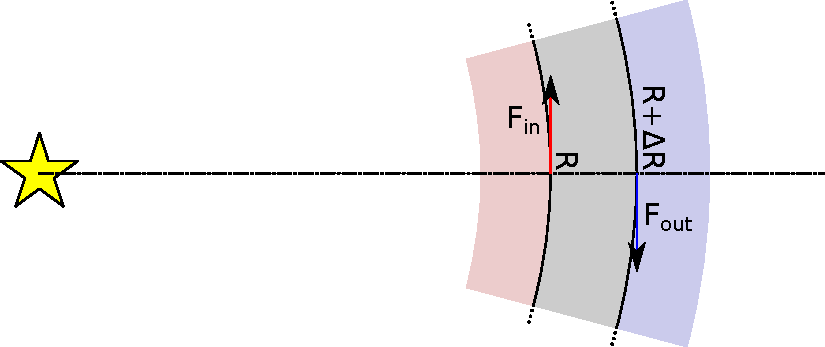
\includegraphics[width=0.7\linewidth]{figure/disk_ring.pdf}
\caption[Bilan de moment cinétique d'un anneau d'épaisseur $\Delta R$.]{Représentation d'un anneau de largeur $\Delta R$ et du
bilan de moment cinétique de ce dernier.}\label{fig:disk_ring}
\end{figure}

On cherche dans un premier temps à faire le bilan de masse de l'anneau considéré. Sa masse s'écrit :
\begin{align}
m_a &= 2\pi R \Delta R \Sigma(R)\label{eq:m_a}
\end{align}

\bigskip

Soit $v_r\hat{e}_r$ la vitesse radiale du gaz (avec $v_r<0$ dans notre cas). Cette vitesse est responsable d'un certain taux d'accrétion du gaz du disque sur l'étoile centrale. On cherche maintenant à modéliser cette accrétion pour le bilan de moment cinétique sur l'anneau.

Pour cela, on cherche à exprimer la variation de masse de l'anneau, ainsi que le moment cinétique emporté par cette variation de masse. 

Au bord interne $R$, par unité de temps, la masse entrant ou sortant de l'anneau peut-être exprimée comme un flux :
\begin{align}
\dif F_M &= \Sigma \cdot 2\pi r \cdot \left( -\vect{v_r} \cdot \vect{\dif S} \right)
\end{align}
En effet, en multipliant la circonférence de l'anneau par la vitesse, on obtient une sorte de surface par unité de temps qui représente ce qui sort de la frontière virtuelle représentée par l'anneau en $r=R$. 

Le flux de matière doit être négatif si la masse sort de l'anneau. Les éléments de surface étant orientés vers l'extérieur, un vecteur vitesse colinéaire à $\vect{\dif S}$ implique que la matière sort de l'anneau. Ceci explique la présence du signe négatif dans l'expression du flux de matière.

On a ainsi aux deux bords de l'anneau :
\begin{subequations}
\begin{align}
\dif F_M(R) &= \Sigma(R) \cdot 2\pi R \cdot v_r(R)\\
\dif F_M(R+\Delta R) &= - 2\pi (R+\Delta R) \cdot v_r(R+\Delta R) \cdot \Sigma(R+\Delta R)
\end{align}\label{eq:dif_F_M}
\end{subequations}
$v_r$ étant négatif, on a bien une perte de masse en $r=R$ et un gain de masse en $r=R+\Delta R$.

La conservation de la masse implique alors que la dérivée temporelle de la masse de l'anneau est égale au flux de masse à travers sa surface. On a ainsi : 
\begin{align*}
\dpd{}{t}\left(2\pi R \Delta R \Sigma(R)\right) &= \dif F_M(R) + \dif F_M(R+\Delta R)
\end{align*}

En faisant tendre l'épaisseur $\Delta R$ de l'anneau vers 0, on obtient alors :
\begin{important}
\begin{align}
\dpd{\Sigma}{t} + \inv{R}\dpd{}{r}\left(R v_r \Sigma\right)&=0\label{eq:conservation_masse}
\end{align}
\end{important}

\subsubsection{Bilan de moment cinétique/angulaire}
On fait maintenant un bilan des variations de moment cinétique pour l'anneau de gaz. Pour cela on dit que la variation de moment cinétique (que l'on écrit en dérivant $J_a(t)$) est égale aux variations de moment cinétiques induites aux bords de l'anneau par échange de masse à laquelle s'ajoute la différence entre les deux couples visqueux qui s'appliquent au bord externe et interne. Ce qui donne : 
\begin{align}
\dod{J_a}{t} &= \dif J(R+\Delta R) + \dif J(R) + \Gamma_\text{out} - \Gamma_\text{in}\label{eq:cons_J_a}
\end{align}

Le moment cinétique de l'anneau est défini par :
\begin{align}
\vect{J_a} &= \vect{R} \wedge (m_a\vect{v(R)}) \nonumber\\
\vect{J_a} &= 2\pi R^3 \Delta R \Sigma(R)\Omega(R)\hat{e}_z\label{eq:J_a}
\end{align}
où $\Sigma$ et $\Omega$ sont la densité de surface et la vitesse angulaire du gaz à la position $R$ dans le disque.

Le flux de moment cinétique est simplement défini comme la quantité de moment cinétique emportée ou apportée par le flux de masse défini précédemment \refeq{eq:dif_F_M} :
\begin{subequations}
\begin{align}
\dif J(R) &= 2\pi v_r(R) \Sigma(R)\cdot R^3\Omega(R)\hat{e}_z\label{eq:dJ_in}\\
\dif J(R+\Delta R) &= -2\pi v_r(R+\Delta R) \Sigma(R+\Delta R)\cdot \left(R+\Delta R\right)^3\Omega(R+\Delta R)\hat{e}_z\label{eq:dJ_out}
\end{align}\label{eq:dJ}
\end{subequations}

\bigskip

À ceci s'ajoute la variation de moment cinétique induite par la friction entre anneaux concentriques, en d'autres termes, dus à la viscosité du disque. Cette variation de moment cinétique est représentée sous la forme d'un couple exercé par les anneaux internes et externes à celui considéré. 

La force visqueuse par unité de longueur est définie par :
\begin{align}
\dif F_\text{vis} &= \nu \Sigma A = \nu \Sigma r \dod{\Omega}{r}
\end{align}
où $A=r \dod{\Omega}{r}$ est le taux de cisaillement.

La force visqueuse induite par les anneaux entourant l'anneau considéré est alors : 
\begin{subequations}
\begin{align}
\vect{F_\text{in}}(R)&= 2\pi\nu \Sigma R^2 \dod{\Omega}{r}(R) \hat{e}_\theta\\
\vect{F_\text{out}}(R+\Delta R)&= 2\pi\nu \Sigma (R+\Delta R)^2 \dod{\Omega}{r}(R+\Delta R) \cdot \hat{e}_\theta
\end{align}
\end{subequations}
L'anneau interne tournant plus vite, la force est dirigée dans le sens de rotation $\hat{e}_\theta$. À l'inverse, l'anneau externe tourne moins vite, il tend à freiner l'anneau de référence et s'oppose à son mouvement. La force est donc opposée au sens de rotation.

\bigskip

Ainsi, le couple $\vect{\Gamma}=\vect{r}\wedge\vect{F}$ issu de chacun des anneaux entourant celui de référence s'écrit :
\begin{subequations}
\begin{align}
\vect{\Gamma_\text{in}} &= 2\pi\nu \Sigma R^3 \dod{\Omega}{r}(R) \hat{e}_z\label{eq:G_in}\\
\vect{\Gamma_\text{out}} &= 2\pi\nu \Sigma (R+\Delta R)^3 \dod{\Omega}{r}(R+\Delta R) \hat{e}_z\label{eq:G_out}
\end{align}\label{eq:J_torques}
\end{subequations}

\bigskip

En utilisant \refeq{eq:J_a}, \refeq{eq:dJ}, \refeq{eq:J_torques}, dans \refeq{eq:cons_J_a} il vient alors :
\begin{align}
\dpd{\Sigma}{t} &= \inv{r}\dpd{}{r}\left\{\inv{\dpd{}{r}\left(r^2\Omega\right)} \dpd{}{r}\left[\nu \Sigma r^3 \left(-\dod{\Omega}{r}\right)\right]\right\}
\end{align}

Dans le cas d'un disque képlerien ($\Omega = \sqrt{\frac{GM}{r^3}}$) on obtient finalement :
\begin{important}
\begin{align}
\dpd{\Sigma}{t} &=\frac{3}{r}\dpd{}{r}\left[\sqrt{r} \dpd{}{r}\left(\nu \Sigma r^\sfrac{1}{2}\right)\right]
\end{align}
\end{important}

Le calcul détaillé est disponible \refsec{app:equation_angular_momentum}.

Cette équation a nécessité les approximations suivantes : 
\begin{enumerate}
\item On suppose que le potentiel gravitationnel est indépendant du temps ($\dod{\Omega}{t}=0$), c'est-à-dire que la masse de l'étoile est constante, l'accrétion ayant un effet négligeable.
\item On suppose que le mouvement du gaz est képlerien $\Omega=\sqrt{\frac{GM}{r^3}}$, ce qui n'est pas rigoureusement vrai, la pression du gaz rendant le mouvement légèrement sous-képlerien.
\end{enumerate}

\subsubsection{Temps de vie et dispersion du disque}\label{sec:dispersion}\index{dissipation du disque}

\begin{figure}[htbp]
\centering
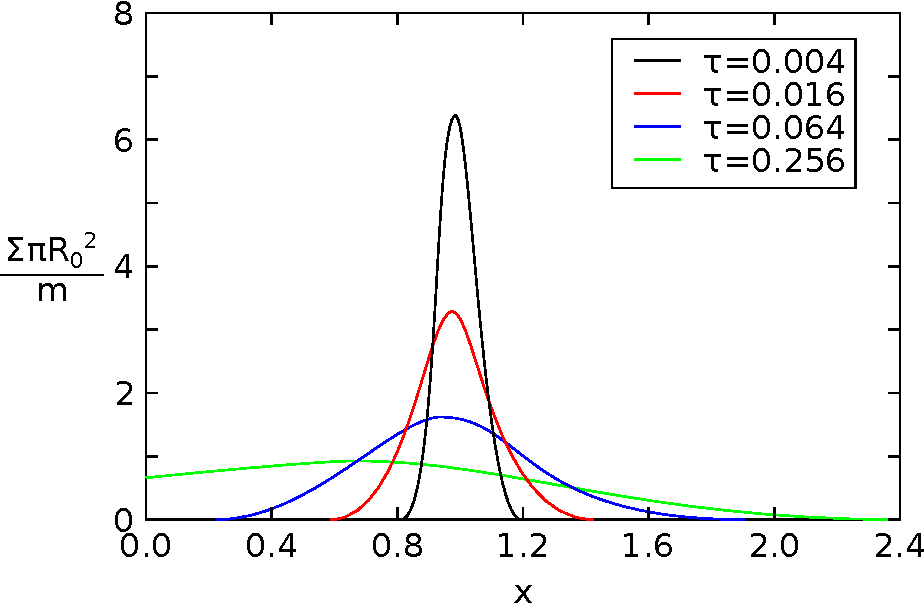
\includegraphics[width=0.65\linewidth]{figure/pringle_viscous_dissipation.pdf}
\caption[Évolution visqueuse d'un anneau de matière]{Évolution visqueuse d'un anneau de matière de masse $m$ et de rayon $R_0$.
La densité de surface est montrée comme une fonction de la longueur dédimensionnée $x=R/R_0$ et du temps adimensionné
$\tau=12\nu t / {R_0}^2$.}\label{fig:pringle_viscous_dissipation}
\end{figure}

Cette équation permet de modéliser l'évolution visqueuse d'un disque au cours du temps. \reffig{fig:pringle_viscous_dissipation}, tirée de \cite{pringle1981accretion} et recalculée illustre l'évolution visqueuse d'un anneau de matière de masse $m$ dans des unités adimensionnées de distance et de temps.

\bigskip

On situe généralement le temps de vie d'un disque protoplanétaire autour de quelques millions d'années. Cette information est obtenue de plusieurs études de d'amas d'étoiles d'âges différents dans lesquelles on mesure le taux d'étoiles possédant un excès infrarouge (signe de présence d'un disque) \citep{williams2011protoplanetary}. 70\% à 80\% des étoiles jeunes ($t<1\unit{Myr}$) possèdent un disque \citep{winston2007combined, gutermuth2008spitzer}, 40 à 50\% des étoiles dans des amas d'âge compris entre 2 et 3 millions d'années en possèdent un \citep{lada2006spitzer, sung2009spitzer} tandis que moins de 20\% des étoiles dans des amas d'environ 5 millions d'années ont un disque \citep{currie2009last}. 

Par la rareté des disques en train de se dissiper, les observations suggèrent aussi que les disques se dissipent très rapidement, avec un temps de dispersion d'environ $10^5$ ans \citep{simon1995disk, wolk1996search}. La dissipation visqueuse n'explique alors pas comment le disque peut subsister pendant plusieurs millions d'années, mais se dissiper complètement en \nombre{500 000} ans. \cite{clarke2001dispersal} ont montré qu'il était possible d'expliquer ce comportement à deux temps caractéristiques à l'aide de la photo-évaporation. 

\begin{figure}[htbp]
\centering
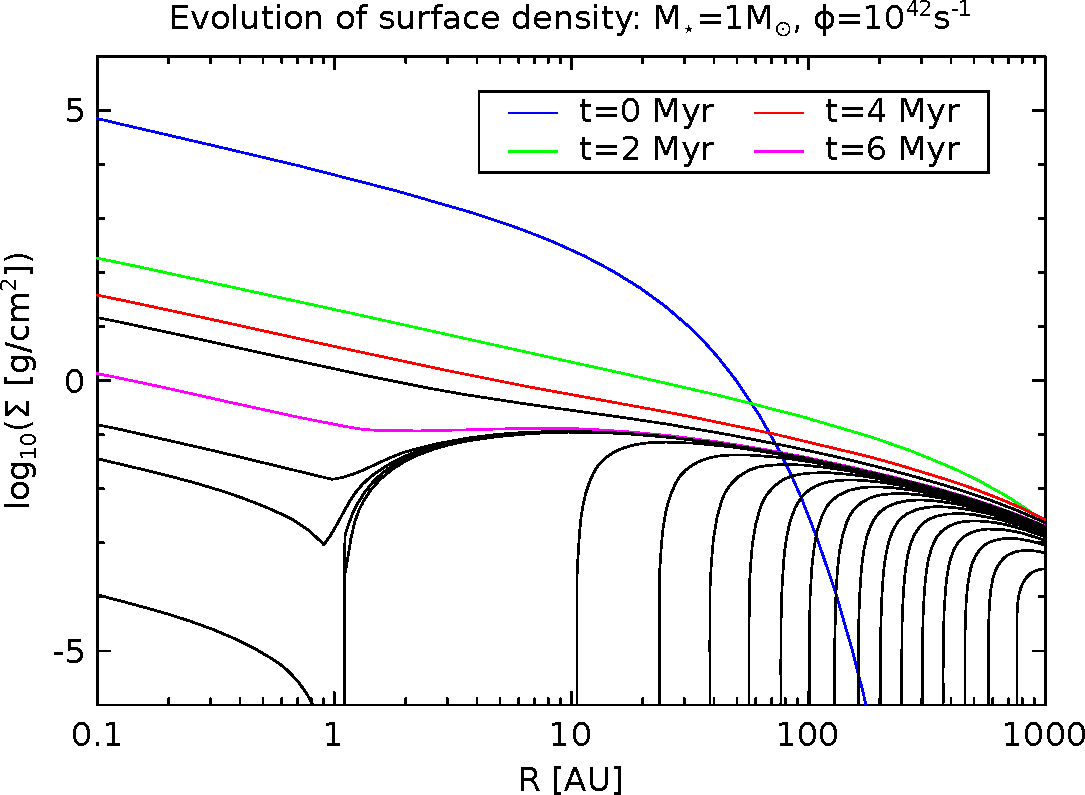
\includegraphics[width=0.65\linewidth]{figure/disk_dispersion.pdf}
\caption[Dissipation du disque]{Évolution de la densité de surface en fonction du temps dans une simulation qui modélise la
dissipation du disque protoplanétaire par évolution visqueuse et photo-évaporation. À $t=6.20\unit{Myr}$ le disque est
totalement dissipé. Figure adaptée de \cite{alexander2006photoevaporation}.}\label{fig:disk_dispersion}
\end{figure}

Le principe de la \gras{photo-évaporation} est que le rayonnement de l'étoile permet de dissocier le dihydrogène ainsi que de fournir de l'énergie cinétique aux atomes du gaz. À partir d'un rayon dit \og rayon gravitationnel\fg $r_g$ qui représente la distance à partir de laquelle l'énergie fournie par les photons de l'étoile devient suffisante pour contrebalancer les effets de sa gravité, la photo-évaporation permet d'évaporer une partie du gaz superficiel du disque. Le disque va alors se creuser jusqu'à séparer le disque en deux. Les parties internes du disques ne sont alors plus alimentées par les parties externes. Des simulations montrent que les parties externes se dispersent rapidement une fois les parties internes accrétées \citep{alexander2006photoevaporation}. \reffig{fig:disk_dispersion} montre l'évolution du profil radial de densité en fonction du temps en présence de l'évolution visqueuse et de la photo-évaporation.

La photo-évaporation est aussi possible par l'irradiation d'étoiles massives (étoiles OB) dans le voisinage du disque \citep{adams2004photoevaporation}.

\subsection{Profil de température}
Du point de vue de la température, il y a principalement deux types de disques : 
\begin{itemize}
\item les \gras[chauffage visqueux]{disques actifs} : la source de température est le disque lui-même, qui par \gras{chauffage visqueux} (frottements) va convertir de l'énergie gravitationnelle en chaleur ;
\item les \gras[irradiation]{disques passifs} : la source de chaleur/température est l'étoile centrale qui éclaire le disque. 
\end{itemize}

Un disque peut à la fois être actif et passif, mais généralement on essaie d'approximer, de considérer que l'un est négligeable devant l'autre. De plus, un disque aura des zones actives et des zones passives, c'est-à-dire que certaines zones seront principalement chauffées par la viscosité alors que d'autres le seront par l'\gras[irradiation]{irradiation de l'étoile}.

\bigskip

Afin de déterminer le profil de température, il faut écrire l'équation de conservation de l'énergie, qui va tenir compte de tous les termes source et toutes les pertes, par unité de surface.

On a tout d'abord les pertes par rayonnement de corps noir. Ensuite, il y a les termes sources. Pour un disque actif, le terme source est le chauffage visqueux. Pour un disque passif, c'est l'irradiation de l'étoile \citep{chiang1997spectral}. Dans notre cas, il y a un terme dû à l'enveloppe du disque, un dû à l'irradiation de l'étoile centrale, et enfin un dernier dû au chauffage visqueux.


\begin{figure}[htbp]
\centering
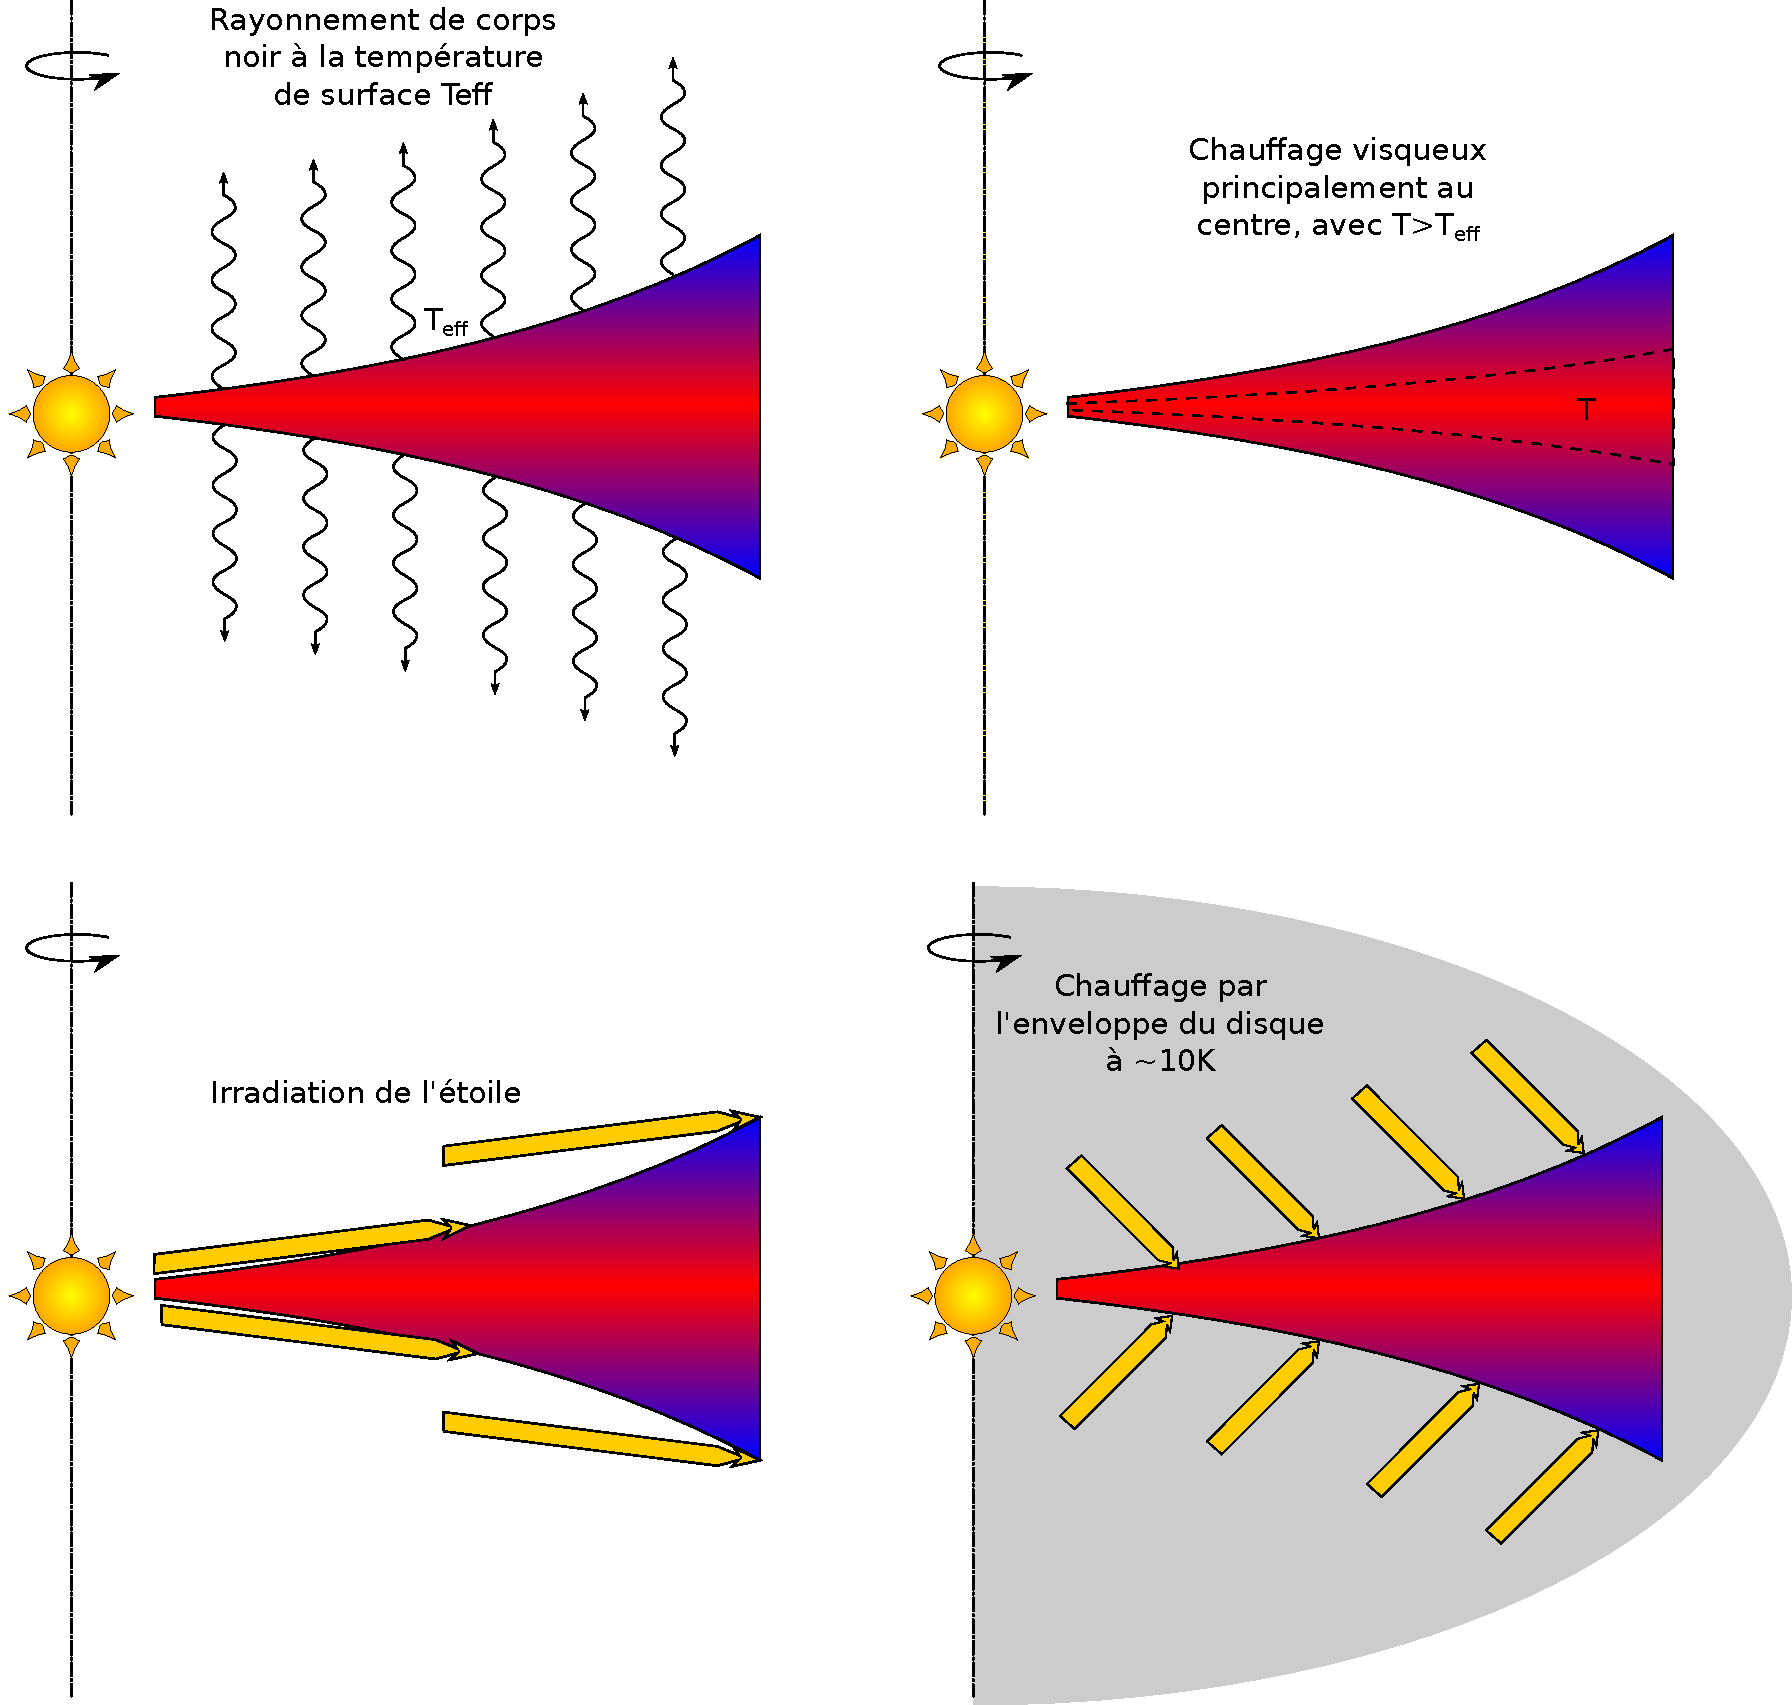
\includegraphics[width=0.65\linewidth]{figure/disk_energy.pdf}
\caption[Bilan énergétique d'un disque.]{Représentation du bilan thermique d'un disque}\label{fig:energy_equilibrium}
\end{figure}

\subsubsection{Refroidissement radiatif}
Par toute la surface du disque, qui est à une température $T_\text{eff}$ en surface, on a des pertes par rayonnement de corps noir : 
\begin{align}
P_\text{cn} &= - 2\sigma {T_\text{eff}}^4
\end{align}
où $\sigma$ est la constante de Stefan-Boltzmann. Ces dernières doivent être multiplié par deux, en effet, il y a des pertes par rayonnements des deux cotés du disque à une position donnée. 

\bigskip

$T_\text{eff}$ est une estimation de la température effective du disque à sa surface \cite{hubeny1990vertical} : 
\begin{subequations}
\begin{align}
{T_\text{eff}}^4 &= \frac{T^4}{\tau_\text{eff}}
\intertext{avec}
\tau_\text{eff} &= \frac{3}{8}\tau + \frac{\sqrt{3}}{4} + \inv{4\tau}
\end{align}
\end{subequations}
où $\tau=\kappa\Sigma/2$ est la profondeur optique verticale moyenne, $\kappa$ étant l'opacité du disque (l'opacité sera détaillée dans \refsec{sec:opacity}).

Cette température effective est le résultat d'un transfert de rayonnement depuis le cœur du disque, à une température $T$ qui se refroidit, et chauffe les différentes couches successives jusqu'à atteindre le bord du disque. Il résulte alors une température $T_\text{eff}$ plus faible que la température dans le plan du disque. 

\subsubsection{Chauffage par l'enveloppe}
\begin{figure}[htbp]
\centering
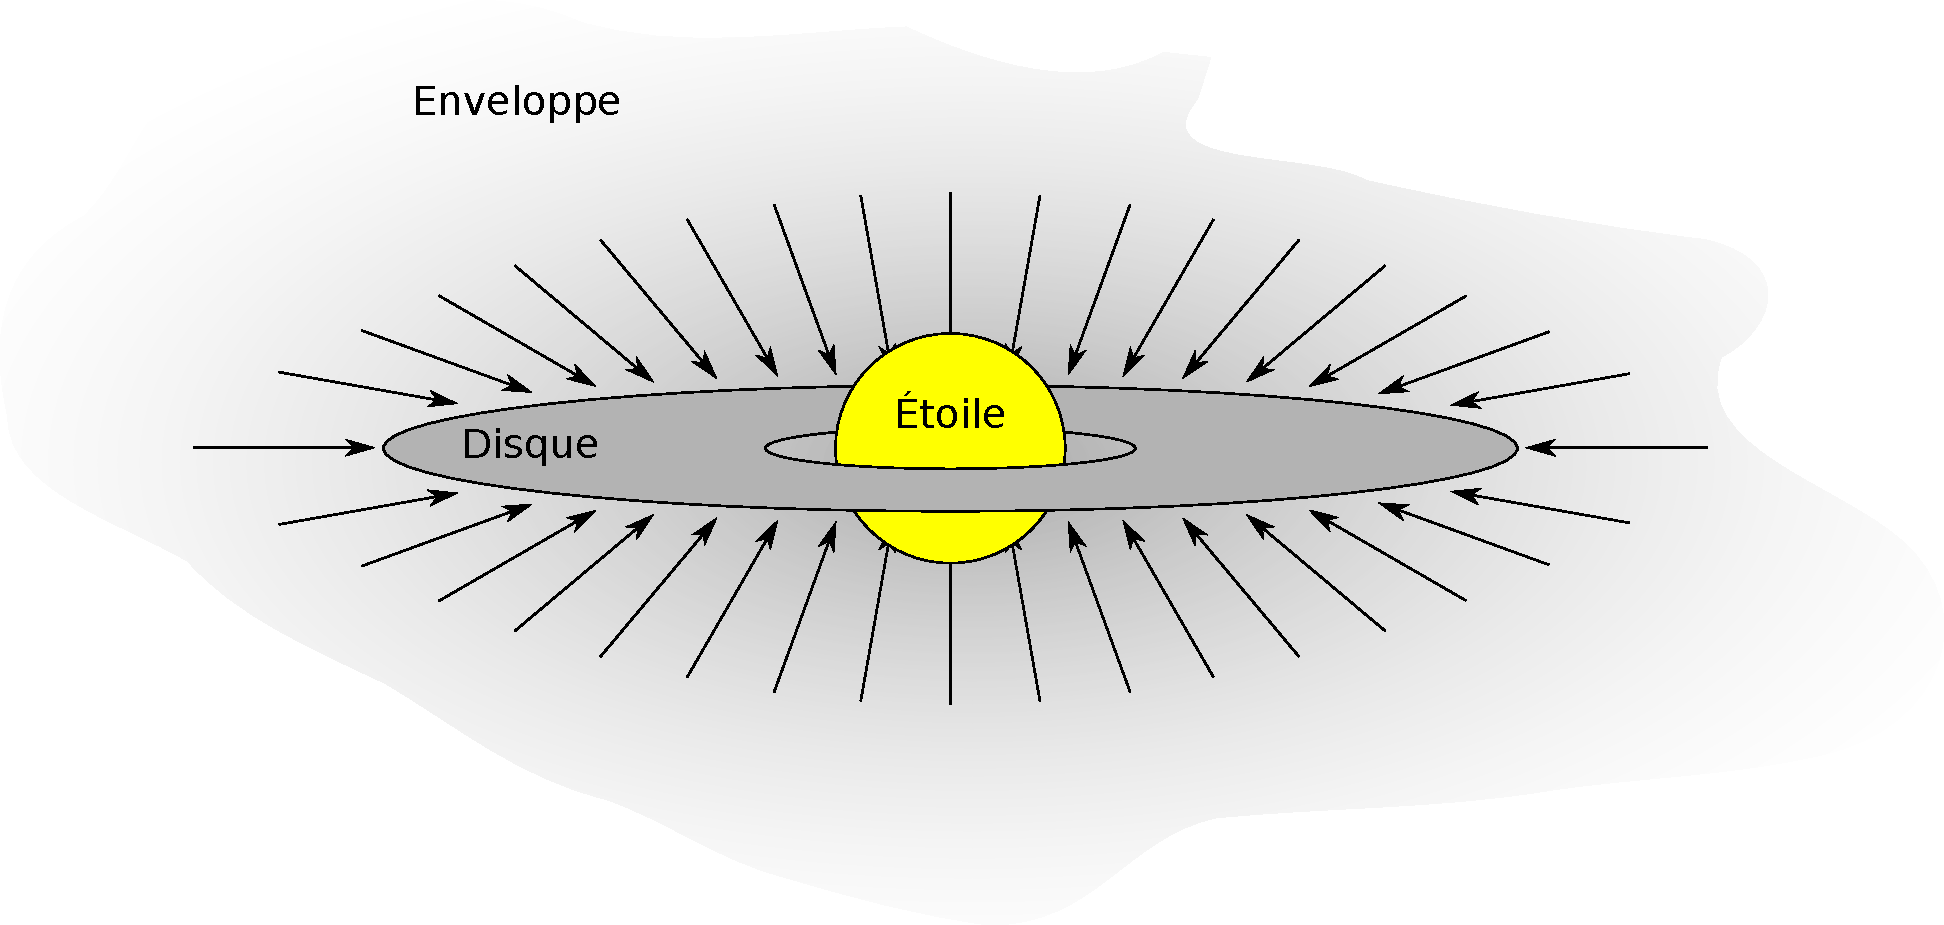
\includegraphics[width=0.65\linewidth]{figure/disk_envelope.pdf}
\caption[Chauffage du disque par l'enveloppe]{Représentation de l'effondrement d'un nuage moléculaire et des différentes parties
qui composent le système en effondrement.}\label{fig:envelope}
\end{figure}
L'enveloppe \reffig{fig:envelope} provient de l'effondrement continu du nuage moléculaire. C'est un reste diffus qui alimente continuellement le disque en matière. Mais cette enveloppe, qui possède une température que l'on fixe ici à $T_\text{en} = 10\unit{K}$ contribue aussi au bilan d'énergie du disque en apportant la contribution uniforme suivante :
\begin{align}
C_\text{en} &= 2 \sigma {T_\text{en}}^4
\end{align}

La température de l'enveloppe étant très faible, cette dernière ne contribue que dans les parties externes du disque, là où la densité de surface du gaz est très faible, rendant du même coup le chauffage visqueux extrêmement ténu lui aussi.

\subsubsection{Chauffage par l'étoile}\label{sec:irradiation}\index{irradiation}
La surface du disque reçoit de la lumière de l'étoile centrale. Soit $R_\star$, $L_\star$ respectivement le rayon et la luminosité de l'étoile. Soit $\varepsilon$ l'albédo du disque, que l'on choisi typiquement égal à $0.5$  \citep{menou2004low}. 

Le flux incident est alors \citep[eq. (7)]{menou2004low} : 
\begin{align}
F_\text{irr} &= \frac{L_\star(1-\varepsilon)}{4\pi r^2} \alpha
\end{align}
où $\alpha$ (avec $\alpha\ll 1$) représente l'angle entre les rayons incidents et la surface du disque. 

D'après notamment \cite[eq. (5)]{chiang1997spectral}, cet angle peut être écrit comme : 
\begin{align}
\alpha &= 0.4 \frac{R_\star}{r} + r \dod{}{r}\left(\frac{H}{r}\right)
\end{align}

On note que dans cette expression, le premier terme illustre le fait que l'étoile n'est pas ponctuelle, et que ceci a un effet sur l'irradiation dès que l'on s'approche de cette dernière. Le deuxième terme représente la surface du disque qui intercepte le rayonnement incident, et qui est fonction de la variation d'échelle de hauteur du disque (plus le disque est évasé, et plus la paroi qui intercepte le rayonnement est abrupte). 

Il vient enfin, en exprimant la luminosité de l'étoile en fonction de sa température et de son rayon, l'expression suivante :
\begin{align}
C_\text{irr} &= 2 \sigma {T_\star}^4 \frac{{R_\star}^2}{r^2} (1-\varepsilon) * \left[0.4 \frac{R_\star}{r} + r \dod{}{r}\left(\frac{H}{r}\right)\right]
\end{align}

Il faut cependant noter qu'une approximation implicite a été faite, c'est de dire que $h_p\sim h$, où $h_p$ est la position verticale dans le disque où les photons stellaires sont absorbés. En effet, l'absorption des photons ne dépend pas simplement de la densité, mais aussi de l'opacité du disque aux photons stellaires, qui dépend de la composition du disque.

Dans le cadre d'un disque optiquement épais, il devient possible de considérer $h_p \sim h$.

%non ponctualité de l'étoile : Chiang & Goldreich, 1997, ApJ, 490, 368
%expression de l'angle notammenet : dullemond 2000
%autres expressions : menou & goodman 2004

\subsubsection{Chauffage visqueux}\index{chauffage visqueux}
On considère un fluide incompressible. Il peut paraître étonnant de considérer un disque de gaz comme étant un fluide incompressible. Mais en fait l'aspect compressible va surtout se manifester lors de la mise à l'équilibre, générant des ondes de chocs par exemple. Mais une fois le disque stabilisé tout se passe comme si on avait un fluide incompressible. C'est matérialisé par le fait que la vitesse dans le disque est considérée comme inférieure à la vitesse du son dans le milieu $c_s$, au delà de laquelle on aura des ondes des choc ayant une incidence sur le bilan thermique. Ainsi donc, en considérant un fluide incompressible, on peut partir de l'expression de la variation d'énergie cinétique (qui est l'inverse du chauffage, les pertes cinétiques étant converties en chaleur par la viscosité) \citep[(16.3)]{landau1989mecanique} : 
\begin{align}
\dpd{E_c}{t} &= - \frac{1}{2}\int \eta(T_{ik})^2\dif V\\
T_{ik} &= \left(\dpd{v_i}{x_k} + \dpd{v_k}{x_i}\right)\nonumber
\end{align}
où $\eta = \rho\nu$ est la viscosité dynamique\footnote{$\nu$ étant la viscosité cinématique et $\rho$ la densité volumique de gaz.}

À partir de \citep[(15.8) et (15.17)]{landau1989mecanique}, on extrait de manière assez directe l'expression du tenseur $T_{ik}$ en coordonnées cylindriques : 
\begin{align}
T_{rr} &= 2\dpd{v_r}{r}, & T_{r\varphi} &= \left(\inv{r} \dpd{v_r}{\varphi} + \dpd{v_\varphi}{r} - \frac{v_\varphi}{r}\right),\nonumber\\
T_{\varphi\varphi} &= 2 \left(\inv{r} \dpd{v_\varphi}{\varphi} + \frac{v_r}{r}\right), & T_{\varphi z} &= \left(\dpd{v_\varphi}{z} + \inv{r}\dpd{v_z}{\varphi}\right),\\
T_{zz} &= 2\dpd{v_z}{z}, & T_{rz} &= \left(\dpd{v_z}{r} + \dpd{v_r}{z}\right).\nonumber
\end{align}
sachant que le tenseur est symétrique en statique, ce qui donne : 
\begin{align}
T_{ik} &= \begin{pmatrix}
T_{rr} & T_{r\varphi} & T_{rz}\\
T_{r\varphi} & T_{rr} & T_{\varphi z}\\
T_{rz} & T_{\varphi z} & T_{zz}
\end{pmatrix}
\end{align}

À partir de ces expressions, nous allons procéder à quelques simplifications, moyennant quelques approximations : 
\begin{itemize}
\item On considère tout d'abord que $v_z=0$ en invoquant le fait que le disque est à l'équilibre hydrostatique verticalement. 

\item Ensuite, on néglige tous les termes en $\pd{}{\varphi}$ car le disque est axisymétrique. 

\item On néglige enfin tous les termes en $v_r$ devant les termes en $v_\varphi$ étant donné que la vitesse de dérive (liée à l'accrétion) est beaucoup plus petite que la vitesse de rotation due au mouvement képlerien. En effet, la vitesse de dérive est une conséquence des pertes d'énergie par frottement visqueux entre deux anneaux due à la différence de vitesse de leur mouvement képlerien.
\end{itemize}

Seul le terme $T_{r\varphi}$ reste :
\begin{align}
T_{r\varphi} &= \dpd{v_\varphi}{r} - \frac{v_\varphi}{r}\nonumber\\
\intertext{avec $v_\varphi=r\Omega$}
T_{r\varphi} &= r\dod{\Omega}{r}
\end{align}

Il vient alors :
\begin{align*}
\dpd{E_c}{t} &= - \frac{1}{2}\int \eta(T_{ik})^2\dif V\\
&= - \frac{1}{2}\int \eta\sum_{i=1}^3\sum_{j=1}^3 {T_{ij}}^2\dif V\\
&= - \frac{1}{2}\int \eta\left({T_{r\varphi}}^2+{T_{\varphi r}}^2\right)\dif V\\
\intertext{Le tenseur est symétrique, on a donc $T_{r\varphi} = T_{\varphi r}$}
&= - \frac{1}{2}\int \eta\left(2{T_{r\varphi}}^2\right)\dif V\\
&= - \iint \rho\nu \left(r\dod{\Omega}{r}\right)^2\dif S\dif z\\
\intertext{En utilisant une vitesse angulaire képlerienne $\Omega=\sqrt{\frac{GM}{r^3}}$ on obtient alors :}
&= - \int \Sigma\nu \left(-\frac{3}{2}\Omega\right)^2\dif S\\
\dpd{E_c}{t} &= - \frac{9}{4} \int \Sigma\nu \Omega^2\dif S
\end{align*}

La variation d'énergie cinétique est négative, cette perte est convertie en chaleur par chauffage visqueux. Le chauffage visqueux intégré sur toute la surface du disque peut ainsi être défini comme : 
\begin{align*}
C_\text{vis/tot} &= - \dpd{E_c}{t}
\end{align*}
de sorte qu'on peut écrire le chauffage visqueux par unité de surface comme étant égal à :
\begin{align}
C_\text{vis} &= \frac{9}{4} \nu\Sigma\Omega^2
\end{align}

\subsubsection{Bilan}
On cherche maintenant la température d'équilibre du disque, compte tenu de tous les termes rentrant dans l'équation bilan de l'énergie du disque. Il vient alors, en considérant le chauffage visqueux, l'irradiation de l'étoile centrale, le chauffage par l'enveloppe et les pertes par radiation à la surface du disque : 
\begin{align}
0 &= P_\text{cn} + C_\text{en} + C_\text{irr} + C_\text{vis}\nonumber\\
0 &= - 2\sigma \frac{T^4}{\frac{3}{8}\tau + \frac{\sqrt{3}}{4} + \inv{4\tau}} + 2 \sigma {T_\text{en}}^4 + 2 \sigma {T_\star}^4 \frac{{R_\star}^2}{r^2} (1-\varepsilon) * \left[0.4 \frac{R_\star}{r} + r \dod{}{r}\left(\frac{H}{r}\right)\right] + \frac{9}{4} \nu\Sigma\Omega^2\label{eq:equation_energie}
\end{align}

Dans la pratique, c'est une équation de l'on résout de manière numérique, par itération. En effet, beaucoup de paramètres dépendent de la température, alors même que c'est la variable que l'on recherche. 

Ce calcul est lui-même extrêmement dépendant de la définition que l'on choisi pour l'opacité $\kappa$ et de la dépendance de cette dernière en fonction de la température, la densité ou la pression. 

\subsection{La viscosité du disque}\label{sec:viscosite}\index{viscosité}% (Franck et al. 1992)
La viscosité moléculaire, viscosité généralement considérée quand on étudie la dynamique d'un fluide, peut être définie par : 
\begin{align}
\nu_m &\sim \lambda c_s
\end{align}
où $c_s$ est la vitesse du son dans le milieu et $\lambda$, libre parcours moyen dans le gaz avec une concentration de particule $n$ est :
\begin{align}
\lambda &= \inv{n\sigma_\text{mol}}
\end{align}

On cherche ici à faire un calcul d'ordre de grandeur, on ne se préoccupe pas des détails plus fins qui seraient normalement nécessaires pour calculer une viscosité moléculaire. 

On prend pour section efficace de collisions celle de l'hydrogène moléculaire \citep{chapman1970mathematical} :
\begin{align}
\sigma_\text{mol} &= 2\times 10^{-15}\unit{cm^2}
\end{align}

On considère ensuite un disque dont la densité de surface $\Sigma$ à $1\unit{UA}$ vaut $\Sigma_0 = 500\unit{g/cm^2}$. En utilisant \refeq{eq:surface-to-volume} on a alors $\rho=2.67\cdot 10^{-10}\unit{g/cm^{-3}}$. Il vient la concentration $n=6.8\cdot 10^{13}\unit{cm^{-3}}$. On obtient alors une viscosité moléculaire à $1\unit{UA}$ de l'ordre de : 
\begin{align}
\nu_m &\sim 1.0\times 10^6\unit{cm^2/s}
\end{align}

Le temps caractéristique de l'évolution visqueuse qui en découle est alors : 
\begin{align}
t_\nu &\simeq \frac{r^2}{\nu_m} &= 6.5\times 10^{12}\unit{ans}
\end{align}
c'est-à-dire plus d'un million de fois le temps de vie observé des disques protoplanétaires qui se situe autour du million d'années \citep{williams2011protoplanetary}.

En conséquence, quand on parle de viscosité $\nu$\footnote{Viscosité cinématique} dans un disque, ce n'est pas la viscosité moléculaire classique, bien trop faible aux densités rencontrées. On suppose généralement une viscosité due à la turbulence qui est beaucoup plus importante que la viscosité moléculaire, mais qui peut être traitée par les mêmes équations. 

%TODO Et calculer le taux d'accrétion (3 pi nu sigma) et comparer aux valeurs typiques de 1e-8 masses solaires par an. Je n'ai pas compris cette partie, du coup j'ai plutôt fait le temps d'évolution visqueux par rapport au temps de vie des disques observés.

Il est rare que la viscosité soit calculée de manière cohérente. L'importante augmentation du temps de calcul n'apporterait pas forcément beaucoup plus de précisions étant donné les nombreuses incertitudes sur la poussière, le couplage et le champ magnétique. 

\bigskip

La première hypothèse est de considérer une viscosité constante. Ce n'est certainement pas satisfaisant, sûrement éloigné de la vérité, mais on a ainsi un seul paramètre et on n'ajoute pas de surcouche de complexité apportant son lot supplémentaire d'incertitude. Reste qu'une viscosité constante dans un disque très étendu, par exemple allant de $0.1\unit{UA}$ à $100\unit{UA}$ n'est certainement pas cohérent avec la physique du disque. 

Un autre modèle très répandu pour la viscosité du disque est la prescription $\alpha$.

\subsubsection{Les disques alpha}\label{sec:viscosite-alpha}\index{prescription alpha}
On peut introduire un paramètre adimensionné $\alpha$ \citep{shakura1973black}. Dans ce formalisme, plusieurs hypothèses sont faites : 
\begin{itemize}
\item On considère que la turbulence est subsonique.
\item L'échelle des tourbillons des turbulences est plus petite que l'échelle de hauteur du disque
\end{itemize}
Le mécanisme qui a le plus de chance d'être à l'origine de la viscosité alpha est l'\gras{Instabilité Magnéto-Rotationnelle} (MRI) \citep{balbus1991powerful}. 

\bigskip

En conséquence, on peut définir la viscosité $\nu$ associée à la turbulence comme étant 
\begin{align}
\nu &= \alpha c_s H
\end{align}
où $c_s$ est la vitesse du son et $H$ l'échelle de hauteur du disque. $\alpha$ (avec $\alpha \ll 1$) est alors un paramètre adimensionné qui permet de définir plus ou moins l'intensité des turbulences, et donc la viscosité qui leur est associée. Une valeur typique d'$\alpha$ se situe entre $10^{-2}$ et $10^{-4}$ \citep{guilloteau2011dual}.

Ce modèle permet de définir une viscosité non-constante dans le disque de gaz ce qui semble déjà plus cohérent avec un disque de gaz étendu ($[0.1-100]\unit{UA}$ par exemple). 

Pourtant, le modèle $\alpha$ n'est pas forcément la panacée en comparaison du modèle à viscosité constante. En effet, la complexité est ici masquée dans la valeur qu'il faut attribuer au paramètre $\alpha$. D'une part il est difficile d'estimer la valeur du paramètre $\alpha$ mais en plus il n'y a aucune raison physique qui permet de justifier qu'$\alpha$ soit constant dans tout le disque (approximation généralement sous-jacente au choix de la prescription $\alpha$ pour la viscosité).

Ceci justifie donc que l'on mette ces deux modèles en concurrence, sans placer le modèle $\alpha$ au dessus du modèle à viscosité constante. Les incertitudes étant tellement grandes dans les deux cas, il est justifié d'explorer ces deux modèles et de les comparer quand cela nous est donné de le faire.

\subsubsection{Ionisation et zones mortes}\label{sec:ionisation_DZ}\index{ionisation}\index{zone morte}
Pour que la MRI se développe, c'est-à-dire qu'il y ait un couplage entre le champ magnétique et les mouvements du disque, il faut qu'une partie au moins du disque soit ionisé. Dans ces régions ionisées, on pourra alors avoir transport du moment cinétique via la viscosité turbulente. 

\bigskip

Sans ionisation, il n'y a pas de couplage entre le champ magnétique et la matière, et donc pas de turbulence induite par ce même champ. \index{ionisation}

\reffig{fig:ionization} représente les différents processus d'ionisation dominants en fonction de la zone du disque considérée.
Mais si le taux d'ionisation décroit en fonction de la distance orbitale \citep{ilgner2006ionisation1} comme le montre
\reffig{fig:ilgner_ionisation}, il en va de même avec la densité de surface du disque. Il est donc probable que certaines zones
du disque ne soient pas ionisées (en pourcentage du nombre total d'atomes disponibles), et donc que le transport du moment
cinétique s'y fasse peu ou pas du tout \citep{gammie1996layered}. Ces zones, appelées \gras{zone morte} (ou \og dead zone\fg en anglais), sont donc des zones où
la turbulence est faible ou inexistante, et où la viscosité est par conséquent beaucoup plus faible. 

\begin{figure}[htbp]
\centering
\subfloat[Mécanisme principal d'ionisation de différentes zones du disque. Les zones où l'ionisation est très faible, appelées zones mortes sont des positions où on pense que la viscosité turbulente est extrêmement faible.]{\label{fig:ionization}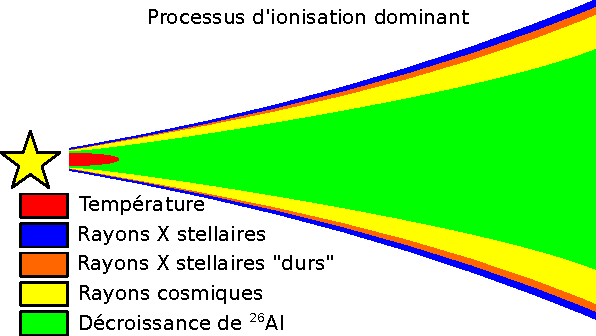
\includegraphics[width=0.49\textwidth]{figure/disk_ionization.pdf}}\hfill
\subfloat[Taux effectif d'ionisation $\zeta_\text{eff}$ par atome d'hydrogène pour un disque avec $\alpha=10^{-2}$ et $\dot{M}=10^{-7}\unit{M_\odot yr^{-1}}$. Les lignes de référence correspondent aux valeurs de $\zeta_\text{eff}$ suivante : $10^{-19}$, $10^{-21}$ et $10^{-23}\unit{s^{-1}}$. Cette figure est basée sur la figure 6 de \cite{ilgner2006ionisation1}.]{\label{fig:ilgner_ionisation}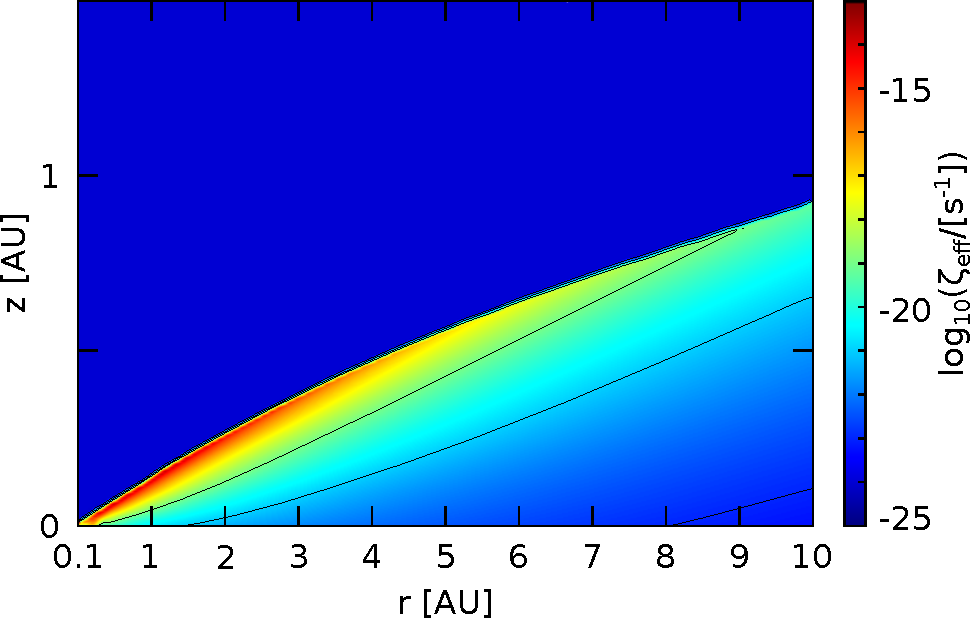
\includegraphics[width=0.49\textwidth]{figure/ilgner_ionization_rate.pdf}}
\caption[Ionisation dans un disque protoplanétaire]{Représentation de l'ionisation dans un disque protoplanétaire}
\end{figure}

On voit donc que les modèles de viscosité constante ou alpha sont incapables de rendre compte de la présence de ces zones de manière intrinsèque. Il est possible de modifier artificiellement les profils de viscosité pour faire apparaître de telles zones mais ça reste \emph{ad hoc}. Dans la suite, je n'ai pas modélisé de zone morte même s'il est probable qu'elles aient un effet sur la migration, le modèle sans zone morte n'est encore pas suffisamment bien compris pour que le rajout de ces zones sans ionisations soit pertinent.

\subsection{La poussière}\index{poussière}
Le disque protoplanétaire est principalement composé de gaz, hydrogène et hélium en majorité. Pourtant, même si la poussière ne représente qu'environ 1\% de la masse du disque elle joue un rôle au moins aussi important que le gaz lui-même.

À cause de la pression quasi-inexistante dans le disque en raison des faibles densités, solide et gaz sont les seules phases existantes, il n'y a pas de liquides dans l'espace. La poussière représente la matière solide du disque, en grains plus ou moins fin, allant du nanomètre, micromètre, jusqu'à des tailles planétaires en fin de formation. 

Cette poussière est un composé extrêmement complexe à modéliser. Elle contient différents composés solides en fonction de la température (à certaines températures et densité des composés se volatilisent et d'autres non). La ligne des glaces représente la distance à partir de laquelle de la glace d'eau apparait, augmentant de manière drastique la quantité de poussière dans le disque. 

Le disque évoluant au cours du temps, la ligne des glace évolue elle aussi à mesure que les propriétés du disque, et en particulier son profil de densité de gaz change \citep{dodsonrobinson2009icelines}.

\bigskip

De plus, la poussière est aussi responsable de l'opacité du disque, c'est-à-dire sa capacité à laisser passer ou non la lumière. À travers l'opacité, la poussière a donc une influence sur la température du disque qui se refroidit plus ou moins efficacement, et qui absorbe le rayonnement stellaire plus ou moins efficacement. 

\subsection{Opacité du disque}\label{sec:opacity}\index{opacité}
Un paramètre crucial des modèles de disques protoplanétaires est l'opacité du disque qui représente l'absorption du rayonnement incident par une cellule de gaz. Cette dernière dépend principalement de la composition chimique de la poussière sauf quand la température devient suffisamment importante pour que la totalité de la poussière se sublime, généralement au delà de $1500\unit{K}$ \citep{pollack1994composition}, l'opacité étant alors régie par les molécules du gaz.

En fonction de la température et de la pression, différentes espèces se condensent ou se subliment, modifiant les propriétés de la poussière (notamment la quantité de poussière disponible) et donc l'opacité.

L'opacité dépend de plus de la longueur d'onde, les raies d'absorptions n'étant pas uniformément réparties sur toute la gamme de longueur d'onde. Ce dernier paramètre est généralement intégré dans des modèles d'opacité. Citons notamment les opacités moyennes de Planck et de Rosseland, principales opacités utilisées dans les disques. Ce sont des quantités moyennées sur tout un spectre, rendant les opacités indépendantes de la longueur d'onde. 

Dans le cas de l'opacité de la moyenne de Rosseland, on fait l'approximation que le disque est optiquement épais, de sorte qu'on puisse négliger le flux total pour se concentrer uniquement sur la dérivée du flux. c'est-à-dire, en d'autres termes, que seul le flux provenant du gaz environnant arrive jusqu'à la zone considérée, le reste étant absorbé. Dû à l'aspect optiquement épais du disque, on perd l'information sur le flux total, ce qui simplifie les calculs. L'opacité moyenne de Rosseland $\moy{\kappa_R}$ est alors définie comme : 
\begin{align}
\inv{\moy{\kappa_R}} &= \inv{\int_0^\infty \pd{B_\nu}{T}\dif \nu} \int_0^\infty \frac{\pd{B_\nu}{T}}{\kappa_\nu}\dif \nu
\end{align}
où $B_\nu$ et $\kappa_\nu$ sont l'intensité et l'opacité spécifique (dépendant de la fréquence).

À l'inverse, les opacités de Planck concernent les disques optiquement minces, où on ne peut plus considérer uniquement la dérivée du flux. La moyenne est alors effectuée sur l'intensité spécifique directement : 
\begin{align}
\inv{\moy{\kappa_P}} &= \inv{\int_0^\infty B_\nu\dif \nu} \int_0^\infty \frac{B_\nu}{\kappa_\nu}\dif \nu
\end{align}
où $\int_0^\infty B_\nu\dif \nu$ représente l'intensité totale, tandis que $B_\nu$ et $\kappa_\nu$ sont l'intensité et l'opacité spécifique (dépendant de la fréquence).

Dans la pratique, on fait bien souvent l'approximation que le disque est optiquement épais, ce qui est généralement vrai dans les parties internes du disque ($0.1-15\unit{UA}$), lieu de formation des planètes. Pour autant, le calcul des opacités est loin d'être trivial et plusieurs modèles proposent des tables d'opacités dont le détail des propriétés est différent. Le choix du modèle a donc des implications importantes sur le modèle de formation planétaire comme je le détaillerai dans la partie \refsec{sec:influence_opacity_table}. 

En formation planétaire, le modèle le plus utilisé est \citep{bell1994FU}. Mais dans mes études, j'ai utilisé en tout et pour tout 4 modèles différents \citep{bell1994FU, zhu2009nonsteady, chambers2009analytic, hure2000transition}. À noter que \citep{bell1994FU, zhu2009nonsteady} sont des modèles qui proposent différents fonctions analytiques pour définir une opacité par morceaux. \citep{chambers2009analytic} propose un modèle très simple à opacité constante $\kappa=3$ tant que la température est inférieure à $1380\unit{K}$, puis une simple loi de puissance, fonction uniquement de la température au delà. Enfin, le modèle dans \citep{hure2000transition} ne définit pas de fonctions par morceaux mais utilise simplement une table d'opacité fonction de la température et de la densité. L'avantage de ce type de méthode est qu'on ne rajoute pas d'incertitudes par des ajustements en loi de puissance, c'est donc principalement pour ça que j'ai choisi cette table d'opacité pour mon modèle standard. 

\subsection{Profil de densité de surface}
Un point crucial dans la modélisation physique d'un disque protoplanétaire est son profil de densité de surface $\Sigma$. Ça signifie d'une part qu'on fait l'approximation d'un disque mince, et que toutes les quantités qu'on considère par la suite sont moyennées selon la direction verticale $z$.

Que l'on fasse évoluer la densité de surface ou non, on doit choisir un profil initial. Ce profil est généralement sous forme d'une loi de puissance de la forme : 
\begin{align}
\Sigma(R) &= \Sigma_0 \cdot \left(\frac{R}{R_0}\right)^{-\alpha}
\end{align}

Un profil largement utilisé est celui de la Masse Minimale de la Nébuleuse Solaire\footnote{MMSN : Minimum Mass Solar Nebulae} \citep{weidenschilling1977distribution, hayashi1981structure}. Dans cet article, le profil de densité est calculé à partir de la masse des planètes. La quantité de solide contenu dans les planètes est répartie dans des anneaux en lieu et place des planètes, puis à partir d'un rapport gaz sur poussière, le profil de densité de surface du gaz est calculé, puis approximé par une loi de puissance, ce qui donne : 
\begin{align}
\Sigma(R) &= 1700 \left(\frac{R}{1\unit{UA}}\right)^{-\sfrac{3}{2}} \unit{g/cm^2}
\end{align}
La première chose, c'est que c'est une masse minimale, c'est-à-dire qu'on suppose que toute la masse de poussière présente dans le disque de gaz se retrouve dans la masse finale des planètes, ce qui est hautement improbable, que ce soit à cause notamment de l'accrétion sur l'étoile ou de la disparition d'embryons de planètes soit en tombant dans l'étoile, soit par éjection du système.

Ce profil est malgré tout une base de travail, vu qu'il est extrêmement difficile de déduire ces informations des observations des disques. Malgré tout, les études semblent montrer que l'on s'attend à un profil moins abrupt que $\Sigma\propto r^{-\sfrac{3}{2}}$, plus proche de $\Sigma\propto r^{-1}$ \citep{bell1997structure}.

Mais on voit quand même que l'on a une grande liberté sur la densité de surface du disque, à la fois parce qu'on sait à ce jour peu de chose à ce sujet, mais aussi et surtout parce qu'au cours de son évolution, le disque de gaz va voir sa densité de surface varier énormément. En variant le profil, on étudie donc aussi différentes étapes de formation d'un même disque. 

Le profil de densité de surface, que ce soit au travers de $\Sigma_0$ ou de l'indice $\alpha$ de la loi de puissance a une grande influence sur les autres paramètres du disque, notamment le profil de température, au travers du chauffage visqueux notamment. 

Il est aussi crucial de garder à l'esprit que la loi de puissance n'est qu'un modèle, issu notamment des observations qui sondent les parties externes des disques, au delà de plusieurs dizaines d'unités astronomiques. Extrapoler ces lois de puissances jusqu'aux parties les plus internes est une très grande approximation qui a des conséquences importantes pour les planètes, dont le lieu de formation se situe vraisemblablement dans les parties internes.

\subsection{Limites et approximations dues à la modélisation}
Tout d'abord, le bord interne est une des parties les plus complexes d'un disque protoplanétaire. Ce bord interne correspond à des zones différentes pour le gaz ou pour la poussière. La poussière disparait quand la température du disque dépasse $1500\unit{K}$ environ, température au delà de laquelle la partie réfractaire des grains se sublime. 

Le gaz, quant à lui, ne se propage pas non plus jusqu'à la surface de l'étoile en raison du champ magnétique important autour des jeunes étoiles. Le bord interne est ainsi déterminé par le rayon de corotation de l'étoile, c'est-à-dire la distance à laquelle une particule en rotation képlerienne orbite à la vitesse de rotation de l'étoile. Le champ magnétique de l'étoile tournant à la vitesse de rotation de l'étoile, ce rayon de corotation correspond ainsi au rayon en dessous duquel le gaz est freiné par le champ magnétique et est rapidement accrété le long des lignes de champ. 

\bigskip

En considérant un système \og étoile + disque\fg isolé, il n'y a pas d'arrêt brutal de la distribution de matière au bord externe qui est donc plutôt une limitation numérique nécessaire aux simulations. La réalité est représentée plus fidèlement par une décroissance continue de la matière, difficile à modéliser tant pour le bord externe que pour la distribution azimutale du disque. 

Généralement, on considère donc que la taille verticale du disque est égale à une échelle de hauteur (grandeur caractéristique de la décroissance exponentielle verticale de la densité de matière), tandis que la taille radiale du disque dépend de la physique que l'on considère. Dans mon cas j'ai souvent pris un bord externe à $100\unit{UA}$.

Je vais ici essayer de récapituler les approximations qui ont été faites jusque-là sur la physique des disques, et qui vont se retrouver implicitement dans tout code qui implémente les équations décrites ci-dessus : 
\begin{enumerate}
\item On suppose que les disques évoluent de manière isolée. Les études suggèrent que les étoiles se forment majoritairement dans des amas (clusters) à l'intérieur desquels la plupart des étoiles font partie de systèmes binaires ou multiples \citep{duquennoy1991multiplicity}. Même si cette approximation permet la modélisation de l'évolution du disque, il est probable que des effets de voisinages aient des conséquences dans tout ou partie des systèmes stellaires, en particulier au travers de la photo-évaporation supplémentaire induite par les étoiles du voisinage.
\item On néglige l'auto-gravité du disque ($M_d \lesssim \frac{H}{R}M_\star$) en considérant que la période où ce n'est pas le cas est courte devant le temps de vie du disque, et que ce dernier tend rapidement vers une configuration où l'auto-gravité est négligeable.
\item On considère que le gaz est en rotation képlerienne $\Omega=\sqrt{\frac{GM_\star}{r^3}}$. Pour cela, on néglige la pression du gaz qui a tendance à rendre la rotation légèrement sous-képlerienne.
\item On considère qu'il n'y a pas de variation de la gravité dû à la variation de masse de l'étoile induite par l'accrétion. Ça entraîne alors $\pd{\Omega}{t} = 0$.
\item Dans le calcul du chauffage visqueux, on néglige la vitesse azimutale, la vitesse radiale ainsi que toutes les dérivées en $\varphi$ compte tenu que le disque est axisymétrique.
\item On se place dans le cadre d'un disque optiquement épais quand on choisi d'utiliser des moyennes de Rosseland pour l'opacité. Si c'est physiquement cohérent avec les parties internes du disque, ça ne l'est parfois plus dans les parties externes, surtout si le disque est très étendu.
\item Le modèle d'opacité a une grande influence sur la physique du disque. En particulier, chaque modèle fait des hypothèses sur la métallicité, les propriétés de la poussière, notamment la taille des grains. Chacune de ces hypothèses joue sur l'opacité d'une manière qui est totalement masquée dans les équations ou tables qu'on utilise pour rendre compte de la dépendance de l'opacité en fonction de la température et de la densité.
\item On fait souvent l'approximation que la masse moléculaire moyenne $\mu$ est constante (et typiquement égale à $\mu=2.35$). Or en fonction des transitions d'opacité, la quantité de poussière va brusquement varier, engendrant une variation de $\mu$. Cette masse moléculaire moyenne a en particulier une importance dans le calcul de l'échelle de hauteur $H$ du disque et la vitesse du son $c_s$. 
\item Définir le profil de densité de surface du disque comme une loi de puissance reste une approximation. Ça l'est d'autant plus que le disque est étendu. Du reste, la masse du disque et l'indice de la loi de puissance sont peu contraints, donnant une grande liberté dans le profil de densité dont il faut tenir compte pour mettre en perspective les résultats que l'on obtient.
\item Le modèle choisi pour la viscosité, constante ou prescription alpha, néglige bien souvent la présence de zone morte où l'ionisation n'est pas suffisante pour que l'on puisse définir une viscosité turbulente. L'absence de ces zones dans un disque modélisé est bien entendue une approximation à des fins de simplifications, mais masque certaines propriétés intrinsèques des disques dont les conséquences sur la formation planétaire sont encore mal connues.
\item Une dernière approximation, et qui a des conséquences importantes pour l'opacité, le profil de température, la viscosité et par extension, toute la physique du disque, est le fait de considérer les propriétés de la poussière comme figées dans le temps. Au cours de la vie du disque, la poussière évolue. Sa distribution de taille change, la quantité totale de poussière est modifiée, notamment par l'accrétion. Et enfin, à mesure que la poussière se retrouve dans des embryons de planète de plus en plus gros, la quantité de poussière disponible sous la forme de petites particules diminue d'autant. 
\end{enumerate}

\section{Interaction disque-planète}
On ne peut étudier séparément le disque ou les planètes, c'est un système global, en interaction, qui évolue depuis la formation du disque (et les poussières qu'il contient) jusqu'à la dissipation du disque (et la possible présence d'une ou plusieurs planètes).

Je vais maintenant présenter les interactions principales entre les planètes et le disque qui les contient. 

\subsection{Migration des planètes de faible masse : Type I}
\index{migration!Type I}
Ce type de migration ne concerne que les planètes de faible masse (de l'ordre de $10M_{\oplus}$) pour lesquelles l'interaction de marée entre la planète et le disque a une réponse linéaire, c'est-à-dire que le profil de densité surfacique n'est quasiment pas modifié par la planète. Ces planètes, qui ne creusent pas de sillon (gap) dans le disque de gaz, vont migrer vers l'intérieur. On appelle cette migration la \gras[migration!Type I]{migration de Type I}.

%\begin{remarque}
%Pour plus de détails, se référer au chapitre 9, page 188--191 de \cite{barnes2010formation} ou \cite{ward1997protoplanet} pour l'article original.
%\end{remarque}

\subsubsection{Couple du disque sur la planète}
Un couple gravitationnel représente l'échange d'énergie associé à une force gravitationnelle.  Le couplage gravitationnel entre les ondes de densité et la planète qui les crée abouti à un couple qui agit sur la planète : 
\begin{align}
\Gamma &= - \iint_\text{disc} \left(\vect{r}\wedge\grad{\Phi_p}\right)\Sigma r \dif r \dif \theta
\end{align}

À chaque fois qu'il sera mentionné \og couple\fg, celui-ci fera référence au couple \emph{du} disque \emph{sur} la planète.

Ainsi, si le couple est négatif (sous-entendu du disque sur la planète), le disque va prendre de l'énergie à la planète qui va ainsi migrer plus proche de son étoile, vu que son énergie cinétique diminue.\index{migration}

Si le couple est positif, la planète migre vers l'extérieur, cette dernière prenant de l'énergie au disque.

\subsubsection{Couple de Lindblad}\index{couple!de Lindblad}
La présence d'une planète dans un disque de gaz entraine la création d'ondes de densités aux \gras[résonance!de Lindblad]{résonances de Lindblad} \citep{goldreich1979excitation}. Le couplage gravitationnel entre les ondes de densité et la planète qui les crée abouti à un \gras{couple} qui agit sur la planète.

\bigskip

Il est tout d'abord intéressant de remarquer l'origine des bras spiraux dans les galaxies. Ce sont essentiellement des phénomènes statistiques que l'on peut résumer en deux points : 
\begin{enumerate}
\item Une onde de densité se forme par la présence de sur-densité locales comme des nuages de gaz géants \citep{donghia2013self}. Une fois formée, il est possible que l'onde de densité s'auto-entretienne en modifiant les excentricités des éléments qui la composent \citep{binney2008book}.

\item L'onde ainsi créée n'est pas une onde matérielle rigide en rotation, mais une onde de densité statistique. Le bras spiral n'est ainsi pas constitué d'une population fixe d'étoile. Les étoiles constituant le bras spiral changent avec le temps, mais statistiquement, la position des étoiles dans la galaxie dessine une onde de densité où le nombre d'étoiles est plus grand. 
\end{enumerate}

\reffig{fig:spiral_arms} schématise l'apparition d'onde de densité. Dans le cas à gauche, des orbites concentriques parfaitement circulaires sont ajoutés. On ne voit rien de particulier. Par contre, dans le cas à droite, on choisi des orbites très légèrement excentriques. À chaque étape, on rajoute une orbite en agrandissant l'orbite précédente et en la tournant légèrement. On voit ainsi apparaître deux ondes de densités dans le disque simplement dues à l'orientation des orbites excentriques.

Ça signifie en particulier que la vitesse de rotation de l'onde de densité n'est pas liée à la vitesse de rotation des étoiles qui la composent. Ceci permet de résoudre le \og winding problem\fg c'est-à-dire le fait que si l'onde de densité était rigide, elle s'enroulerait sur elle-même au bout de quelques orbites seulement, ce qui n'est pas le cas ici \citep{binney2008book}.

\begin{figure}[htbp]
\centering
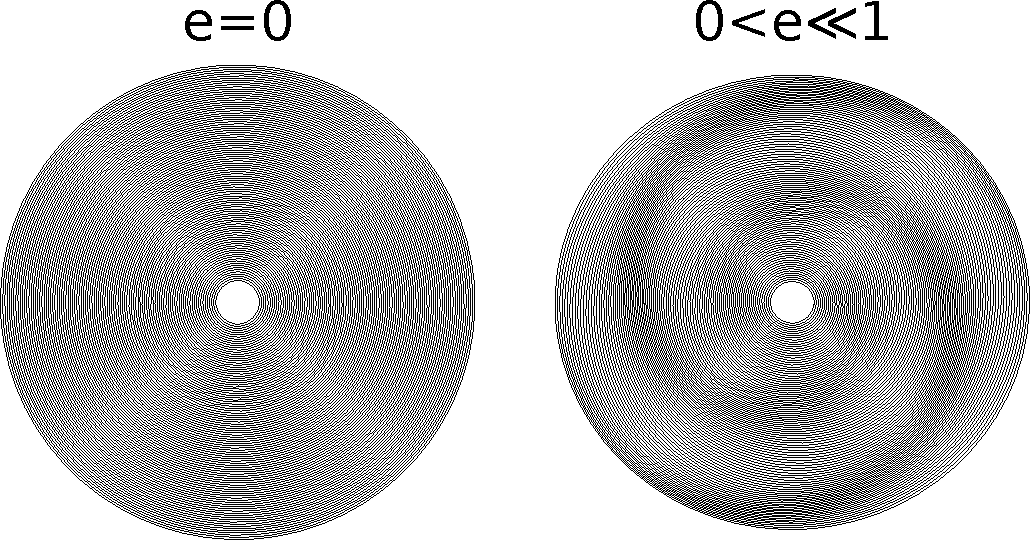
\includegraphics[width=0.9\linewidth]{figure/spiral_arms.pdf}
\caption[Origine des bras spiraux dans une galaxie.]{Illustration de l'origine des bras spiraux dans une galaxie au travers de
l'excitation cohérente de l'excentricité par les bras eux-mêmes. Dans le cas \og $e=0$\fg, les orbites des étoiles, représentées
par les traits noirs sont des cercles parfaits. Dans le cas \og $0<e\ll 1$\fg, les orbites sont toutes très légèrement
excentriques, et les arguments du périhélie légèrement décalés à mesure que les demi-grands axes
augmentent.}\label{fig:spiral_arms}
\end{figure}

\bigskip

Pour l'interaction entre une planète et un disque protoplanétaire, c'est exactement le même principe. Le potentiel de la planète excite les excentricités des éléments fluides voisins jusqu'à former une onde de densité autour de la planète. La différence principale est que le perturbateur est un potentiel gravitationnel tournant, ce qui modifie la forme des ondes de densité comme illustré \reffig{fig:lindblad_torque}. 

\begin{figure}[htbp]
\centering
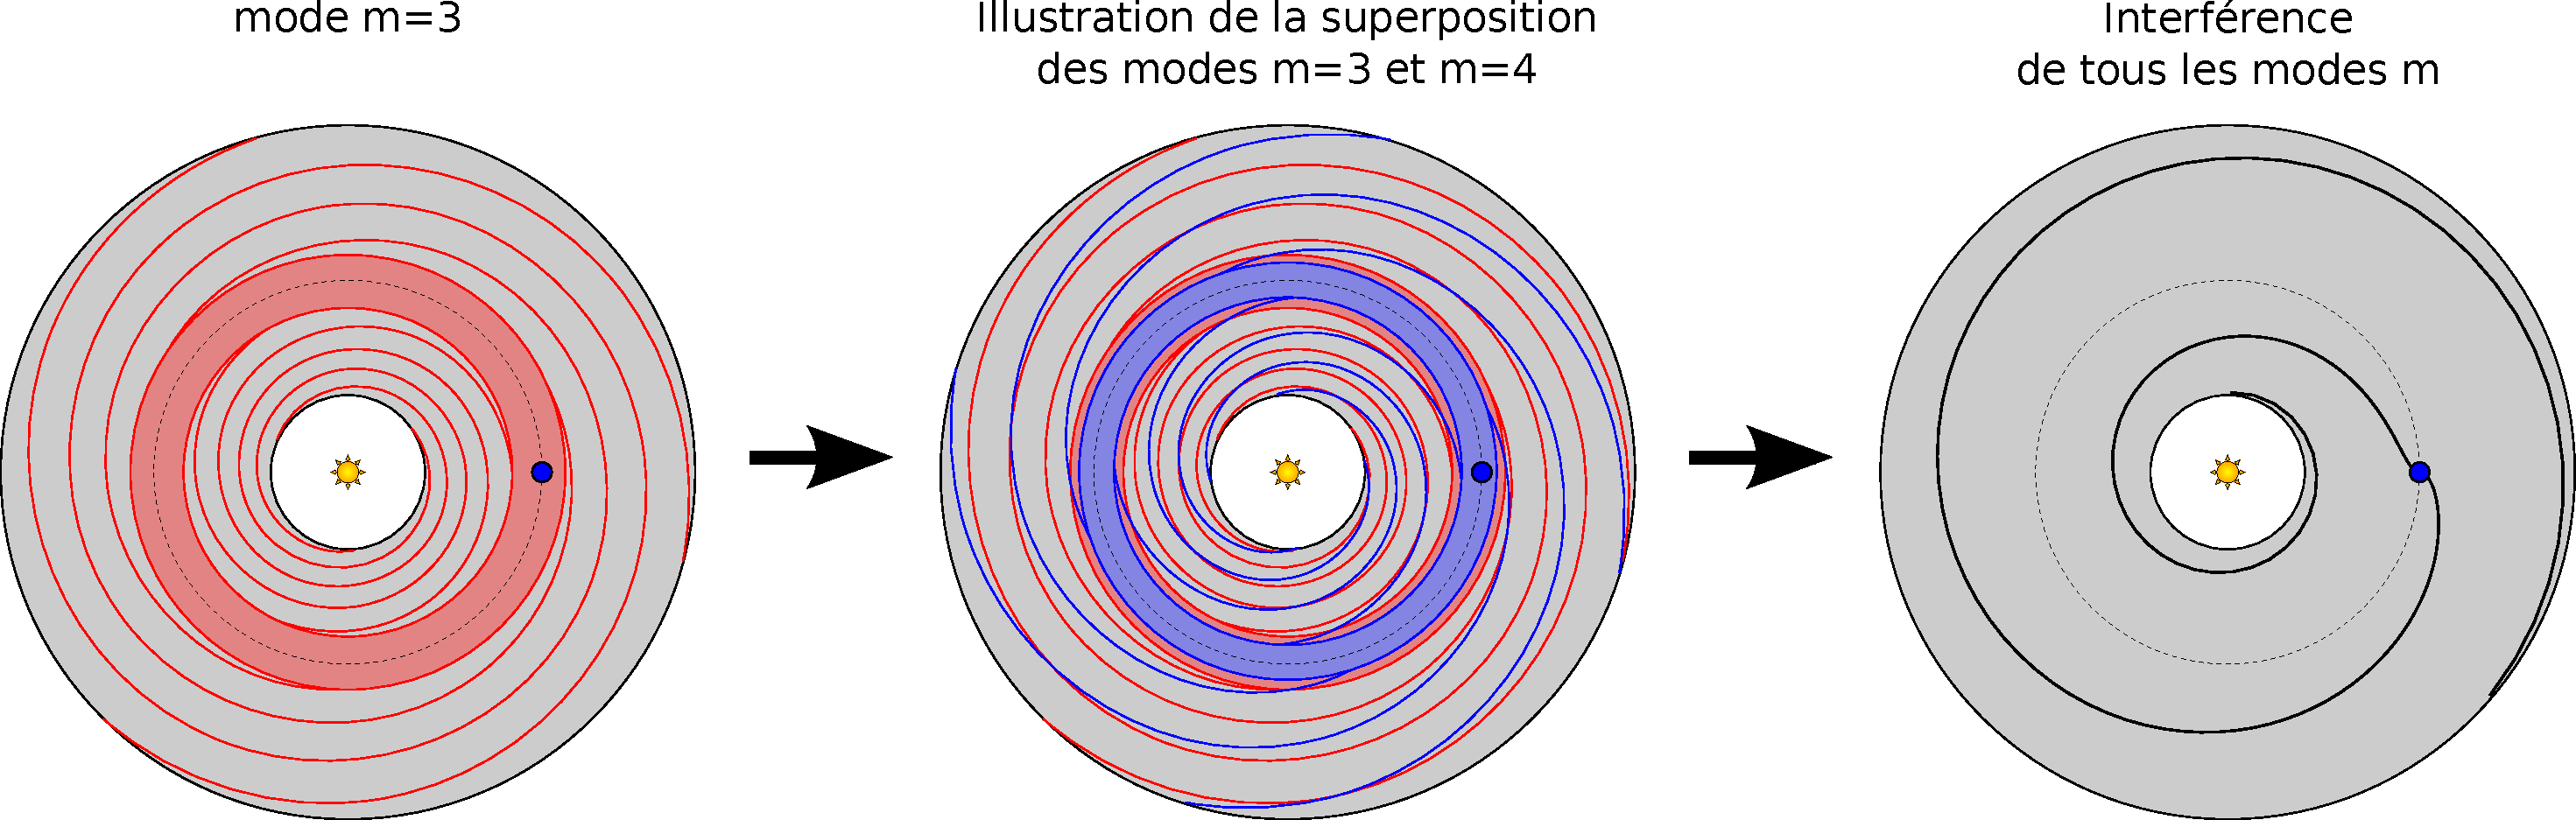
\includegraphics[width=\linewidth]{figure/lindblad_torque.pdf}
\caption[Construction de l'onde de densité due à la présence d'une planète.]{Génération d'ondes de densité dans le disque
protoplanétaire dû à la présence d'une planète. Chaque mode $m$ émet $m$ ondes de densité de part et d'autre de la position
radiale de la planète. Un anneau interne aux positions du mode $m$ est dénué de toute onde dû à ce même mode. Les interférences
entre toutes les ondes de densités de tous les modes donne deux ondes de densités que l'on observe dans des simulations
hydrodynamique. Les positions successives des interférences constructives sont données par \cite[eq. (13) et
(24)]{ogilvie2002wake}}\label{fig:lindblad_torque}
\end{figure}


% discussion avec laurent : L'explication de l'onde de densité avec les excentricités est correct. Ça permet de résoudre le problème du "winding problem", c'est-à-dire que si le bras spiral était rigide, il serait censé s'enrouler sur lui-même au fil de la rotation (vu que la rotation du bras est égale à la rotation des étoiles qui le composent), et donc au bout de quelques rotations, le bras devrait e^tre hyper enroulé. par contre, si on considère une onde de densité, qui n'existe que statistiquement, ça veut dire que les étoiles entre et sortent du bras, qui lui tourne à une vitesse qui lui est propre, et qui n'a rien à voir avec la vitesse des étoiles en elle même. La majorité des galaxies spirales sont barrées, et on pense que c'est la barre quie st à l'origine des spirales, qui démarrent au bout de la barre.

%Par un phénomène résonnant entre une cellule de gaz et un mode $m$ du potentiel gravitationnel de la planète dont on a décomposé l'expression en série de fourrier (on fait ainsi apparaître des termes de fréquence différen

Le potentiel gravitationnel de la planète peut se décomposer en série de Fourier où chaque mode $m$ (entier) a une dépendance sinusoïdale en azimut et possède $m$ maxima et $m$ minima. 

Pour chaque mode $m$ du potentiel gravitationnel de la planète, on définit deux résonances, une résonance interne (ILR : Inner Lindblad Resonance) et une résonance externe (OLR : Outer Lindblad Resonance) associées aux positions suivantes dans le cas d'un disque froid ($H/R\ll 1$ ; \cite{ward1997protoplanet}) : 
\begin{subequations}
\begin{align}
r_{OLR}(m) &= \left(\frac{m+1}{m}\right)^\sfrac{2}{3}r_p\\
r_{ILR}(m) &= \left(\frac{m-1}{m}\right)^\sfrac{2}{3}r_p
\end{align}
\end{subequations}

Pour un mode $m$ donnée, à partir des anneaux de rayon $r_{ILR}(m)$ et $r_{OLR}(m)$ vont être lancées $m$ ondes de densités. 

Dans le cas des bras spiraux dans une galaxie, c'est principalement un mode $m=2$ qui propage une onde spirale de part et d'autre d'une barre centrale source des ondes de densité. Dans le cas d'une planète dans un disque, des ondes de densité sont lancées pour chaque mode $m$. 

Par interférence constructive \citep{ogilvie2002wake}, la somme de toutes les ondes de densités émises par tous les modes du potentiel gravitationnel résulte en la formation d'une onde de densité résultante \reffig{fig:lindblad_torque}. 

\bigskip

Il est important de remarquer que la position de la résonance externe d'ordre $m$ est systématiquement plus proche que la résonance interne associée. Ainsi, en sommant sur tous les modes, on arrive à la conclusion que le couple total externe l'emporte toujours sur le couple total interne \citep{ward1997protoplanet}. 

Ainsi, le couple de Lindblad est généralement négatif pour des modèles typiques de disques protoplanétaires \citep{ward1997protoplanet}.

La résolution numérique des équations linéarisées permet de trouver une formule analytique pour le couple de Lindblad $\Gamma_L$. Dû à la résolution numérique qui doit s'affranchir de la divergence du potentiel gravitationnel en $r=r_0$, cette formule introduit une longueur de lissage permettant de contourner la singularité du noyau du Green du potentiel gravitationnel \citep[eq. (14)]{paardekooper2010torque} : 
\begin{align}
\gamma \Gamma_L/\Gamma_0 &= - \left(2.5 +1.7\beta -0.1d\right) \left(\frac{0.4}{b/h}\right)^{0.71}\label{eq:lindblad-torque}
\end{align}
où $\gamma$ est l'indice adiabatique, $b/h$ le paramètre de lissage du potentiel gravitationnel, et $\beta$ et $d$ sont les exposants des lois de puissance pour les profils de température et de densité de surface. 

Le couple est ici exprimé en unité de $\Gamma_0$, couple de référence défini par : 
\begin{align}
\Gamma_0 &= \left(\frac{q}{h}\right)^2\Sigma_p {r_p}^4 {\Omega_p}^2
\end{align}

Notons aussi que le processus physique du transport du moment cinétique de la planète est réalisé par l'onde de densité. Le moment cinétique est emporté par l'onde de densité qui l'échange avec le gaz environnant à mesure que ce dernier amorti et dissipe l'onde.

\subsubsection{Couple co-orbital ou de corotation}\index{couple!de corotation}\label{sec:couple-corotation}
\begin{figure}[htbp]
\centering
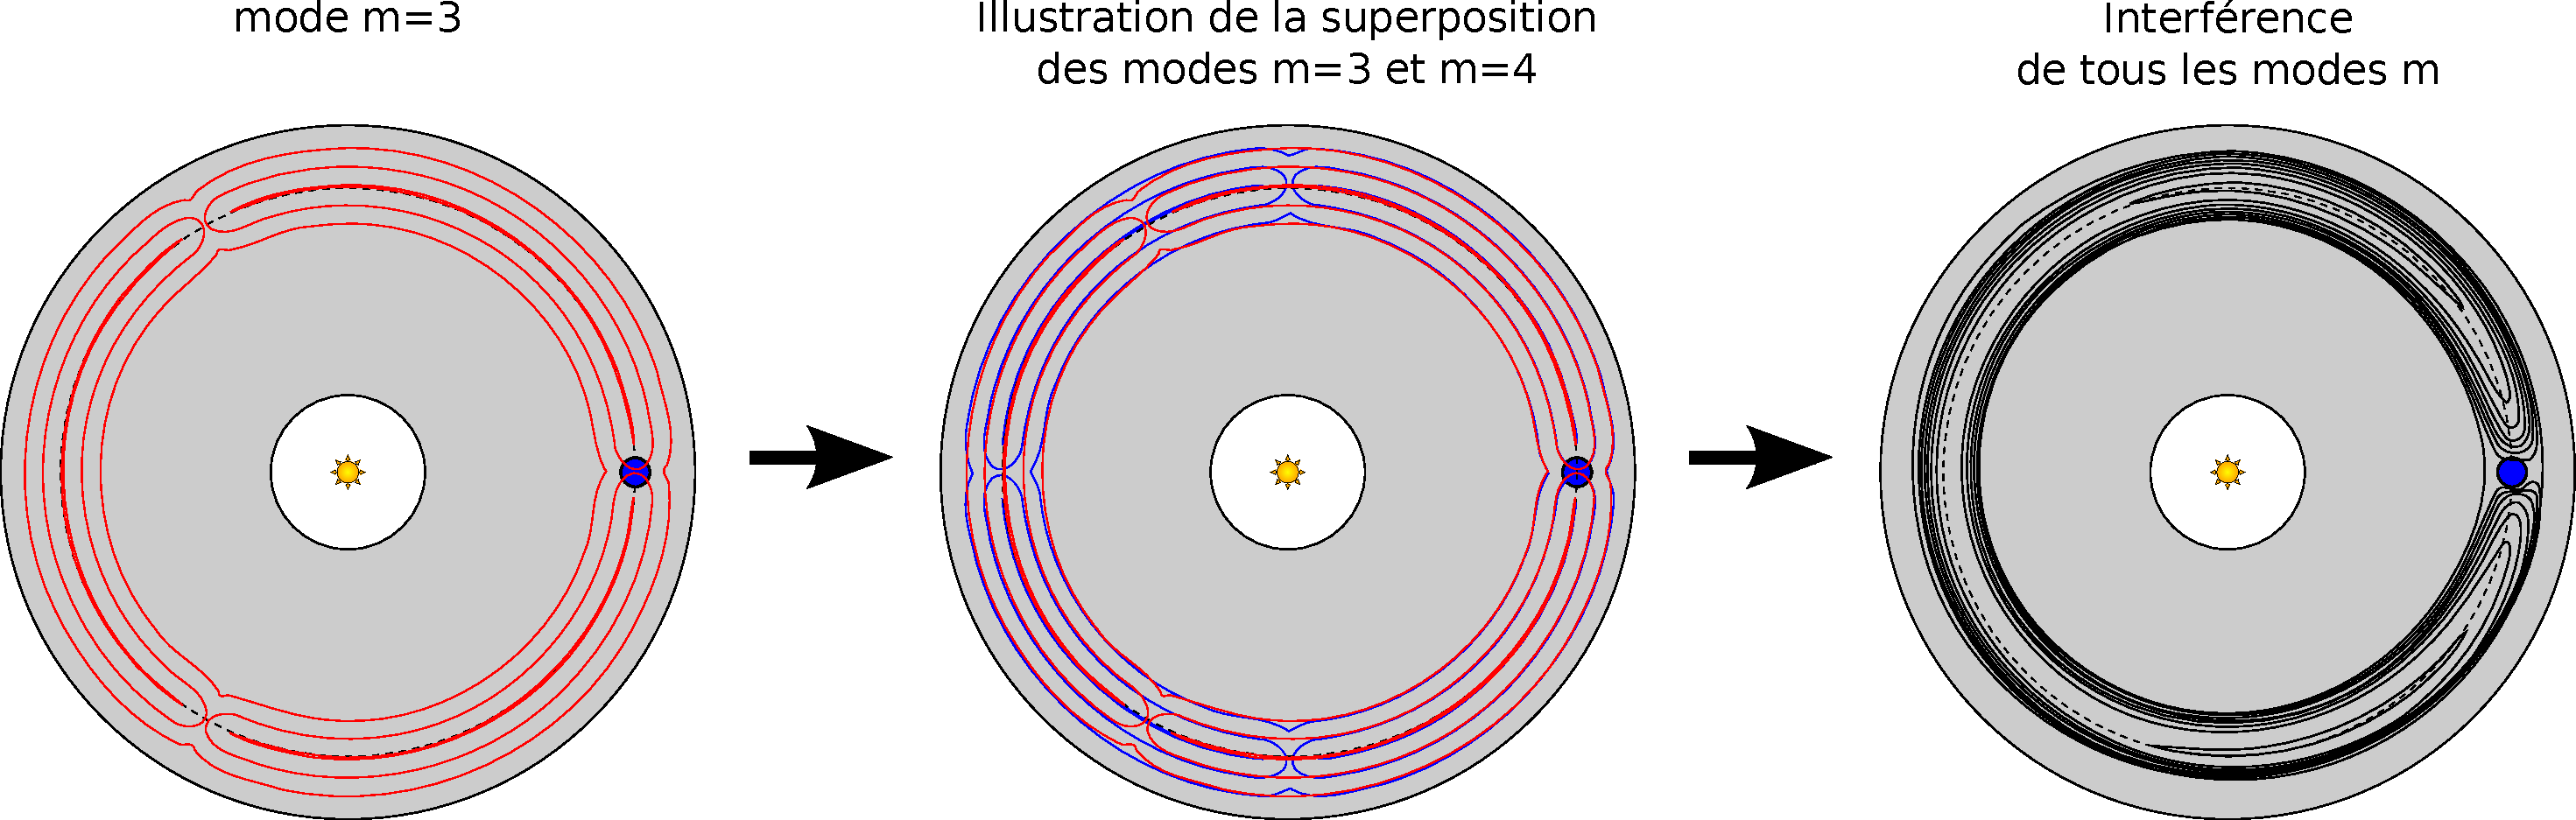
\includegraphics[width=\linewidth]{figure/corotation_modes.pdf}
\caption[Zone de corotation d'une planète.]{À partir de la décomposition en série de Fourier du potentiel
gravitationnel de la planète, chaque mode $m$ a pour conséquence $m$ zones de libration dans la zone de corotation avec la
planète. Les interférences entre l'infinité de modes $m$ fait apparaître des orbites fer-à-cheval (\og horseshoe orbits\fg) dans
le référentiel tournant avec la planète. La zone de corotation a ici été exagérée pour plus de
lisibilité.}\label{fig:corotation_torque}
\end{figure}

De la même manière que précédemment pour le couple de Lindblad, on peut repartir de la décomposition en série de Fourier du potentiel gravitationnel de la planète. Pour chaque mode $m$ de la décomposition, on voit apparaître $m$ zones de libration, centrées sur le rayon de la planète, et réparties en azimut. \reffig*{fig:corotation_torque} représente le mode $m=3$, puis une juxtaposition de mode et finalement le résultat des interférences constructives entre tous les modes $m$ de la décomposition.


Le couple de corotation provient des échanges gravitationnels que va avoir une particule fluide en co-orbite avec une planète. Il existe deux types de couples, issus du gradient de deux quantités physiques distinctes, la vorticité spécifique (vorticité divisée par la densité de surface) appelée parfois vortensité et l'entropie. 

Chacun de ces deux couples possède une partie qui peut saturer en fonction des conditions physiques. 

Pour illustrer le principe de la saturation, et sans considérer un couple en particulier, il convient de définir certains temps caractéristiques afin de comprendre l'origine de ce couple non saturé, et pourquoi ce dernier peut saturer. \reffig*{fig:corotation_orbits} représente schématiquement les 3 temps principaux mis en jeux. 

\begin{figure}[htbp]
\centering
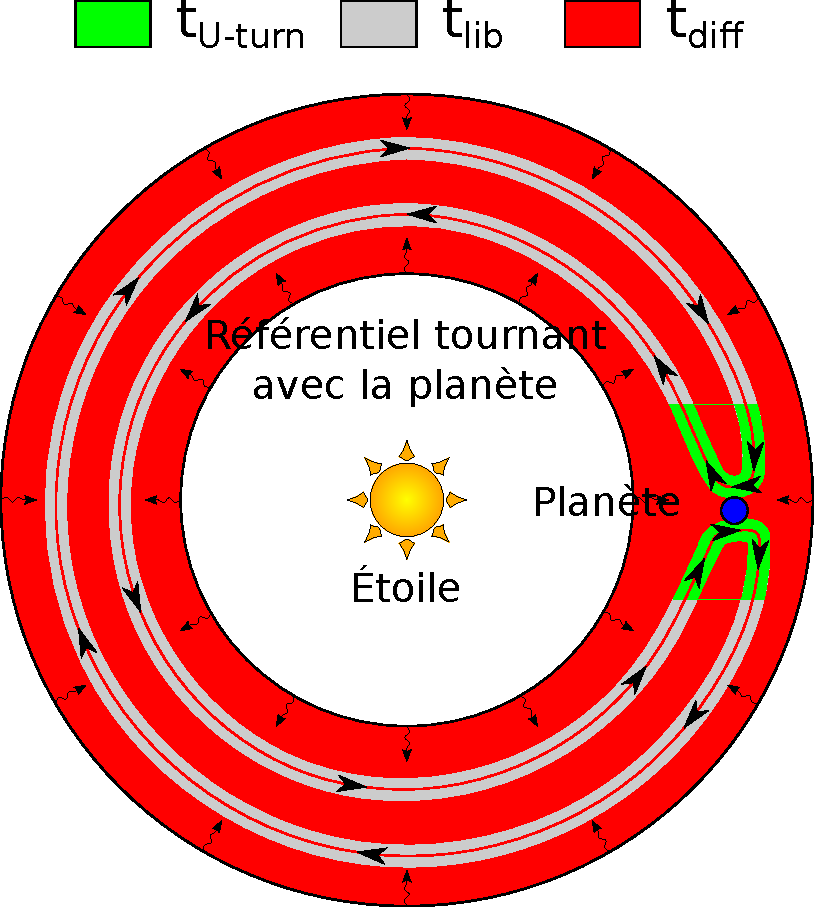
\includegraphics[width=0.75\linewidth]{figure/corotation_times.pdf}
\caption[Temps caractéristiques mis en jeu dans la zone de corotation.]{Dans le référentiel tournant avec la planète (qui est
donc fixe dans ce repère), représentation d'une orbite de corotation ainsi que des différents temps caractéristiques mis en
jeux. $t_\text{lib}$ est le temps mis par un élément fluide pour effectuer une orbite de corotation. $t_\text{U-turn}$ est le
temps mis par un élément fluide pour effectuer un demi-tour devant la planète. $t_\text{diff}$ peut être suivant le cas le temps
radiatif $t_\text{rad}$ ou le temps visqueux $t_\text{vis}$ nécessaire pour homogénéiser les propriétés thermodynamiques de
l'élément fluide avec son environnement.}\label{fig:corotation_orbits}
\end{figure}

On définit tout d'abord $t_\text{lib}$ comme le temps mis par un élément fluide pour effectuer une co-orbite complète dans la zone de fer-à-cheval. Ceci dépend de la distance de l'élément fluide au rayon de corotation. Mais le temps de libration le plus court est obtenu à la distance $x_s$ de la corotation, et vaut \citep[eq. (52)]{baruteau2008corotation} : 
\begin{align}
t_\text{lib} &= \frac{4\pi}{x_s\abs{\od{\Omega}{r}}} = \frac{8\pi r_p}{3\Omega_p x_s}
\end{align}
où $x_s$ est la demi-largeur de la zone de fer-à-cheval (\og half-width of the horseshoe region\fg) \citep[eq. (44)]{paardekooper2010torque} :
\begin{align}
\frac{x_s}{r_p} &= \frac{1.1}{\gamma^{1/4}} \left(\frac{0.4}{b/h}\right)^{1/4} \sqrt{\frac{q}{h}}
\end{align}
Dans le cas d'une planète de $20\unit{M_\oplus}$ à $1\unit{UA}$ dans un disque avec $h=0.05$ et $M_\star=1M_\odot$, ce temps de libration vaut $t_\text{lib}\sim 38 p_\text{orbital}$. 

Le temps $t_\text{U-turn}$ représente quant à lui la durée nécessaire à un élément fluide pour effectuer un demi-tour devant la planète, c'est-à-dire pour parcourir la zone de longueur $2x_s$\footnote{$x_s$ est la demi-largeur de la zone de fer-à-cheval (\og half-width of the horseshoe region\fg)} devant la planète. Il est définit par \citep[eq. (64)]{baruteau2008corotation}
\begin{align}
t_\text{U-turn} &\simeq \frac{4}{\Omega_p}\left[\frac{H(r_p)}{R_H}\right]^\sfrac{3}{2}
\end{align}
où $R_H=r_p (q/3)^{1/3}$ est le rayon de Hill de la planète. Dans le cas d'une planète de $20\unit{M_\oplus}$ à $1\unit{UA}$ dans un disque avec $h=0.05$ et $M_\star=1M_\odot$, ce temps vaut $t_\text{U-turn} \sim 1.6 p_\text{orbital}$.

Un troisième est dernier temps $t_\text{diff}$ rentre en jeu, c'est le temps de diffusion. Selon le processus physique mis en jeu, ce temps peut être $t_\text{rad}$ ou $t_\text{visc}$.

$t_\text{rad}$ représente le temps de diffusion par refroidissement radiatif. Ce temps est plus long quand on se rapproche de l'étoile car le rayonnement est plus rapidement réabsorbé. Le temps radiatif au travers de la zone de corotation est de l'ordre de :
\begin{align}
t_\text{rad} &= \frac{{x_s}^2}{\chi}
\end{align}
où $x_s$ est la demi-largeur de la zone de corotation et $\chi$ est la diffusivité thermique.
 
$t_\text{visc}$ représente la diffusion d'une quantité physique par la viscosité. Ce temps est plus court quand on se rapproche de l'étoile. Le temps visqueux à la zone de corotation $t_\text{visc}$ est  de l'ordre de \citep{masset2001coorbital, masset2002coorbital, ogilvie2003saturation}
\begin{align}
\tau_\nu &\sim \frac{{x_s}^2}{\nu}
\end{align}

Quand la grandeur physique considérée est la vortensité (ou vorticité spécifique), seul $t_\text{visc}$ est à prendre en compte. Quand c'est l'entropie, les deux temps $t_\text{visc}$ et $t_\text{rad}$ sont importants. \reffig*{fig:corotation_orbits} récapitule les temps mis en jeux et à quoi ils correspondent.

\bigskip

Pour que le couple de corotation soit non saturé, on doit satisfaire aux inéquations suivantes \citep[eq. (31)]{baruteau2013recent} :
\begin{align}
t_\text{U-turn} < t_\text{diff} < \frac{t_\text{lib}}{2}
\end{align}
$t_\text{U-turn}$ est le temps nécessaire pour faire le demi-tour devant la planète (pour traverser une zone égale approximativement à $2x_s$). $t_\text{lib}$ est le temps de libration, c'est-à-dire le temps mis par une particule fluide pour faire le tour de la zone en fer-à-cheval. $t_\text{diff}$ quant à lui est le temps de diffusion de la quantité physique considérée. Suivant les cas, il peut y avoir plusieurs temps de diffusion qui sont importants, auquel cas les inégalités doivent être satisfaites pour tous les temps de diffusions mis en jeux.

\begin{figure}[htbp]
\centering
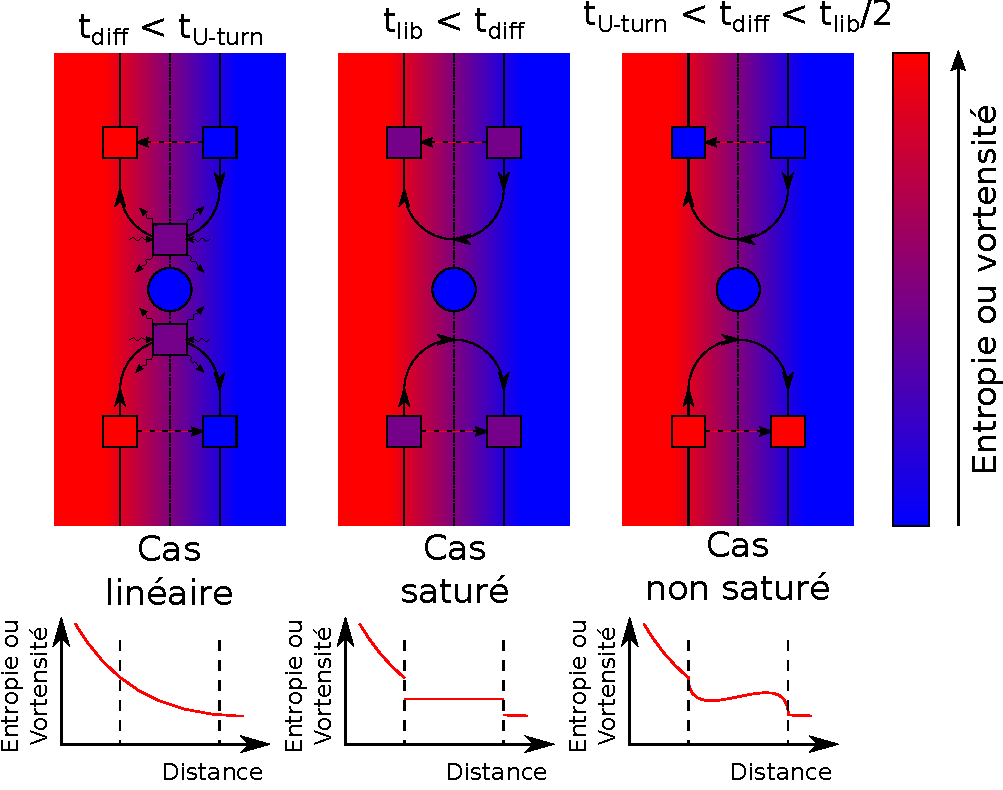
\includegraphics[width=0.75\linewidth]{figure/corotation_principle.pdf}
\caption[État du couple de corotation en fonction des valeurs des temps caractéristiques.]{Dans le référentiel tournant avec la
planète, représentation du mécanisme général à l'origine du couple de corotation. Lorsque les temps de diffusion $t_\text{diff}$
sont plus grands que le temps de libration $t_\text{lib}$, le couple de corotation sature car le gradient de vortensité/entropie
au travers de la région fer-à-cheval tend à s'aplatir. Ce dernier est restauré quand les temps de diffusion $t_\text{diff}$ sont
plus courts que le temps de libration $t_\text{lib}$. Dans ce cas, la valeur optimale du couple de corotation est obtenue
lorsque les temps de diffusion $t_\text{diff}$ sont de l'ordre de la moitié du temps de libration $t_\text{lib}/2$. Dans la
limite où les temps de diffusion $t_\text{diff}$ sont plus courts que le temps de demi-tour $t_\text{U-turn}$, l'amplitude du
couple de corotation décroit pour atteindre la valeur prédite par une analyse linéaire.}\label{fig:corotation_principle}
\end{figure}

\reffig*{fig:corotation_principle} illustre les trois cas possibles en fonction des commensurabilités entre les différents temps caractéristiques mis en jeux.

L'idée générale afin d'éviter la saturation, c'est qu'on doit restaurer le gradient d'entropie / de vortensité au travers de la zone fer-à-cheval. Il faut donc que les processus diffusifs soient suffisamment efficace pour qu'en arrivant à la région de \og U-turn\fg de l'autre côté, l'élément fluide ait pu équilibrer ses conditions physiques avec le milieu environnant. Cette condition est illustrée par l'inégalité suivante : 
\begin{align}
t_\text{diff} < \frac{t_\text{lib}}{2}
\end{align}

Mais il faut de plus que la diffusion ne soit pas trop efficace, sous peine que la valeur du couple de corotation diminue pour atteindre la valeur prédite par une analyse linéaire. Ceci donne alors la deuxième inéquation : 
\begin{align}
t_\text{U-turn} < t_\text{diff}
\end{align}

\bigskip

De la même manière que pour le couple de Lindblad, la résolution numérique des équations nous permet d'avoir des expressions analytiques pour les couples de corotation. 

Il y a d'une part les couples soumis à saturation \citep[eq. (45)]{paardekooper2010torque} :
\begin{subequations}
\begin{align}
\gamma \Gamma_\text{c,hs,baro}/\Gamma_0 &= 1.1\left( \frac{3}{2} - d\right)\left(\frac{0.4}{b/h}\right)\\
\gamma \Gamma_\text{c,hs,ent}/\Gamma_0 &= \frac{\xi}{\gamma}\left(10.1\sqrt{\frac{0.4}{b/h}} - 2.2\right)\left(\frac{0.4}{b/h}\right)
\end{align}\label{eq:saturated-corotation-torque}
\end{subequations}
et les couples non soumis à saturation, dits linéaires \citep[eq. (17)]{paardekooper2010torque} :
\begin{subequations}
\begin{align}
\gamma \Gamma_\text{c,lin,baro}/\Gamma_0 &= 0.7\left( \frac{3}{2} - d\right)\left(\frac{0.4}{b/h}\right)^{1.26}\\
\gamma \Gamma_\text{c,lin,ent}/\Gamma_0 &= \xi\left[2.2\left(\frac{0.4}{b/h}\right)^{0.71} - \frac{1.4}{\gamma}\left(\frac{0.4}{b/h}\right)^{1.26}\right]
\end{align}\label{eq:linear-corotation-torque}
\end{subequations}
$d$ et $\xi=\beta - (\gamma-1)d$ sont respectivement les négatifs des exposants des lois de puissance pour les profils 1D de densité de surface et d'entropie.

\bigskip

Dans la pratique, ce couple peut être positif (migration vers l'extérieur) ou négatif (migration vers l'intérieur) en fonction des variations des quantités physiques par rapport à leur valeur nominales.

\subsubsection{Modélisation dans le code N-corps}
Les couples de Lindblad et de Corotation ont été intégrés aux simulations numériques en utilisant le modèle de \cite{paardekooper2011torque}. Plus de détails sur l'implémentation de ces formules et le modèle de disque utilisé dans la section \refsec{sec:code_n-corps}.

\subsection{Migration des planètes massives : Type II}\index{migration!Type II}
Par massive, on entend une planète qui va induire des modifications importantes du profil de densité du disque. L'approximation du régime linéaire n'est alors plus valable. 

Je présente ici très succinctement ce type de migration que je n'ai pas considéré tout au long de ma thèse. Je me place dans le régime linéaire et me suis concentré sur les cœurs de planète géante et les planètes telluriques. J'ai donc négligé tous les effets non-linéaires dû aux grandes masses, et en particulier la création d'un sillon par les planètes.

\bigskip

Quand une planète dans un disque devient suffisamment massive, la réponse du disque n'est plus linéaire, et des ondes de densité induites par la planète forment des chocs non loin de là où elles sont émises. La répulsion entre le disque et la planète devient si forte qu'une cavité annulaire se forme autour de l'orbite de la planète, creusant le disque de gaz \citep{lin1986tidal}.

Une fois que la cavité est formée, la planète est dite en migration de \gras[migration!Type II]{Type II} : son orbite agit alors essentiellement comme une barrière entre les deux parties du disque de gaz, \emph{interne} et \emph{externe}. Du gaz peut sauter le gap \citep{lubow2006gas}, ou être accrété par la planète mais cette dernière voit son mouvement régit par le disque de gaz, se retrouvant entraînée par la migration de celui-ci.

Quand la planète creuse un sillon et que sa masse est inférieure ou de l'ordre de la masse locale du disque ($M_p \lesssim M_\text{d,loc}$ avec lequel elle interagit, alors le temps de migration de la planète est contrôlé par le temps visqueux du disque, car cette dernière se comporte comme une particule de ce disque \citep{nelson2000migration}.

\bigskip

Pendant que le gap dû à la planète est en train de se creuser, il peut y avoir un fort couple de corotation négatif \citep{masset2003runaway}. Ce mode de migration intermédiaire est parfois appelé migration de \gras[migration!Type III]{Type III}. 

\subsection{L'amortissement de l'excentricité et de l'inclinaison}\index{amortissement!excentricité}\index{amortissement!inclinaison}%circularisation
%Penser aux papiers cresswell et al. 2007 et tanaka et al. 2004
Une planète sur une orbite non-circulaire $e\neq 0$ génère des ondes supplémentaires à cause de son excentricité. De même, une orbite légèrement inclinée induit des ondes à cause de l'inclinaison $I$ de la planète. 

Des calculs analytiques sur les équations linéarisées (valables quand $e$ et $I$ sont faibles $e,i \ll H/R$) montrent que les ondes dues à l'excentricité ou l'inclinaison ont tendance à amortir l'élément orbital qui est à leur origine. \cite[eqs. (45), (47)]{tanaka2004three} trouvent un amortissement exponentiel dont les temps caractéristiques sont : 
\begin{subequations}
\begin{align}
\frac{\overline{\dot{e}}}{e} &= -\frac{0.780}{t_\text{wave}}\\
\frac{\overline{\dot{I}}}{I} &= -\frac{0.544}{t_\text{wave}}
\end{align}
\end{subequations}
où le temps caractéristique de l'évolution orbitale $t_\text{wave}$ est donné par \cite[eq. (49)]{tanaka2004three} :
\begin{align}
t_\text{wave} &= \frac{M_\star}{M_p}\frac{M_\star}{\Sigma_p a^2} \left(\frac{H}{R}\right)^4 {\Omega_p}^{-1}
\end{align}

Le temps caractéristique d'amortissement pour l'excentricité et l'inclinaison est similaire et de l'ordre de \citep{tanaka2004three} :
\begin{align}
\tau_e \sim \tau_I &\sim h^2 \tau_\text{mig}
\end{align}

Des simulations hydrodynamiques montrent que le même phénomène d'amortissement se produit pour des valeurs plus grandes de $e$ et $I$, tout en étant dans un régime différent que celui à faibles valeurs ($e,i \ll H/R$) \citep{cresswell2007evolution}. On explique cela pour l'inclinaison par le fait qu'à grande inclinaison, la planète peut sortir du disque est ressentir un amortissement réduit. Pour l'excentricité quant à elle, on invoque le fait que durant son orbite la planète va voir sa vitesse varier par rapport à celle du disque de gaz \citep{papaloizou2000orbital}.

\subsection{L'accrétion du gaz}\label{sec:accretion_coeur}\index{accrétion de gaz}
Dans le modèle d'accrétion de cœur, les planètes géantes sont d'abord des cœurs rocheux qui grossissent jusqu'à atteindre une masse critique de l'ordre de $10 M_{\oplus}$ \citep{pollack1996formation}. Une fois cette masse atteinte, le cœur commence à accréter rapidement du gaz jusqu'à former une géante gazeuse.

Ceci implique que la formation des planètes géantes doive se passer avant que le disque de gaz ne se dissipe (ce qui intervient au bout de quelques millions d'années).

Les noyaux de ces planètes sont supposés se former au-delà de la ligne des glaces (limite radiale virtuelle au delà de laquelle on peut trouver de l'eau sous forme solide ; autour de $4\unit{UA}$ \citep{martin2013evolution}). En effet, au delà de cette limite, la quantité de matière solide augmente, et donc le taux d'accrétion augmente aussi \citep{sasselov2000snowline}.

La formation des embryons de planètes géantes n'est toujours pas claire. On ne sait pas vraiment s'il y a une zone privilégiée ou non, la limite virtuelle de la ligne des glaces pourrait ne pas être valable, la glace ne rajoutant qu'environ 50\% de masse en plus \citep{lodders2003solar}.\index{ligne des glaces}


\bigskip

Pour une simulation donnée, si on augmente le taux d'accrétion de la planète, celle-ci sera plus massive, et aura donc une inertie plus grande. Elle mettra donc plus de temps à migrer\index{migration} par migration de Type II car son inertie s'y opposera. D'un autre côté, si la planète n'a pas encore créé de gap, la migration de Type I est plus rapide à mesure que la masse augmente. 

\subsection{Récapitulatif des interactions dans le code N-corps}
Numériquement, le couple de la migration de Type I est pris en compte en utilisant les formules semi-analytiques développées par \cite{paardekooper2011torque}. 

L'amortissement de l'inclinaison et de l'excentricité quant à elles sont modélisées via les formules de \cite{cresswell2008three}.


\chapter{Le Code N-Corps}\label{sec:code_n-corps}\label{sec:chap2}
Afin d'étudier la formation planétaire et les interactions avec le disque de gaz, j'ai utilisé un code de simulation N-corps, qui permet de regarder l'évolution d'un nombre arbitraire de corps orbitant autour d'un astre central \citep{chambers1999hybrid}. 

Ce choix est apparu naturellement. Au début de ma thèse, j'ai fait quelques simulations hydrodynamiques avec le code Genesis développé par Arnaud Pierens. J'ai rapidement constaté que ce genre de simulations, bien que modélisant de manière poussée le disque, ne permettait pas d'étudier de manière approfondie la dynamique planétaire. Le temps de calcul nécessaire pour une simulation limite en effet grandement le nombre de corps ainsi que la durée d'intégration. J'ai donc souhaité me tourner vers un code N-corps, afin de privilégier la dynamique planétaire, et de modifier ce programme afin d'y inclure les effets d'un disque de gaz sur la dynamique planétaire. 

J'ai ainsi gagné en temps de calcul, et j'ai ouvert un vaste champ d'investigation sur les paramètres du disque, le nombre de corps en interaction, me permettant de faire des systèmes planétaires très divers, parfois avoir plusieurs centaines d'embryons pour plusieurs millions d'années, chose impossible dans les simulations hydrodynamiques du début de ma thèse où 20 corps pendant quelques dizaines de milliers d'années était un maximum. 

Ce choix a bien entendu introduit son lot d'incertitudes et d'approximations qui sont discutées dans la partie \refsec{sec:discussion}. La présente partie a pour but de présenter le code N-corps que j'ai développé ainsi que les différents effets du disque que j'ai modélisé. J'ai avant tout souhaité présenter les parties qui ont des conséquences sur la physique du disque, que ce soit en terme de choix d'un modèle particulier, ou de limitations numériques qu'il est bien de garder à l'esprit quand on interprète les résultats.

\section{Présentation de Mercury}\index{logiciel!Mercury}
Le code N-corps choisi est le code \textbf{Mercury} \citep{chambers1999hybrid}. Ce code offre la possibilité de choisir un algorithme parmi 5 différents (BS, BS2, RADAU, MVS et HYBRID), ayant des propriétés diverses. Dans le cadre de ma thèse, je n'ai utilisé que l'algorithme HYBRID, qui utilise l'algorithme MVS la plupart du temps, mais change pour l'algorithme BS2 lors de rencontres proches. 

La raison de ce changement est assez simple. MVS est un algorithme symplectique \citep{wisdom1991symplectic}, c'est-à-dire à pas de temps constant, dans lequel on définit un hamiltonien que l'on résout pour faire évoluer les orbites. La conservation de l'énergie est moins bonne que pour un algorithme à pas de temps adaptatif, mais le point très important est que cette conservation de l'énergie est bien meilleure au cours du temps. c'est-à-dire que là où les algorithmes tels que BS, BS2 et RADAU verront leur erreur sur l'énergie augmenter au cours du temps, les algorithmes symplectiques vont eux voir leur erreur rester plus ou moins constante au cours du temps. 

Dans le cadre de mes simulations, j'ai accordé une importance limitée aux variations d'énergie, étant donné que les couples que l'on rajoute pour simuler la présence du disque de gaz font que l'énergie n'est pas conservée pour une planète donnée. Cependant, il est important de bien résoudre les orbites et c'est ce point qui est le plus crucial ici. En effet, quelques tests ont permis de contraindre le pas de temps minimal qu'il est nécessaire d'avoir en fonction de la distance orbitale d'une planète. La contrainte de pas de temps dans mes simulations vient donc d'une distance minimale en dessous de laquelle les orbites ne sont pas correctement calculées. Cette limite, afin d'éviter tout problème, est choisie pour être en dessous du bord interne du disque de gaz que je définis.

Les détails techniques et les options de mon code sont détaillés dans l'annexe \refsec{sec:nbody-readme}.

\section{Algorithmes d'intégration}
Dans Mercury, il y a cinq algorithmes différents à notre disposition :
\begin{itemize}
\item MVS \citep{wisdom1991symplectic} : un code symplectique\footnote{Basiquement, un code symplectique est un code qui conserve parfaitement l'énergie de par sa définition en terme d'hamiltoniens.}, c'est-à-dire qui conserve l'énergie au cours du temps et dont le pas de temps est fixe (c'est le seul à avoir un pas de temps fixe)
\item BS \citep{stoer1980introduction} : un algorithme à pas de temps variable, réputé robuste et plutôt long à tourner.
\item BS2 \citep{press1992numerical} : Basé sur BS, il présente l'inconvénient de ne pas fonctionner pour les systèmes non conservatifs. Il est censé être deux fois plus rapide que BS.
\item RADAU \citep{everhart1985efficient} : Ne fonctionne pas bien pour les rencontres proches et les orbites très excentriques. Est censé être deux à trois fois plus rapide que BS.
\item HYBRID \citep{chambers1999hybrid} : Ce code utilise MVS en temps normal, puis lors d'une rencontre proche, utilise BS2 afin de résoudre correctement les orbites.
\end{itemize}

Il y a donc principalement deux catégories : les intégrateurs symplectiques où le paramètre fixe est le pas de temps ($h=\cte$) et les intégrateurs N-corps où le paramètre est la précision en terme de conservation d'énergie d'un pas de temps à l'autre (le pas de temps n'étant pas fixe). Ici, seuls MVS et HYBRID utilisent une partie symplectique alors que BS, BS2 et RADAU sont purement N-corps.

\bigskip

On définit le Hamiltonien $H$ de notre problème N-corps comme étant la somme des énergies cinétiques et potentielles de chaque corps : 
\begin{align}
H &= \sum_{i=1}^N\frac{{p_i}^2}{2m_i} -G\sum_{i=1}^N\sum_{j=i+1}^N\frac{m_im_j}{r_{ij}}
\end{align}
où $m_i$ est la masse du corps $i$, $p_i$ son impulsion et $r_{ij}$ la séparation entre les corps $i$ et $j$.

Un intégrateur symplectique est un intégrateur qui au lieu d'appliquer directement le hamiltonien $H$ sur le système, va séparer ce dernier en deux (ou plusieurs parties) et appliquer ces sous-hamiltoniens successivement. Un intégrateur symplectique résout donc le problème de manière approchée en négligeant les termes croisés des sous-hamiltoniens.

Afin de minimiser l'erreur due à cette approximation, il faut choisir judicieusement la séparation du hamiltonien afin d'avoir une partie dominante par rapport à l'autre.

Par définition, un algorithme symplectique conserve l'énergie au cours du temps, même si l'énergie fluctue au cours du temps autour d'une valeur moyenne. 

Les intégrateurs symplectiques ont deux avantages importants sur les intégrateurs classiques : 
\begin{enumerate}
\item Les fluctuations \og instantanées\fg de l'énergie dues à un algorithme symplectique sont plus grandes que celles d'un
algorithme N-corps, mais à la différence de ces derniers, l'erreur ne croit pas au cours du temps \reffig{fig:energy_error}.
\item Ils sont moins couteux en temps de calcul, en particulier quand la majeure partie de la masse est contenue dans un seul corps (bien adapté pour l'étude d'un système planétaire autour d'une étoile donc).
\end{enumerate}

\begin{figure}[htbp]
\centering
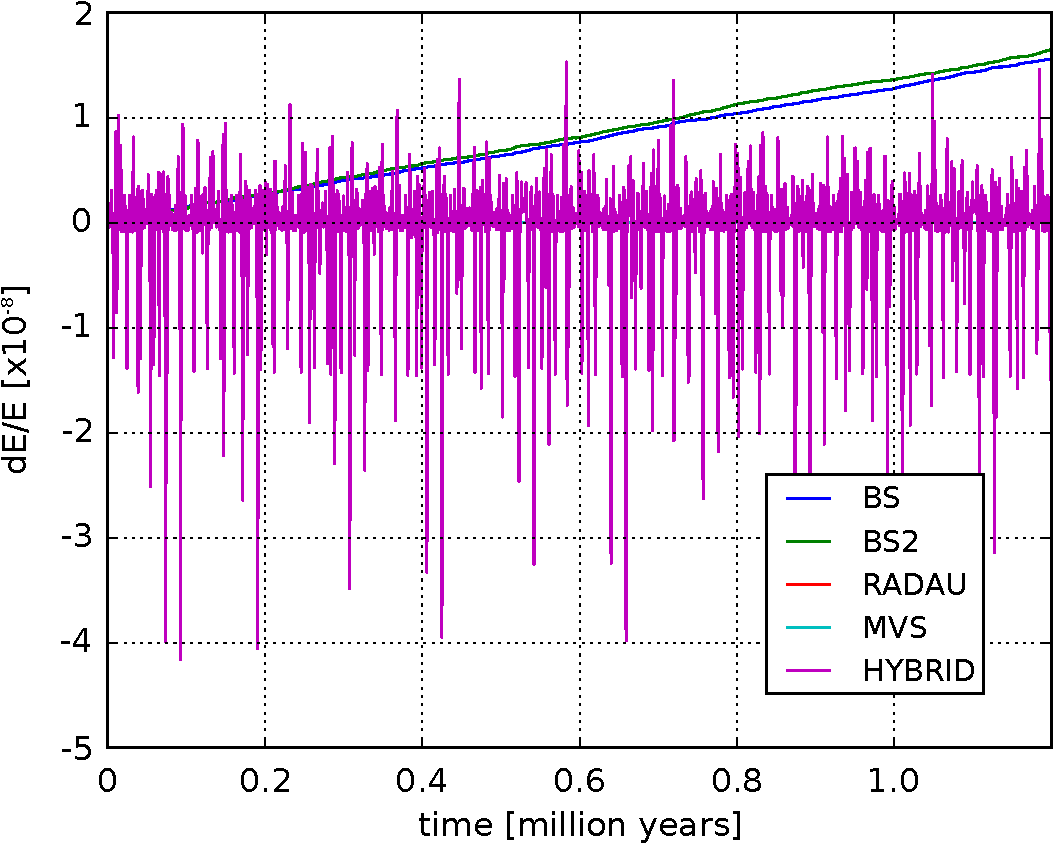
\includegraphics[width=0.65\linewidth]{figure/energy_error.pdf}
\caption[Pour une même simulation, erreur au cours du temps pour BS, BS2, RADAU, MVS et HYBRID.]{Évolution de l'erreur au cours
du temps pour une simulation contenant trois planètes d'une masse terrestre chacune, cette simulation étant lancée
successivement avec chacun des algorithmes disponibles dans \textbf{Mercury}. Les lignes correspondant 
aux intégrateurs MVS et RADAU sont superposées et confondues avec la ligne $\dif E/E=0$.}\label{fig:energy_error}
\end{figure}

Les algorithmes symplectiques ont cependant un inconvénient. Le pas de temps fixe d'un intégrateur symplectique ne permet pas de résoudre correctement les rencontres proches entre les corps du système. Chaque fois que le pas de temps d'un algorithme symplectique est changé, son hamiltonien change aussi, et entraine une variation d'énergie du système (dont l'énergie va osciller autour d'une nouvelle valeur moyenne). 

\bigskip

Nous cherchons maintenant à déterminer l'algorithme le plus approprié pour notre étude. Nous souhaitons faire évoluer un système avec plusieurs dizaines d'embryons planétaires pour plusieurs millions d'années, le système n'étant pas conservatif à cause des divers effets du disque que nous implémentons. 

Nous souhaitons résoudre correctement les orbites, mais avoir un temps de calcul raisonnable. 

La première contrainte est la dissipation. En effet, notre système n'est pas conservatif. Tous les algorithmes N-corps disponibles (BS, BS2 et RADAU) ne fonctionnent donc pas correctement, ces derniers réclament un pas de temps extrêmement faible qui n'est pas représentatif de la précision demandée pour l'intégration N-corps, la variation d'énergie numérique étant masquée par la variation d'énergie induite par les effets du disque. 

Il nous reste les algorithmes MVS et HYBRID. La deuxième contrainte, ce sont les rencontres proches et les collisions. Nous savons qu'un algorithme symplectique ne les traite pas correctement, et si c'est une erreur négligeable dans le cas où il y en a peu, ça ne l'est absolument plus dans notre cas, le nombre de rencontres proches pouvant être très important, notamment dans la phrase d'accrétion en début de simulation. L'algorithme MVS ne parait donc pas adapté contrairement à HYBRID qui a été construit pour être à la fois symplectique et gérer correctement les rencontres proches moyennant une erreur plus importante lors du changement d'algorithme. 

L'algorithme HYBRID est l'algorithme MVS, à pas de temps constant la majorité du temps. Il a donc les avantages d'un algorithme symplectique, à savoir la conservation de l'énergie et la rapidité d'exécution. Lors de rencontres proches (déterminées par une distance minimale d'approche entre deux corps, soit en rayon de Hill, soit en nombre de pas de temps), l'algorithme BS2 est utilisé, le pas de temps devient donc variable afin de résoudre correctement la rencontre et éventuellement la collision. Une fois fini, c'est de nouveau MVS qui prend le relai \citep[voir aussi ][]{mcneil2009new}. 

Dans notre cas, plusieurs approximations sont faites : 
\begin{itemize}
\item L'algorithme BS2 ne fonctionne que pour les systèmes conservatifs. On suppose que la variation d'énergie induite par la migration est totalement négligeable pendant le bref laps de temps de la rencontre proche
\item Le nombre de rencontres proches est suffisamment faible pour que les propriétés symplectiques de l'intégrateur soient 
conservées. On suppose de plus que les variations d'énergies induites par ce biais sont négligeables devant la dissipation 
induite par le disque (qui est de l'ordre de l'énergie initiale du système planétaire)
\end{itemize}

Il reste alors une chose à déterminer, c'est le pas de temps fixe que l'on doit choisir afin de résoudre correctement les orbites. Pour cela, on se place dans un cas simplifié, sans les effets du disque, et on souhaite savoir la condition sur le pas de temps afin que l'orbite soit correctement calculée. 

On ne s'intéresse qu'aux orbites internes qui sont limitantes au niveau du pas de temps en raison de leur période réduite. Pour une planète à une distance de $0.1\unit{UA}$ du soleil, la période orbitale est de 11 jours environ.

On réalise deux tests. Dans le premier test, on fait évoluer une planète de $1\mearth$ totalement isolée. On fait varier son demi-grand axe et son excentricité et on regarde comment évolue la conservation de l'énergie. Étant donné qu'avec un algorithme symplectique l'énergie oscille au cours du temps, on prend la valeur moyenne de la variation d'énergie, moyenne effectuée sur une centaine de valeurs.

Dans un deuxième test, on procède exactement de la même manière, à ceci près qu'on place une planète de $1\unit{M_\text{jup}}$ à $5\unit{UA}$. 

\reffig{fig:accuracy_maps} montre l'évolution de la conservation de l'énergie dans ces deux tests pour deux pas de temps différents, $h=1\unit{jour}$ et $h=0.4\unit{jour}$. Pour un pas de temps donné, nous ne pouvons pas donner simplement de position en dessous de laquelle l'orbite n'est pas correctement résolue. L'excentricité a une influence. En effet, la distance minimale entre l'étoile et la planète se situe au périhélie, mais suivant l'excentricité, la planète passera plus ou moins de temps au périastre. Ainsi, une très grande excentricité va diminuer drastiquement le temps passé au périastre, pour un périastre donné \citep{rauch1999dynamical, levison2000symplectically}. 

\begin{figure}[htbp]
\centering
\subfloat[$h=1\unit{jour}$ sans Jupiter]{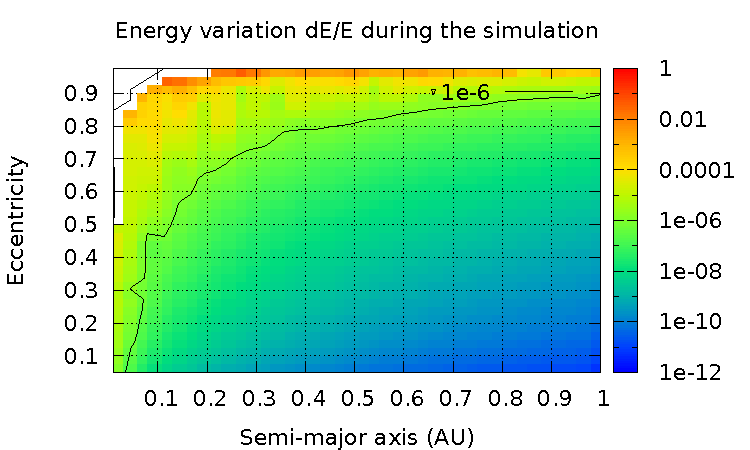
\includegraphics[width=0.49\textwidth]{figure/accuracy_10_one.pdf}}\hfill
\subfloat[$h=1\unit{jour}$ avec Jupiter]{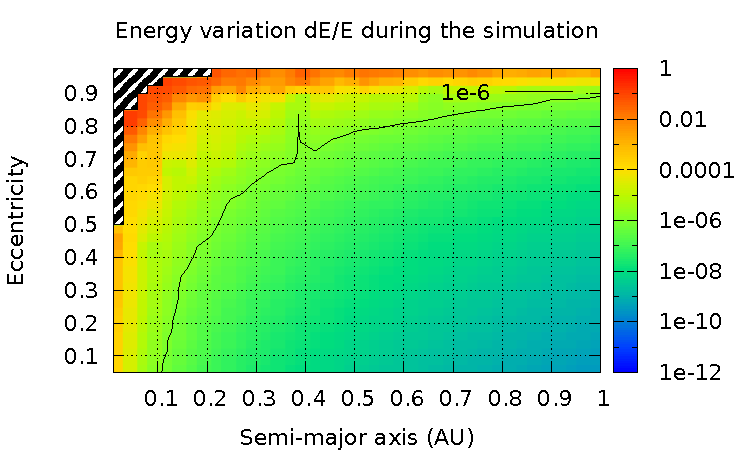
\includegraphics[width=0.49\textwidth]{%
figure/accuracy_10_jup.pdf}}

\subfloat[$h=0.4\unit{jour}$ sans Jupiter]{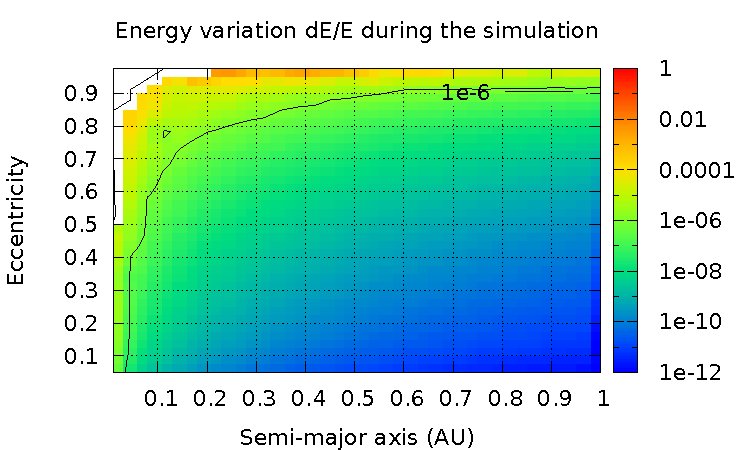
\includegraphics[width=0.49\textwidth]{figure/accuracy_04_one.pdf}}\hfill
\subfloat[$h=0.4\unit{jour}$ avec Jupiter]{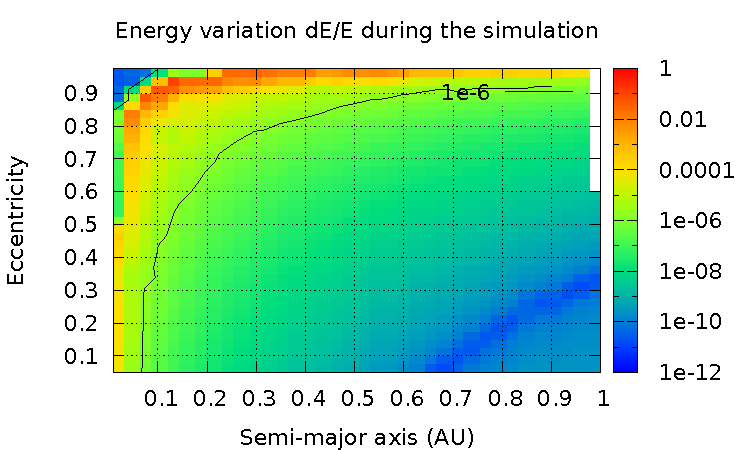
\includegraphics[width=0.49\textwidth]{%
figure/accuracy_04_jup.pdf}}


\caption[Conservation de l'énergie en fonction du pas de temps et des conditions initiales.]{Tests pour $h=1\unit{jour}$ et
$h=0.4\unit{jour}$ de la conservation de l'énergie pour une planète de $1\mearth$ isolée ou avec un compagnon de la taille de
Jupiter. Les cartes montrent la conservation de l'énergie pour différentes valeurs du demi-grand axe $a$ et de l'excentricité
$e$. La ligne noire correspond à un $\dif E/E=10^{-6}$, valeur en dessous de laquelle on considère que la précision sur l'orbite
est suffisante. La partie hachurée correspond à la collision de la planète interne avec l'étoile centrale donc le rayon est
$R_\star=0.005\unit{UA}$.}\label{fig:accuracy_maps}
\end{figure}

Si un pas de temps plus grand ($h=1\unit{jour}$) semble convenir pour une planète isolée, la conservation de l'énergie est
différente dans le cas avec des perturbations gravitationnelles (cas avec Jupiter). À $0.1\unit{UA}$, qui correspond au bord
interne, zone particulièrement importante pour notre étude, ce pas de temps ne convient plus. Dès que l'excentricité augmente un
peu, la précision sur l'orbite diminue, et les orbites les plus internes ne sont pas correctement résolues.

Même si le disque amortit les excentricités, nous souhaitons résoudre correctement les orbites légèrement excentriques, même au bord interne à $0.1\unit{UA}$. Un pas de temps de $h=1\unit{jour}$ résout correctement les orbites au bord interne, même légèrement excentriques, mais uniquement dans le cas d'une planète isolée. Si on ajoute les perturbations d'une planète externe, les orbites au bord interne ne sont plus correctement résolues. Ce défaut est corrigé si nous prenons un pas de temps de $h=0.4\unit{jour}$. C'est donc celui que nous utiliserons par défaut.

Un moyen mnémotechnique pour calculer le pas de temps minimal pour une simulation est de considérer qu'il faut résoudre l'orbite la plus proche avec un minimum de $10$ pas de temps. Ceci n'est valable que dans l'approximation où l'excentricité n'est pas trop élevée ($e<0.4$). Si nous faisons ce calcul ici, nous obtenons qu'avec un demi-grand axe minimal de $a=0.1\unit{UA}$ et une excentricité maximale de $e=0.4$, la distance minimale d'approche est $q=0.06$. La période d'une orbite $a=0.06$ est de $5\unit{jours}$ environ, ce qui donne un pas de temps maximal de $h=0.5\unit{jour}$. 

\section{Disque (1+1)D}
Afin de calculer les effets d'un disque de gaz, une modélisation de ce dernier est nécessaire. Le but étant d'avoir une grande
souplesse, le disque implémenté est bien entendu très simplifié. Toutes les quantités sont intégrées selon la hauteur $z$ et la
position azimutale $\theta$ dans le disque, résultant en un modèle radial 1D de toutes les quantités. Le nombre de points de
tous les profils est identique pour une même simulation. Typiquement le nombre de points égal à $n=1000$. Les points ne sont
pas régulièrement espacés, le nombre est plus important au bord interne de sorte que l'espacement $\Delta X$ entre les points
est constant, où $X$ est défini comme : 
\begin{align}
X = 2\sqrt{R}
\end{align}

Dans la mesure du possible, les quantités du disque ont été calculées de manière consistante. Je vais présenter dans la suite de manière chronologique comment sont calculées les grandeurs physiques du disque.

\subsection{Profil de densité de surface}
Le profil de densité de surface est défini au début de la simulation comme une loi de puissance de la forme :
\begin{align}
\Sigma(R) &= \Sigma_0 \times R^{-d}
\end{align}
où $\Sigma_0$ est la densité de surface à $1\unit{UA}$ et $d$ l'indice de la loi de puissance. 

Ce profil de densité de surface est défini pour une certaine étendue radiale. On définit donc un bord interne $R_\text{in}$ et un bord externe $R_\text{out}$. Le bord interne est généralement à $0.1\unit{UA}$ et le bord externe à $100\unit{UA}$. 

Afin de calculer les valeurs suivantes, ce disque est échantillonné et toutes les valeurs nécessaires sont ensuite calculées à chacun de ces points. 

\bigskip

Le profil de densité de surface est le paramètre d'entrée le plus important. Il est celui à partir duquel on calcule toutes les autres quantités du disque, température, échelle de hauteur, etc\dots

Le profil étant une loi de puissance, un amortissement est effectué au bord interne du disque afin que la valeur de la densité au bord interne soit proche de zéro. 

Le profil de densité de notre disque de référence (dont nous parlerons plus en détail \refsec{sec:migrations-maps}) est représenté \reffig{fig:fiducial_density}

\begin{figure}[htbp]
\centering
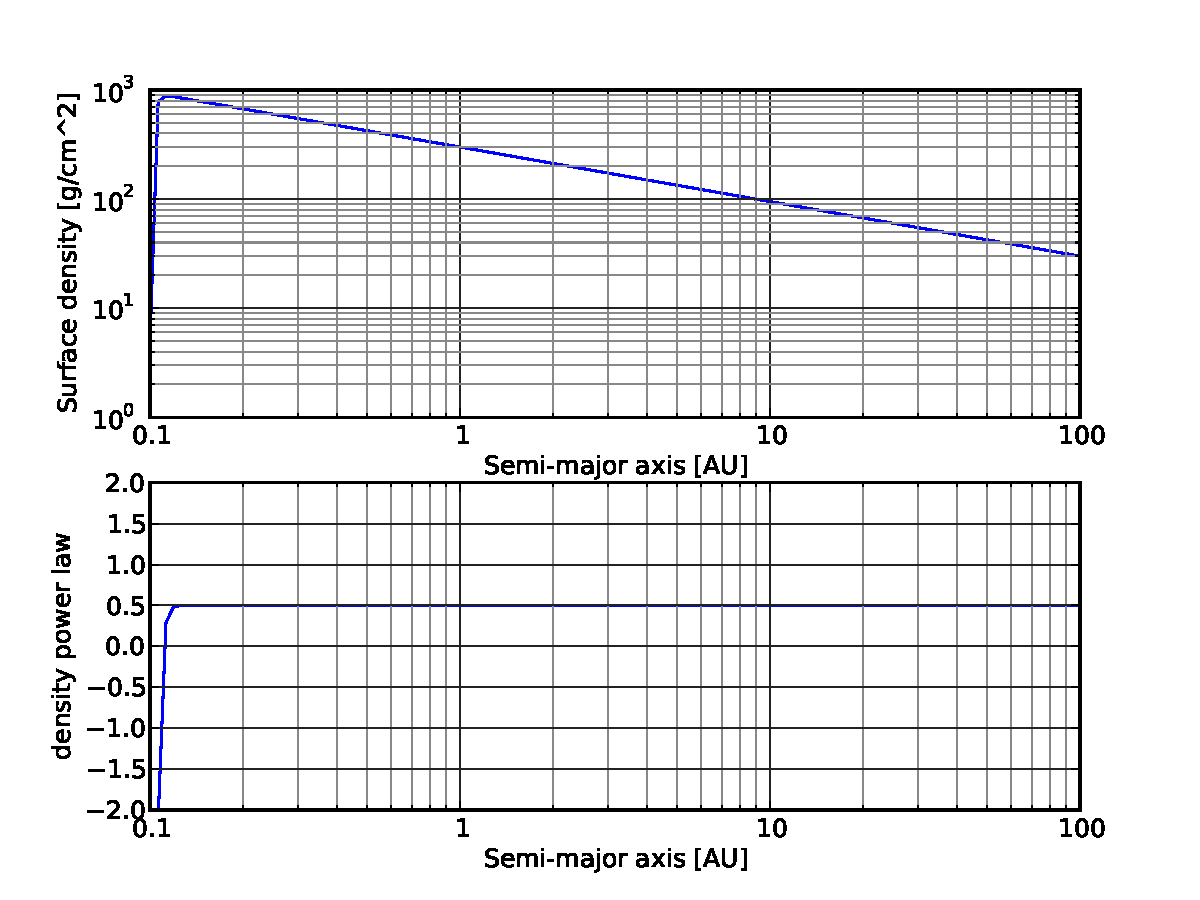
\includegraphics[width=0.75\linewidth]{figure/fiducial_density_profile.pdf}
\caption{Profil de densité de surface pour notre disque de référence \protect\reftab{tab:fiducial_parameters}.}\label{fig:fiducial_density}
\end{figure}

\subsection{Table d'opacité}\index{opacité}
Afin de pouvoir calculer le profil de température, on a besoin de choisir un modèle pour l'opacité. Je ne détaillerai pas ici les différents modèles car une étude spécifique a été menée \refsec{sec:influence_opacity_table} afin de comprendre l'influence du choix du modèle sur les résultats des simulations. 

Par contre, quel que soit le modèle, on a généralement une dépendance en fonction de la densité et de la température. L'opacité est donc un paramètre de la résolution de l'équation qui nous permet d'avoir la température. L'opacité n'est pas, dans notre modèle, une quantité qu'on fixe \emph{a priori}, mais plutôt un des paramètres de sortie de la résolution de l'équation de l'énergie dans le disque.

\subsection{Profil de température}
Afin de construire le profil de température point par point, on résout, pour chaque position dans le disque définie dans le profil, l'équation de l'énergie \refeq{eq:equation_energie}. 

De manière consistante, cette équation a pour paramètre d'entrée la position, et on cherche à trouver les valeurs de la température $T$, échelle de hauteur $H$, profondeur optique $\tau$, diffusivité thermique $\chi$. Toutes ces valeurs sont fixées une fois qu'un ensemble cohérent de valeurs satisfont l'équation.

Afin de résoudre cette équation du type $f(x)=0$, j'ai utilisé une version modifiée de la routine \textbf{zbrent} de \textbf{Numerical Recipes} \citep{press1992numerical}. Cette routine utilise la méthode de Van Wijngaarden-Dekker-Brent. Cette méthode est une combinaison de plusieurs méthodes et permet d'assurer la convergence tout en étant relativement rapide.

Le profil de température que nous obtenons dans notre disque de référence (dont nous parlerons plus en détail \refsec{sec:migrations-maps}) est représenté \reffig{fig:fiducial_temperature}

\begin{figure}[htbp]
\centering
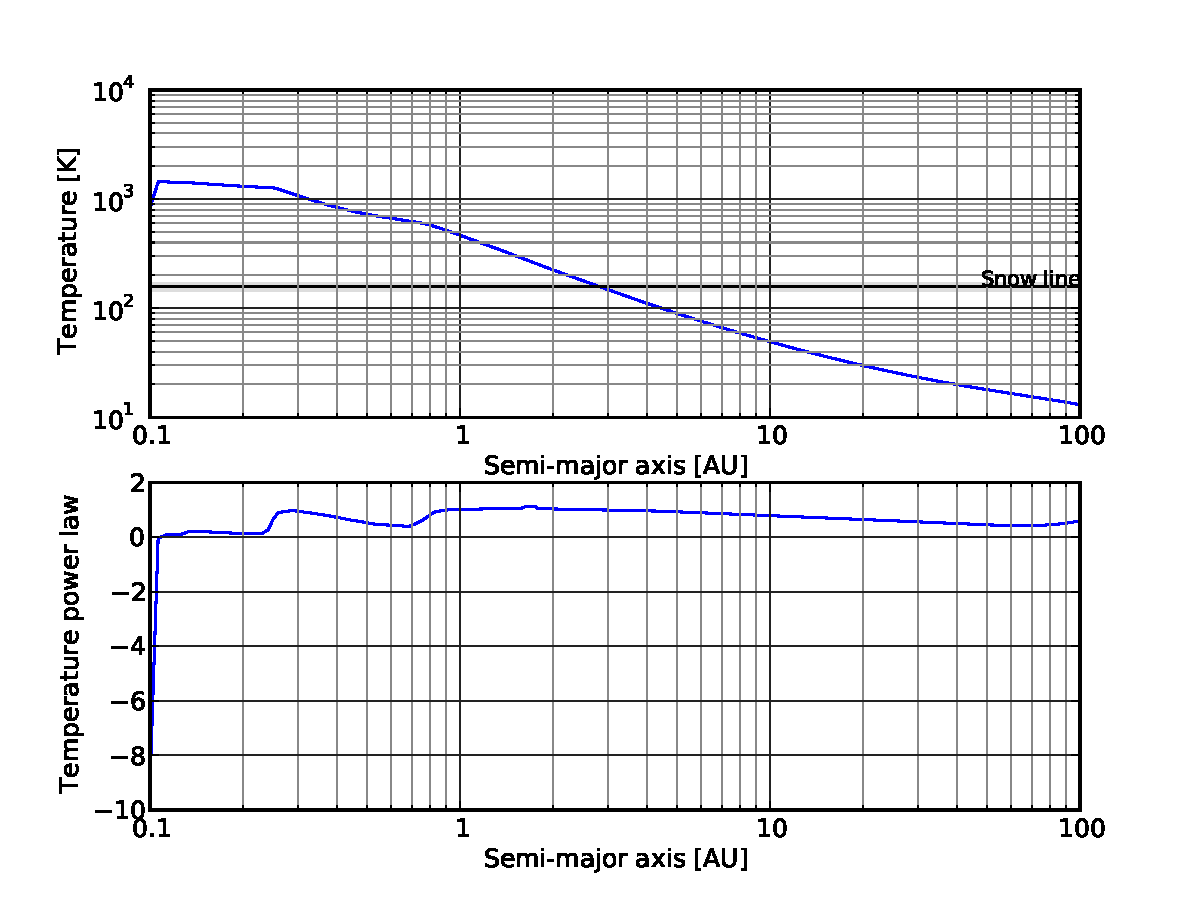
\includegraphics[width=0.75\linewidth]{figure/fiducial_temperature_profile.pdf}
\caption{Profil de température pour notre disque de référence \protect\reftab{tab:fiducial_parameters}.}\label{fig:fiducial_temperature}
\end{figure}

\section{Migration de Type I}\index{migration!Type I}
La migration de Type I est implémentée dans le code en utilisant le modèle 1D de disque, qui définit pour toute position du 
disque, une température, une densité de surface, et tous les autres paramètres nécessaires comme l'échelle de hauteur. En 
utilisant ces paramètres, on obtient ainsi le couple qu'exerce le disque sur la planète en fonction de sa masse et de sa 
position via la formule semi-analytique de \cite{paardekooper2011torque}. Plus exactement, j'implémente les formules décrites 
\refsec{sec:type_I}, équations \refeq{eq:lindblad-torque}, \refeq{eq:saturated-corotation-torque} et 
\refeq{eq:linear-corotation-torque}. Ces formules sont une combinaison de \cite{paardekooper2010torque} où l'effet du paramètre 
de lissage $b/h$ apparaît de manière explicite, mais qui ne modélise que les couples linéaires, et \cite{paardekooper2011torque} 
où l'effet de la diffusion est pris en compte, mais où la longueur de lissage n'apparait pas explicitement. Ainsi, nous 
obtenons des formules pour la migration de Type I qui dépendent du paramètre de lissage $b/h$(\refeq{eq:lindblad-torque}, 
\refeq{eq:saturated-corotation-torque} et 
\refeq{eq:linear-corotation-torque}), et qui en plus tiennent compte 
de la saturation \citep[eqs. (50) à (53)]{paardekooper2011torque}.

Les deux différences principales entre le cadre du modèle de \cite{paardekooper2011torque} et le disque que j'ai modélisé, c'est que dans mon cas je n'ai pas un profil de température en loi de puissance (avec une seule loi de puissance), mais j'ai une loi de puissance définie point par point. C'est-à-dire que pour chaque zone du disque, la température est calculée de manière cohérente avec les autres paramètres du disque, et que l'indice de la loi de puissance correspondante est calculée en fonction des températures autour.

La deuxième différence est que j'ai un profil pour l'échelle de hauteur $H$ et le rapport d'aspect $h=H/R$ du disque au lieu d'avoir un rapport d'aspect constant pour tout le disque.

\bigskip

De plus, certaines erreurs se sont glissées dans ce papier. \cite[appendice A]{bitsch2011range} fait remarquer en particulier qu'il manque un facteur 4 dans l'équation (33). Ainsi, la formule que j'ai utilisé pour calculer la conductivité thermique $\chi$ est :
\begin{align}
\chi &= \frac{16\gamma (\gamma-1) \sigma T^4}{3\kappa \rho^2 H^2\Omega^2}
\end{align}

Il y a aussi une erreur dans l'équation (35) car le disque se refroidit par la surface supérieure et la surface inférieure. Mais comme j'utilise dans mon code une équation de l'énergie \refeq{eq:equation_energie} un peu plus complexe où j'ai tenu compte de ce fait là, cette erreur n'a pas d'incidence sur le calcul du couple.

Les formules nous donnent alors un couple exercé par le disque sur la planète. 

À partir de ce couple, on définit un temps de migration $t_\text{mig}$ comme : 
\begin{align}
t_\text{mig} &= -\frac{J}{\Gamma}
\end{align}
où $J$ est le moment cinétique total de la planète et $\Gamma=\dot{J}$ est le couple total exercé par le disque sur la planète.

L'accélération due à la migration $\vect{a_\text{mig}}$ est alors donnée par\citep[eq. 
(14)]{cresswell2008three} :
\begin{align}
\vect{a_\text{mig}} &= -\frac{\vect{v}}{t_\text{mig}}
\end{align}
où $\vect{v}$ est la vitesse instantanée de la planète.

\section{Amortissement de e et I}
L'amortissement de l'excentricité $e$ et de l'inclinaison $I$ d'une planète plongée dans un disque protoplanétaire est modélisé
dans le code via les formules de \cite[eq. (9), (11) et (12)]{cresswell2008three} : 
\begin{subequations}
\begin{align}
t_e &= \frac{t_\text{wave}}{0.780}\left[1-0.14\left(\frac{e}{H/r}\right)^2 + 0.06 \left(\frac{e}{H/r}\right)^3 + 0.18\left(\frac{e}{H/r}\right)\left(\frac{I}{H/r}\right)^2\right]\\
t_I &= \frac{t_\text{wave}}{0.544}\left[1-0.30\left(\frac{I}{H/r}\right)^2 + 0.24 \left(\frac{I}{H/r}\right)^3 + 0.14\left(\frac{e}{H/r}\right)^2\left(\frac{I}{H/r}\right)\right]\\
t_\text{wave} &= \frac{M_\star}{m_p}\frac{M_\star}{\Sigma_p {a_p}^2}\left(\frac{H}{r}\right)^4{\Omega_p}^{-1}
\end{align}
\end{subequations}

L'amortissement de $I$ est arrêté quand l'inclinaison descend en dessous de $I<5\cdot 10^{-4}\unit{rad}$ afin d'empêcher les planètes d'être parfaitement dans le plan $(x,y)$, essentiellement pour empêcher des problèmes numériques.

\section{Effet de l'excentricité sur le couple de corotation}\index{amortissement!couple de corotation}
Afin de tenir compte d'un effet mis en évidence par \cite{bitsch2010orbital}, une petite modification a été effectuée dans le calcul du couple total $\Gamma$ exercé par le disque sur la planète. 

En effet, il a été montré que l'excentricité d'une planète a une influence sur sa zone fer-à-cheval et par extension, sur son couple de corotation $\Gamma_C$. Un paramètre d'amortissement $D$, compris entre 0 et 1 a ainsi été ajouté au calcul du couple total \citep{hellary2012global} :
\begin{align}
\Gamma &= \Gamma_0 \cdot (\frac{\Gamma_L}{\Gamma_0} + D\cdot \frac{\Gamma_C}{\Gamma_0})
\end{align}
où $\Gamma_0 = \left(\frac{q}{h}\right)^2\Sigma_p {r_p}^4 {\Omega_p}^2$ et $\Gamma_L$ est le couple de Lindblad.

La valeur du paramètre d'amortissement $D$ est donnée par une formule qui a été calculée pour coller au mieux aux simulations de \cite{bitsch2010orbital}, détaillée dans \cite{cossou2013convergence}, et recopiée ici : 
\begin{subequations}
\begin{align}
D = \frac{\Gamma_C(e)}{\Gamma_C (e=0)} &= 1 + a \cdot \left[\tanh(c) - \tanh\left(\frac{b * e}{x_s}+c\right)\right]\label{eq:eccentricity-influence}\\
a &= 0.45 \qquad b=3.46 \qquad c= -2.34
\end{align}
\end{subequations}
où $x_s$ représente la demi-largeur de la région fer-à-cheval adimensionnée.

\section{Désactivation des effets du disque}
Quand une planète sort des bornes du disque, les effets d'amortissement de $e$ et $I$ sont désactivés, au même titre que la migration due à la présence du disque. Ce cas survient rarement au bord externe du disque (généralement à $100\unit{UA}$), mais est beaucoup plus probable au bord interne (généralement à $0.1\unit{UA}$).

\section{Validité des éléments orbitaux}
Lors d'une rencontre proche entre deux planètes, leurs interactions gravitationnelles rendent caduques les formules qui permettent de calculer les éléments orbitaux à partir des vitesses et positions car ceci suppose qu'on est dans le cas d'une orbite képlerienne isolée. 

Dans de tels cas, on peut avoir des demi-grands axes négatifs, des excentricités supérieures à 1. Si c'est déjà en soit un 
problème physique, c'est aussi et surtout un problème numérique car cela fait apparaître des \textbf{Not A Number} (NaN) lorsque 
par exemple le demi-grand axe est en argument d'une racine carrée. Ceci a donc pour conséquence concrète de faire planter le 
code, au mieux, ou pire, de le faire tourner avec tous les paramètres de la simulation peu à peu gangrénés par des 
\textbf{NaN}. 

Dans un premier temps, j'ai pensé remplacer dans mes calculs le demi-grand axe par le rayon $r=\sqrt{x^2+y^2+z^2}$, afin 
d'éviter les problèmes lors des rencontres proches. Cette solution fait apparaître d'autres problèmes, notamment avec des 
orbites excentriques proches du bord interne. Dans ce cas, on peut avoir une planète qui ressent un couple positif au bord 
interne, puis plus de couple du tout dans la partie de l'orbite qui sort du disque, et enfin un couple négatif quand la planète 
est dans le disque, mais hors du bord interne. Ceci cause de gros problèmes et génère des orbites qui ne sont pas physiques 
mais dues à une astuce qui cherche à contourner un problème numérique. En effet, les formules de migration sont moyennées sur 
une orbite, on ne peut donc pas avoir de telles variations au sein d'une même orbite.

La solution adoptée est de tester les cas qui causent des NaN, c'est à dire typiquement des excentricités supérieures à 1, et 
un demi-grand axe négatif. Quand de tels cas surviennent, on désactive momentanément la migration et tous les effets du 
disque. Le reste du temps, la migration est systématiquement calculée, y compris pendant les rencontres proches. On considère 
que le temps durant lequel le calcul des éléments orbitaux n'est plus valide représente un temps négligeable de la 
simulation au regard des centaines de milliers d'années sur lesquelles on intègre les orbites. On considère donc que la 
migration induite sur les planètes pendant les rencontres proches est totalement négligeable au regard du reste de la 
simulation.



\chapter{Cartes de migration}\label{sec:chap3}
Dans les disques isothermes, la migration de Type I est gouvernée par le couple différentiel de Lindblad et le couple de corotation, qui induisent généralement
une migration vers l'intérieur \citep{goldreich1980disk, ward1986density, tanaka2002three}. Dans les disques radiatifs, un terme supplémentaire du couple de corotation provenant d'un gradient d'entropie peut contrebalancer le couple
différentiel de Lindblad sous certaines conditions et ainsi inverser le sens de migration (vers l'extérieur)
\citep{paardekooper2006halting, kley2008migration}. Il est donc possible d'avoir dans un disque des zones où la migration
s'arrête. Ces zones sont appelées zone de convergence \citep[CZs;][]{lyra2010orbital,
paardekooper2011torque, hellary2012global}. 

\bigskip

À la zone de convergence, le couple de corotation (positif) compense exactement le couple différentiel de Lindblad (négatif).
Ainsi, à la zone de convergence, une planète ne migre pas.

De plus, autour de la zone de convergence, la migration tend à ramener les embryons vers la zone de couple nul s'ils s'en
éloignent. La zone de convergence est donc une position stable dans le disque vers laquelle les embryons se rassemblent.

De même, il peut exister des zones de couples nuls qui ne sont pas des zones de convergence quand, en s'éloignant légèrement, la
migration tend à les éloigner davantage. Ces zones sont alors instables.

Les zones de convergence pourraient ainsi concentrer les embryons planétaires et être le lieu de formation de planètes (ou
cœurs) massives \citep{lyra2010orbital, horn2012orbital}. 

\bigskip

Je vais montrer dans les paragraphes qui suivent que la migration est extrêmement sensible aux paramètres du disque.

\cite{kretke2012importance} ont étudié l'influence des paramètres du disque sur la migration. Cependant, s'ils ont inclus des
effets fins sur le bord interne et la migration, la dépendance de l'opacité en fonction de la température et de la densité est
approximée par différentes lois de puissance. Nous montrerons que l'opacité est un paramètre sensible du modèle et qu'il est
important de la modéliser le plus finement possible. 

\cite{bitsch2013influence} ont étudié en particulier l'effet de la viscosité $\nu$ et l'indice adiabatique $\gamma$ sur la
migration dans le disque, au travers de simulations 3D. 

Afin d'étudier séparément l'effet des paramètres du disque, j'ai choisi un disque de référence, décrit
\refsec{sec:migrations-maps}. Dans cette partie, je présente les cartes de migration et comment les interpréter. En particulier
je présente la carte de migration du disque de référence \reffig{fig:fiducial_migration_map}. Pour chaque paramètre, je vais
donc conserver les valeurs du disque de référence, et faire varier le paramètre en question autour de la valeur de référence. Sauf
mention contraire, un seul paramètre est donc modifié à la fois, seuls les paramètres qui changent sont précisés, les autres
sont regroupés \reftab{tab:fiducial_parameters}.

\section{Disque de référence}\label{sec:migrations-maps}\label{sec:reference_disk}

\begin{figure}[htbp]
\centering
\subfloat[Couple Adimensionné]{\label{fig:fiducial_adim}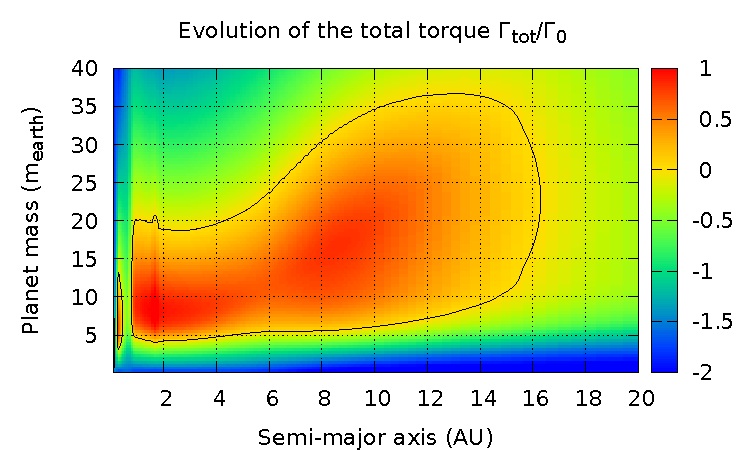
\includegraphics[width=0.49\textwidth]{figure/migration_map/fiducial.pdf}}\hfill
\subfloat[Couple Réel]{\label{fig:fiducial_units}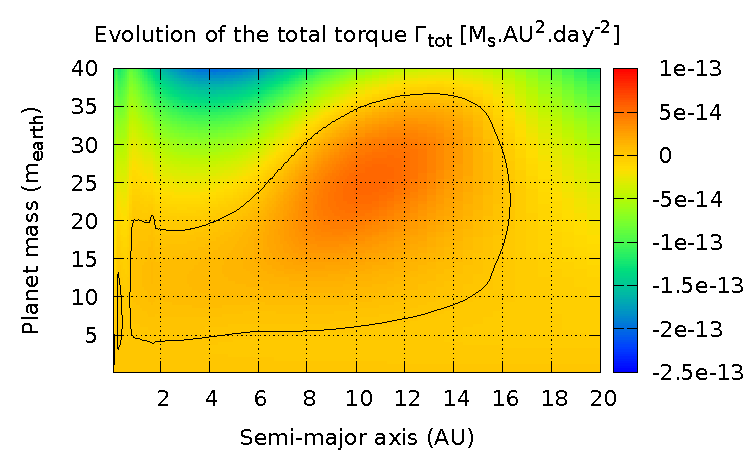
\includegraphics[width=0.49\textwidth]{%
figure/migration_map/fiducial_units.pdf}}

\caption[Carte de migration pour le disque de référence.]{Carte de migration pour le disque de référence. Cette carte montre le
sens de migration d'une planète en fonction de sa
position (abscisse) et de sa masse (ordonnée). La 3\ieme coordonnée est le couple total exercé par le disque sur la planète,
exprimé en unité de $\Gamma_0 = \left(\frac{q}{h}\right)^2\Sigma_p {r_p}^4 {\Omega_p}^2$ pour la carte de gauche, et en \unit{M_\odot UA^2/jour^2} pour la carte de droite. Quand le couple est positif (resp.
négatif), la migration est vers l'extérieur (resp. intérieur). La ligne noire représente la zone de couple nul, où la planète ne
migre plus. Des masses jusqu'à $40\mearth$ sont affichées, dans l'unique but d'afficher des contours fermés. Il est probable 
qu'à de telles masses, une cavité s'ouvre autour de la planète, limitant la validité des formules de migration de Type I 
implémentés ici \citep{paardekooper2011torque}. Le détail des paramètres du disque de référence est donné 
\reftab{tab:fiducial_parameters}.
}\label{fig:fiducial_migration_map}
\end{figure}

Dans cette partie, nous allons présenter notre disque de référence et comment ses paramètres vont influencer la migration des
planètes. Ce disque de référence servira aussi de comparaison quand nous étudierons les effets des paramètres du disque.

Ce disque est obtenu à l'aide de la table d'opacité d'\cite{hure2000transition}. Le profil de température est
calculé en tenant compte de l'irradiation, avec des paramètres solaires pour la température et le rayon de l'étoile ($T_\star =
5700\unit{K}$ ; $R_\star = 4.65\cdot 10^{-3}\unit{UA}$). L'albédo du disque est pris égal à $0.5$. La viscosité est calculée à
partir d'une prescription alpha \citep{shakura1973black}. On considère un disque dont les bords internes et externes sont
respectivement à $0.1$ et $100\unit{UA}$. Les autres paramètres du disque sont récapitulés \reftab{tab:fiducial_parameters}. 

\begin{table}[htbp]
\centering
\begin{tabular}{|c|c|c|c|}
\hline
$b/h = 0.4$ & $\gamma = 7/5$ & $\mu = 2.35$ & $\alpha = 5\cdot 10^{-3}$ \\\hline
\multicolumn{2}{|c|}{Inner edge : $0.1\unit{UA}$} & \multicolumn{2}{c|}{Outer edge : $100\unit{UA}$}\\\hline
\multicolumn{2}{|c|}{$\Sigma(R) = 300 \cdot (R/1\unit{AU})^{-1/2}\unit{g/cm^2}$}& \multicolumn{2}{c|}{$M_\text{tot} = 0.14\unit{M_\odot}$}\\\hline
$T_\star = 5700\unit{K}$ & $R_\star = 4.65\cdot 10^{-3}\unit{UA}$ & \multicolumn{2}{c|}{Disk albedo : $0.5$}\\\hline
\end{tabular}
\caption[Paramètres physiques du disque de référence.]{Paramètres physiques du disque de référence. Les opacités sont calculées
à partir de la table d'opacité de
\cite{hure2000transition}. La viscosité est calculée en suivant la prescription alpha de
\cite{shakura1973black}.}\label{tab:fiducial_parameters}
\end{table}

Le paramètre de lissage $b/h$ est pris assez faible afin de ne pas sous-estimer le couple de corotation, qui est la partie la plus importante du couple dans notre cas, car c'est celle qui permet d'inverser le sens de migration. En faisant cela, on surestime le couple de Lindblad, pour lequel un paramètre de lissage $b/h=0.75$ est conseillée \citep{masset2002coorbital}.
En considérant que le gaz du disque est un gaz parfait diatomique, l'indice adiabatique vaut alors $\gamma=7/5$.
La valeur de $\alpha$ correspond à une valeur typique observée. De plus, elle tient compte du fait que la viscosité diminue avec l'âge du disque et que nous considérons une époque où le disque a déjà évolué, puisque nous prenons des embryons relativement massifs (au minimum $0.1\mearth$). De même, le profil de densité de surface $\Sigma(R) = 300 \cdot R^{-1/2}\unit{g/cm^2}$ ne correspond pas à un disque très massif car on considère que le disque est déjà évolué. 

Afin d'étudier la migration dans les disques, il est pratique de 
regarder une \og carte de migration\fg, comme \reffig
{fig:fiducial_migration_map}. Cette carte permet de voir rapidement 
les parties intéressantes et de prédire l'évolution d'une planète à 
partir des positions et masses initiales. Le couple adimensionné 
\reffig{fig:fiducial_adim} sera préférentiellement utilisé quand 
nous représenterons une carte de migration ensuite, car plus intuitif 
à lire. La carte \reffig{fig:fiducial_units} montre que le couple 
total a des dépendances complexes au travers de $\Gamma_0$. Il 
dépend notamment de la masse de la planète, du rapport d'aspect et 
de la densité locale du disque. \reffig{fig:fiducial_migration_map} montre la carte de migration du disque de référence que nous utiliserons de manière
récurrente ici. 

\begin{figure}[htbp]
\centering
\subfloat[Lindblad torque]{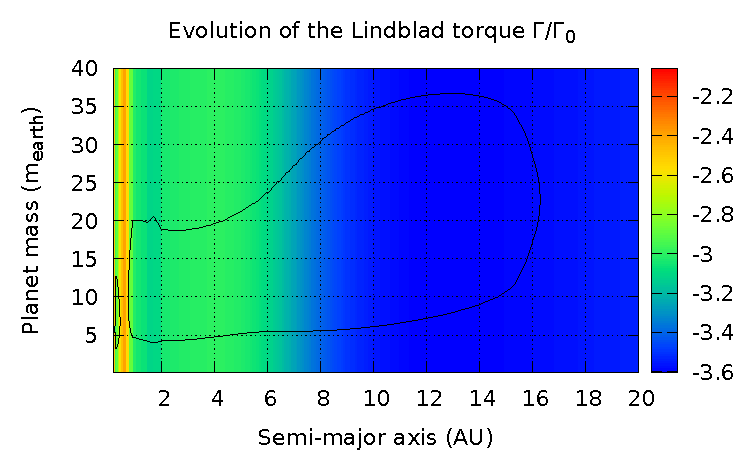
\includegraphics[width=0.49\textwidth]{figure/migration_map/details/lindblad_torque.pdf}}\hfill
\subfloat[Entropy-related horseshoe drag]{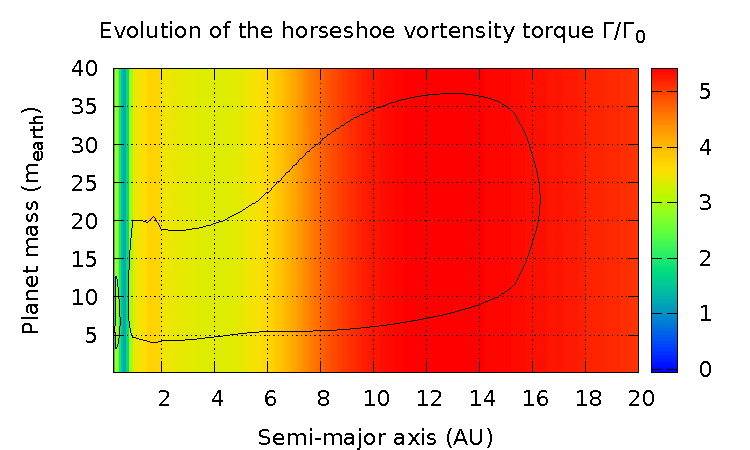
\includegraphics[width=0.49\textwidth]{%
figure/migration_map/details/ent_hs_torque.pdf}}

\caption[Carte des couples de Linblad et corotation.]{Évolution des deux couples les plus importants vis-à-vis de la carte de
migration, le couple de Lindblad et la partie
non-saturée du couple de corotation liée au gradient d'entropie. En effet, ces deux couples sont quantitativement plus grands que
tous les autres. Ici, seule la partie non-saturée du couple de corotation est représentée.}\label{fig:details_maps}
\end{figure}

Sur \reffig{fig:details_maps} sont représentés les deux couples les plus importants en terme d'amplitude. D'une part le couple négatif dominant, le
couple de Lindblad $\Gamma_L$, et d'autre part le couple positif dominant, la partie du couple de corotation non saturée liée au gradient d'entropie
$\Gamma_\text{ent,hs}$. Ici, c'est bien la partie non saturée qui est représentée (fully unsaturated horseshoe drag en anglais). On ne tient pas
compte de la diffusion. On constate alors que sans tenir compte de la diffusion, les couples sont totalement indépendants de la
masse. La transition que l'on constate dans les deux cartes, entre $6-8\unit{UA}$ correspond à la transition disque
actif/passif. L'irradiation est le processus de chauffage principal à partir de $5\unit{UA}$ comme illustré par
\reffig{fig:viscous_vs_irradiation}.

\begin{figure}[htbp]
\centering
\subfloat[$t_\text{rad}/t_\text{U-turn}$]{\label{fig:linear_rad}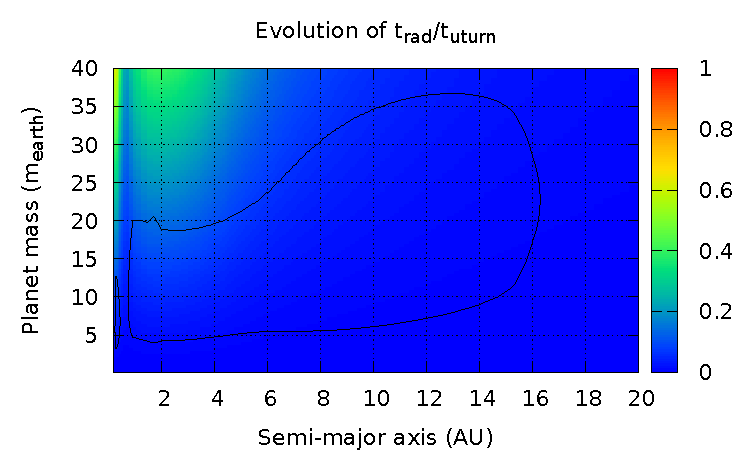
\includegraphics[width=0.49\textwidth]{%
figure/timescales/linear_rad.pdf}}\hfill
\subfloat[Saturation : $(t_\text{lib}/2)/t_\text{visc}$]{\label{fig:sat_visc}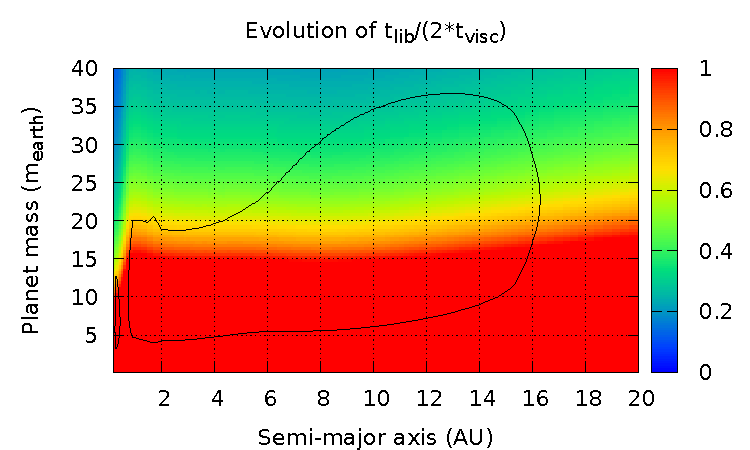
\includegraphics[width=0.49\textwidth]{%
figure/timescales/sat_visc.pdf}}

\caption[Cartes des temps de diffusions dans le disque.]{Comparaison des différents temps caractéristiques influençant le couple
de corotation. Ces inéquations sont détaillées
dans \refsec{sec:couple-corotation}. Dans le cas présent, le temps de diffusion radiative est toujours plus court que le temps
de diffusion visqueuse, $t_\text{rad}<t_\text{visc}$. Ainsi, il ne reste plus que les deux inégalités représentées
ici. La saturation est ainsi gouvernée par le temps de diffusion visqueuse $t_\text{visc}$. La transition couple non-saturé/couple linéaire est elle déterminée par le temps de diffusion radiative $t_\text{rad}$.}\label{fig:timescales_maps}
\end{figure}

\reffig{fig:timescales_maps} représente l'effet de la diffusion sur la carte de migration. Dans le cas d'un disque purement actif, on s'attend à ce que $t_\text{rad}=t_\text{visc}$ car $\nu\propto\xi$. Ici, à cause de l'irradiation, nous avons $t_\text{rad}<t_\text{visc}$, la saturation est alors gouvernée par le temps de diffusion visqueuse $t_\text{visc}$ et la transition couple non-saturé/couple linéaire est déterminée par le temps de diffusion radiative $t_\text{rad}$. Ainsi, seules deux inégalités sont ici nécessaires pour étudier le couple de corotation :
\begin{align}
t_\text{U-turn} < t_\text{diff} < \frac{t_\text{lib}}{2}\\\nonumber
t_\text{U-turn} < t_\text{rad} < t_\text{visc} < \frac{t_\text{lib}}{2}
\end{align}

Sur \reffig{fig:timescales_maps} on remarque que les parties active et passive du disque sont distinctes. En dessous de $4\unit{UA}$, la partie supérieure de la carte de migration s'explique par la saturation du couple de corotation. La ligne de couple nul suit en effet l'équation $(t_\text{lib}/2) = t_\text{visc}$ \reffig{fig:sat_visc}.

La partie inférieure quant à elle, s'explique par la transition entre le couple non saturé et le couple linéaire pour le couple de corotation. La ligne de couple nul suit en effet l'équation $t_\text{U-turn} = t_\text{rad}$ \reffig{fig:linear_rad}. Le couple de corotation devient linéaire quand le temps de diffusion radiative est trop court pour permettre à un gradient de s'installer dans la zone fer-à-cheval.

\begin{figure}[htbp]
\centering
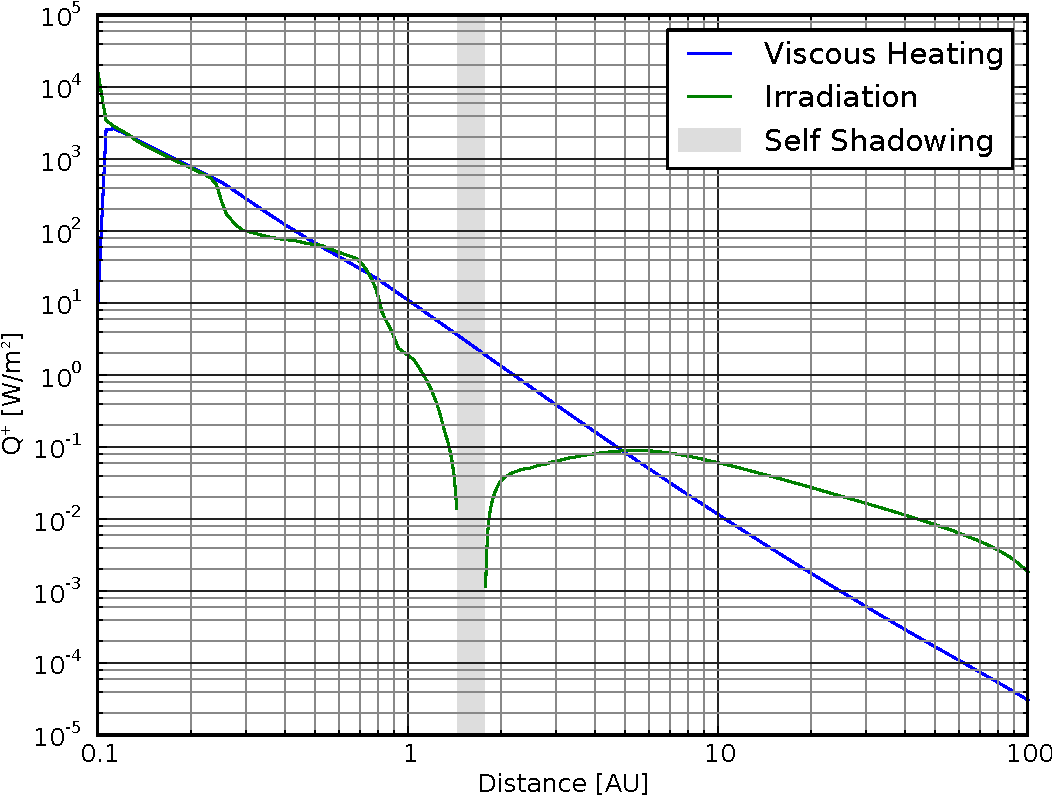
\includegraphics[width=0.75\textwidth]{figure/migration_map/viscous_vs_irradiation.pdf}

\caption[Amplitude du chauffage visqueux et de l'irradiation dans le disque.]{Amplitude des termes sources dans l'équation
d'énergie liés au chauffage visqueux et à l'irradiation. Dans les parties internes, c'est le
chauffage visqueux qui domine, dans les parties externes c'est l'irradiation. À $5\unit{UA}$ les deux contributions sont
égales. La partie grisée correspond à la zone où l'irradiation est forcée à 0 car l'angle d'interception des rayons solaires est négatif (l'échelle de hauteur diminue). Ce n'est donc pas à proprement parler un \og Self-Shadowing\fg qui concerne une zone beaucoup plus étendue.}\label{fig:viscous_vs_irradiation}
\end{figure}

À partir de $5\unit{UA}$, l'irradiation domine le bilan énergétique \reffig{fig:viscous_vs_irradiation} et une simple comparaison des temps de diffusion ne permet plus d'expliquer simplement l'allure de la carte de migration. Ce n'est plus seulement les temps de diffusion qui permettent de trouver la zone de couple nul dans le disque, mais les valeurs des couples eux-mêmes. Au delà de $4\unit{UA}$, sans tenir compte de la saturation les couples augmentent différemment. En effet, au delà de $4\unit{UA}$, le profil de température est dominé par l'irradiation et l'indice du gradient de température diminue avec la distance à partir de $d=1$ à $4\unit{UA}$ jusqu'à $d=0.5$ à $40\unit{UA}$. Les couples de Lindblad et de corotation n'ayant pas les mêmes dépendances vis-à-vis du gradient de température, l'écart entre les couples change.

La fermeture des parties externes de la carte de migration s'explique donc par l'action conjointe de la diffusion radiative et visqueuse. Pour les masses
faibles, en dessous de $15-20\mearth$, la migration vers l'intérieur est due au fait que $t_\text{U-turn} > t_\text{rad}$, c'est
alors la valeur linéaire du couple de corotation qui prévaut. Pour les masses plus importantes, le couple de corotation sature
car $(t_\text{lib}/2) < t_\text{visc}$. 

\bigskip

Avant $1\unit{UA}$, deux régions de couples positifs sont séparées par une région peu étendue où la migration est dirigée vers l'intérieur. C'est une transition d'opacité à $1\unit{UA}$ qui
en est la cause, et qui change brusquement les couples de migration \reffig{fig:details_maps}. Ce
brusque changement d'opacité et de température est la raison de la séparation de la zone de couple positif en deux. 

Nous avons alors deux zones de couple nul dont l'origine physique et les propriétés sont quelque peu différentes. 

\section{Différents types de zone de convergence}\label{sec:CZ-types}\index{zone de convergence}
À partir de ces cartes de migration nous pouvons étudier l'évolution des différentes zones de couple nul en fonction de la
distance. Ces zones sont représentées par une ligne noire. Nous pouvons dégager deux types particuliers de zones de convergence. 

Le premier type de zone de convergence est ce que nous appellerons une \textbf{zone de convergence indépendante de la masse}. C'est une
zone qui se trouve plutôt dans les parties internes du disque et est généralement créée par une transition d'opacité. Cette ligne de couple nul dépend très peu de la masse de la
planète car une transition d'opacité induit de brusques changements de température. Les couples varient ainsi fortement sur une
distance très courte. Cette zone de convergence a deux caractéristiques importantes : 
\begin{enumerate}
\item La position de la zone de convergence ne dépend pas ou peu de la masse de la planète
\item La variation du couple de migration autour de la zone de convergence est très forte
\end{enumerate}

Nous pouvons appeler le deuxième type \textbf{zone de convergence dépendante de la masse}. En effet, dans les parties externes, le
couple varie plus doucement en fonction de la distance. L'influence de la masse est donc plus marquée dans la position de la zone
de couple nul. Ce type de zone de convergence a deux caractéristiques importantes : 
\begin{enumerate}
\item La position de la zone de convergence dépend de la masse de la planète. 
\item Le couple de migration varie doucement en fonction de la distance à la zone de convergence
\end{enumerate}

\begin{figure}[htbp]
\centering
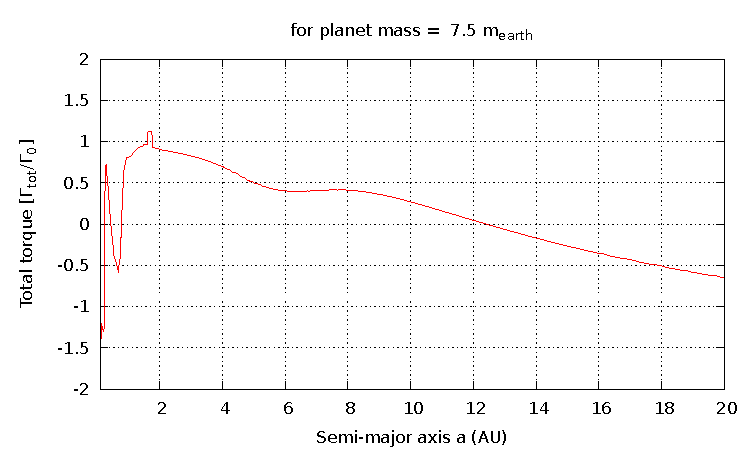
\includegraphics[width=0.75\linewidth]{figure/total_torque_fixed_m.pdf}
\caption{Évolution du couple total exercé par
le disque sur une planète de $7.5\mearth$. }\label{fig:total_torque_fixed_m}
\end{figure}

\reffig{fig:total_torque_fixed_m} illustre les deux zones de convergence. La première près de $1\unit{UA}$, siège d'une
variation brutale du couple de migration, et la deuxième (dont la position dépend de la masse de la planète) où la variation du
couple de migration est continue. 

Dans la suite, nous utiliserons parfois des zones de convergence artificielles afin de simplifier les effets, et d'étudier
plus facilement un phénomène particulier. Dans le cas d'une transition d'opacité, nous avons modélisé les zones de convergence
indépendantes de la masse par une fonction tangente hyperbolique dont le zéro se situe à la zone de convergence, et où le couple de
migration (positif ou négatif) sature très loin de la zone de convergence \refsec{sec:tanh_indep}. Pour modéliser une zone de
convergence indépendante de la masse où le couple varie peu autour de la zone de convergence, nous avons utilisé une variation
linéaire du couple de migration \refsec{sec:linear_indep}.

Les zones de convergence dépendantes de la masse peuvent être approximées par une variation linéaire de la position de la zone
de couple nul en fonction de la masse. Le couple de migration varie quant à lui linéairement en fonction de la distance
\refsec{sec:mass_dependant}. 

\bigskip

Il existe malgré tout un point commun aux zones de convergence, quel que soit leur type. Une planète doit être suffisamment massive pour migrer vers la zone de convergence. En dessous d'une masse critique, les embryons migrent vers l'intérieur. La zone de convergence ne peut donc rassembler les embryons qu'à partir d'une certaine masse, de l'ordre de plusieurs masses terrestres. Un autre processus, différent de la migration convergente d'embryons vers une zone de convergence doit donc permettre la formation de ces embryons planétaires massifs pour que ceux-ci se rassemblent à la zone de convergence.

En fonction de la distance, nous pouvons définir des masses critiques extrémales au delà desquelles la migration vers
l'extérieur est impossible en raison du temps de diffusion qui est soit trop grand (saturation) soit trop petit (couple
linéaire) pour que le couple de corotation soit suffisamment important.

La zone de convergence ne peut exister que pour une certaine gamme de masses de planète. Au delà de ces limites, la planète trop
ou trop peu massive migrera vers l'intérieur.

\section{Effet de l'irradiation}\index{irradiation}
En choisissant ou non d'inclure l'irradiation dans l'équation de l'énergie permettant de calculer le profil de température, on
change de manière importante la carte de migration \citep{bitsch2013stellar}. 

\begin{figure}[htbp]
\centering
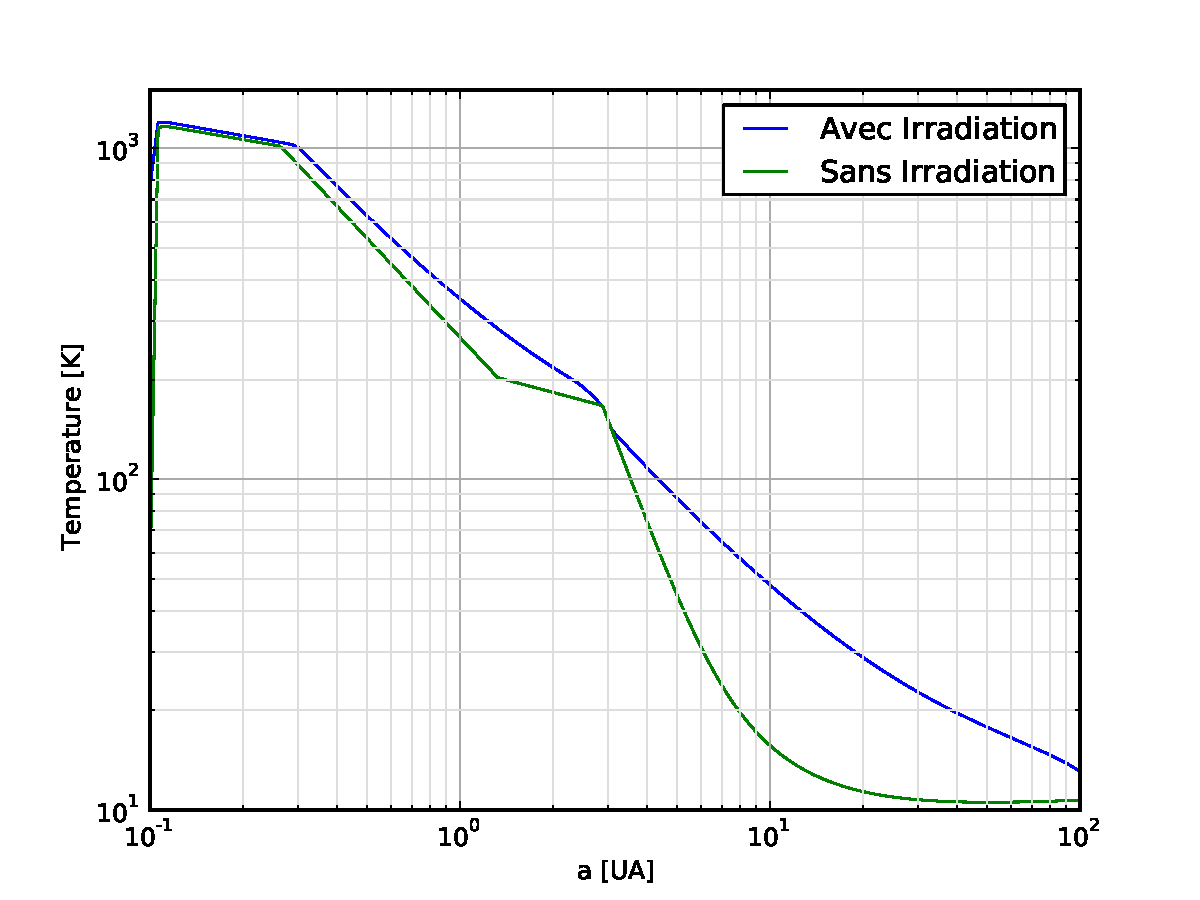
\includegraphics[width=0.6\linewidth]{figure/migration_map/temperature_with_irradiation.pdf}
\caption[Profil de température avec ou sans irradiation.]{Profil de température avec ou sans irradiation.
\refdisk}\label{fig:temp_profile_irradiation}
\end{figure}


Afin de visualiser l'effet de l'irradiation, nous avons utilisé les lois d'opacité de \cite{bell1994FU}. En effet,
le principal effet de l'irradiation est de lisser le profil de température. Sans irradiation, une discontinuité dans le régime d'opacité comme celles de \cite{bell1994FU} se répercute directement sur le profil de température \reffig{fig:temp_profile_irradiation}.
On voit donc apparaître des zones de convergence dues à des transitions d'opacité mais qui sont déformées par
l'irradiation comme on peut le constater sur \reffig{fig:irradiation}.

\begin{figure}[htbp]
\centering
\subfloat[Avec irradiation]{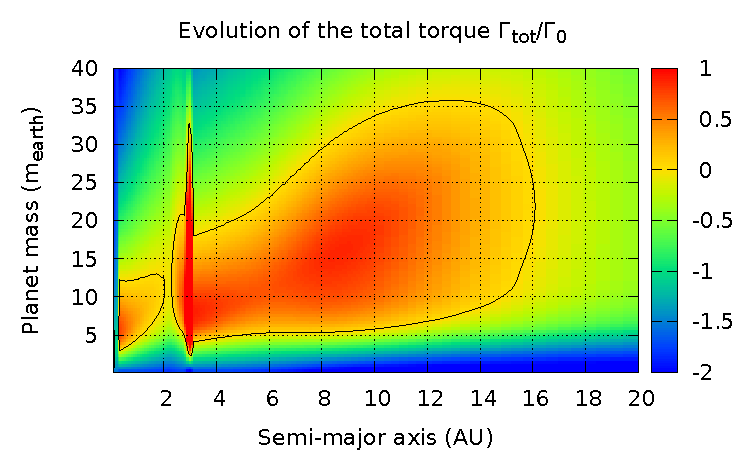
\includegraphics[width=0.49\textwidth]{figure/migration_map/bell_irr.pdf}}\hfill
\subfloat[Sans irradiation]{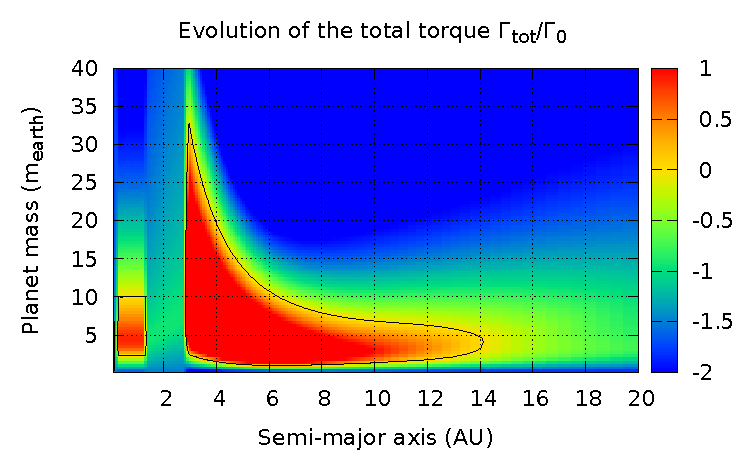
\includegraphics[width=0.49\textwidth]{%
figure/migration_map/bell_noirr.pdf}}

\caption[Carte de migration avec ou sans irradiation.]{Influence de l'irradiation sur la carte de migration à travers le profil
de température. Afin de visualiser plus
facilement les effets, l'opacité de \cite{bell1994FU} a été utilisée. \refdisk}\label{fig:irradiation}
\end{figure}

Ainsi, sans irradiation, les deux transitions d'opacité à $1.3$ et $2.9\unit{UA}$ induisent un changement brutal de la pente
du profil de température, ce qui a pour effet de changer le sens de migration (de positif à négatif, puis l'inverse).

Dans les parties externes, l'irradiation a pour effet de diminuer la pente du profil de température qui tend vers un profil en
$R^{-\sfrac37}$ quand le disque est purement passif. Dans les deux cas, la diffusion se fait essentiellement de manière radiative. La saturation du couple est sensiblement équivalente dans les cas avec et sans irradiation. La partie linéaire du couple de corotation est fortement modifiée, ainsi que la valeur du couple lui même, expliquant la modification importante de la migration dans les parties externes \reffig{fig:irradiation}.


\subsection{Effet de l'ombre du disque sur lui-même.}\label{sec:shadow}\index{self-shadowing}
Tout au long de ma thèse, j'ai considéré un modèle d'irradiation dans lequel la gestion des ombres restait sommaire. En effet, la seule ombre que je considérais était l'ombre directe. C'est-à-dire les régions du disque pour lesquelles l'échelle de hauteur décroit avec la distance. Ces zones où l'angle d'interception des rayons de l'étoile était négatif étaient détectées et l'irradiation était forcée à zéro. Nous appellerons ce modèle le \textbf{modèle direct}. C'est un modèle qui découle naturellement de la modélisation du disque. En effet, pour calculer le profil de température, on doit calculer la température point par point en partant du bord externe pour que le calcul de la température converge \citep{dullemond2000passive}. Nous n'avons donc pas accès à l'ombre réelle du disque lors du calcul de l'irradiation. L'ombre est simplement la zone où l'angle entre les rayons de l'étoile et la surface du disque est nul.

Ici, nous cherchons à comparer ce modèle avec deux modèles plus complexes où l'ombre du disque est gérée de manière plus cohérente. 

Dans ces nouveaux modèles, on calcule une première fois le profil de température du disque et on stocke la valeur de l'irradiation en chaque point du disque. Ensuite, on détecte les ombres du disque en cherchant les maxima locaux du profil d'échelle de hauteur. Pour chaque maximum local, on cherche l'ombre qu'il projette sur le disque afin d'y désactiver l'irradiation. Dans les derniers 10\% de l'étendue de l'ombre, on lisse linéairement l'irradiation en considérant que 10\% avant la fin de l'ombre, l'irradiation est égale à $0 * F_\text{irr}$ (où $F_\text{irr}$ est le chauffage d'irradiation local) et à la toute fin de l'ombre, l'irradiation vaut $1 * F_\text{irr}$. Ainsi, à la position $R_b + 0.95 * l_s$ (où $R_b$ est le rayon de la bosse du disque considérée et $l_s$ est la longueur de l'ombre qu'il projette), l'irradiation vaut la moitié de l'irradiation calculée précédemment $0.5 * F_\text{irr}$. 

J'ai testé deux cas, un cas où l'étoile est considérée ponctuelle, que nous nommerons \textbf{modèle ponctuel}, et un cas où on prend en compte le rayon de l'étoile que nous appellerons le \textbf{modèle étendu}. Dans ce dernier cas, on néglige totalement le fait qu'en sortant de l'ombre, on ne voit quasiment pas l'étoile. Dans tous les modèles, l'irradiation considère que l'étoile n'est pas ponctuelle, c'est simplement pour le calcul des ombres \emph{a posteriori} que l'on considèrera soit une étoile ponctuelle soit de rayon $R_\star$.

\reffig{fig:shadow_temp_profile} montre l'évolution du profil de température en fonction des différents modèles de l'ombre du disque. Le profil de température du \textbf{modèle direct} est simplement celui du disque de référence. L'ombre est simplement constituée des zones où l'angle de réception des rayons de l'étoile est nul. Dans ce cas, la zone d'ombre est située entre $1.46$ et $1.75\unit{UA}$.

\begin{figure}[htbp]
\centering
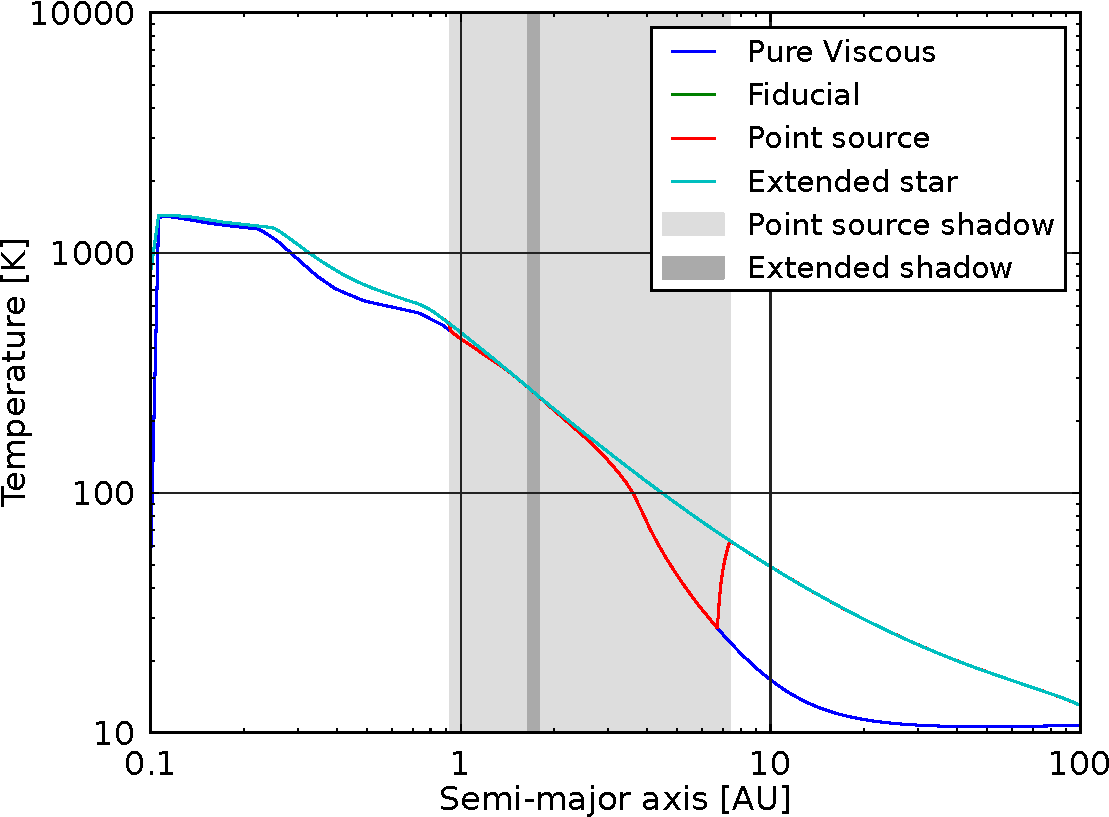
\includegraphics[width=0.49\textwidth]{figure/shadow/fiducial_temperature_profile.pdf}

\caption[Influence de l'ombre sur le profil de température]{Profils de température pour différents modèles où l'ombre du disque
sur lui-même est calculée différemment. Les profils des modèles \textbf{direct} et \textbf{étendu} sont confondus.
\refdisk}\label{fig:shadow_temp_profile}
\end{figure}

Ensuite, le \textbf{modèle ponctuel} considère l'étoile centrale comme ponctuelle, et cherche \emph{a posteriori} les ombres du disque, avant de recalculer une nouvelle fois le profil de température. Le profil de température du disque de référence dans lequel on ne tient pas compte de l'irradiation (chauffage visqueux uniquement) est représenté, afin de pouvoir comparer. Dans la zone d'ombre ainsi calculée, le profil de température est équivalent à un profil purement visqueux, sans tenir compte de l'irradiation de l'étoile. En effet, dans cette région-là, l'irradiation est forcée à 0. À noter que la température d'équilibre calculée numériquement ne tient pas compte de la diffusion de chaleur entre anneaux proches, empêchant un lissage de la transition brutale de la partie ombragée à la partie irradiée.

Maintenant, on considère que l'étoile possède un rayon $R_\star=R_\odot$ (\textbf{modèle étendu}), l'ombre qui s'étendait auparavant de $0.93$ à $7.35\unit{UA}$ dans le \textbf{modèle ponctuel} n'est plus que de $1.65$ à $1.78\unit{UA}$. L'ombre commence plus loin, car les rayons de l'étoile centrale partent de plus haut. Ils ne partent plus de $z=0$ mais de $z=0.0046\unit{UA}$. De même, la surface du disque sort beaucoup plus rapidement de l'ombre pour les mêmes raisons. En conséquence, le \textbf{modèle étendu} possède exactement le même profil que le \textbf{modèle direct}. L'ombre est dans ce cas située dans une partie totalement dominée par le chauffage visqueux et l'irradiation n'a aucune incidence sur la température du disque. 

\begin{figure}[htbp]
\centering
\subfloat[Modèle
ponctuel]{\label{fig:extended_shadow_map}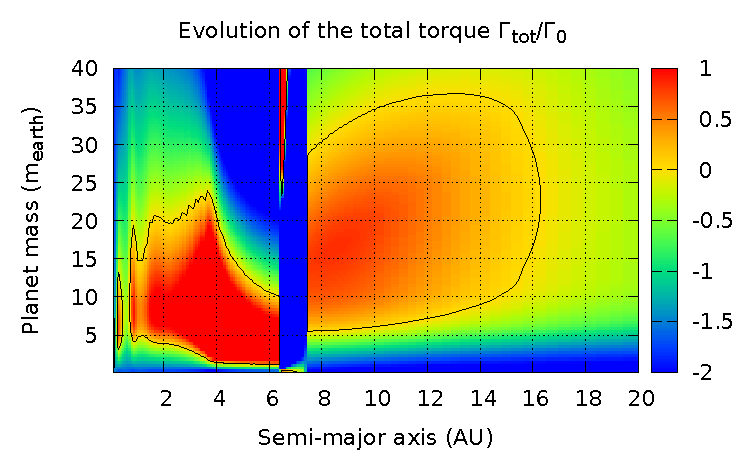
\includegraphics[width=0.49\textwidth]{figure/shadow/fiducial_shadow.pdf}}\hfill
\subfloat[Modèle étendu]{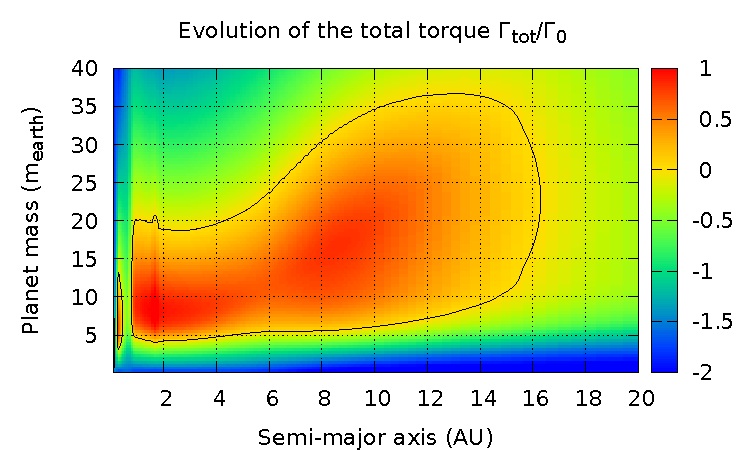
\includegraphics[width=0.49\textwidth]{%
figure/shadow/fiducial_r_star_shadow.pdf}}

\caption[Influence de l'ombre sur la carte de migration.]{Influence de la modélisation de l'ombre sur la carte de migration. 
\refdisk}\label{fig:map_shadow_effect}
\end{figure}

Les profils de températures avec les deux nouveaux modèles testés, à savoir les modèles \textbf{ponctuel} et \textbf{étendu},
nous donnent les cartes de migration \reffig{fig:map_shadow_effect}. Dans le cadre du \textbf{modèle ponctuel}, la région
d'ombre change la carte de migration. Dans l'ombre, et juste avant d'en sortir, la carte de migration est équivalente à un
disque purement actif, sans irradiation. En dehors de l'ombre, la carte de migration ne change pas. Mais à la fin de l'ombre,
près de $6\unit{UA}$, alors que le chauffage par irradiation remonte brusquement dans la région où l'ombre n'est plus
complète, une zone de transition apparait. Dans cette zone, la température monte brusquement, et le profil s'inverse. Pour les
très grandes ($m>25\mearth$) et très petites ($m<1\mearth$) masses, une zone de migration vers l'extérieur apparait, permettant
de maintenir ces planètes dans le disque, alors que les masses intermédiaires ne peuvent pas migrer vers l'extérieur dans cette
région de transition \reffig{fig:extended_shadow_map}. 

Dans le cas du \textbf{modèle étendu}, la carte de migration ne change pas par rapport au disque de référence. Dans ce modèle, l'ombre n'est pas suffisamment étendue pour atteindre les parties passives du disque, où l'irradiation est importante. Ainsi, désactiver l'irradiation ne change pas le profil de température et la migration n'est ainsi pas affectée. 

Le modèle le plus abouti pour le calcul de l'ombre est le \textbf{modèle étendu} qui recalcule l'ombre \emph{a posteriori} mais prend en compte la non-ponctualité de l'étoile. 

Pour que le calcul de l'ombre du disque ait une importance sur la carte de migration, il faut que la bosse du disque soit suffisamment importante pour qu'une partie de l'ombre soit projetée dans la partie passive du disque, là où l'irradiation est importante. \reffig{fig:shadow-example} montre un exemple d'un disque où la modélisation de l'ombre a une importance. Dans ce disque, nous avons toujours les propriétés du disque de référence, à ceci près que le profil de densité est maintenant $\Sigma(R) = 1700 * R^{-1.5}\unit{g/cm^2}$. 

\begin{figure}[htbp]
\centering
\subfloat[Modèle direct]{\label{fig:label1}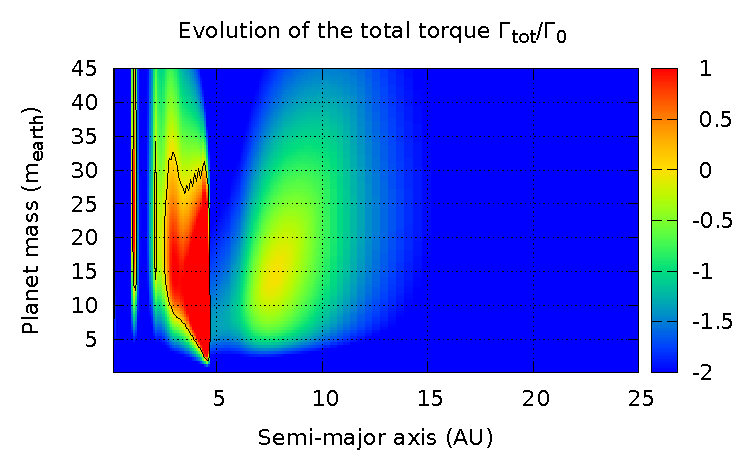
\includegraphics[width=0.49\textwidth]{figure/shadow/example_with_direct_shadow.pdf}}\hfill
\subfloat[Modèle étendu]{\label{fig:label2}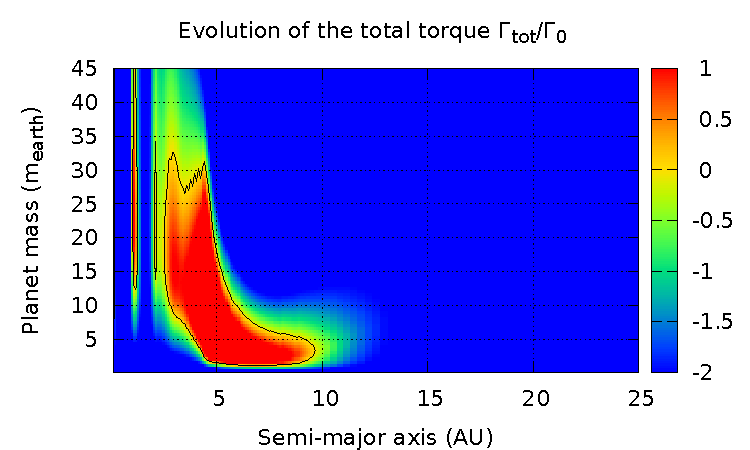
\includegraphics[width=0.49\textwidth]{figure/shadow/example_with_shadow.pdf}}
\caption[Influence de l'ombre sur la carte de migration d'un disque massif.]{Effet des modèles pour l'ombre du disque sur la
carte de migration dans un cas où la densité de surface vaut $\Sigma(R) = 1700 * R^{-1.5}\unit{g/cm^2}$.
\refdisk}\label{fig:shadow-example}
\end{figure}

Dans ce cas, la température extrêmement élevée au bord interne cause l'apparition d'une bosse très importante au bord interne du disque qui masque totalement l'étoile dans le cas où le calcul de l'ombre du disque se fait \emph{a posteriori}. Les deux profils de température et les ombres correspondantes sont représentés \reffig{fig:example_shadow_temp_profile}. 

\begin{figure}[htbp]
\centering
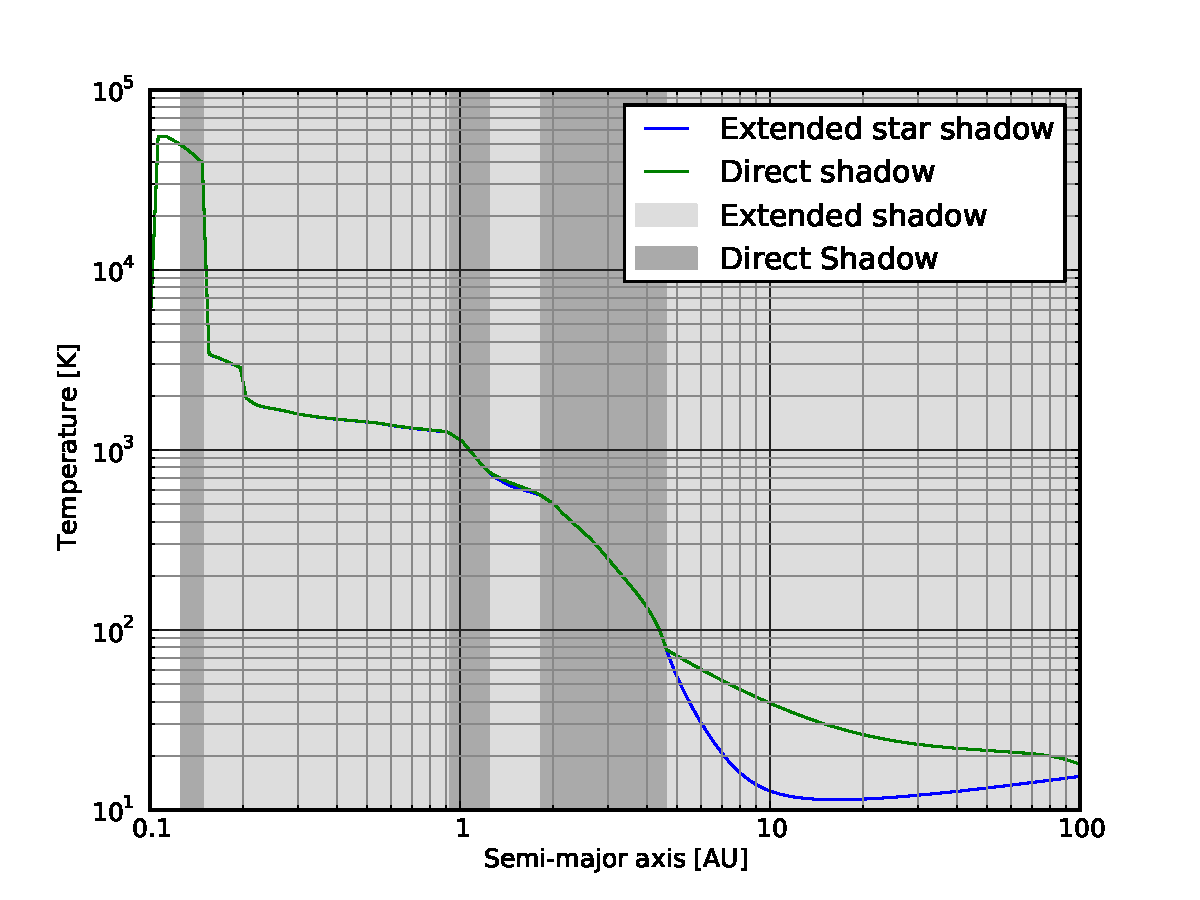
\includegraphics[width=0.65\linewidth]{figure/shadow/example_shadow_temp_profile.pdf}
\caption[Influence de l'ombre sur le profil de température d'un disque massif.]{Profil de température et ombre du disque dans le
cas du modèle direct ou étendu pour la modélisation de l'ombre. La densité de surface vaut $\Sigma(R) = 1700 *
R^{-1.5}\unit{g/cm^2}$. \refdisk}\label{fig:example_shadow_temp_profile}
\end{figure}

Malgré tout, le \textbf{modèle étendu} ne prend pas en compte le fait qu'au delà de cette zone d'ombre, il y a toute une zone où l'irradiation de l'étoile est partielle, dû au fait qu'une partie de l'étoile est masquée par le disque. Il ne prend pas non plus en compte l'auto-irradiation, c'est-à-dire le fait que des parties du disque peuvent en illuminer d'autres, compte tenu du fait qu'on a le profil d'échelle de hauteur qui se creuse à cet endroit-là. Cet effet sera d'autant plus marqué que la température du disque est importante et que la bosse du disque est grande. 

De plus, les cas où ce nouveau modèle pour l'ombre du disque a un effet important sont des cas limites. En effet, dans l'exemple présenté ici \reffig{fig:shadow-example}, la température au bord interne dépasse $50 000\unit{K}$. Dans des disques beaucoup plus classiques, avec des températures inférieures à $10 000\unit{K}$ au bord interne, nous avons vu que le modèle classique pour l'ombre du disque marchait bien, car l'ombre se trouvait dans la partie active du disque, là où l'irradiation joue un rôle mineur sur le profil de température.

\subsection{Effet des propriétés de l'étoile}
Pour le modèle de référence, les propriétés de l'étoile sont celles du Soleil, même rayon même température. Mais les propriétés des étoiles au moment de la formation planétaire ne sont pas celles d'une étoile évoluée comme le Soleil. Elles ont tendance à être moins chaudes, et plus grosses que le Soleil. À partir de \cite[Table 2]{hartigan1995disk}, \reffig{fig:TTauri_sample} représente 42 étoiles T Tauri dans un diagramme avec leur rayon en abscisse et leur température en ordonnée. 

\begin{figure}[htbp]
\centering
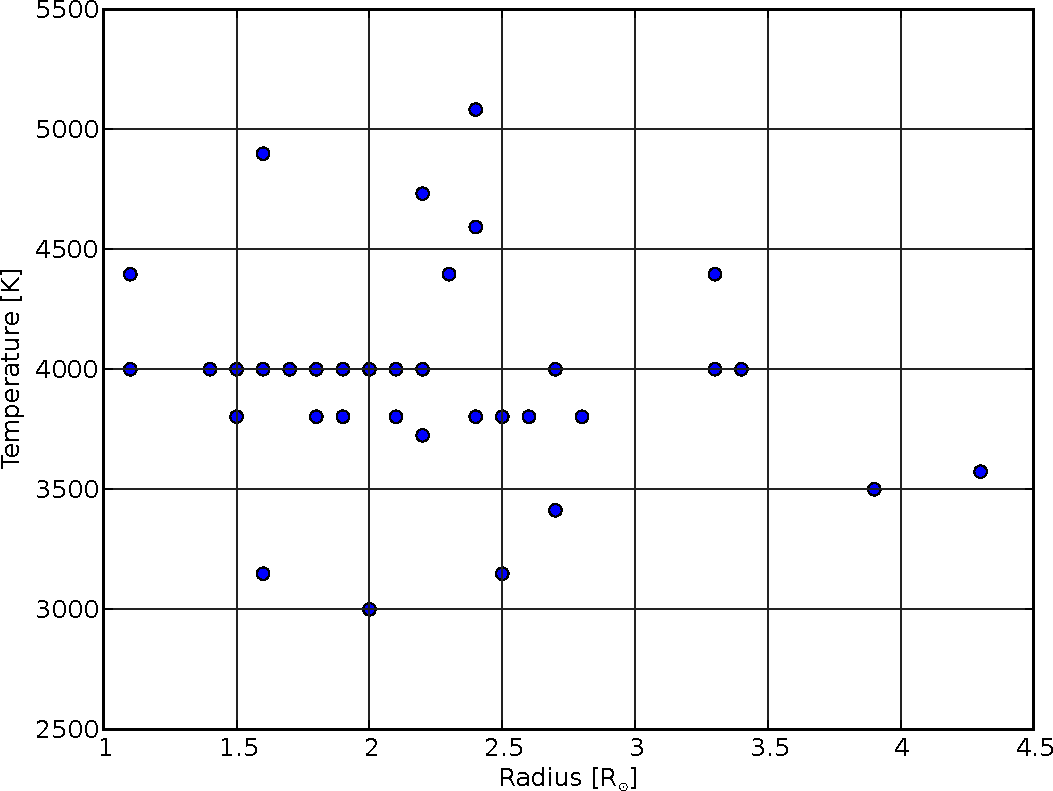
\includegraphics[width=0.5\linewidth]{figure/TTauri_sample.pdf}
\caption[Propriétés d'un échantillon d'étoiles T Tauri détectées.]{Représentation d'un échantillon d'étoiles T Tauri
\citep{hartigan1995disk}. }\label{fig:TTauri_sample}
\end{figure}

Nous souhaitons voir l'influence des propriétés de l'étoile vis-à-vis de l'irradiation. Nous allons maintenant faire varier le rayon $R_\star$ et la température $T_\star$ de l'étoile au centre du disque. 

\begin{figure}[htbp]
\centering
\subfloat[$R_\star=1.5\unit{R_\odot}$ ; $T=4000\unit{K}$]{\label{fig:low_TTauri}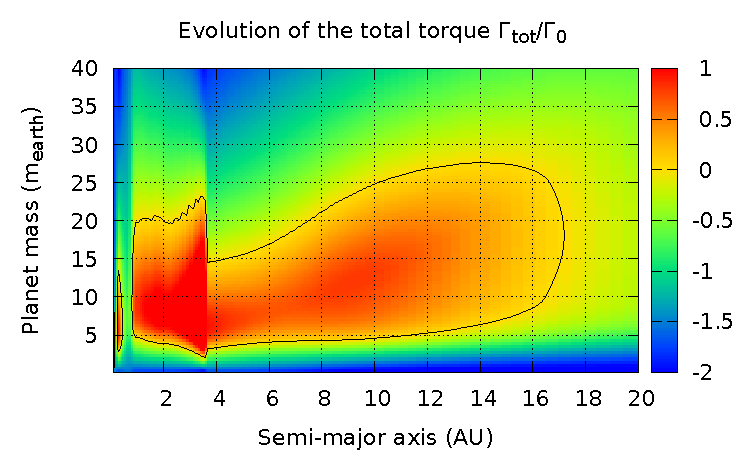
\includegraphics[width=0.49\textwidth]{figure/migration_map/TTauri/R_15_T_4000.pdf}}
\hfill
\subfloat[$R_\star=2.5\unit{R_\odot}$ ; $T=3500\unit{K}$]{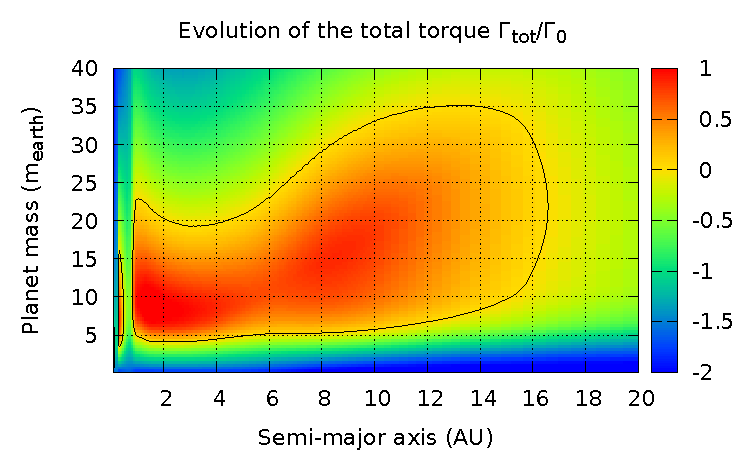
\includegraphics[width=0.49\textwidth]{%
figure/migration_map/TTauri/R_25_T_3500.pdf}}

\subfloat[$R_\star=2.5\unit{R_\odot}$ ; $T=4000\unit{K}$]{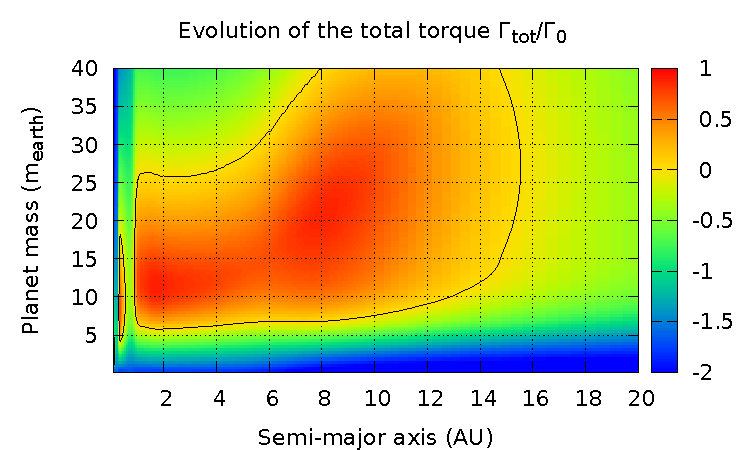
\includegraphics[width=0.49\textwidth]{figure/migration_map/TTauri/R_25_T_4000.pdf}}\hfill
\subfloat[$R_\star=2.5\unit{R_\odot}$ ; $T=4500\unit{K}$]{\label{fig:high_TTauri}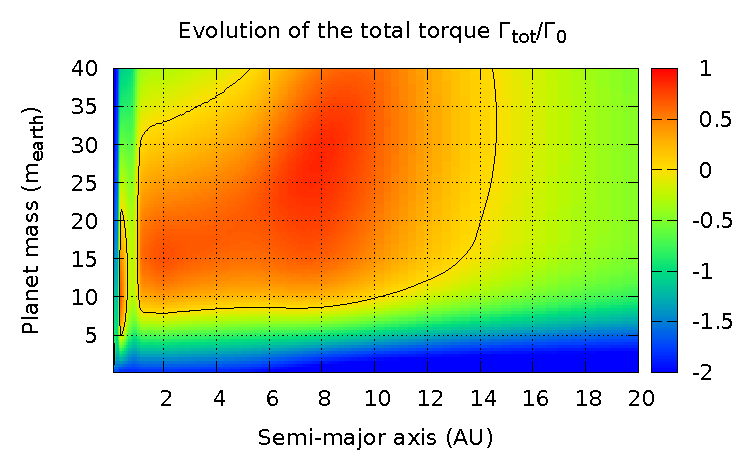
\includegraphics[width=0.49\textwidth]{figure/migration_map/TTauri/R_25_T_4500.pdf}}
\caption[Influence des propriétés de l'étoile centrale sur la carte de migration.]{Influence du rayon $R_\star$ et de la
température $T_\star$ de l'étoile centrale sur la carte de migration au travers de l'irradiation. Les luminosités
correspondantes pour les cartes (a), (b), (c) et (d) sont respectivement $0.5\unit{L_\odot}$, $0.84\unit{L_\odot}$,
$1.43\unit{L_\odot}$ et $2.30\unit{L_\odot}$. \refdisk}\label{fig:map_TTauri}
\end{figure}

À partir des 4 étoiles T Tauri typiques que nous avons choisies, nous avons l'effet de la luminosité de l'étoile sur la carte de migration. En effet, il y a une dégénérescence entre le rayon et la température de l'étoile, si on considère une étoile ponctuelle. Les cartes ont été classées de la plus faible à la plus grande luminosité, les luminosités allant de $0.5\unit{L_\odot}$ à $2.30\unit{L_\odot}$. À mesure que l'irradiation de l'étoile augmente, le profil de température augmente au travers du disque de manière quasi-uniforme. L'irradiation joue ici sur les masses critiques minimales et maximales au delà desquelles la migration vers l'intérieur est systématique. En particulier, les planètes de $4\mearth$ peuvent migrer vers l'extérieur dans le premier disque \reffig{fig:low_TTauri}, alors qu'il faut qu'elle aient au minimum $8\mearth$ pour pouvoir migrer dans le dernier disque \reffig{fig:high_TTauri} où l'irradiation est la plus forte. 

\bigskip

Nous avons vu dans la partie précédente l'effet de l'ombre du disque. Nous souhaitons maintenant voir ce qu'il en est quand, à
luminosité constante, on varie le rayon et la température de l'étoile \reffig{fig:map_TTauri_radius}. À mesure que le rayon de
l'étoile augmente, les ombres du disque s'amenuisent car les parties supérieures de la sphère stellaire deviennent visibles.
Ainsi, on remarque que la bosse sur la carte de migration disparait à mesure que le rayon de l'étoile augmente. 

\begin{figure}[htbp]
\centering
\subfloat[$R_\star=0.5\unit{R_\odot}$ ; $T=8061\unit{K}$]{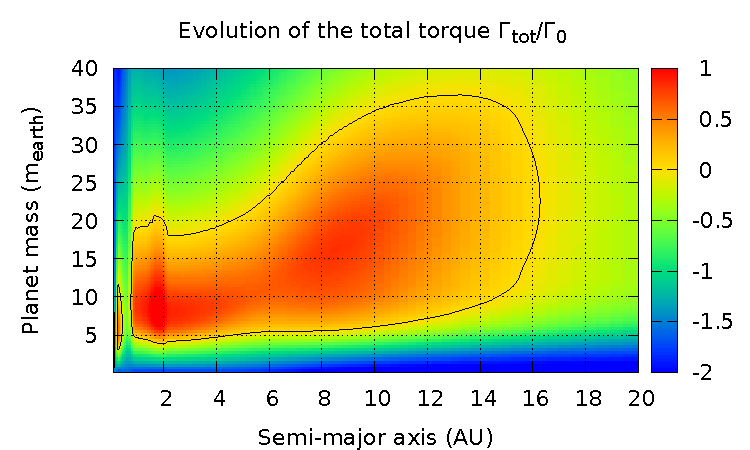
\includegraphics[width=0.49\textwidth]{figure/migration_map/TTauri/R_05_T_8061.pdf}}
\hfill
\subfloat[$R_\star=\unit{R_\odot}$ ; $T=5700\unit{K}$]{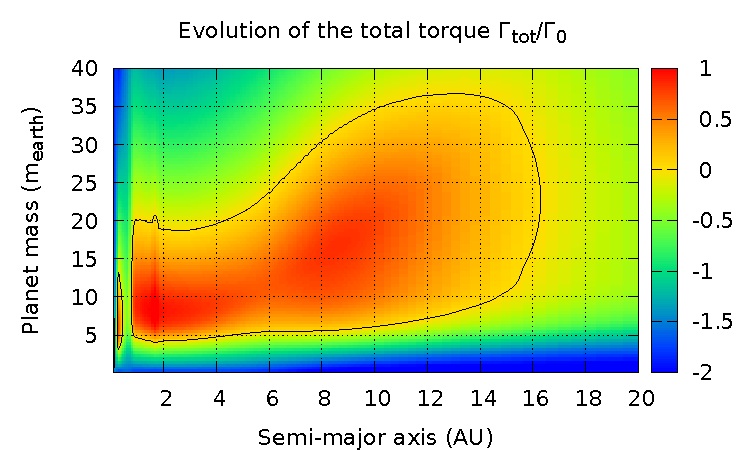
\includegraphics[width=0.49\textwidth]{%
figure/migration_map/TTauri/R_10_T_5700.pdf}}

\subfloat[$R_\star=2\unit{R_\odot}$ ; $T=4031\unit{K}$]{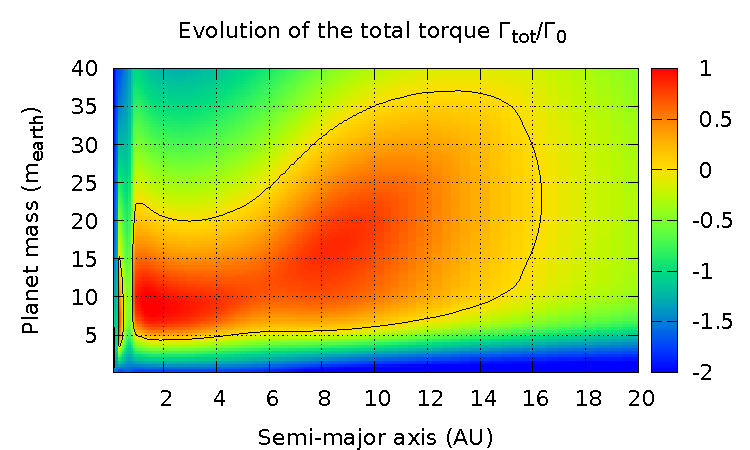
\includegraphics[width=0.49\textwidth]{figure/migration_map/TTauri/R_20_T_4031.pdf}}\hfill
\subfloat[$R_\star=4\unit{R_\odot}$ ; $T=2850\unit{K}$]{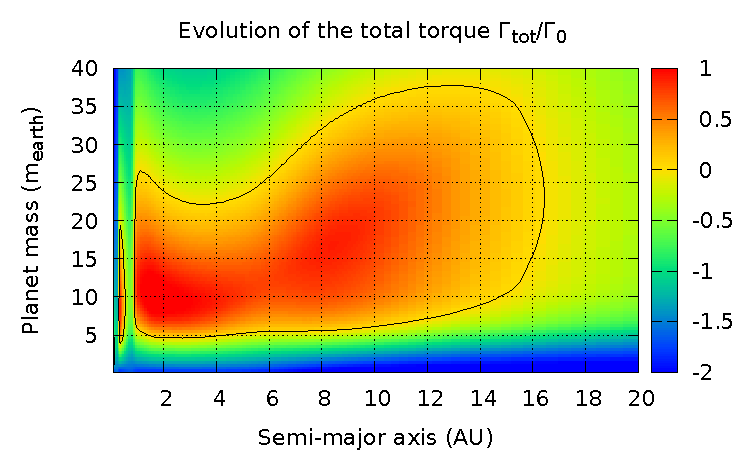
\includegraphics[width=0.49\textwidth]{figure/migration_map/TTauri/R_40_T_2850.pdf}}
\caption[Influence du rayon stellaire sur la carte de migration à flux stellaire constant.]{Influence du rayon $R_\star$ de
l'étoile centrale sur la carte de migration tandis que la luminosité de l'étoile est
conservée en variant la température. \refdisk}\label{fig:map_TTauri_radius}
\end{figure}

Le rayon plus grand $R\sim 2.5R_\odot$ des T Tauri par rapport à des étoiles plus âgées \reffig{fig:TTauri_sample} tend à atténuer les régions ombrées (\og self-shadowing\fg) du disque. Au cours de son évolution, une étoile T Tauri se contracte. À mesure que son rayon diminue, des ombres pourraient donc apparaître dans le disque, modifiant brutalement la carte de migration qui évoluait via la dissipation du disque.

\section{Influence de la viscosité du disque}
\subsection{Viscosité constante}\label{sec:nu_constant}

\begin{figure}[htbp]
\centering
\subfloat[$\nu=10^{14}\unit{cm^2/s}$]{\label{fig:nu_1e14}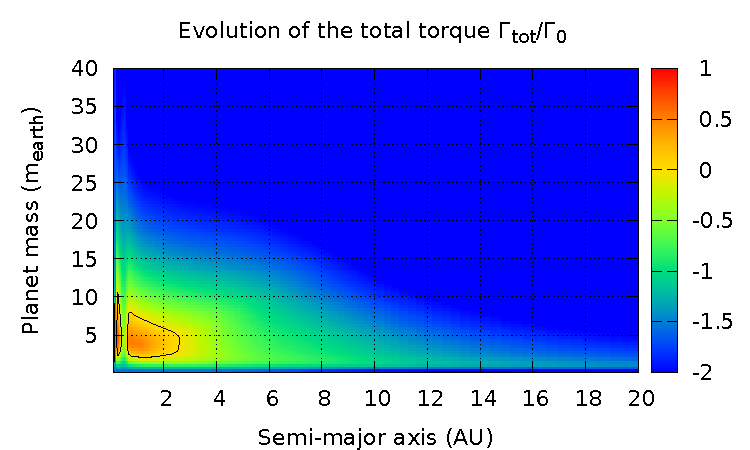
\includegraphics[width=0.49\textwidth]{figure/migration_map/viscosity/constant_1e14.pdf}}
\hfill
\subfloat[$\nu=5\cdot 10^{14}\unit{cm^2/s}$]{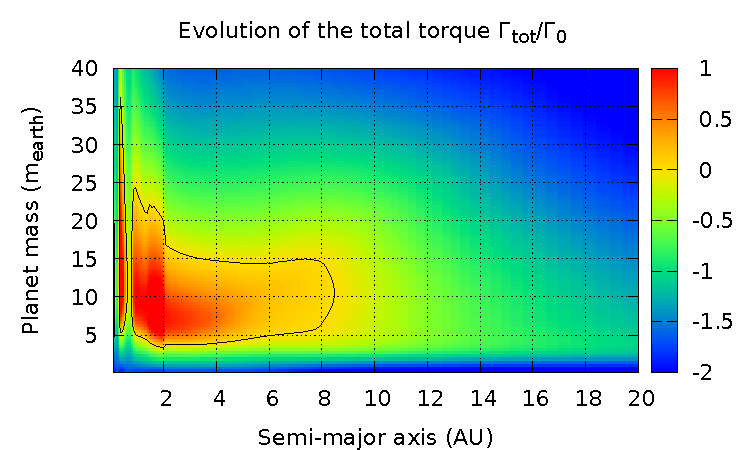
\includegraphics[width=0.49\textwidth]{figure/migration_map/viscosity/constant_5e14.pdf}}


\subfloat[$\nu=10^{15}\unit{cm^2/s}$]{\label{fig:nu_1e15}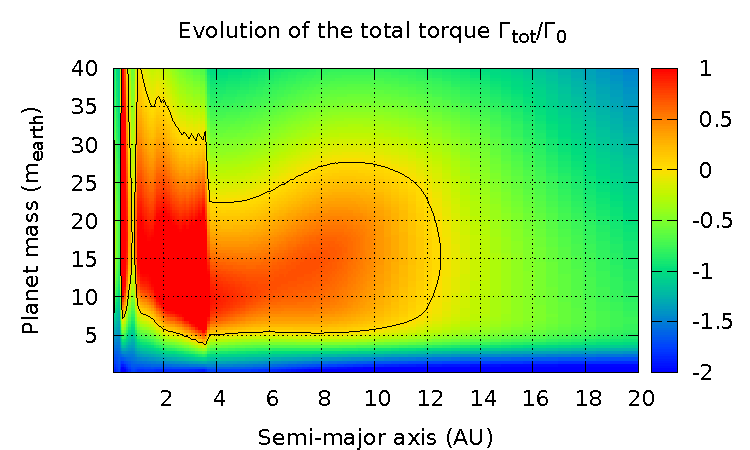
\includegraphics[width=0.49\textwidth]{%
figure/migration_map/viscosity/constant_1e15.pdf}}\hfill
\subfloat[$\nu=5\cdot 10^{15}\unit{cm^2/s}$]{\label{fig:nu_5e15}\includegraphics[width=0.49\textwidth]{figure/migration_map/viscosity/constant_5e15.pdf}}
\caption[Influence de la viscosité sur la carte de migration.]{Influence de la viscosité sur la carte de migration.
\refdisk}\label{fig:constant_viscosity}
\end{figure}

Le couple de migration est sensible à la valeur de la viscosité $\nu$ \reffig{fig:constant_viscosity}. À mesure que la
viscosité augmente, le chauffage visqueux en fait autant. La température augmente de manière générale dans le disque. Les
zones de migration vers l'extérieur se dilatent en même temps qu'elles se déplacent dans les parties externes du disque. Les
transitions d'opacité se déplacent également vers l'extérieur. 

De plus la viscosité agit sur la saturation du couple de corotation.
Quand la viscosité augmente, le temps de diffusion visqueuse $t_\text{visc}$ diminue. Le couple de corotation ne sature pas tant
que $(t_\text{visc} < t_\text{lib}/2)$. Si on augmente la viscosité $\nu$, le couple de corotation sature moins facilement à
mesure que la masse de la planète augmente. La partie supérieure de la carte de migration se décale vers le haut quand la
viscosité augmente. 

Mais l'augmentation de la viscosité a un effet indirect sur le temps de diffusion radiative $t_\text{rad}$. Si la viscosité augmente, le chauffage visqueux augmente. La température augmente, et la diffusivité thermique $\chi$ avec. Ainsi, quand la viscosité augmente, le temps de diffusion radiative $t_\text{rad}$ diminue. Le couple de corotation est linéaire quand $t_\text{rad} < t_\text{U-turn}$. Quand la viscosité $\nu$ augmente, le couple de corotation se linéarise plus rapidement à mesure que la masse de la planète diminue. La partie inférieure de la carte de migration se décale elle aussi vers le haut. Des planètes de faible masse qui migraient vers l'extérieur ne peuvent plus migrer que vers l'intérieur à mesure que la viscosité augmente. 

\subsection{Viscosité alpha}\index{prescription alpha}
La prescription alpha \citep{shakura1973black} est une autre manière de définir la viscosité, à partir d'un paramètre adimensionné $\alpha$ \refsec{sec:viscosite-alpha}.

\begin{figure}[htbp]
\centering
\includegraphics[width=0.6\linewidth]{figure/migration_map/viscosity/alpha_profiles.pdf}
\caption[Profils de viscosité dans le disque pour différentes valeurs d'alpha.]{Profils de viscosité du disque en fonction de
la valeur d'alpha. Ces profils correspondent à chacune des quatre cartes de migration
présentées \protect\reffig{fig:alpha_viscosity}. \refdisk}\label{fig:alpha_profiles}
\end{figure}

Par rapport à un modèle où la viscosité est constante, la prescription alpha entraine une augmentation continue de la viscosité
en fonction de la distance \reffig{fig:alpha_profiles}. Pourtant, ce n'est pas un simple facteur multiplicateur de la viscosité
en raison du fait qu'il y a maintenant une dépendance en température au travers de l'échelle de hauteur et la vitesse du son.
Les variations de $\alpha$ peuvent ainsi faire apparaître des transitions d'opacité au sein même du profil de viscosité. 

\begin{figure}[htbp]
\centering
\subfloat[$\alpha=10^{-2}$]{\includegraphics[width=0.49\textwidth]{figure/migration_map/viscosity/alpha_1e-2.pdf}}
\hfill
\subfloat[$\alpha=5\cdot 10^{-3}$]{\label{fig:alpha_5e-3}\includegraphics[width=0.49\textwidth]{figure/migration_map/viscosity/alpha_5e-3.pdf}}

\subfloat[$\alpha=10^{-3}$]{\label{fig:alpha_1e-3}\includegraphics[width=0.49\textwidth]{%
figure/migration_map/viscosity/alpha_1e-3.pdf}}\hfill
\subfloat[$\alpha=5\cdot
10^{-4}$]{\label{fig:alpha_5e-4}\includegraphics[width=0.49\textwidth]{figure/migration_map/viscosity/alpha_5e-4.pdf}}
\caption[Influence d'alpha sur la carte de migration.]{Influence de la valeur de $\alpha$ dans le cadre d'une prescription
alpha pour la viscosité. \refdisk}\label{fig:alpha_viscosity}
\end{figure}

On fait varier la valeur de $\alpha$ dans une plage de valeurs tirée des observations \citep{guilloteau2011dual}. Dans les
disques jeunes, $\alpha$ peut atteindre $10^{-2}$, tandis que les disques un peu plus âgés \cite[fig.
16]{guilloteau2011dual} montrent des valeurs plus basses. Nous prenons comme plage de valeurs à étudier $\alpha\in[5\cdot
10^{-4} ; 10^{-2}]$. 

Pour une valeur d'alpha donnée, la viscosité varie à travers le disque. Si on prend l'exemple de $\nu=10^{14}\unit{cm^2/s}$ \reffig{fig:nu_1e14}, cette viscosité est atteinte à $0.2\unit{UA}$ pour notre disque de référence avec $\alpha=5\cdot 10^{-3}$. La carte de migration dans cette région, autour de $0.2\unit{UA}$ est similaire dans le cas de la viscosité constante ou du modèle alpha. On remarque la même chose si on s'intéresse maintenant à $\nu=10^{15}\unit{cm^2/s}$ \reffig{fig:nu_1e15}, ce qui correspond à la zone autour de $6\unit{UA}$ pour notre disque de référence \reffig{fig:alpha_5e-3}.

Par contre, si nous cherchons à comparer $\nu=5\cdot 10^{15}\unit{cm^2/s}$ \reffig{fig:nu_5e15} avec le modèle $\alpha=5\cdot 10^{-3}$ \reffig{fig:alpha_5e-3} nous ne constatons aucune zone où la carte de migration est similaire. Le fait est que cela correspond à la zone autour de $45\unit{UA}$, région dans laquelle l'irradiation domine. Nous voyons donc qu'à viscosité équivalente, nous ne pouvons comparer un modèle alpha avec un modèle à viscosité constante uniquement dans les régions actives du disque, là où le chauffage visqueux domine. En effet, dans ces régions-là, la viscosité étant l'origine principale de la température, c'est elle qui gouverne la carte de migration. 

Enfin, les cartes où $\alpha$ est très faible \reffig{fig:alpha_1e-3} et \reffig{fig:alpha_5e-4} montrent qu'à mesure qu'alpha
diminue, la viscosité fait de même de manière globale dans le disque. Dans ces disques-là, on constate la disparition
progressive de la totalité des zones de convergence. Ainsi, dans le disque où alpha est le plus faible ($\alpha=5\cdot 10^{-4}$),
toutes les planètes migrent vers l'intérieur \reffig{fig:alpha_5e-4}, quelle que soit leur masse ou leur position dans le
disque.

\subsection{Zone morte}\index{zone morte}
\begin{figure}[htbp]
\centering
\includegraphics[width=0.6\linewidth]{figure/migration_map/viscosity/dead_zone_profile.pdf}
\caption[Effet d'une zone morte sur la viscosité.]{Profils de viscosité du disque selon qu'une zone morte est modélisée ou pas.
En dehors de la zone morte $\alpha=5\cdot 10^{-3}$. Dans la zone morte, $\alpha=10^{-4}$. Ces profils correspondent à chacune
des deux cartes de migration
présentées \protect\reffig{fig:viscosity_DZ}. \refdisk}\label{fig:dead_zone_profile}
\end{figure}

Une zone morte, ou \og dead zone\fg est une région d'un disque protoplanétaire où la turbulence est faible en raison d'un taux
d'ionisation extrêmement bas empêchant tout couplage du gaz du disque avec le champ magnétique de l'étoile
\refsec{sec:ionisation_DZ}.

Dans la zone morte, la viscosité chute rapidement, et augmente en fonction de la distance dans un régime différent que dans le reste du disque \reffig{fig:dead_zone_profile}. 

\begin{figure}[htbp]
\centering
\subfloat[Sans zone morte]{\includegraphics[width=0.49\textwidth]{figure/migration_map/viscosity/alpha_5e-3.pdf}}\hfill
\subfloat[Avec zone morte]{\includegraphics[width=0.49\textwidth]{%
figure/migration_map/viscosity/alpha_dz.pdf}}

\caption[Effet d'une zone morte sur la carte de migration.]{Effet d'une zone morte sur la carte de migration. Au cœur de la dead
zone, $\alpha=10^{-4}$. En dehors, $\alpha=5\cdot 10^{-3}$. Dans les zones de transition, la valeur de $\alpha$ est lissée. La
zone morte s'étend de $1$ à $10\unit{UA}$. Plus de détails sur la modélisation de la zone morte \protect\refsec{sec:dead_zone}.
\refdisk}\label{fig:viscosity_DZ}
\end{figure}

Sur les cartes de migration \reffig{fig:viscosity_DZ}, l'entrée dans la zone morte modifie en profondeur la carte de migration en creusant une zone de migration vers l'intérieur en raison de la viscosité très faible. Le temps de diffusion visqueuse $t_\text{visc}$ augmente alors brusquement, engendrant la saturation rapide du couple de corotation quelle que soit la masse de la planète. Ainsi, dans la zone morte, la possibilité de migration vers l'extérieur est fortement réduite. En dehors de la zone morte, la carte de migration est quasi inchangée.

\bigskip

Maintenant, on cherche à voir l'effet conjoint d'une zone morte et de l'ombre du disque modélisée de manière complexe (\textbf{modèle étendu}) dans \refsec{sec:shadow}.

Au bord interne de la zone morte, où le chauffage visqueux domine, la brusque diminution de la viscosité entraine une diminution de la température, l'irradiation de l'étoile devient temporairement dominante par rapport au chauffage visqueux. Comme nous l'avions vu en fin de \refsec{sec:shadow} l'effet de l'ombre ne devient important que dans les parties passives du disque, ce qu'est le bord interne de la zone morte à cause de la brusque diminution de la viscosité. Ainsi, au bord interne de la zone morte, l'ombre du disque joue un rôle important \reffig{fig:dz_shadow_temp}. Elle fait apparaître une zone de convergence pour les planètes de faibles masses qui autrement migrent vers l'intérieur \reffig{fig:dz_shadow_map}.

\begin{figure}[htbp]
\centering
\subfloat[Carte de migration]{\label{fig:dz_shadow_map}\includegraphics[width=0.49\textwidth]{figure/migration_map/viscosity/dz_shadow.pdf}}\hfill
\subfloat[Profil de température]{\label{fig:dz_shadow_temp}\includegraphics[width=0.49\textwidth]{%
figure/migration_map/viscosity/dz_shadow_temp_profile.pdf}}

\caption[Effets conjoint d'une zone morte et du self-shadowing sur la carte de migration.]{Effet conjoint d'une zone morte et du
\og self-shadowing\fg. La zone morte s'étend de $1$ à $10\unit{UA}$. Plus de détails sur la modélisation de la zone morte
\protect\refsec{sec:dead_zone}. \refdisk}\label{fig:dz_shadow}
\end{figure}

Cette soudaine chute de la température entraine une augmentation du temps de diffusion radiative $t_\text{rad}$. Cette
augmentation du temps de diffusion rend beaucoup plus difficile pour le couple de corotation de tendre vers sa valeur linéaire.
Même pour des planètes de faible masse, le couple de corotation est non-linéaire et fait apparaître une zone de migration
vers l'extérieur au début de la zone morte, peu après $1\unit{UA}$. 

Cette zone de convergence sera sans doute très intéressante au niveau de l'accrétion de masse et de la formation des
planètes car peu étendue, mais elle pourrait malgré tout jouer un rôle majeur en maintenant des planètes telluriques de faibles
masses (de l'ordre de $1\mearth$) dans le disque, sans besoin d'aucuns compagnons massifs en résonance pour la maintenir.

La modélisation poussée de l'ombre du disque et son effet sur l'irradiation pourraient donc jouer un rôle majeur au niveau des
zones mortes où une zone locale où l'irradiation domine apparaît à cause de la décroissance soudaine de la viscosité et du chauffage
qui en découle \citep{matsumura2003origin}.

Malgré tout, il est important de noter que la modélisation de la zone morte est ici très artificielle. Il n'y a pas de couplage entre viscosité et densité de surface. Dans un disque où le taux d'accrétion est constant $\dot{M}=\cte$, une baisse de viscosité entraine une augmentation de la densité. Le chauffage visqueux est donc le même dans la zone morte et à l'extérieur de celle-ci.

\section{Profil de densité de surface}
Dans notre modèle, le profil de la densité de surface est notre plus grande incertitude. Les contraintes observationnelles ne
restreignent pas suffisamment le profil de densité \citep[Fig. 12]{mundy2000structure, andrews2007high, williams2011protoplanetary,
guilloteau2011dual}. C'est à partir de ce profil de densité de surface que nous calculons toutes les propriétés du disque, en
particulier la température et l'échelle de hauteur, puis la migration des planètes. 

On définit la loi de puissance pour la densité de surface de la façon suivante : 
\begin{align}
\Sigma(R) &= \Sigma_0 * \left(\frac{R}{R_0}\right)^{-d}
\end{align}
où $\Sigma_0$ est la densité de surface à $R_0=1\unit{UA}$.

À l'instar de
la viscosité $\nu$, le profil de densité de surface $\Sigma$ influence directement le chauffage visqueux. Cependant, changer la
densité de surface permet de modifier le chauffage visqueux sans modifier le temps de diffusion visqueuse $t_\nu$. Je cherche à
étudier l'influence de l'indice $d$ de la loi de puissance sur la carte de migration, soit en le faisant varier
individuellement, soit en regardant, à masse du disque constante, ce que le profil de densité change. 

\subsection{Variation de l'indice d}\label{sec:sigma_index}
\begin{figure}[htbp]
\centering
\subfloat[$d=0.6$]{\label{fig:d06}\includegraphics[width=0.49\textwidth]{%
figure/migration_map/index/sigma/300_06.pdf}}\hfill
\subfloat[$d=0.7$]{\label{fig:d07}\includegraphics[width=0.49\textwidth]{figure/migration_map/index/sigma/300_07.pdf}}

\subfloat[$d=1$]{\includegraphics[width=0.49\textwidth]{%
figure/migration_map/index/sigma/300_10.pdf}}\hfill
\subfloat[$d=1.5$]{\includegraphics[width=0.49\textwidth]{figure/migration_map/index/sigma/300_15.pdf}}

\caption[Influence du profil de densité sur la carte de migration.]{Influence de l'indice $d$ de la loi de puissance définissant
la densité de surface du disque sur la carte de migration.
Ici, $\Sigma_0=\cte=300\unit{g/cm^2}$, seul l'indice $d$ du profil de densité de surface varie. \refdisk}\label{fig:map_index}
\end{figure}

Si l'indice $d$ du profil de densité de surface augmente, la forme de la carte de migration aura tendance à se compresser autour
du rayon $R_0=1\unit{UA}$ où est définie la densité $\Sigma_0$ \reffig{fig:map_index}. En effet, pour $\Sigma_0$ fixé, si on
augmente $d$, alors on augmente la masse du disque en dessous de $R_0$ tandis qu'on diminue sa masse au delà de $\Sigma_0$
\reffig{fig:index_density}. Cette modification de la masse joue sur le chauffage visqueux et donc sur le profil de température
qui décroit plus rapidement en fonction du rayon \reffig{fig:index_temp}. En dessous de $R_0$, la température est plus
importante à mesure que $d$ augmente. Au delà de $R_0$ c'est l'inverse. Dans les parties externes où le chauffage visqueux ne
joue aucun rôle, c'est l'irradiation qui détermine la température. La densité joue encore un rôle au travers de l'opacité dans
la partie passive du disque, jusqu'à ce que l'opacité ne dépende quasiment plus de la densité (à température faible
$T<100\unit{K}$).

\begin{figure}[htbp]
\centering
\subfloat[Profils de densité]{\label{fig:index_density}\includegraphics[width=0.49\textwidth]{%
figure/migration_map/index/sigma/density_profile.pdf}}\hfill
\subfloat[Profils de
température]{\label{fig:index_temp}\includegraphics[width=0.49\textwidth]{%
figure/migration_map/index/sigma/temperature_profile.pdf}}

\caption{Profils de densité et température pour les 4 cartes de migration présentées
\protect\reffig{fig:map_index}.}\label{fig:index_profiles}
\end{figure}

\subsection{Dissipation du disque}\label{sec:sigma_0}\index{dissipation du disque}

\begin{figure}[htbp]
\centering
\subfloat[$\Sigma_0=1200\unit{g/cm^2}$]{\label{fig:1200_map}\includegraphics[width=0.49\textwidth]{%
figure/migration_map/total_mass/1200_05.pdf}}\hfill
\subfloat[$\Sigma_0=600\unit{g/cm^2}$]{\label{fig:600_map}\includegraphics[width=0.49\textwidth]{%
figure/migration_map/total_mass/600_05.pdf}}

\subfloat[$\Sigma_0=300\unit{g/cm^2}$]{\includegraphics[width=0.49\textwidth]{%
figure/migration_map/total_mass/300_05.pdf}}\hfill
\subfloat[$\Sigma_0=150\unit{g/cm^2}$]{\includegraphics[width=0.49\textwidth]{%
figure/migration_map/total_mass/150_05.pdf}}

\caption[Effet de la dissipation sur la carte de migration.]{Par rapport au disque de référence, possédant un profil de densité
de surface $\Sigma(R) = 300 \cdot
R^{-\sfrac{1}{2}}\unit{g/cm^2}$ nous représentons les cartes de migration pour des disques où nous avons changé la masse. D'en haut à gauche vers en bas à droite, ces cartes représentent les premiers stades de la dissipation du disque. \refdisk}\label{fig:map_total_mass}
\end{figure}

Étudier l'influence de la masse du disque nous permet de remonter à l'effet de la dissipation du disque. En particulier dans la
première phase de la dissipation, quand le profil de densité de surface n'évolue pas beaucoup. Dans la seconde partie gouvernée
par la photo-évaporation, la dissipation ne conserve pas le profil en loi de puissance de la densité de surface (en faisant
l'approximation que ce dernier en est un initialement) \reffig{fig:disk_dispersion}. Au lieu de ça, le
disque va se creuser à partir d'un certain rayon, optimal vis-à-vis de la photo-évaporation. Le disque va alors se scinder en
deux, la partie interne va rapidement tomber sur l'étoile centrale et dans un dernier stade les parties externes vont aussi se
dissiper. Si les détails de la dissipation ne sont pas connus, il apparait malgré tout qu'une unique décroissance exponentielle
du disque tout au long de sa vie ne représente pas fidèlement l'évolution du disque \citep{alexander2006photoevaporation}. Dans
le cadre de la migration planétaire où les profils de densité et de température jouent un rôle fondamental, nous nous limitons
donc à l'étude des premiers millions d'années d'évolution du disque. 

À l'instar de la viscosité, la densité de surface $\Sigma_0$ agit sur le chauffage visqueux et donc indirectement sur le temps de diffusion radiative $t_\text{rad}$. Par contre, quand on augmente la densité, on ne modifie pas le temps de diffusion visqueuse qui influe sur la saturation. 

Ainsi, à partir du profil de référence avec $\Sigma(R) = 300 \cdot
R^{-\sfrac{1}{2}}\unit{g/cm^2}$ et $\alpha=5\cdot 10^{-3}$. Si on multiplie la densité par deux $\Sigma_0=600\unit{g/cm^2}$ ou
qu'on double la valeur d'alpha $\alpha=10^{-2}$, le chauffage visqueux est le double de celui dans le disque de référence au
premier ordre. Dans le cas où on a modifié la viscosité, la saturation du couple de corotation intervient à des masses de
planètes plus importantes que dans le cas où la viscosité est restée la même ($\nu$ augmente, donc $t_\nu$ diminue).  

Une variation équivalente du chauffage visqueux entraine un disque globalement plus froid quand cette variation provient de la viscosité, contrairement à une variation de densité, car cette dernière agit aussi indirectement sur l'opacité. 
Si on augmente la température, la diffusivité thermique est plus grande, le temps de diffusion radiative $t_\text{rad}$ diminue. Le couple de corotation devient linéaire pour des masses plus grandes. 

Quand la densité diminue, on observe les mêmes effets qu'avec la diminution de la viscosité \reffig{fig:map_total_mass}, mais ces effets sont amplifiés car la densité influe sur l'opacité du disque. Le profil de température diminue plus rapidement. La carte de migration se compresse plus rapidement vers l'intérieur du disque en variant la densité (par opposition à une variation de viscosité). Par contre, la viscosité n'évoluant pas, la partie supérieure de la carte de migration se compresse moins rapidement vers le bas. Des planètes massives conserveront donc une zone de migration vers l'extérieur plus longtemps si on diminue la densité au lieu de diminuer la viscosité. On remarque que les deux disques les plus massifs présentent une transition d'opacité très marquée respectivement à $6$ \reffig{fig:600_map} et $12\unit{UA}$ \reffig{fig:1200_map}. 

Malgré la dissipation, dans les disques que j'ai pu tester, la dissipation radiative reste toujours plus efficace que la dissipation visqueuse, dans la totalité du disque $t_\text{rad} < t_\text{visc}$.

\bigskip

On note enfin que lors de la dissipation du disque, les observations semblent montrer que la viscosité diminue \citep[fig. 16]{guilloteau2011dual}. La densité et la viscosité ayant le même genre d'effet sur la carte de migration, on s'attend à une compression rapide de la carte de migration. Les parties externes vont se rapprocher de l'étoile, c'est-à-dire que les planètes, quelle que soient leur masse vont avoir tendance à migrer moins loin dans le disque. Les planètes les plus massives qui pouvaient auparavant migrer vers l'extérieur ne pourront plus le faire à mesure que le disque se dissipe. 

À mesure que le disque se dissipe, la masse critique minimale pour qu'une planète puisse migrer vers l'extérieur diminue. Des
planètes de faible masse qui auparavant migraient inexorablement vers l'intérieur peuvent donc migrer vers l'extérieur. 

Une manière de résumer l'effet de la dissipation du disque sur la carte de migration, c'est de dire que la carte de migration
est compressée vers le coin en bas à gauche de la carte de migration, le point (0;0) dans le système de coordonnées (distance ;
masse).

Il faut enfin remarquer que la dissipation ici se fait sans influence aucune sur le rapport gaz/poussière. La formation planétaire (formation de poussière de plus en plus grosses, de planétésimaux, création de poussière par collision) et la photo-évaporation peuvent considérablement modifier la distribution de poussière et ce rapport. En particulier, le rapport gaz/poussière aura un effet sur l'opacité. Une étude à part entière de l'évolution du rapport gaz/poussière dans un disque protoplanétaire serait intéressante, mais n'a pas du tout été effectuée ici. 

\subsection{Variation du profil à masse totale constante}
On remarque que l'augmentation de l'indice $d$ du profil de densité de surface va avoir un impact sur la masse totale du
disque. Si on augmente $d$, la masse du disque diminue. On a vu précédemment que la masse du disque avait un effet inverse par rapport à l'indice $d$. Si on augmente
l'indice $d$, on compresse la zone de migration externe vers l'étoile centrale. Au contraire, si on augmente la masse totale, on
dilate cette zone radialement. 

\begin{table}[htbp]
\centering
\begin{tabular}{|c|c|c|c|}
\hline 
 & $d=0.5$ & $d=1.0$ & $d=1.5$ \\\hline 
$R\in[100 ; 1000]\unit{UA}$ & $300$ & $6805$ & $1.416\cdot 10^5$ \\ \hline 
$R\in[0.1 ; 100]\unit{UA}$ & $300$ & $2002$ & $10330$ \\ \hline 
$R\in[1 ; 20]\unit{UA}$ & $300$ & $931$ & $2547$ \\ \hline 
$R\in[2 ; 4]\unit{UA}$ & $300$ & $517$ & $883$ \\ \hline 
\end{tabular} 
\caption[Différents profils de disque ayant la même masse totale.]{Valeur de la densité en \unit{g/cm^2} à $R_0=1\unit{UA}$
qu'il faut choisir en fonction de la valeur de $d$ pour avoir une masse de disque identique dans la gamme de distance orbitale
choisie.}\label{tab:profils_equivalents}
\end{table}

On cherche maintenant à étudier l'influence du profil de densité de surface quand on cherche à garder la masse du disque constante. La masse d'un anneau de matière de largeur $\dif R$ est donnée par : 
\begin{align}
\dif M(R) &= 2\pi \Sigma_0 R^{1-d} \dif R
\end{align}
où $d$ est l'opposé de l'indice de la loi de puissance pour la densité. 

Cela signifie qu'en fonction de l'indice $d$ du profil, la masse du disque sera uniformément répartie ($d=1$), concentrée au bord interne ($d>1$) ou concentrée au bord externe du disque ($d<1$). 

Dit autrement, cela signifie que les bornes que l'on choisit pour calculer la masse du disque ne sont pas neutres. En choisissant pour référence le profil : 
\begin{align}
\Sigma(R) &= \Sigma_0 \times R^{-0.5}
\end{align}
\reftab{tab:profils_equivalents} récapitule les différents profils que nous devrions choisir pour avoir la même masse, en fonction des bornes que l'on considère pour la normalisation de la masse. 

\begin{figure}[htbp]
\centering
\subfloat[$d=1$ ; $\Sigma_0=2000\unit{g/cm^2}$]{\includegraphics[width=0.49\textwidth]{%
figure/migration_map/index/mass/01_100/2000_10.pdf}}\hfill
\subfloat[$d=1.5$ ;
$\Sigma_0=10000\unit{g/cm^2}$]{\includegraphics[width=0.49\textwidth]{figure/migration_map/index/mass/01_100/10000_15.pdf}}

\caption[Cartes de migration pour différents profils de densité extrêmes, la masse du disque étant la même entre 0.1 et 100
UA.]{Cartes de migration pour différents profils pour lesquels la masse du disque est constante entre $R=0.1\unit{UA}$ et
$R=100\unit{UA}$. La densité locale est la même pour $R=27\unit{UA}$. \refdisk}\label{fig:map_mtot_01_100}
\end{figure}

Dans \reffig{fig:map_mtot_01_100}, la densité des deux profils est la même à $27\unit{UA}$. Nous remarquons que la carte de migration est décalée plus loin dans le disque. Ceci est dû au fait que nous sommes à l'intérieur du rayon $R=27\unit{UA}$ pour lequel les densités sont égales. En dessous de ce rayon, quand $d$ augmente, la densité augmente. Ainsi, le profil en $R^{-1.5}$ est beaucoup plus massif. La température est donc plus importante. À ce titre, notons tout de même que la température au bord interne est dans ce cas précis supérieure à \nombre{100000} K. Ces profils sont extrêmes et ne représentent pas des disques réalistes. C'est dû au fait que nous cherchons à conserver la masse dans une gamme de distances importante. Les profils concentrant la masse soit à l'intérieur soit à l'extérieur, les disparités entre les profils sont accentuées d'autant. 

\begin{figure}[htbp]
\centering
\subfloat[$d=1$ ; $\Sigma_0=517\unit{g/cm^2}$]{\includegraphics[width=0.49\textwidth]{%
figure/migration_map/index/mass/2_4/517_10.pdf}}\hfill
\subfloat[$d=1.5$ ;
$\Sigma_0=883\unit{g/cm^2}$]{\includegraphics[width=0.49\textwidth]{figure/migration_map/index/mass/2_4/883_15.pdf}}

\caption[Cartes de migration pour différents profils de densité, la masse du disque étant la même entre 2 et 4 UA.]{Cartes
de migration pour différents profils pour lesquels la masse du disque est constante entre $R=2\unit{UA}$ et $R=4\unit{UA}$. La
densité locale est environ la même autour de $R=3\unit{UA}$ par rapport au disque de référence. 
\refdisk}\label{fig:map_mtot_2_4}
\end{figure}

Si nous cherchons maintenant à conserver la masse non pas entre $0.1$ et $100\unit{UA}$ comme précédemment, mais entre $2$ et $4\unit{UA}$, nous obtenons les cartes de migrations \reffig{fig:map_mtot_2_4}. Ici, la distance de l'étoile où la masse locale du disque est la même quel que soit le profil est à $R=3\unit{UA}$. Ce rayon est alors la distance de référence autour de laquelle la carte de migration se comprime. En effet, quand $d=1.5$ la densité de surface varie beaucoup plus rapidement que dans le cas $d=1$, l'effet net est alors de conserver en première approximation la carte de migration, mais de la comprimer autour de la distance de référence, ici $R=3\unit{UA}$.

\begin{figure}[htbp]
\centering
\subfloat[$d=0.6$ ; $\Sigma_0=444\unit{g/cm^2}$]{\label{fig:d06iso}\includegraphics[width=0.49\textwidth]{%
figure/migration_map/index/mass/01_100/444_06.pdf}}\hfill
\subfloat[$d=0.7$ ;
$\Sigma_0=653\unit{g/cm^2}$]{\label{fig:d07iso}\includegraphics[width=0.49\textwidth]{figure/migration_map/index/mass/01_100/653_07.pdf}}

\caption[Influence de l'indice d pour la densité de surface (à masse constante) sur la carte de migration.]{Influence de
l'indice $d$ du profil de densité de surface tout en maintenant la masse totale du disque constante pour
$R\in[0.1;100]\unit{UA}$.
\refdisk}\label{fig:map_index_mtot}
\end{figure}

Enfin, \reffig{fig:map_index_mtot} montre deux cartes de migrations où la masse est conservée entre $0.1$ et $100\unit{UA}$ mais pour lesquelles l'indice $d$ a été très peu modifié. Dans ce cas-là, la masse locale du disque est égale pour les deux profils à $R=48\unit{UA}$. 

\bigskip

En résumé, quand on change l'indice $d$ du profil de densité, il faut définir le rayon auquel les densités des deux profils sont égales pour interpréter la carte de migration. En dessous de cette distance, la masse locale du profil le plus abrupt sera la plus grande, et inversement dans les parties externes. Ainsi, on se ramène à l'interprétation en terme de masse locale que nous avions utilisée pour étudier la dissipation du disque. C'est l'effet le plus important que la densité de surface apporte, car elle influe directement sur le profil de température. Les variations du couple de migration induites directement par la valeur de $d$ restent en deçà des variations indirectes via la température. En effet la diffusivité thermique $\chi$ a une dépendance en $T^3$ (voir \refeq{eq:diffusivity}, $H^2\propto T$).

\section{Autres paramètres}
\subsection{Table d'opacité}\label{sec:influence_opacity_table}\index{opacité}
Nous l'avons vu dans les parties précédentes, le profil de température est crucial pour évaluer la migration dans le disque. La densité a notamment un effet indirect sur la température au travers de l'opacité. Nous allons maintenant montrer que le choix du modèle a une influence considérable sur la migration, le modèle choisi pour l'opacité étant une source importante d'incertitude.

Dans toute la suite, quand je parlerai de table d'opacité, je désigne le fait d'utiliser un tableau à deux dimensions,
proposant des valeurs de l'opacité pour différentes températures et densités. La table d'opacité est donc définie ici par
opposition à ce que j'appelle des lois d'opacité, modèles dans lesquels l'opacité est définie par des lois de puissance,
fonction de la température et de la densité, dans différents régimes de température et densité.

Ainsi, une table d'opacité est simplement une tabulation de l'opacité, alors qu'une loi d'opacité correspond à un ajustement d'une table d'opacité par
une ou plusieurs lois de puissance. 

\bigskip

Généralement, c'est la loi d'opacité \cite{bell1994FU} qui est utilisée, aussi bien dans les simulations hydrodynamiques 2D et
3D que dans les simulations N-corps. 

Une autre loi d'opacité existante est \cite{zhu2009nonsteady}, loi quelque peu améliorée par rapport à \cite{bell1994FU},
l'augmentation des capacités des ordinateurs ayant permis de faire des calculs plus précis. 

De plus, nous utilisons aussi le modèle d'opacité très simple décrit par \cite{chambers2009analytic} dans lequel l'opacité est
constante et égale à $\kappa=3$ jusqu'à $1380\unit{K}$ où une transition s'opère vers une loi de puissance pour les hautes températures. Ce modèle nous
permet de voir l'effet d'un modèle d'opacité constante par rapport aux autres modèles plus complexes. En effet, dans le cas d'un
disque
protoplanétaire, seules les régions les plus internes sont susceptibles d'atteindre des températures supérieures à
$1000\unit{K}$. 

Enfin, j'ai souhaité comparer ces deux lois d'opacité avec une table d'opacité, \cite{hure2000transition} \reffig{fig:hure_profile}. Cette table
d'opacité de Rosseland correspond à la composition suivante $X=0.70$, $Y=0.28$ et $Z=0.02$\footnote{où $X$, $Y$ et $Z$ 
représentent respectivement la fraction massique d'Hydrogène, d'Hélium et de tous les autres éléments, la somme faisant 
$X+Y+Z=1$.} et est basée sur
\cite{seaton1994opacities, alexander1994low, henning1996dust}.

\begin{figure}[htbp]
\centering
\includegraphics[width=0.65\linewidth]{figure/hure_opacity_table.pdf}
\caption[Représentation de la table d'opacité \cite{hure2000transition}.]{Représentation de la table d'opacité
\cite{hure2000transition} dans des coordonnées qui permettent d'obtenir une bonne précision lors de l'interpolation. Ici,
$\log(R)=\log(\rho) + 18 -3\log(T)$ où la densité volumique $\rho$ est exprimée en \unit{g/cm^3} et la température $T$ en
K.}\label{fig:hure_profile}
\end{figure}

Afin de comparer les modèles d'opacité, nous avons utilisé un disque où l'irradiation est modélisée, avec une prescription alpha pour la viscosité et avec les paramètres détaillés \reftab{tab:opacity_disk_parameters}. Nous obtenons alors différents profils de température qui influent notamment sur le rapport d'aspect du disque \reffig{fig:opacity_profiles}. 

\begin{table}[htbp]
\centering
\begin{tabular}{|c|c|c|c|}
\hline
$b/h = 0.4$ & $\gamma = 7/5$ & $\mu = 2.35$ & $\alpha = 5\cdot 10^{-3}$ \\\hline
\multicolumn{2}{|c|}{Inner edge : $0.1\unit{UA}$} & \multicolumn{2}{c|}{Outer edge : $100\unit{UA}$}\\\hline
\multicolumn{4}{|c|}{$\Sigma(R) = 1700 \cdot R^{-3/2}\unit{g/cm^2}$}\\\hline
$T_\star = 5700\unit{K}$ & $R_\star = 4.65\cdot 10^{-3}\unit{UA}$ & \multicolumn{2}{c|}{Disk albedo : $0.5$}\\\hline
\end{tabular}
\caption[Paramètres du disque utilisé pour comparer les différents modèles d'opacité.]{Paramètres physiques du disque utilisé
pour comparer les différents modèles d'opacité. La viscosité est calculée en suivant la prescription alpha de
\cite{shakura1973black}.}\label{tab:opacity_disk_parameters}
\end{table}

\begin{figure}[htbp]
\centering
\subfloat[Profils de température]{\includegraphics[width=0.49\textwidth]{%
figure/migration_map/opacity/temperature_profile.pdf}}\hfill
\subfloat[Rapport d'aspect]{\includegraphics[width=0.49\textwidth]{figure/migration_map/opacity/scaleheight_profile.pdf}}

\caption[Influence du modèle d'opacité sur la température et le rapport d'aspect.]{Profils de température et rapport d'aspect
pour le même disque, mais en utilisant des modèles d'opacité différents.}\label{fig:opacity_profiles}
\end{figure}

On remarque en particulier l'unique changement de régime du modèle d'opacité \cite{chambers2009analytic} autour de $0.8\unit{UA}$. Pour les profils de température correspondants à \cite{bell1994FU, zhu2009nonsteady} présentent eux plus de changements de régime, mais la variation de l'indice $\beta$ pour le profil de température est brutal, puis constant dans un régime donné. À l'inverse, le profil de température de la table d'opacité \cite{hure2000transition} montre une variation beaucoup plus douce et continue de la température. 

À part pour le modèle simpliste de \cite{chambers2009analytic}, tous les profils présentent une zone de très haute température ($T>30000\unit{K}$) au bord interne du disque, dû au fait que le profil en $R^{-1.5}$ entraine des densités très importantes au bord interne. Il est probable que la physique que nous obtenons en dessous de $0.2\unit{UA}$ soit très éloignée de la physique d'un disque protoplanétaire, et due à l'approximation que nous faisons que le profil de densité de surface est une loi de puissance de même indice $d$ depuis les parties les plus internes jusqu'aux parties externes. 

En nous intéressant aux rayons supérieurs à $1\unit{UA}$, nous pouvons maintenant comparer les cartes de migration que nous obtenons pour chacun des modèles d'opacité considérés \reffig{fig:opacity_tables}, et ce avec le même disque décrit \reftab{tab:opacity_disk_parameters}.

\begin{figure}[htbp]
\centering
\subfloat[\citep{bell1994FU}]{\includegraphics[width=0.49\textwidth]{figure/migration_map/opacity/opacity_bell.pdf}}\hfill
\subfloat[\citep{chambers2009analytic}]{\includegraphics[width=0.49\textwidth]{%
figure/migration_map/opacity/opacity_chambers.pdf}}

\subfloat[\citep{zhu2009nonsteady}]{\includegraphics[width=0.49\textwidth]{figure/migration_map/opacity/opacity_zhu.pdf}}\hfill
\subfloat[\citep{hure2000transition}]{\label{fig:opacity_hure}\includegraphics[width=0.49\textwidth]{%
figure/migration_map/opacity/opacity_hure.pdf}}
\caption[Effet du modèle d'opacité sur la carte de migration.]{Cartes de migration obtenues pour le même disque détaillé
\protect\reftab{tab:opacity_disk_parameters}, mais avec un modèle d'opacité différent.}\label{fig:opacity_tables}
\end{figure}

Le modèle simplifié de \cite{chambers2009analytic} ne présente pas de zone de convergence du tout. Quelle que soit sa position
ou sa masse, la planète migrera vers l'intérieur. Les lois d'opacité de \cite{bell1994FU} font apparaître deux zones de
convergence à $2$ et $5\unit{UA}$. Les lois d'opacité plus récentes de \cite{zhu2009nonsteady} ne font plus apparaître qu'une
seule zone de convergence, située à $4\unit{UA}$ pour des planètes de masse comprise entre $5$ et $20\mearth$ puis qui se
déplace progressivement vers l'intérieur à mesure que la masse de la planète augmente. 

Enfin, la table d'opacité \cite{hure2000transition} fait apparaître 3 zones de convergence à $1$, $2$ et $5\unit{UA}$. En conservant le même disque, mais en changeant simplement le modèle d'opacité, nous obtenons 0, 1, 2 ou 3 zones de convergence. 

Les lois d'opacité utilisent en amont des tables d'opacité qu'elles approximent par des lois de puissances par morceaux. Ainsi,
elles introduisent des discontinuités lors des changements de régime d'opacité, et lissent la table à l'intérieur de ces régimes
par des lois de puissance. Dans le cas de la migration planétaire, ce n'est pas seulement la valeur de la température, mais
comment elle varie avec le rayon qui est important. Les lois d'opacité lissent donc complètement les comportements complexes
d'un profil de températures en fixant les variations à des indices donnés dans des régions particulières. 

Pour l'étude de la migration planétaire où les gradients sont importants pour le calcul des couples de migration, il est important non seulement d'avoir une opacité aussi précise que possible, mais de lisser le moins possible le profil d'opacité, car ce dernier induit des modifications importantes de la migration, et fait apparaître des zones d'intérêt pour la formation planétaire. 

De plus, les zones où l'opacité varie beaucoup, notamment lors de la sublimation des grains de glace d'eau ou de métaux génèrent des zones de convergence qui sont totalement dépendantes de l'opacité. Dans ces régions où une approximation donne lieu à une loi de puissance très abrupte, un lissage a des conséquences très importantes sur la migration. 

En comparant les variations des zones de couple nul en fonction des position et masse de la planète dans les différentes
cartes de migration \reffig{fig:opacity_tables}, on constate que les lois d'opacité \citep{bell1994FU, zhu2009nonsteady,
chambers2009analytic} donnent lieu à des formes beaucoup plus artificielles qu'une table d'opacité \citep{hure2000transition}
n'introduisant aucune approximation en loi de puissance.

Bien que les détails fins changent, on retrouve malgré tout la même transition d'opacité dans les profils \citep{bell1994FU, zhu2009nonsteady, hure2000transition} qui est respectivement à $4.5$, $4$ et $4.5\unit{UA}$ \reffig{fig:opacity_tables}. C'est en particulier vrai pour une planète de $10\mearth$.

\bigskip

Les modèles d'opacité sont une source d'incertitude pour tous les types de simulations numériques. Les simulations
hydrodynamiques 2D ou 3D, bien qu'ayant une physique des disques bien plus réalistes que mes simulations N-corps avec un disque
1+1D présentent les mêmes incertitudes au niveau des opacités.

Le modèle d'opacité choisi a donc une grande influence sur la carte de migration et donc le comportement des planètes dans un
disque. À l'heure actuelle, compte tenu de la puissance des ordinateurs, le choix d'une loi d'opacité par rapport à une table
d'opacité ne se justifie plus. En effet, les approximations supplémentaires qu'engendre une loi d'opacité comparée
à une table brute ne sont pas compensées par le gain de temps de calcul que cela engendre. Par exemple, dans le cas de mon programme, la routine
implémentant la table d'opacité \cite{hure2000transition} est du même ordre de rapidité que les routines pour les lois d'opacité
\citep{bell1994FU, zhu2009nonsteady, chambers2009analytic}. La seule différence est qu'il
faut stocker un tableau contenant la table d'opacité, ce qui n'est pas limitatif avec les ordinateurs actuels.

Malgré tout, il restera toujours des incertitudes liées aux propriétés des poussières, taille et quantité, ainsi que son évolution
au cours du temps. 

\subsection{Paramètre de lissage}\label{sec:smoothing_effect}\index{longueur de lissage}
Dans les modèles numériques des disques protoplanétaires, le potentiel gravitationnel doit être modifié afin ne pas diverger aux
très faibles distances mutuelles. En particulier, des problèmes peuvent survenir quand on modélise des objets étendus par des
masses ponctuelles. Le modèle de Plummer introduit une longueur de lissage $b$ (souvent notée $b/h$ car sa valeur est exprimée
en fonction de l'échelle de hauteur du disque). la force de gravitation adoucie s'écrit alors : 
\begin{align}
\vect{F_{ij}} &= -G m_i m_j \frac{\vect{r_i} - \vect{r_j}}{\left(\abs{\vect{r_i} - \vect{r_j}}^2 + b^2\right)^\sfrac{3}{2}}
\end{align}
où $\vect{F_{ij}}$ est la force de gravitation exercée par l'objet $i$ de masse $m_i$ sur l'objet $j$ de masse $m_j$.


De même, dans le cas de simulations hydrodynamiques 2D, le modèle se base sur des moyennes verticales des différentes quantités
physiques. Le lissage du potentiel gravitationnel est ici nécessaire afin de diluer le potentiel et reproduire au mieux l'aspect
3D du disque. On comprend alors aisément que la longueur de lissage va être reliée à l'échelle de hauteur du disque qui est elle
aussi une mesure de l'extension verticale du disque. 

Plusieurs groupes ont cherché à étudier la longueur de lissage en détail, en particulier pour trouver la valeur optimale à
utiliser \citep{hure2009local, muller2012treating}. Ces études cherchent à trouver la longueur de lissage qui permet de
reproduire les simulations 3D à l'aide des simulations 2D. 

Un paramètre de lissage relativement important $b/h = 0.75$ est nécessaire pour reproduire correctement le couple de Lindblad
\citep{masset2002coorbital}. Pour le couple de corotation, la zone fer-à-cheval étant très proche de la planète, ce dernier est
extrêmement sensible au paramètre de lissage. En effet, \cite{masset2002coorbital} a montré que dans certains cas le couple de
corotation pouvait être plus d'un ordre de grandeur plus important en fonction de la valeur du lissage que l'on applique. La
valeur préconisée est alors autour de $b/h\sim 0.5-0.6$. Ainsi, \cite{masset2002coorbital} conclut qu'il est peu probable de
trouver une valeur optimale pour le paramètre de lissage, les valeurs optimales pour les couples de Lindblad et de corotation
étant incompatibles. 

\cite{muller2012treating} suggère d'utiliser un paramètre de lissage $b/h = 0.7$ tout en notant que des différences notables
subsistent avec les simulations 3D. 

\cite{hure2009local}, en étudiant des disques sans planète conseillent la plage de valeur suivante $0.13 \lesssim b/h \lesssim
0.29$ dans le cadre d'un disque auto-gravitant. La longueur de lissage n'est pas strictement équivalente dans ce cas là au cas avec planète, mais il est intéressant de garder ces valeurs en tête, l'auto-gravitation pouvant jouer un rôle dans certains disque.

\bigskip

\cite{paardekooper2010torque, paardekooper2011torque} et les formules analytiques ou semi-analytiques qu'ils fournissent pour
décrire la migration de Type I (\refeq{eq:lindblad-torque}, \refeq{eq:saturated-corotation-torque},
\refeq{eq:linear-corotation-torque}) introduisent une telle dépendance. 

\begin{figure}[htbp]
\centering
\subfloat[$b/h = 0.2$]{\includegraphics[width=0.49\textwidth]{figure/migration_map/smoothing/smoothing_0_2.pdf}}\hfill
\subfloat[$b/h = 0.4$]{\includegraphics[width=0.49\textwidth]{figure/migration_map/smoothing/smoothing_0_4.pdf}}\\
\subfloat[$b/h = 0.6$]{\includegraphics[width=0.49\textwidth]{figure/migration_map/smoothing/smoothing_0_6.pdf}}\hfill
\subfloat[$b/h = 0.7$]{\includegraphics[width=0.49\textwidth]{figure/migration_map/smoothing/smoothing_0_7.pdf}}\\
\caption[Effet du paramètre de lissage sur la carte de migration.]{Effet du paramètre de lissage $b/h$ du potentiel
gravitationnel sur la carte de migration du disque de référence.
\refdisk}\label{fig:migration_map_smoothing}
\end{figure}

\reffig{fig:migration_map_smoothing} montre qu'en fonction du paramètre de lissage, on peut se trouver dans un cas où il y a
migration systématique vers l'intérieur ($b/h=0.7$) ou migration quasi-systématique vers l'extérieur ($b/h=0.2$). Si une valeur
de $0.2$ semble peu réaliste au regard de la migration planétaire \citep{muller2012treating}, il est courant de voir des
simulations effectuées avec $b/h=0.3-0.6$ \citep{masset2002coorbital, devalborro2006comparative, paardekooper2009corotation}. 

Un paramètre de lissage $0.6 \leqslant b/h \leqslant 0.76$ sous-estime le couple de corotation et surestime le couple de
Lindblad \citep{masset2002coorbital}. Même si les valeurs préconisées par les études de sensibilités se situent autour de
$0.6-0.7$, les études faisant des simulations hydrodynamiques utilisent plus couramment une valeur de $b/h=0.4$
\citep{paardekooper2011torque}. Il n'existe donc pas de valeur optimale pour le paramètre de lissage quand le disque que l'on
modélise est utilisé pour étudier la migration planétaire. Si cette partie ne conclut pas quant à une valeur à utiliser pour
$b/h$ c'est avant tout pour insister sur le fait que la seule conclusion à tirer, c'est que le paramètre de lissage est une
source importante d'incertitude dans nos modèles. Un paramètre de lissage important (resp. faible) a tendance à favoriser la
migration vers l'intérieur (resp. l'extérieur). 

\begin{figure}[htbp]
\centering
\subfloat[$b/h = 0.5$]{\includegraphics[width=0.49\textwidth]{figure/migration_map/smoothing/smoothing_0_5.pdf}}\hfill
\subfloat[$b/h = 0.76$ pour $\Gamma_L$ et $0.5$ pour
$\Gamma_C$]{\includegraphics[width=0.49\textwidth]{figure/migration_map/smoothing/smoothing_0_5_modified.pdf}}
\caption[Comparaison entre un simple ou double paramètre de lissage.]{Comparaison d'un cas où le paramètre de lissage
est fixé à $b/h=0.5$, et d'un autre cas où le paramètre de lissage a été
fixé à $0.76$ pour le couple de Lindblad et à $0.5$ pour le couple de Corotation, correspondant aux valeurs conseillées pour
les deux couples séparés \citep{masset2002coorbital}. \refdisk}\label{fig:modified_smoothing}
\end{figure}

Inclure des formules pour la migration de Type I nous offre une liberté supplémentaire par rapport aux simulations
hydrodynamiques, celle de fixer un paramètre de lissage $b/h$ différent pour le couple de Lindblad et pour le couple de
Corotation. Suivant les prescriptions données par \cite{masset2002coorbital} j'ai donc calculé la carte de migration d'une
simulation où je fixe un paramètre de lissage $b/h=0.76$ pour le couple de Lindblad, et un paramètre de lissage $b/h=0.5$ pour
le couple de Corotation. J'obtiens alors les cartes représentées \reffig{fig:modified_smoothing}, toujours dans le cas du disque
de référence \refsec{sec:reference_disk}. 

\subsection{Masse moléculaire moyenne}\index{masse moléculaire moyenne}
La masse moléculaire moyenne $\mu$ va varier dans le disque, principalement à cause de l'évaporation de certaines
espèces chimiques à différentes températures. La plupart sont négligeables vu leur abondance limitée. Le problème
aurait pu se poser au bord interne du disque, où la température est très importante. Dans cette région là, la masse moléculaire
moyenne peut varier à cause de la photodissociation de la molécule $\mathrm{H_2}$. En supposant que le rapport d'abondance
$\mathrm{He/H}=0.1$, la masse moléculaire, initialement de $\mu=2.35$ passe alors à environ $\mu\sim 1.3$ \citep[Annexe
A]{hure2000transition}.

\begin{figure}[htbp]
\centering
\subfloat[$\mu=2.35$]{\includegraphics[width=0.49\textwidth]{figure/migration_map/mmw_fully_molecular.pdf}}\hfill
\subfloat[$\mu=1.3$]{\includegraphics[width=0.49\textwidth]{figure/migration_map/mmw_HI.pdf}}
\caption[Carte de migration pour différentes masses moléculaires moyennes.]{Influence de la masse moléculaire moyenne $\mu$ sur
la carte de migration. Seules les
parties très internes du disque sont ici représentées. Le même disque est utilisé, seule la masse
moléculaire change afin de refléter l'influence de la photodissociation de $\mathrm{H_2}$ en
$\mathrm{HI}$ quand la température devient importante. \refdisk}\label{fig:migration_map_mmw}
\end{figure}

\reffig{fig:migration_map_mmw} montre l'influence de la masse moléculaire moyenne sur la carte de migration pour un disque
donné. On s'attend à ce que la photodissociation de $\mathrm{H_2}$ ne devienne importante que dans les parties très internes,
bien en dessous de $1\unit{UA}$. Dans ces régions-là, on constate que la variation de la masse moléculaire moyenne n'a que peu
d'effet. Il ne nous est donc pas apparu important de prendre cette variation en compte, les changements induits sur la carte de
migration étant bien inférieurs à l'influence du modèle d'opacité par exemple. Cet effet nous parait donc négligeable au regard
des incertitudes de notre modèle.

\subsection{Espace des paramètres}

\begin{figure}[htbp]
\centering
\subfloat[$\Sigma_0 =  300\unit{g/cm^2}$ ; $d=0.5$ ; $R_\star=2R_\odot$ ; $\alpha=10^{-3}$]{\includegraphics[width=0.24\textwidth]{figure/migration_map/parameter_space/total_torque_01.pdf}}\hfill
\subfloat[$\Sigma_0 =  300\unit{g/cm^2}$ ; $d=0.5$ ; $R_\star=2R_\odot$ ; $\alpha=10^{-2}$]{\includegraphics[width=0.24\textwidth]{figure/migration_map/parameter_space/total_torque_02.pdf}}\hfill
\subfloat[$\Sigma_0 =  300\unit{g/cm^2}$ ; $d=0.5$ ; $R_\star=3R_\odot$ ; $\alpha=10^{-3}$]{\includegraphics[width=0.24\textwidth]{figure/migration_map/parameter_space/total_torque_03.pdf}}\hfill
\subfloat[$\Sigma_0 =  300\unit{g/cm^2}$ ; $d=0.5$ ; $R_\star=3R_\odot$ ; $\alpha=10^{-2}$]{\includegraphics[width=0.24\textwidth]{figure/migration_map/parameter_space/total_torque_04.pdf}}

\subfloat[$\Sigma_0 =  300\unit{g/cm^2}$ ; $d=1.5$ ; $R_\star=2R_\odot$ ; $\alpha=10^{-3}$]{\includegraphics[width=0.24\textwidth]{figure/migration_map/parameter_space/total_torque_05.pdf}}\hfill
\subfloat[$\Sigma_0 =  300\unit{g/cm^2}$ ; $d=1.5$ ; $R_\star=2R_\odot$ ; $\alpha=10^{-2}$]{\includegraphics[width=0.24\textwidth]{figure/migration_map/parameter_space/total_torque_06.pdf}}\hfill
\subfloat[$\Sigma_0 =  300\unit{g/cm^2}$ ; $d=1.5$ ; $R_\star=3R_\odot$ ; $\alpha=10^{-3}$]{\includegraphics[width=0.24\textwidth]{figure/migration_map/parameter_space/total_torque_07.pdf}}\hfill
\subfloat[$\Sigma_0 =  300\unit{g/cm^2}$ ; $d=1.5$ ; $R_\star=3R_\odot$ ; $\alpha=10^{-2}$]{\includegraphics[width=0.24\textwidth]{figure/migration_map/parameter_space/total_torque_08.pdf}}

\subfloat[$\Sigma_0 = 1200\unit{g/cm^2}$ ; $d=0.5$ ; $R_\star=2R_\odot$ ; $\alpha=10^{-3}$]{\includegraphics[width=0.24\textwidth]{figure/migration_map/parameter_space/total_torque_09.pdf}}\hfill
\subfloat[$\Sigma_0 = 1200\unit{g/cm^2}$ ; $d=0.5$ ; $R_\star=2R_\odot$ ; $\alpha=10^{-2}$]{\includegraphics[width=0.24\textwidth]{figure/migration_map/parameter_space/total_torque_10.pdf}}\hfill
\subfloat[$\Sigma_0 = 1200\unit{g/cm^2}$ ; $d=0.5$ ; $R_\star=3R_\odot$ ; $\alpha=10^{-3}$]{\includegraphics[width=0.24\textwidth]{figure/migration_map/parameter_space/total_torque_11.pdf}}\hfill
\subfloat[$\Sigma_0 = 1200\unit{g/cm^2}$ ; $d=0.5$ ; $R_\star=3R_\odot$ ; $\alpha=10^{-2}$]{\includegraphics[width=0.24\textwidth]{figure/migration_map/parameter_space/total_torque_12.pdf}}

\subfloat[$\Sigma_0 = 1200\unit{g/cm^2}$ ; $d=1.5$ ; $R_\star=2R_\odot$ ; $\alpha=10^{-3}$]{\includegraphics[width=0.24\textwidth]{figure/migration_map/parameter_space/total_torque_13.pdf}}\hfill
\subfloat[$\Sigma_0 = 1200\unit{g/cm^2}$ ; $d=1.5$ ; $R_\star=2R_\odot$ ; $\alpha=10^{-2}$]{\includegraphics[width=0.24\textwidth]{figure/migration_map/parameter_space/total_torque_14.pdf}}\hfill
\subfloat[$\Sigma_0 = 1200\unit{g/cm^2}$ ; $d=1.5$ ; $R_\star=3R_\odot$ ; $\alpha=10^{-3}$]{\includegraphics[width=0.24\textwidth]{figure/migration_map/parameter_space/total_torque_15.pdf}}\hfill
\subfloat[$\Sigma_0 = 1200\unit{g/cm^2}$ ; $d=1.5$ ; $R_\star=3R_\odot$ ; $\alpha=10^{-2}$]{\includegraphics[width=0.24\textwidth]{figure/migration_map/parameter_space/total_torque_16.pdf}}\hfill
\caption[Cartes de migration. Exploration de l'espace des paramètres.]{Illustration de l'espace des paramètres du disque et des
cartes de migration qui en découlent. Ici, on explore toutes les combinaisons possibles entre les paramètres suivants :
$\Sigma_0\in[300, 1200]\unit{g/cm^2}$, $d\in[0.5, 1.5]$, $R_\star\in[2, 3]R_\odot$ et $\alpha\in[10^{-3},
10^{-2}]$}\label{fig:parameter_space}
\end{figure}

En conclusion de cette partie où je n'ai étudié qu'un seul paramètre du disque à la fois, je souhaite mettre en valeur le fait qu'en combinant plusieurs paramètres ensemble, nous avons accès à une diversité quasi-inépuisable de cartes de migration dont \reffig{fig:parameter_space} donne quelques exemples. 



\chapter{Mécanismes de formation}\label{sec:chap4}

\section{Décalage de la Zone de Convergence}\label{sec:shifted_CZ}
Cette partie a fait l'objet d'un article, publié dans le journal Astronomy \& Astrophysics : \cite{cossou2013convergence}.

Une zone de convergence est une zone du disque agissant comme un piège à planète, la migration emmenant les planètes dans cette zone du disque où elles se stabilisent. Ici nous cherchons à montrer que dans le cas multi planétaire, les choses sont un peu différentes. Des planètes en résonance ne se comportent plus de la même manière, mais plutôt comme un système dans sa globalité, migrant dans une zone différente du disque.

\subsection{Introduction}
Des planètes de faible masse ($1-60\mearth$) interagissent avec le disque de gaz dans lequel elles se forment et génèrent des ondes de densité dans le disque \citep{goldreich1979excitation}. La planète elle même est influencée par cette onde de densité et migre par migration de Type I \citep{ward1997protoplanet}.

Dans les disques isothermes, la migration de Type I est gouvernée par le couple différentiel dû aux ondes de Lindblad et le couple de corotation. Pour les planètes, la migration qui en résulte est rapide et dirigée vers l'étoile centrale \citep{tanaka2002three}. Dans les disques radiatifs, un couple lié au gradient d'entropie apparait dans la zone en fer-à-cheval de la planète. Ce dernier peut contrebalancer le couple différentiel de Lindblad au point de transformer la migration vers l'intérieur précédemment présentée en migration vers l'extérieur. Ainsi, dans de tels disques, la migration peut être dirigée soit vers l'intérieur soit vers l'extérieur \citep{paardekooper2006halting, kley2008migration}. Ceci rend possible l'existence de zones dans les disques où la migration s'arrête. Ces dernières sont appelées zone de convergence \citep[CZs;][]{lyra2010orbital, mordasini2011application, paardekooper2011torque}.

\bigskip

À la zone de convergence, le couple de corotation (positif) compense exactement le couple différentiel de Lindblad (négatif). Ainsi, à la zone de convergence, une planète ne migre pas. Les zones de convergences pourraient ainsi concentrer les embryons planétaires et être le lieu de formation de planètes (ou cœurs) massives \citep{lyra2010orbital, horn2012orbital}. 

Cependant, durant leur migration vers la zone de convergence les planètes vont interagir entre elles et se placer en résonance de moyen mouvement (Mean Motion Resonance : MMR), s'opposant ainsi à l'accrétion illimitée de matière à la zone de convergence \citep{morbidelli2008building, sandor2011formation}. Malgré cela, des collisions ont bien lieu à la zone de convergence. Quand les embryons sont emprisonnés dans une chaine de résonance avec suffisamment de corps pour engendrer des perturbations, les résonances peuvent se briser et des collisions se produire entre les corps du système. De plus, la turbulence pourrait casser les résonances et augmenter le taux d'accrétion.

\bigskip

\cite{bitsch2010orbital} ont montré que le couple de corotation était atténué quand une planète avait une excentricité telle que son orbite oscille sur une distance de l'ordre de la demi-largeur de la zone fer-à-cheval $x_s$. 

Quand deux planètes sont en résonance à cause de la migration convergente, leurs excentricités sont excitées de manière continues malgré la présence du disque qui a tendance à amortir les excentricités et circulariser les orbites. \citep[par exemple ][]{cresswell2008three}. Ce phénomène devrait à son tour modifier le couple de corotation et ainsi modifier l'équilibre entre couple différentiel de Lindblad et couple de corotation. En conséquence, la migration de la planète elle-même devrait être modifiée.

\bigskip

Nous présentons des simulations de migration convergentes de planètes de faible masse ($M=1-10\unit{M_\oplus}$) dans un disque de gaz idéalisé (voir \refsec{sec:tanh_indep}). On utilise un modèle simplifié de rétroaction de l'excentricité sur le couple de corotation. Nous montrons que les planètes qui prises de manière isolé migrent à la zone de convergence, ne migrent plus au même endroit quand il y a plusieurs planètes. Au lieu de ça, elles migrent à une position d'équilibre décalée vers l'intérieur du disque qui correspond à une somme nulle des couples exercées sur le système. 

La position de cette zone d'équilibre dépend de l'excentricité maintenue par perturbation mutuelle de chaque planète constituante du système.

\subsection{Méthode}
On modélise une Zone de Convergence (CZ : Convergence Zone) artificielle, qui imite une zone de convergence indépendante de la masse, c'est à dire que la position de la zone de convergence est la même pour toutes les planètes quelle que soit leur masse \refsec{sec:CZ-types}. En particulier, on s'intéresse à la zone de convergence que l'on peut trouver à une transition d'opacité telle que celle représentée sur \reffig{fig:shifted_CZ_torque_prof}, où l'on peut voir un renversement brutal du couple, qui passe de positif à négatif \citep[voir par exemple ][]{masset2011type}.

\begin{figure}[htb]
\centering
\includegraphics[width=0.49\linewidth]{figure/shifted/torque_zoom_CZ1.pdf}
\caption{Le couple total de notre disque standard est représenté en rouge. La ligne bleue pointillée représente le profil de couple ressenti par une planète de $10\unit{M_\oplus}$ autour d'une transition d'opacité, calculé à partir des équations de \cite{paardekooper2011torque}.}\label{fig:shifted_CZ_torque_prof}
\end{figure}

À noter qu'une fonction de Heavyside n'a pas été utilisée car la marche d'escalier dans le profil \textit{réel} n'est due qu'au fait que la table d'opacité n'a pas été lissée. On s'attend à ce que la transition soit plus douce dans la réalité.
%TODO arnaud veut que je compare une version lissée avec mon tangente hyperbolique.

La position de la zone de convergence était $3\unit{UA}$. À l'intérieur de $3\unit{UA}$, le couple est positif et égal à $\Gamma_0 = \left(\frac{q}{h}\right)^2\Sigma_p {r_p}^4 {\Omega_p}^2$., la migration se fait donc vers l'extérieur. Au delà de $3\unit{UA}$, le couple total est égal à $-\Gamma_0$. Ici $q$ est le rapport entre les masses de la planète et de l'étoile, $h$ est le rapport d'aspect qui dépend du profil de température mais vaut typiquement $0.05$. $\Sigma_p$, $r_p$ et $\Omega_p$ sont respectivement la densité de surface, la distance orbitale et la vitesse angulaire pour la planète. 

Le couple total est la somme du couple différentiel de Lindblad $\Gamma_L$ --- que l'on suppose constant et indépendant de $e$ --- et le couple de corotation $\Gamma_C$. Le principal intérêt de la zone de convergence artificielle est de s'affranchir de la forme très complexe du profil réel et ne garder que la zone de convergence, afin d'en étudier les effets de manière isolée.

\bigskip

\cite{bitsch2010orbital} montrent que la structure de la zone fer-à-cheval est modifiée quand l'excentricité augmente. En conséquence, son couple de corotation $\Gamma_C$, lié à cette région du disque, diminue. 

Nous avons élaboré une formule simple qui reproduit l'effet de l'excentricité sur $\Gamma_C$ par une simple calibration des simulations 3D de \cite{bitsch2010orbital} : 
\begin{align}
D &= \frac{\Gamma_C(e)}{\Gamma_C (e=0)} = 1 + a \cdot \left[\tanh(c) - \tanh\left(\frac{b * e}{x_s}+c\right)\right]\label{eq:shifted-eccentricity-influence}
\end{align}
où $x_s$ représente la demi-largeur de la région fer-à-cheval en unité de distance orbitale de la planète considérée, $e$ est l'excentricité de la planète, et notre ajustement statistique donne les valeurs suivantes pour les paramètres de la fonction :
\begin{align}
a &= 0.45 & b &= 3.46 & c &= -2.34
\end{align}

On défini $x_s$ comme \citep[eq. (44)]{paardekooper2010torque} :
\begin{align}
x_s &= \frac{1.1}{\gamma^{1/4}} \left(\frac{0.4}{b/h}\right)^{1/4} \sqrt{\frac{q}{h}}
\end{align}
où $\gamma$ est l'indice adiabatique, $q$ le rapport entre les masses de la planète et de l'étoile, $h$ le rapport d'aspect et $b/h$ la longueur de lissage du potentiel gravitationnel de la planète (dépendance issue des formules de \cite{paardekooper2011torque}).
%TODO c'est pas uniquement un problème numérique, c'est aussi un problème physique. Voir pour cela paardekooper et papaloizou 2009 ou encore kley & muller 2012
%TODO en gros, de ce que je comprends, il y a le problème de la masse ponctuelle de la planète qui génère une divergence quand on veut calculer la forme des ondes de densité générées par la planète sur le disque. Mais il y a aussi le problème de la longueur de lissage du potentiel du disque quand on veut calculer le couple du disque sur la planète. Il y a donc techniquement deux longueurs de lissages différentes. On doit choisir une seule longueur de lissage pour le potentiel gravitationnel, mais il y a deux longueurs de lissages "optimisées" si on veut faire le calcul d'audrey, JM ou arnaud proprement ; prescription de la longueur de lissage)

\reffig{fig:shifted_CZ_D_profile} montre que notre formule simple \refeq{eq:shifted-eccentricity-influence} correspond bien à la tendance des simulations hydrodynamiques de l'effet de $e$ sur $\Gamma_C$, en particulier pour les excentricités faibles. Il faut tout de même noter qu'il y a peu de points \og expérimentaux\fg et qu'il semble y avoir des fluctuations aléatoires influençant les valeurs mesurées.

\begin{figure}[htb]
\centering
\includegraphics[width=0.49\linewidth]{figure/shifted/corotation_damping_profile.pdf}
\caption{Diminution du couple de corotation $\Gamma_C$ en fonction de l'excentricité $e$. On suppose que l'atténuation ($0<D<1$) du couple de corotation en fonction de l'extencité $e$ est la même dans un disque isotherme ou radiatif. Ainsi, on extrait la valeur de $D$ à partir de la figure 2 de \cite{bitsch2010orbital} en faisant la différence entre la valeur pour le disque radiatif et celle pour le disque isotherme, et normalisant de sorte que $D$ vale $1$ dans le cas $e=0$.}\label{fig:shifted_CZ_D_profile}
\end{figure}

\bigskip

Afin de réaliser nos simulations, nous avons utilisé la version modifiée de l'intégrateur \textbf{Mercury}\citep{chambers1999hybrid} décrite \refsec{sec:code_n-corps}. Nous avons utilisé en particulier la zone de convergence artificielle décrite \reffig{fig:shifted_CZ_torque_prof}. 

Nous supposons que le disque possède le profil de densité de surface suivant :
\begin{align}
\Sigma(R) = 500 \left(R/1\unit{AU}\right)^{-1/2} \unit{g.cm^{-2}}
\end{align}
Ce profil est alors utilisé dans le calcul de $\Gamma_0$ et de l'amortissement induit par le disque sur $e$ et $I$.

Pour implémenter la migration induite par le couple du disque $\Gamma$, on note que $\Gamma=\od{J}{t}$, et on défini une accélération de migration $a_m$ telle que\citep[eq. (14)]{cresswell2008three} :
\begin{align}
a_m &= - \frac{v}{t_m}
\end{align}
où $v$ est la vitesse de la planète et $t_m=J/\od{J}{t}$ le temps de migration ($J$ est le moment cinétique).

\bigskip

Dans toutes les simulations, les planètes était initialement sur des orbites à faible excentricité ($e<0.001$) et faible inclinaison ($I<1^\circ$). Chaque simulation a été intégrée pendant trois millions d'années, avec un pas de temps compris entre $0.4$ et $3$ jours.

\subsection{Le cas de deux planètes}
\reffig{fig:two-planets} montre l'évolution de deux planètes de $1\unit{M_\oplus}$ initialement placées de part et d'autre d'une zone de convergence située à $3\unit{UA}$. Alors qu'elles se rapprochent l'une de l'autre, les deux planètes croisent une série de résonances and finissent piégées dans la résonance \MMR{7}{6}. Les excentricités des deux planètes atteignent alors un équilibre entre excitation résonante et amortissement par le disque. Cette excentricité d'équilibre est environ égale à $0.5$ fois la demi-largeur de la zone fer-à-cheval $x_s$ et amortit le couple de corotation à environ $80\%$ de sa valeur nominale (quand $e=0$). 

\begin{figure}[htb]
\centering
\includegraphics[width=\linewidth]{figure/shifted/corotation_damping_influence.pdf}
\caption{Simulation de la migration convergence de deux planètes de $1\unit{M_\oplus}$ vers la zone de convergence située à $3\unit{UA}$, la rétroactio de l'excentricité $e$ sur le couple de corotation $\Gamma_C$ étant incluse (voir Figure~\ref{fig:shifted_CZ_D_profile}).}
\label{fig:two-planets}
\end{figure}

Les planètes se stabilisent et arrêtent de migrer à $1.77$ et $1.96\unit{UA}$, toutes les deux à l'intérieur de la position nominale de la zone de convergence. Compte tenu de leurs excentricités, la zone de convergence de la planète la plus interne est décalée à $1.95\unit{UA}$ tandis qu'elle est décalée à $1.74\unit{UA}$ pour la planète externe (située à $1.96\unit{UA}$). On constate alors qu'aucune des deux planètes n'est à une position d'équilibre. Chacune d'elle ressent un couple dirigé vers l'autre planète du système, de sorte que la migration tend à rapprocher les planètes tandis que les résonances les maintiennent éloignées.

Le décalage de la zone d'équilibre provient ici de l'équilibre nouveau entre le couple de Lindblad resté inchangé et le couple de corotation atténué par l'excentricité. \emph{Les deux planètes se stabilisent autour d'une zone où le couple total exercé sur le système dans sa globalité est nul, même si chaque planète prise séparément ressent un couple de migration non nul}. Aucune des deux planètes n'est ici à une zone de convergence (même celle calculée en tenant compte de l'atténuation du couple de corotation). 

Il est clair que les excentricités des planètes --- excitées par les interactions entre planètes --- sont le facteur clé pour déterminer la force du couple de corotation et la position effective de la zone de stabilisation du système. Pour deux planètes de même masse, le même comportement qualitatif est observé, quelle que soit la masse ou la résonance considérée : Une plus grande excentricité implique un amortissement plus fort du couple de corotation $\Gamma_C$ et une stabilisation du système de plus en plus proche de leur étoile. 

\subsection{Effet du rapport de masse}\label{sec:mass-ratio-effect}
Nous étudions maintenant le cas de deux planètes de masses différentes. \reffig{fig:mass_ratio_final_pos} représente les positions finales d'une série de simulations simples dans lesquelles une planète de $10\unit{M_\oplus}$ est placée systématiquement à $3\unit{UA}$ en compagnie d'une autre planète, placée à $4\unit{UA}$ et dont la masse varie successivement entre $0.1$ et $3\unit{M_\oplus}$. 

\begin{figure}[htb]
\centering
\includegraphics[width=0.95\linewidth]{figure/shifted/mass_ratio_influence.pdf}
\caption{Système final d'une série de simulations avec initialement une première planète à $3\unit{UA}$ de $10\unit{M_\oplus}$ et une deuxième planète à $4\unit{UA}$ dont la masse varie de $0.1$ à $3\unit{M_\oplus}$. Les graphiques montrent la position d'équilibre des planètes (en haut) et les excentricités normalisées par rapport à la demi-largeur de la zone fer-à-cheval $e/x_s$ (en bas) en fonction de la masse de la deuxième planète.}\label{fig:mass_ratio_final_pos}
\end{figure}

\bigskip

Dans \reffig{fig:mass_ratio_final_pos}, la planète externe est systématiquement en résonance \MMR{3}{2} avec la planète interne. Ainsi, la position finale des planètes est déterminée par leur masse respective ou, pour cette expérience, par la masse de la planète externe vu que la masse de la planète interne est fixe. 

Plus la deuxième planète est massive, et plus le décalage du système planétaire par rapport à la zone de convergence est important. En effet, une planète externe plus massive induit une excentricité plus importante pour la planète interne, ce qui correspond à un amortissement plus important de son couple de corotation $\Gamma_C$ et un décalage plus important de la zone d'équilibre du système. Compte tenu du fait que chaque planète possède une masse et une excentricité différentes, elles ressentent une zone de convergence différente (une pour chaque valeur de $e/x_s$). Pour autant, l'importance du décalage vers l'étoile centrale de la position d'équilibre est principalement déterminée par la dynamique de la planète la plus massive et de sa nouvelle zone de convergence.

\bigskip

\reffig{fig:mass_ratio_final_pos} représente uniquement un sous-ensemble de toutes les simulations de cette expérience. Pour des masses plus importantes, les deux planètes étaient dans des résonances différentes, ce qui causait des discontinuités dans le diagramme, rendant difficile sa lecture. Malgré tout, le comportement du système de deux planètes est qualitativement le même.

\subsection{Effet des résonances}
Dans la position d'équilibre d'un système de deux planètes, l'ordre de la résonance entre les deux corps est aussi important (pour une résonance de moyen mouvement \MMR{(p+q)}{p}, $p$ est l'ordre de la résonance). 
%TODO demander à Sean pour ça. Arnaud me dit que l'ordre, c'est q, et que p est le degré de la résonance.

Deux planètes en résonance \MMR{3}{2} auront des excentricités plus importantes que si elles étaient en résonance \MMR{11}{10}. L'explication simple est qu'une résonance d'ordre moins élevé implique des conjonctions plus fréquentes, et ainsi des perturbations plus importantes (voir \cite{murray2000solar} pour plus de détails). La résonance dans laquelle un système de deux planètes se place dépend de la vitesse de migration relative et du taux d'amortissement de l'excentricité par le disque (voir par exemple \cite{mustill2011general}). Ces deux derniers paramètres sont déterminés à la fois par le disque, le profil de couple et les positions initiales des planètes. 

\begin{figure}[htb]
\centering
\includegraphics[width=0.95\linewidth]{figure/shifted/influence_of_MMR.pdf}
\caption{demi-grand axe final (en haut) et excentricité (en bas) de deux planètes de $3\unit{M_\oplus}$ piégées dans différentes résonances de moyen mouvement. Pour une planète de $3\unit{M_\oplus}$, la demi-largeur de la zone fer-à-cheval vaut environ $0.014$.}\label{fig:influence_of_MMR}
\end{figure}

Afin de tester l'effet des résonances, nous avons fait une série de 100 simulations (chacune intégrée pour un million d'années), avec deux planètes de $3\unit{M_\oplus}$ placés aléatoirement entre 1 et 10 UA, avec la même zone de convergence artificielle placée à 3 UA que précédemment. 

\reffig{fig:influence_of_MMR} montre que dans tous les cas, les planètes sont bloquées dans des résonances allant de \MMR{11}{10} à \MMR{3}{2} (ordre de la résonance de 10 à 2). Conformément à ce qui était attendu, les excentricités maintenues grâce aux résonances diminuent à mesure que l'ordre des résonance augmente, et ceci induit un décalage moins important du système planétaire par rapport à la zone de convergence à 3 UA. L'amplitude du décalage vers l'intérieur de la position d'équilibre varie de 0.2 à 1.5 UA. 

Dans deux simulations, les planètes ont commencé si proches l'une de l'autre qu'elles se sont retrouvé en résonance co-orbitale (résonance \MMR{1}{1}). Dans ces cas là, leurs excentricités sont restées très faibles, et les deux planètes ont migré en co-orbite jusqu'à la zone de convergence nominale à 3 UA. 

\subsection{Évolution avec plus de deux planètes}
On se concentre maintenant sur le cas multi-planètes. Nous avons lancé 10 simulations pour des cas avec deux, trois, cinq ou dix planètes, initialement toutes de $3\unit{M_\oplus}$. Les planètes étaient placées aléatoirement entre 1 et 10 UA, et étaient sur des orbites de faible inclinaison et excentricité. Comme précédemment, chaque simulation a été intégrée pendant trois millions d'années dans un disque statique (sans dissipation). 

\bigskip

Dans les cas avec 3 planètes, on trouve 3 scénarii différents. Dans un premier cas, les 3 planètes sont prises dans une chaine de résonance et migrent vers l'intérieur toutes ensemble jusqu'à une zone d'équilibre où le couple total exercé sur le système est nul. Cette zone est typiquement entre 2 et 2.5 UA. Les excentricités des trois planètes ne sont pas identiques, la planète au centre de la chaîne de résonance est généralement la plus excitée. 

Dans le deuxième scénario le plus probable, deux planètes entrent en résonance et migrent vers l'intérieur tandis que la troisième et dernière planète est trop loin dans le disque pour être elle aussi prise en résonance avec les deux autres. Cette dernière planète migre alors à la zone de convergence à 3 UA, tandis que les deux planètes internes stoppent leur migration autour d'une zone d'équilibre où le couple total exercé sur le système est nul. 

Enfin, dans un troisième scénario, une collision a lieu et le système revient à un cas à deux planètes de masse différente comme vu précédemment \reffig{fig:mass_ratio_final_pos}. 

\bigskip

Pour les cas à 5 et 10 planètes, la situation est plus complexe. Les systèmes de 5 planètes forment des chaines de résonances et migrent vers l'intérieur, en direction d'une position d'équilibre où le couple total est nul. Cependant, les perturbations entre planètes ajoutent un aspect erratique à la migration des planètes. Même les systèmes les plus stables subissent des périodes d'instabilités durant lesquelles les planètes dérivent radialement dans la même direction. Ces périodes sont déclenchées par la sortie d'une résonance d'un couple de planètes à l'intérieur du système. Cette sortie de résonance se propage alors comme une perturbation à travers tout le système. L'amplitude et la fréquence de ces périodes chaotiques varient d'une simulation à l'autre. 

%\begin{figure}[htb]
%\centering
%\includegraphics[width=\linewidth]{figure/shifted/5_simu00009_stable.pdf}\\
%\includegraphics[width=\linewidth]{figure/shifted/5_simu00010_unstable.pdf}
%\caption{Deux exemples de simulations avec 5 planètes, une qui est relativement stable, même si de courts épisodes de pertubations des résonances ont lieu (en haut) et une qui possède un comportement chaotique soutenu (en bas).}
%\label{fig:timed-resonance-unstable}
%\end{figure}

\begin{figure}[htb]
\centering
\subfloat[Simulation relativement stable, même si de courts épisodes de pertubations des résonances ont lieu]{\label{fig:timed-resonance-stable}\includegraphics[width=\linewidth]{figure/shifted/5_simu00009_stable.pdf}}\\
\subfloat[Simulation qui possède un comportement chaotique soutenu]{\label{fig:timed-resonance-unstable}\includegraphics[width=\linewidth]{figure/shifted/5_simu00010_unstable.pdf}}
\caption{Deux exemples de simulations avec 5 planètes}\label{fig:timed-resonance-stability}
\end{figure}

Par exemple, dans la simulation \reffig{fig:timed-resonance-stable}, la chaine de  résonance subit plusieurs petites perturbations sans grandes conséquences car leur amplitude est faible devant la distance entre les planètes. Par opposition, les perturbations de la simulation  \reffig{fig:timed-resonance-unstable} sont bien plus importantes.

Considérons en particulier l'épisode chaotique entre 1.1 et 1.3 million d'années dans le cas décrit \reffig{fig:timed-resonance-unstable}. À 1.12 million d'années, les deux planètes externes sont piégées dans une résonance orbitale \MMR{4}{3}. Elles migrent alors vers l'intérieur, à cause de la soudaine excitation de leurs excentricités via la résonance. Cette perturbation se propage alors vers le système interne, et les excentricités de toutes les planètes augmentant soudainement, le système total se met peu à peu à migrer entièrement vers l'intérieur. 5000 ans plus tard, les deux planètes externes, encore les mêmes, sortent puis entrent de nouveau en résonance \MMR{4}{3}, perturbant de nouveau le système. Finalement, à 1.13 million d'années, les deux planètes externes sortent définitivement de la résonance \MMR{4}{3}. Retrouvant leur liberté de corps isolé, les deux planètes migrent vers la zone de convergence avec leurs excentricités de nouveau quasi nulle, la résonance n'étant plus là pour maintenir les 
excentricités face à l'amortissement du disque.

Sans le couple négatif des deux planètes externes, l'équilibre des couples du système global est modifié. En réaction, le système interne de trois planètes migre vers l'extérieur vers une nouvelle zone d'équilibre où le couple total exercé sur le système de trois planètes est nul. Ceci explique alors pourquoi les 5 planètes migrent brutalement vers l'extérieur. 

Cependant, les deux planètes externes entrent rapidement en résonance \MMR{5}{4}. Pendant les quelques 0.15 million d'années suivants, elles entrent périodiquement en résonance \MMR{5}{4} mais la migration vers l'extérieur continue car la plupart du temps elles ne sont pas en résonance et leur excentricité reste relativement faible. La migration globale vers l'extérieur du système s'arrête à 1.335 million d'années quand les deux planètes externes traversent la résonance \MMR{5}{4} et sont piégées dans la résonance orbitale \MMR{6}{5}. Cette configuration stabilise le système, excite les excentricités des planètes externes et entraine la migration globale du système tout entier vers l'intérieur, marquant la fin de cet épisode chaotique. 

\bigskip

Le reste de l'évolution est composé du même type de perturbations. Les perturbations proviennent des planètes qui entrent ou sortent des résonances, et qui se propagent alors au reste du système. 

Quand les planètes sortent de résonance, leur excentricité décroit rapidement, entrainant une migration vers l'extérieur. Par opposition, les planètes entrant en résonance voient leur excentricité croitre et être maintenue à un niveau constant non nul qui entraine une migration vers l'intérieur. 

Au travers de ces perturbations, des systèmes entiers subissent des migrations chaotiques relativement modestes qui illustrent la difficulté pour le système de maintenir une chaine de résonance pendant de longues périodes. 

La totalité des systèmes de 5 planètes que nous avons modélisés est restée stable, dans le sens où aucune collision n'a eu lieu. Mais l'amplitude de la migration chaotique subie par le système varie d'un système à l'autre. Les deux exemples de \reffig{fig:timed-resonance-stability} montrent les deux cas les plus extrêmes. Les simulations avec 10 planètes étaient encore plus chaotiques et des collisions ont eu lieu. 

\bigskip

Le point le plus important pour déterminer l'amplitude des oscillations chaotiques d'un système est l'ordre des résonances. Des résonances d'ordre $p$ faible (par exemple \MMR{3}{2}) maintiennent des excentricités élevés et sont moins stables car elles sont sensibles aux variations d'excentricité. Dans le même temps, les résonances d'ordre $p$ élevé (par exemple \MMR{11}{10}) maintiennent des excentricités plus faibles et sont moins sensibles aux perturbations d'excentricité.

Par exemple \reffig{fig:timed-resonance-stable}, les perturbations sont rapidement amorties tandis que dans le panneau du bas, la fréquence des perturbations est suffisamment importante pour que le système n'ait pas le temps de les amortir et ne tendent donc pas vers une configuration stable. \emph{Dans ce contexte, un système compact est donc plus stable qu'un système plus étendu, ce qui est exactement l'opposé d'une situation purement gravitationnelle} \citep{marchal1982hill}.

\subsection{Discussion}
Au travers de cette partie, nous avons montré que les planètes ne sont pas forcément piégées à la zone de convergence. Au lieu de cela, les embryons migrent rapidement vers la zone de convergence et sont piégés dans des chaînes de résonance. Ceci entraine l'augmentation brutale de leur excentricité qui reste suffisamment importante pour atténuer le couple de corotation. La zone d'équilibre de la chaîne de résonance dans le disque est déterminée par la somme des couples ressentis individuellement par les planètes (chaque terme étant la somme d'un couple de corotation atténué et d'un couple différentiel de Lindblad non atténué). Dans la pratique, cette zone de couple nul effective est déterminée principalement par la zone de convergence décalée de la planète la plus massive de la chaîne de résonance. Ce n'est pas une vraie zone de convergence car chaque planète voit une zone de convergence différente en fonction de son excentricité.

\bigskip

Le décalage vers l'intérieur existe parce que les excentricités des planètes sont maintenues par les perturbations résonantes. L'amplitude de l'excentricité d'une planète est le résultat de la compétition entre l'excitation résonante et l'amortissement de l'excentricité par le disque. Pour des excentricités suffisamment importantes, un système entier de planètes en résonance peut migrer jusqu'au bord interne.

Changer les propriétés du disque pourrait ainsi changer les valeurs typiques des excentricités en modifiant le temps caractéristique d'amortissement des excentricités. Cependant, changer les propriétés du disque a aussi des conséquences sur d'autres grandeurs influençant le système, tel que le profil de couple exercé par le disque sur les planètes. En changeant les propriétés du disque, il n'est pas évident de dire quelles seront les conséquences sur l'évolution des planètes, compte tenu du fait que les planètes pourront être dans des résonances différentes, avec des excentricités et des critères de stabilité différents. 

La zone de convergence dépend des paramètres du disque tels que la viscosité, les profils de température et de densité de surface \citep[voir par exemple][]{paardekooper2011torque}.Ici, nous avons utilisé un profil de disque issu de modèles complexes, mais qui reste malgré tout artificiel. Même si les résultats dépendent d'un modèle particulier, ils sont robustes aux variation du profil de couple en fonction de la distance orbitale, tant qu'une zone de convergence existe pour rassembler les embryons au cours de l'évolution. 

\bigskip

Dans un disque plus réaliste, on s'attend à quelques différences. En premier lieu, il pourrait exister plusieurs zones de convergence dans un même disque ayant pour origine des processus physiques différents \citep{lyra2010orbital, hasegawa2011origin}. 

Ensuite, des zones de convergences dépendantes de la masse des planètes peuvent exister dans les parties externes du disque, où ce mécanisme devrait être moins efficace compte tenu du fait que dans de telles zones de convergence, les embryons de masse différentes ne migrent pas à la même position dans le disque. Dans de telles zones, il pourrait être beaucoup plus difficile de former les chaînes de résonances essentielles pour notre mécanisme.

Troisièmement, alors que le disque se dissipe, le profil de couple et la position des zones de convergences sont aussi altérées \citep{lyra2010orbital, horn2012orbital}. 

Enfin, la turbulence est censée être commune dans les disques protoplanétaires \citep{armitage2011dynamics}. Même si la turbulence n'affecte pas l'évolution à long terme d'une planète isolée dans un disque radiatif \citep{pierens2012protoplanetary}, on s'attend à ce qu'elle modifie la capture en résonance et l'évolution des excentricités \citep[voir][]{pierens2011dynamics}.

\section{Formation des super-Terres chaudes}\label{sec:4.2}
Les détections d'exoplanètes par vitesse radiale et transit montrent que $30$ à $50\%$ des étoiles de la séquence principale possèdent au moins une planète de moins de $10\mearth$ sur des orbites comprises entre $85$ et $100$ jours \citep{mayor2011road, howard2010occurrence, howard2012occurrence, fressin2013false}. De plus, les super-Terres ($1-10\mearth$) chaudes sont préférentiellement détectées dans des systèmes multiples \citep{udry2007statistical, lissauer2011architecture}. Pourtant, même si ces systèmes peuvent nous sembler bien plus compacts que le système solaire au premier abord, d'un point de vue gravitationnel, ils possèdent à peu près le même espacement en terme de rapport de période et de rayon de Hill mutuel \citep{fang2013planetary}.


\reffig{fig:multiplanet_stats} montre les propriétés statistiques des planètes détectées dans des systèmes multiples, incluant les candidats Kepler.%TODO raconter plus de choses sur les stats?

\begin{figure}[htb]
\centering
\includegraphics[width=0.8\linewidth]{figure/multiplanet_systems_stats.pdf}
\caption{Propriétés des exoplanètes détectées dans des systèmes multiples ($N\geqslant 2$). Données (01/01/2013) : \url{http://exoplanets.org/}}\label{fig:multiplanet_stats}
\end{figure}

\bigskip

Plusieurs mécanismes de formations tentent d'expliquer la présence de super Terres, ces planètes ayant une masse de $1$ à $10\mearth$, tout en étant compatible avec les contraintes observationnelles. Deux modèles principaux peuvent à ce jour expliquer la formation de ces planètes. 

Le premier modèle, la \og formation \textit{in-situ}\fg \citep{chiang2013minimum} n'est possible que si le disque est suffisamment massif localement pour permettre la formation de planète de plusieurs masses terrestres. La formation est alors semblable à celle des planètes telluriques dans le système solaire \citep{wetherill1990formation, kenyon2006terrestrial}.

Le deuxième modèle implique la migration de type 1 \citep{terquem2007migration}. Dans ce cas là, il n'est pas nécessaire de supposer un disque extrêmement massif afin de former plusieurs super terres. 

Les deux modèles permettent d'expliquer l'espacement observé. Le modèle impliquant la migration de type 1 prédit aussi que les systèmes multiples vont être proches de résonances de moyen mouvement. On peut en effet observer des pics sur \reffig{fig:multiplanet_stats} autour des résonances \MMR{3}{2} et \MMR{2}{1}. Dans le cas de la formation \textit{in-situ}, on s'attend à des planètes assez pauvres en eau, alors qu'en impliquant la migration, la variété de composition des planètes ainsi formées est beaucoup plus grande \citep{raymond2008observable}.

Il existe de plus d'autres modèles, impliquant des résonances séculaires avec des planètes géantes plus loin dans le système, la photo-évaporation de super Neptunes, circularisation des planètes excentriques. Ces modèles sont présentés et comparés dans \cite{raymond2008observable} et ne sont pas discutés ici. 

%TODO 
%Observations : contraintes en fonction de la masse des planètes, séparation (en delta, et en p2/p1)
%
%autres modèles : 
%-in-situ (murray & hansens, ou chiang & laughlin, raymond 2008) il y a un résumé de tous les modèles dans raymond 2008
%-type I migraiton (terquem & papaloizou)
%
%_______
%environ une ou deux page pour cette intro

%TODO parler des raisons de la migration vers l'intérieur (intérieur car faible masse, ou intérieur car corotation damping). 
%TODO Parler aussi de ce qui arrête les planètes au bord interne. Faire des tests pour ça.

\subsection{Modèle}
Nous utilisons les formules de \cite{paardekooper2011torque} afin de modéliser la migration de type I. Cette migration est implémentée de manière cohérente dans tout le disque. Le bord interne est simplement modélisé par une diminution brutale de la densité de surface, mais le couple induit est lui toujours calculé selon les mêmes formules. 

L'amortissement de l'excentricité et de l'inclinaison est lui issu des formules de \cite{cresswell2008three}. 

Plus de détails sur le modèle utilisé sont disponibles \refsec{sec:code_n-corps}.

Le disque utilisé possède les paramètres suivants\footnote{voir \refsec{sec:variables} pour la signification des symboles usuels} : 
\begin{align*}
b/h &= 0.4\\
\gamma &= 7/5\\
\mu &= 2.35\\
\alpha &= 5\cdot 10^{-3}\\
T_\star &= 5700\unit{K}\\
R_\star &= 4.65\cdot 10^{-3}\unit{AU}\\
\text{Disk Albedo} &= 0.5\\
\Sigma(R) &= 300 \cdot R^{-1/2}\unit{g/cm^2}
\end{align*}

La migration d'une planète dans ce disque est représentée \reffig{fig:migration_map_HSE}. Ce graphique permet de visualiser les zones de stabilités et l'évolution future d'une planète dans un disque en fonction de sa masse et de sa position initiale. Quand le couple est positif, la planète migre vers l'extérieur (vers la droite du graphique). Quand le couple est négatif, la planète migre vers l'intérieur (vers la gauche du graphique). Au cours de sa migration, si la planète rencontre une ligne noire, cela signifie qu'elle s'arrête là, car le couple de migration est nul. Cette lecture n'est possible que pour des planètes isolées dont l'excentricité est faible. En effet, les perturbations induites par d'autres planètes peuvent modifier l'état final prédit par un tel diagramme, de même que l'amortissement du couple de corotation par l'excentricité d'une planète, qui va lui totalement changer le couple de migration ressenti par la planète. 

\begin{figure}[htb]
\centering
\includegraphics[width=0.65\linewidth]{figure/HSE/HSE_migration_map.pdf}
\caption{Cette carte représente l'effet du disque sur une planète en fonction de sa position en abscisse et de sa masse en ordonnée. La ligne noire représente la zone de couple nul, c'est à dire une zone où la migration de la planète s'arrête. Cette carte n'est valable que pour des planètes sur des orbites circulaires ($e\ll1$), c'est à dire quand l'amortissement du couple de corotation par l'excentricité est négligeable.}\label{fig:migration_map_HSE}
\end{figure}

Un zoom sur le bord interne du disque \reffig{fig:HSE_mig_zoom-in} montre la zone de couple positif juste avant le bord interne, dû à la décroissance rapide de la densité de surface et l'important couple de corotation qu'il engendre.

\begin{figure}[htb]
\centering
\includegraphics[width=0.65\linewidth]{figure/HSE/HSE_zoom-in.pdf}
\caption{Cette carte représente la migration d'une planète près du bord interne en fonction de sa position en abscisse et de sa masse en ordonnée. La ligne noire représente la zone de couple nul, c'est à dire une zone où la migration de la planète s'arrête. Cette carte n'est valable que pour des planètes sur des orbites circulaires ($e\ll1$), c'est à dire quand l'amortissement du couple de corotation par l'excentricité est négligeable.}\label{fig:HSE_mig_zoom-in}
\end{figure}

\subsection{Conditions initiales}
Initialement dans le système, on génère des embryons dont la masse varie de $0.1$ à $2\mearth$, pour une masse totale allant de $30$ à $100\mearth$. Des masses aléatoires différentes d'un embryon à l'autre permettent d'éviter les biais dûs aux masses égales. En effet, deux embryons de même masse migrent à la même vitesse, ce qui n'a aucune raison physique de se produire systématiquement dans un disque. Deux planètes migrant à la même vitesse ne peuvent pas entrer en collision, ou se placer en résonance, deux évènements cruciaux pour notre mécanisme de formation. 

De plus, quand deux corps sont en résonance, il y a un effet du rapport de masse sur les niveaux réciproques d'excentricité. Des masses égales maximisent les perturbations gravitationnelle de deux corps en résonance \refsec{sec:mass-ratio-effect}. Quand ce n'est pas le cas, le plus gros corps est celui qui a l'excentricité la plus faible, mais c'est aussi celui qui impose la stabilisation du système de deux corps là où lui ressent le couple du disque le plus faible.
%TODO parler du fait qu'il ne faut pas prendre des masses fixes, expliquer pourquoi. Montrer des statistiques de simulations. 

\subsection{Systèmes possibles}
En dessous d'une certaine masse limite qui dépend des paramètres du disque mais qui se situe généralement entre $2$ et $10\mearth$, les planètes migrent toutes vers l'intérieur, quelle que soit leur position initiale dans le disque. Pour le disque considéré ici \reffig{fig:migration_map_HSE}, cette limite se situe environ à $4\mearth$.

L'évolution peut suivre deux cas de figures différents, mais non exclusifs.

Dans un premier cas, les embryons migrent vers l'intérieur et il n'y a pas suffisamment de collisions durant leur migration pour qu'ils puissent migrer vers l'extérieur à un quelconque moment. On se trouve alors dans le cas d'une formation au bord interne décrite \refsec{sec:inner_edge_formation}. 

Dans un deuxième cas, une ou plusieurs planètes grossissent suffisamment par collision pour ressentir un couple positif vers l'extérieur. Plusieurs sous-cas de figures sont alors possibles, décrits \refsec{sec:outward-case}.

\subsubsection{Formation au bord interne : systèmes compacts}\label{sec:inner_edge_formation}
Des embryons migrent vers l'intérieur, de manière isolée ou par vague de sous-systèmes en résonance.

En raison de la diminution rapide de la densité de surface près du bord interne, la planète ressent un fort couple positif principalement dû au couple de corotation \reffig{fig:HSE_mig_zoom-in}. 

Un système de planètes en résonance se forme alors, les planètes internes migrant vers l'extérieur, les planètes externes migrant elles vers l'intérieur. Ce système en résonance va naturellement chercher à s'équilibrer. Cet équilibre est dicté par le fait que chaque planète ressent un couple non nul, elle possède aussi une excentricité à cause des autres corps en résonance, et ce système compact est continuellement soumis à des perturbations d'autant plus importantes que le nombre de corps en résonance est grand. 

Des collisions et réarrangements ont alors lieu, diminuant ainsi le nombre de corps et augmentant la stabilité du système global. 

\bigskip

Certaines planètes peuvent entrer dans la cavité interne du disque, poussées par le système non encore stabilisé. Elles ne perçoivent alors plus aucun effet du disque, que ce soit la migration ou l'amortissement de l'excentricité et de l'inclinaison. Dans ce cas de figure, elles peuvent ne plus être en résonance avec le reste du système. 

Même si durant l'évolution, il est possible que la planète la plus interne sorte du disque, entre en collision avec l'étoile centrale, ou soit ejectée, il est très facile de maintenir un système compact au bord interne en raison du fort couple positif qui va s'exercer sur le planète la plus interne du système alors que ce dernier cherche à migrer vers l'intérieur.

\subsubsection{Migration vers l'extérieur : candidats de planètes géantes}\label{sec:outward-case}
Lors de la migration vers l'intérieur de tous les embryons, il est possible pour une planète de grossir suffisamment vite pour ressentir un couple positif. Ce couple positif est censé entrainer une migration vers l'extérieur de la planète, ce serait systématiquement le cas si cette dernière était isolée. Mais dans son voisinage se trouvent d'autres planètes qui elles migrent vers l'intérieur. Très rapidement la planète va entrer en résonance avec un embryon planétaire qui migre vers l'intérieur.

L'effet décrit \refsec{sec:shifted_CZ} s'applique alors. La migration différentielle et le rapport de masse ont ici une importance capitale. Si la différence de vitesse est trop grande, alors les deux planètes ne peuvent pas former un système en résonance. La résonance est rapidement cassée et les deux corps continuent leur migration. Ceci est d'autant plus vrai si le rapport de masse est important, car la brève augmentation d'excentricité qui a lieu lors d'une capture en résonance n'aura que peu d'effet sur la plus grosse planète. Cette dernière sera très peu sensible aux perturbations gravitationnelle de son compagnon résonant et continuera sa migration vers l'extérieur sans quasiment ralentir. 

\begin{figure}[htb]
\centering
\includegraphics[width=0.65\linewidth]{figure/HSE/single_outward.pdf}
\caption{Formation d'un cœur de planète géante. La planète dont l'évolution est notée en bleu devient massive suffisamment vite pour pouvoir migrer vers l'extérieur. Les cercles représentent des collisions. Les autres courbes bleu qui disparaissent sont des embryons qui rentrent en collision avec la planète considérée et fusionnent avec elle. }\label{fig:single_outward}%/sse/cossou/HSE/disk_param/300_05/simu00010
\end{figure}

\reffig{fig:single_outward} illustre ce scénario. Cette dernière atteint par collisions la masse de $6\mearth$ au bout de $300 000\unit{ans}$ alors qu'elle se trouve à $1.2\unit{AU}$ ce qui est suffisant pour qu'elle puisse migrer vers l'extérieur. Cependant, les perturbations gravitationnelles des autres corps qui eux migrent vers l'intérieur l'empêchent de se comporter comme une planète isolée. Dans les quelques dizaines de milliers d'années suivants, 3 nouvelles collisions ont lieu. La planète fait maintenant $13\mearth$. La différence de masse avec ses voisins immédiats lui permet de migrer vers l'extérieur malgré les perturbations résonantes qui augmentent son excentricité. Comme détaillé \refsec{sec:mass-ratio-effect}, plus le rapport de masse est important, et plus la migration est dominée par la planète massive. Dans un système résonant avec rapport de masse élevé, la petite planète a une excentricité importante, son couple de corotation est fortement atténué, ce qui n'est pas le cas de la planète massive. Cette dernière migre comme si elle n'était pas en résonance, et à partir de là, soit elle emporte le système avec elle, soit, comme dans le cas présent, la résonance fini par se briser et les deux planètes continuent leur migration séparément.

Dans la suite de la simulation, la planète est trop massive pour être arrêtée. La planète massive migrant vers l'extérieur, elle capture en résonance un embryon de faible masse. Les deux planètes migrent alors vers l'extérieur, emportées par la migration de la planète la plus massive. Pourtant le système n'est pas stable. Les perturbations finissent par briser le système de deux planètes qui a alors deux possibilités. Soit une collision survient, augmentant sa masse, soit la brève rencontre se termine par un échange d'orbite. Dans cet exemple, les deux planètes continuent leur migration séparément.

À la fin de la simulation, la planète de $17.4\mearth$ est à sa zone de couple nul, à $15.7\unit{AU}$. 

\bigskip

Il est aussi possible pour la planète migrant vers l'extérieur de capturer en résonance une planète dans une configuration stable, comme le montre \reffig{fig:2-body_outward}.
\begin{figure}[htb]
\centering
\includegraphics[width=0.65\linewidth]{figure/HSE/2-body_outward.pdf}
\caption{Formation d'un cœur de planète géante (en rouge) qui capture en résonance une planète de faible masse migrant très lentement vers l'intérieur.}\label{fig:2-body_outward}%/sse/cossou/HSE/disk_param/300_05/simu00038
\end{figure}

Dans cette même simulation, deux autres planètes massives sont formées (en vert et bleu) au bord interne, mais elles n'étaient pas massives suffisamment tôt pour migrer vers l'intérieur. Ainsi le même mécanisme, par un simple effet de timing, permet de créer soit des systèmes compacts de super terres chaudes, soit des embryons de planète géante qui pourront accréter du gaz dans les parties externes du disques, au delà de la ligne des glaces.

\bigskip

On a enfin un troisième et dernier cas où une planète grossit suffisamment rapidement pour migrer vers l'extérieur, mais est entrainée vers l'intérieur en étant capturée en résonance avec une planète de l'ordre de sa propre masse ce qui inverse son sens de migration. 

%TODO regarder la simulation %/sse/cossou/HSE/disk_param/300_05/simu00001/hires pour celà

%TODO chercher un cas où j'ai un système résonant à l'extérieur

%TODO chercher un cas où j'ai une planète qui grossi rapidement, qui veut migrer vers l'extérieur mais qui est emportéer à l'intérieur.

\subsection{Discussion}
Quand les embryons sont plus petits qu'une certaine masse critique dépendant des propriétés du disque, la migration est systématiquement vers l'intérieur. Un système compact de planètes qui grossissent par collisions se forme alors au bord interne qui retient ce système par le fort couple de corotation positif qui s'exerce juste avant le bord interne en raison de la forte décroissante de la densité de surface \citep{masset2006disk}.
%TODO le fait que le couple de lindblad est alors principalement égale au couple externe très fortement négatif ne suffit pas à contrebalancer le couple de corotation très positif. 

Pendant la migration vers l'intérieur, si un embryon grossit suffisamment vite, il peut commencer à migrer vers l'intérieur. Durant cette migration, des résonances vont se former avec les corps qui migrent pour la plupart vers l'intérieur. Par excitation résonante, la migration vers l'extérieur peut être ralentie voire stoppée, et les planètes peuvent de nouveau migrer vers l'intérieur. 

Pourtant, dans certains cas, une planète suffisamment massive peut migrer vers l'intérieur, emprisonnant des corps plus petits dans des résonances orbitales, avant de se placer à une zone de couple nul dans les parties externes du disque (dans celui présenté ici, vers $15\unit{UA}$.

\bigskip

Ce mécanisme peut alors former conjointement des systèmes compacts de super terres, proches du bord interne, ou des cœurs de planètes géantes dans les parties externes, avec possiblement des planètes beaucoup plus petites en résonance. 

La seule différence entre le cas système compact et le cas planète géante est le timing. 

En effet, il y a deux points importants. D'une part les embryons de faibles masses migrent vers l'intérieur quelle que soit leur position initiale. De plus, les embryons en dessous d'une certaine distance migrent tous vers l'intérieur quelle que soit leur masse. Les planètes qui ne répondent pas à ces critères migreront inexorablement vers le bord interne. 

Il faut donc dans le cas présent qu'un embryon atteigne la masse critique de $5\mearth$ au delà de $1\unit{UA}$ pour pouvoir migrer vers l'extérieur et devenir un cœur de planète géante.

\bigskip

Quand nous parlons ici de système compact, il faut garder à l'esprit que le disque est toujours présent. Nous ne faisons pas évoluer le disque au cours du temps, la dissipation aura donc certainement un effet. Les résonances, présentes systématiquement au bord interne à cause de la migration, auront des chances de disparaître si des déstabilisations surviennent pendant la dissipation. En effet, le système n'est stable qu'à cause de la dissipation induite par le disque de gaz. Pourtant, il est difficile de conclure car la manière dont le disque est dissipé aura une incidence sur la configuration finale du système. 

Ensuite, nous n'avons pas tenu compte de l'accrétion de gaz sur les super terres. D'un coté des planètes de plusieurs masses terrestres vont pouvoir accréter du gaz, mais la proximité de ces planètes à leur étoile centrale pourra avoir une effet dissipatif sur leur atmosphère. 

Ensuite, \cite{terquem2007migration} ont montré que la formation de systèmes compacts est possible. Ici, le modèle que nous avons repris est très similaire à leur modèle, à ceci près que nous avons modélisé la migration de manière consistante avec le disque (avec possibilité de couple positif et négatif en fonction de la masse et de la position de la planète). 

Ce que notre modèle montre en plus du modèle de \cite{terquem2007migration}, c'est que même avec migration vers l'extérieur, des systèmes compacts peuvent se former au bord interne, avec des propriétés très similaires aux propriétés des systèmes observés. Mais de plus, dans le même modèle, la formation de cœurs de planètes géantes dans les parties externes est possible. 

\section{Effets des paramètres du disque}
%TODO see kretke2012importance
%TODO regarder le papier de Bitsch 2013 et celui de 2012 où il regarde l'influence de l'indice adiabatique

Jusqu'à présent, je me suis concentré sur des cas particuliers. Dans le cas de la formation de super Terres, je n'ai montré qu'un seul disque \refsec{sec:4.2}. Dans le cas du décalage de la zone de convergence, j'ai montré un disque artificiel modélisant une zone de convergence \refsec{sec:shifted_CZ}. À chaque fois je me suis concentré sur un type particulier d'effet qui bien que présent dans plusieurs disques, n'était mis en valeur que dans un seul disque concrêt. 

Ici je vais présenter les effets de divers paramètres du disque sur la migration. 

Le nombre de paramètres pour lesquels un effet est extractible est assez restreint, pour plusieurs raisons. La première raison est que la modélisation de la migration dans un disque où les paramètres ont au mieux une variation radiale, au pire sont constants, ne reflètent évidemment pas la réalité. D'importantes incertitudes sont présentes, à la fois au niveau des modèles, des approximations mises en jeu, ou des mesures observationnelles. 

\cite{kretke2012importance} ont déjà étudié l'influence des paramètres du disque sur la migration. Cependant, s'ils ont inclus des effets fins sur le bord interne et la migration, l'opacité est par exemple une simple loi de puissance. Nous montrerons que l'opacité est un paramètre sensible du modèle et qu'il est important de la modéliser le plus finement possible. 


%TODO continuer
Je cherche ici à montrer quels paramètres ont une influence majeure sur la migration, mais il est bien évident qu'en rajoutant d'autres effets dans le disque, on modifiera encore la migration, et en particulier les cartes de migration.

%TODO 
\subsection{Viscosité du disque}
%TODO 
\subsection{Profil de densité de surface}
%TODO 
\subsection{Profil de température}
%TODO 
\subsection{Masse du disque}
%TODO 
\subsection{Table d'opacité}
%TODO 
\subsection{Longueur de lissage}
%TODO parler du travail d'audrey, essayer de la citer. Présenter le fait qu'on ne sait pas quelles valeurs donner à ce paramètre, et montrer les implications sur la migration. 

%TODO voir pierens et huré où ils prennent un cas de disque 2D avec un b/h et comparer avec un disque 3D pour trouver le bon b/h
%TODO voir aussi muller & kley 2012, il devrait y avoir des informations
%TODO essayer de parler du fait qu'il y a deux longueurs de lissage, une pour le potentiel de la planète, et une pour le potentiel du disque. Le premier génère les ondes de densité, le deuxième génère le couple sur la planète



\chapter{Conclusion et persectives}\label{sec:discussion}
Afin de conclure ce travail, nous allons dans un premier temps récapituler les résultats principaux de cette thèse. Nous nous attarderons ensuite sur certaines limitations importantes des modèles utilisés pour ensuite parler des perspectives futures qui découlent de ce présent travail. 

\section{Résultats}
\subsection{Cartes de migration}\index{carte de migration}
Nous avons vu dans le chapitre \refsec{sec:chap3} que les paramètres du disque avaient une influence sur la carte de migration de ce dernier. 

Si l'indice de profil a une importante \refsec{sec:sigma_index}, c'est surtout la valeur de la densité elle-même qui prédomine \refsec{sec:sigma_0}. En augmentant la densité, la partie active du disque est de plus en plus étendue. Quand la densité diminue, c'est l'irradiation qui va avoir tendance à dominer de plus en plus rapidement le profil de température. D'une manière générale, un profil plus abrupt de densité de surface comprime la carte de migration dans les parties internes. Les planètes ne peuvent plus migrer aussi loin dans le disque. De même, un disque moins massif ne permet plus aux planètes de s'éloigner autant de leur étoile par migration. 

La viscosité, en influant sur le chauffage visqueux, agit de la même manière sur la carte de migration que la densité de surface \refsec{sec:nu_constant}. En augmentant densité ou viscosité, les zones de convergence ont tendance à se décaler dans les parties externes du disques et pour des masses de planète plus grandes. 

Ces grandeurs, bien que dépendant intrinsèquement du disque considéré, vont aussi varier au cours de la dissipation du disque. Comprendre l'évolution de la migration en fonction de ces paramètres nous permet donc de mieux comprendre comment va se comporter une planète au cours de la vie du disque. Au cours de la dissipation du disque, le paramètre alpha (et donc la viscosité) va, au même titre que la densité de surface, diminuer au cours du temps \citep[Fig. 16]{guilloteau2011dual}. Prise séparément, la décroissance de ces deux paramètres va dans le même sens. Au fur et à mesure que le disque disparait les zones de convergence en font autant. Soit ces dernières se décalent jusqu'à fusionner avec le bord interne du disque, soit elles s'amenuisent jusqu'à disparaitre.

Pour une planète, les zones de convergence ont tendance à disparaître d'autant plus rapidement que la planète est massive. Mais au fur et à mesure de la dissipation du disque, des planètes peu massives peuvent migrer vers l'extérieur alors qu'elles ne pouvaient pas le faire au début de la dissipation. Tard dans la vie du disque, des zones de convergence pour les planètes de faible masse, de l'ordre d'une masse terrestre pourraient jouer un rôle important dans la formation des planètes telluriques.

\subsection{Formation de super-Terres chaudes et de noyaux de planètes géantes}\index{super-Terre}\index{noyau de planète géante}
Dans le chapitre \refsec{sec:chap4}, j'ai montré qu'une même population statistique d'embryons pouvait aboutir à la formation d'un système compact de super-Terres chaudes ou à la formation d'un ou plusieurs embryons de planètes géantes. Dans le modèle, un noyau de planète géante est un embryon planétaire qui devient massif ($m>5\mearth$) suffisamment rapidement pour inverser sa migration et repartir vers l'extérieur, vers une zone de convergence située autour de $15\unit{UA}$ dans le disque présenté. Dans ce même modèle, nous obtenons des super-Terres si les embryons migrent vers l'intérieur plus rapidement qu'ils ne grossissent en masse. Ainsi, cette masse est transportée dans les régions internes où un système compact d'embryons en résonance de moyen mouvement apparaît, maintenu dans le disque grâce au fort couple de corotation qui apparaît au bord interne.

Pour un même disque de gaz, si on diminue la quantité de masse disponible pour les embryons planétaires, alors nous formons toujours des systèmes compacts de super-Terres, mais nous ne formons pas ou peu de cœurs de planètes géantes. En accord avec les observations, nous observons donc que la métallicité d'une étoile ne diminue pas la probabilité de formation d'une super-Terre \citep{howard2012occurrence}, tandis qu'elle influe grandement la formation de planètes géantes \citep{johnson2007new}. 

\bigskip

Le principal défaut de ce modèle de formation est pour l'instant son incapacité à former des noyaux de planètes géantes de manière isolée, c'est-à-dire sans la présence d'un système compact de super-Terres chaudes dans les parties internes du disque. En partant d'une population d'embryons dont les masses sont aléatoires et suivent une distribution uniforme, il est nécessaire de partir d'une masse totale d'embryons importante ($M_\text{tot}>30\mearth$) afin de former des cœurs de planètes géantes. Une fraction non-négligeable de cette masse arrive malgré tout près du bord interne, résultant en la création d'un système compact de super-Terres, avec ou sans planètes géantes. Une solution pour remédier à ce problème serait de trouver une configuration dans laquelle on peut former un cœur de planète géante avec une quantité de masse réduite. Ainsi, si un cœur de planète géante se forme, la masse restant dans le système serait insuffisante pour former un système compact au bord interne. 

\bigskip

Lors de la \gras{dissipation du disque}, en particulier dans la deuxième phase où la photo-évaporation joue un rôle majeur, le bord interne va être fortement modifié. En conséquence, la stabilité des systèmes compacts de super-Terres sera affectée. La manière dont le bord interne sera modifié avec le temps ainsi que le profil de densité de surface dans son voisinage sont des paramètres clé dont les effets restent à quantifier. 

De plus, dans notre modèle nous n'avons pas pris en compte l'\gras{accrétion de gaz}. Or une partie au moins des planètes que nous
formons ont des masses à partir desquelles l'accrétion de gaz commence. L'accrétion de gaz, en accélérant la croissance en
masse des embryons pourrait augmenter la probabilité de former des cœurs de planètes géantes dans les parties externes du
disque, ces derniers pourraient en effet accéder à la zone de migration vers l'extérieur plus facilement. Dans le même temps, la
proximité des super-Terres chaudes avec leur étoile doit aussi avoir une influence sur la survie de leur atmosphère, la photodissociation, et la température de l'atmosphère influant sur le taux d'échappement. 

La continuité de mon travail serait d'inclure la dissipation du disque, l'accrétion de gaz et la migration de Type II afin de voir d'un part si les systèmes compacts survivent à la dissipation du disque et d'autre part de quantifier la formation de planètes géantes à partir des noyaux que nous formons déjà.

\section{Limitations des modèles}
\subsection{Longueur de lissage}\index{longueur de lissage}
La migration de Type I que nous utilisons est issue des formules de \cite{paardekooper2011torque}. Même si ces formules sont utilisées ici dans un disque 1D où le profil de température, de densité de surface, et le rapport d'aspect changent en fonction de la distance, la formule originelle suppose que localement, dans une zone d'environ $\pm H$ autour de la planète, le rapport d'aspect et les indices des profils de température et densité de surface sont constants. 

Ces formules analytiques ont été calculées puis ajustées à des simulations hydrodynamiques 2D. Une comparaison indépendante des formules avec d'autres simulations hydrodynamiques 2D trouve un bon accord avec ces formules, excepté le fait que la migration est plus lente dans les simulations hydrodynamiques 2D \citep{pierens2013makingaccepted}. 

Le biais le plus important introduit par cette formule est qu'elle dépend fortement de la longueur de lissage $b/h$. Le problème est qu'il n'existe pas de valeur optimale de la longueur de lissage à la fois pour les couples de Lindblad et de corotation \citep{masset2002coorbital}. En effet, le couple de corotation provient de régions au plus proche de la planète, qui sont totalement modifiées par la taille de la zone lissée autour de la planète. La longueur de lissage optimale tend à être plus petite si on veut modéliser correctement le couple de corotation, alors qu'elle doit être légèrement supérieure si on s'intéresse au couple de Lindblad. 

Il semble impossible de modéliser une migration doublement lissée dans un code hydrodynamique 2D qui modélise le disque et la migration avec précision. Une solution approchée serait de modéliser artificiellement deux longueurs de lissage dans les codes N-corps \reffig{fig:modified_smoothing}, une pour le couple de Corotation et une pour le couple de Lindblad. Il faut toutefois vérifier que le résultat permet de contourner une limitation numérique des codes 2D en n'introduisant pas de biais ou d'erreur plus importante que le gain que l'on cherche à obtenir. Une étude des simulations 3D, où l'introduction d'une longueur de lissage n'est pas nécessaire, et des simulations N-corps semble donc nécessaire pour s'en assurer. 

\subsection{Modélisation de la densité, température et viscosité dans un disque}
La formule du couple de migration dépend des paramètres du disque et de leur évolution au sein de ce dernier. 

Notre modèle consiste en un disque avec un profil de densité de surface en loi de puissance fixe, puis nous calculons le profil de température $T$, de rapport d'aspect $h=H/R$, de diffusivité thermique $\chi$, d'opacité $\kappa$ et de profondeur optique $\tau$ en fonction du rayon. Nous avons donc un disque 1D. Nous n'avons pas de dépendance explicite en fonction de la hauteur du disque. 

La plus grande incertitude de notre modèle est l'approximation qui consiste à dire que depuis le bord interne jusqu'au bord externe, nous avons une évolution en loi de puissance de la densité de surface $\Sigma\propto R^{-d}$ dont l'indice $d$ est fixe. Quand $d>1$, pour une masse de disque constante, la masse se trouve préférentiellement au bord interne résultant en des températures $T>100 000\unit{K}$ dans certaines conditions. Dans de tels disques, la modélisation atteint ses limites.

D'autres modèles fixent au contraire le profil de température pour calculer le profil de densité de surface. Enfin, dans les simulations hydrodynamiques, une viscosité $\nu$ constante est souvent choisie afin de simplifier la modélisation. Aucune de ces approximations n'est réaliste pour des distances allant de $0.1$ à $100\unit{UA}$. 
%TODO ref !!!!!

Une étude intéressante serait de voir si un modèle simplifié 1D ne pourrait pas modéliser de manière cohérente le profil de densité de surface, de température et de viscosité. La migration est maintenant disponible pour les modèles N-corps à l'aide de formules analytiques. La modélisation des rétroactions entre densité de surface, viscosité et température peut être effectuée à l'aide d'un disque simplifié, sans dépendance ni azimutale ni verticale \citep{hellary2012global}. En effet, à l'heure actuelle, quel que soit le type de simulation considéré, l'incertitude la plus élevée réside toujours dans la valeur que l'on attribue à l'un des trois profils que l'on prend pour paramètre libre, que ce soit la température, la densité de surface ou la viscosité.

\subsection{Self-shadowing}\index{self-shadowing}
La zone morte, en modifiant les trois profils à la fois, température, densité et température, rajoute encore un degré de complexité dans le modèle.

Nous avons vu \refsec{sec:shadow} que l'ombre du disque, modélisée de façon cohérente, n'était susceptible d'avoir une influence sur la carte de migration que dans une région où l'irradiation domine le profil de température. Or typiquement, la zone d'ombre se situe justement dans les parties internes du disque, là où le chauffage visqueux domine. 

Cependant, la zone morte modifie le disque de telle sorte qu'une légère surdensité se produit au bord interne de cette dernière. De plus, dû à la soudaine chute de la viscosité, le chauffage visqueux est beaucoup moins important et la zone morte est une région où l'irradiation peut dominer, bien que nous soyons dans les parties internes du disque. 

La zone morte pourrait donc être une région privilégiée du disque où l'irradiation et le \og self-shadowing\fg ont une grande importance. C'est de plus une zone d'intérêt pour la formation planétaire par le piège à planète qu'elle peut constituer \citep{masset2006disk, hasegawa2011origin}.

Il serait intéressant d'étudier l'effet conjoint de l'ombre du disque et de la zone morte sur la carte de migration et les conséquences que cela a sur la migration et formation planétaire. En effet, il semble que les deux effets résultent en la création d'une zone de convergence pour les masses très faibles \reffig{fig:dz_shadow_map} qui pourrait constituer un piège à planètes de faibles masses au cours de la vie du disque. Ce piège à planète se situe au niveau du bord interne de la zone morte, c'est-à-dire de l'ordre de $1\unit{UA}$.

\subsection{Modèle d'opacité}\index{opacité}
L'opacité joue un rôle prépondérant dans la détermination des profils radial du disque. En particulier, l'opacité a une influence majeure sur le profil de température et sur le couple de Corotation. 

En fonction du modèle d'opacité choisi, la migration d'une planète dans un disque donné peut être très différente \refsec{sec:influence_opacity_table}. 

De plus, le cadre dans lequel l'opacité est calculé est souvent négligé. Afin de calculer l'opacité, il est nécessaire de connaître les propriétés des poussières, tant leur distribution que leur composition. L'abondance de métaux est susceptible de varier d'une étoile à l'autre et avant d'avoir un effet sur la quantité de masse disponible pour la formation planétaire, ce paramètre aura un impact direct sur l'opacité dans le disque. 

Ensuite, les propriétés de la poussière sont susceptibles de varier au cours de la dissipation du disque et de la formation des planètes, même si les collisions peuvent régénérer la population de poussière.

L'abondance de planètes semble dépendre de la métallicité des étoiles autour desquelles elles orbitent \citep{fischer2005planet}. Une étude sur le sujet devrait aussi s'intéresser à l'influence de la métallicité sur l'opacité dans le disque, compte tenu du fait que ça aura une incidence sur la carte de migration qui en découle.

\subsection{Effet indirect des ondes de densité sur les autres planètes}
Le couple de migration est calculé dans des simulations où la planète est isolée. Mais comment réagi une planète aux ondes de densité d'une autre planète? 

\emph{A priori}, une planète ressent la perturbation gravitationnelle induite par l'onde de densité de Lindblad d'une autre planète. Cependant, on ne s'attend pas à ce que l'effet sur la migration soit important, notamment en raison du fait que l'onde de densité de Lindblad tourne dans le disque à la fréquence képlerienne de la planète à son origine, or cette fréquence n'a pas de lien avec la fréquence képlerienne d'une autre planète. 

Les choses pourrait être un peu différentes si par exemple les deux planètes sont en résonance de moyen mouvement. Le rapport qui existe entre leurs périodes orbitales entraine une relation similaire entre les vitesses angulaires, et donc entre l'onde de densité d'une planète et l'autre planète. À ce titre, le cas particulier des résonances co-orbitales est intéressant car les planètes ont le même demi-grand axe et la même vitesse angulaire en première approximation.

\cite{podlewska2012outward, baruteau2013disk} ont étudié l'effet indirect des ondes de densité sur les autres planètes dans le cas particulier des planètes massives. Dans un tel système, la réponse du disque n'est pas linéaire pour la deuxième planète. Aucune étude n'a été faite à ce jour sur cet effet dans le cas de deux planètes de masses comparables. 

\section{Conclusion}
J'ai cherché tout au long de ma thèse à développer un code numérique simple et modulaire avec l'idée de pouvoir tester les interactions et/ou différences entre différents modèles. L'idée était de profiter des libertés offertes par un code N-corps plus rapide pour tester des domaines de l'espace des paramètres qui ne sont pas accessibles aux codes hydrodynamiques. 

\bigskip

Dans le chapitre \refsec{sec:chap3}, j'ai étudié la migration dans les disques à l'aide de cartes de migration qui permettent de comprendre le comportement de la migration dans un disque donnée de manière assez intuitive. Dans un premier temps j'ai cherché à comprendre la forme de ces cartes de migration. Puis, j'ai cherché à comprendre l'influence des paramètres du disque sur les cartes de migration. Le code N-corps que j'ai développé m'a donné une grande liberté quant à l'espace des paramètres accessible. 

Il m'a de plus permis de tester la migration dans des conditions totalement inaccessibles aux simulations hydrodynamiques, typiquement une centaine d'embryons planétaires évoluant pendant plusieurs millions d'années. Ces simulations m'ont permis d'observer des phénomènes liés à l'interaction entre plusieurs effets isolés comme par exemple le décalage de la zone de couple nul d'un système résonant. Les simulations 3D ont montré que le couple de corotation était modifié par l'excentricité d'une planète \citep{bitsch2010orbital}. Le fait que deux planètes se placent en résonance était aussi connu. Mes simulations N-corps ont permis de montrer que lors de la formation des planètes, il était possible pour deux planètes d'être capturées en résonance, que leurs excentricités soient maintenus à un certain niveau grâce à ça, et que l'excentricité modifie le couple de corotation, et donc la position de stabilité du système résonant\citep{cossou2013convergence}. 

\bigskip

La grande diversité des disques et migrations montre que les populations synthétiques de planètes ne peuvent reproduire la population de planètes extrasolaires avec un seul type de disque. Les propriétés de l'étoile, la masse du disque, la quantité de poussière, la dissipation du disque et l'évolution subséquente de la densité de surface, l'opacité et la température doivent être prises en compte. 

Cela souligne que nous manquons cruellement de contraintes observationnelles. En particulier sur la densité de surface. Le profil de la nébuleuse solaire minimale en $R^{-\frac{3}{2}}$ est largement utilisé, mais ne correspond pas aux observations qui trouvent un profil moyen en $R^{-1}$. De plus, il est peu probable qu'une seule loi de puissance décrive correctement la totalité d'un disque. 

ALMA devrait amener des observations de très haute résolution de disques protoplanétaires, et un gain de précision sur les propriétés des disques. Ces contraintes devraient nous permettre de limiter l'espace des paramètres et de trouver quelques disques dits \og classiques\fg sur lesquels la formation planétaire pourra se concentrer. 

Il n'est pas impossible que dans le futur, certaines sous-populations particulières d'exoplanètes puissent être expliquées par un type particulier de disque. En effet, si le nombre de planètes est faible par rapport au nombre total, il est possible que ces planètes nécessitent des conditions particulières pour être formées. Dans certaines de mes simulations, j'ai pu observer la formation conjointe d'un cœur de planète géante dans les parties externes, autour de $10\unit{UA}$ et d'un système compact au bord interne ($a\sim 0.1\unit{UA}$). Aucun système extra-solaire de ce type n'a encore été trouvé. Peut-être que dans quelques années de tels systèmes seront détectés. Ce serait en tout cas un argument fort en faveur du modèle que j'ai présenté ici. 

\bigskip

Avec des observations toujours plus nombreuses, que ce soient des disques protoplanétaires ou des exoplanètes, nous avons de plus en plus de données à confronter à nos modèles de formation et d'évolution des systèmes planétaires. 

Les prochaines années seront le berceau de la révolution ALMA, en particulier dans le domaine des disques protoplanétaires. Si nous avons de plus en plus de contraintes sur l'état final des systèmes planétaires, nous avons encore beaucoup de libertés sur les conditions initiales pour les former. 

Le plus grand défi de la formation planétaire est de faire co-évoluer le disque et les planètes. En effet, ils interagissent au cours de leur vie, mais il est souvent difficile de tenir compte des deux évolutions en même temps. Pour ce faire, un seul type de simulation ne suffit pas. Afin d'étudier le problème dans toute sa complexité, il est nécessaire de calibrer, puis modéliser, depuis les plus petites échelles jusqu'aux plus larges. Les simulations N-corps s'inscrivent en bout de cette chaîne, utilisant les modèles mis au point dans des simulations complexes mais coûteuses en temps, afin d'accéder à l'immense espace des paramètres qui s'offre à nous.


\bibliographystyle{plainnat}
\bibliography{these}%.bib

% If any, the index must be right after the bibliography, and before appendixes
%\makeindex

% Appendixes must be after bibliography
% no changes of numbering because this causes overfull hbox in tableofcontents, because there's too many pages in the appendixes
\appendix
\chapter{Formulaire}
Ici sont répertoriées bon nombre de formules que j'ai utilisé et qui relient des grandeurs physique entre elles. Dans la mesure du possible, une source est donnée où la formule est mentionnée. Ceci a pour but de centraliser ces formules, liées à la physique des disques, et que j'ai parfois eu du mal à retrouver parmis la quantité d'articles ou de livres traitant du sujet. 

\section{Variables usuelles}\label{sec:variables}
Dans la thèse, j'utilise couramment les mêmes notations pour une propriété physique donnée. Ici je fais un inventaire des notations, afin qu'on puisse s'y référer, et pour gagner en clarté dans le texte en m'évitant de redéfinir à chaque fois les mêmes unités. Les paramètres avec un $p$ en indice indiquent simplement que c'est la valeur du paramètre à la position orbitale de la planète.

\begin{table}[htbp]
\centering
\begin{tabular}{|>{$}c<{$}|p{7cm}|}
\hline
k_B & constante de Boltzmann \\\hline
\sigma & constante de Stefan-Boltzmann\\\hline
G & Constante de gravitation universelle\\\hline
b/h & Longueur de lissage du potentiel gravitationnel de la planète en unité de son rayon de Hill\\\hline
\mu & Masse moléculaire moyenne du gaz constituant principal du disque\\\hline
\unit{M_\odot} & Masse solaire (unité de masse)\\\hline
\unit{M_\oplus} & Masse terrestre\\\hline
\gamma & Indice adiabatique du gaz\\\hline
\end{tabular}
\caption{Liste des constantes et notations associées.}
\end{table}

\begin{table}[htbp]
\centering
\begin{tabular}{|>{$}c<{$}|p{7cm}|}
\hline
\alpha & paramètre adimensionné pour la prescription $\alpha$ du disque, permettant de définir une viscosité fonction de la vitesse du son\\\hline
H & Échelle de hauteur du disque\\\hline
h=H/R & rapport d'aspect du disque\\\hline
\nu & Viscosité cinématique du disque\\\hline
T & Température\\\hline
c_s & vitesse du son\\\hline
\Sigma & Densité de surface du disque de gaz\\\hline
\rho & Densité volumique du disque de gaz\\\hline
\Omega & vitesse angulaire d'une particule fluide ou d'une planète dans le disque\\\hline
\kappa & Fréquence épicyclique\\\hline
\chi & Diffusivité thermique\\\hline
d & Indice négatif du profil de densité de surface\\\hline
\beta & Indice négatif du profil de température\\\hline

\end{tabular}
\caption{Liste des paramètres du disque et notations associées.}
\end{table}

\begin{table}[htbp]
\centering
\begin{tabular}{|>{$}c<{$}|p{7cm}|}
\hline
M_p & Masse de la planète\\\hline
M_\star & Masse de l'étoile centrale\\\hline
q & $M_p/M_\star$\\\hline
\Gamma_\text{tot} & Couple total exercé par le disque sur la planète\\\hline
\Gamma_L & Couple différentiel de Lindblad\\\hline
\Gamma_C & Couple de corotation\\\hline
J & Moment cinétique\\\hline
t_\text{rad} & Temps de diffusion radiatif du disque\\\hline
t_\text{visc} & Temps de diffusion visqueux du disque\\\hline
t_\text{diff} & Temps de diffusion du disque (peut être le temps radiatif ou visqueux, ou les deux, selon le problème considéré)\\\hline
t_\text{lib} & Temps mis par une particule en corotation pour effectuer une orbite de corotation complète\\\hline
t_\text{U-turn} & Temps mis par une particule en corotation pour effectuer un demi tour devant ou derrière la planète\\\hline
\end{tabular}
\caption{Liste des variables et notations associées. Les paramètres avec un $p$ en indice indiquent simplement que c'est la valeur du paramètre à la position orbitale de la planète.}
\end{table}

\section{Propriétés du disque}

La prescription alpha pour la viscosité d'un disque est définie par :
\begin{align}
\nu &= \alpha c_s H
\end{align}

\begin{align}
c_s &= \sqrt{\frac{k_B T}{\mu m_H}}
\end{align}

\begin{align}
H &= \inv{\Omega}\sqrt{\frac{k_B T}{\mu m_H}}\\
&= \frac{c_s}{\Omega}
\end{align}
où $m_H$ est la masse d'un atome d'hydrogène.

La densité de surface $\Sigma$ est calculée en intégrant verticalement la densité volumique, $\rho_0$ étant la densité volumique dans le plan équatorial : 
\begin{align}
\Sigma &= \sqrt{2\pi}\rho_0 H
\end{align}

La diffusivité thermique $\chi$ est définie par (il y a une erreur dans \cite[eq. (33)]{paardekooper2011torque}) : 
\begin{align}
\chi &= \frac{16\gamma (\gamma - 1) \sigma T^4}{3\kappa\rho^2H^2\Omega^2}
\end{align}

\section{Propriétés des orbites képleriennes}
Soit une planète de demi-grand axe $a$, d'excentricité $e$, de masse $m_p$, de période orbitale $T$ orbitant autour d'une étoile de masse $m_\star$. 

Il y a une relation entre sa période orbitale $T$ et son demi-grand axe :
\begin{align}
\frac{T^2}{a^3} &= \frac{4\pi}{G(m_\star + m_p)}
\end{align}
où $G$ est la constante de gravitation universelle.

On défini le périastre $q$ et l'apoastre $Q$ comme étant les distances minimales et maximales entre l'étoile et la planète : 
\begin{subequations}
\begin{align}
q &= a (1 - e)\\
Q &= a (1 + e)
\end{align}
\end{subequations}

La vitesse angulaire moyenne $\Omega$ (ou instantanée en supposant que $e\ll 1$) est définie par : 
\begin{align}
\Omega &= \sqrt{\frac{G(m_\star + m_p)}{a^3}}
\end{align}

La vitesse linéaire moyenne $v$ est définie par : 
\begin{align}
v &= \sqrt{\frac{G(m_\star + m_p)}{a}}
\end{align}

L'énergie $E$ et la norme du moment cinétique $J$ d'une orbite képlerienne de demi-grand axe $a$ et d'excentricité $e$ sont donnés par :
\begin{align}
E &= \inv{2}v^2 - \frac{G(m_\star + m_p)}{r} = \frac{G(m_\star + m_p)}{2a}\\
\norm{\vect{J}} &= G(m_\star + m_p) a (1-e^2)
\end{align}

\bigskip

Une astuce qui peut être utile. Si on souhaite connaître les coordonnées polaires $(r,\theta)$ d'une orbite à partir des coordonnées cartésiennes $(x,y)$, il y a les formules suivantes : 
\begin{subequations}
\begin{align}
r &= \sqrt{x^2 + y^2}\\
\theta &= 2 \arctan\left(\frac{y}{x} + r\right)
\end{align}
\end{subequations}
En particulier, la formule pour $\theta$ permet d'éviter les problèmes de validité des formules dans un certain domaine restreint d'angle. 

\chapter{Évolution visqueuse du disque : démonstration}\label{app:equation_angular_momentum}
Durant ma thèse, j'ai été amené à redémontrer l'équation régissant l'évolution visqueuse du disque, à la fois spatialement et temporellement. Lors de cette démonstration, j'ai eu besoin de bien plus d'étapes détaillées de calcul que ce que j'ai pu trouver dans les papiers. J'ai donc entrepris de le refaire en détail, et je regroupe ici les étapes de calcul et les astuces nécessaires pour arriver à l'équation finale, disponible notamment dans \cite{pringle1981accretion}.

\bigskip

On cherche à faire le bilan de moment cinétique sur l'anneau décrit \reffig{fig:disk_ring}. Son moment cinétique est défini par l'intégrale du moment cinétique d'une cellule infiniment mince azimutalement :
\begin{align}
\vect{J_a} &= \int_\theta \vect{R} \wedge \vect{v} \dif m\nonumber\\
&= \int_\theta \left[R \cdot R\Omega(R)\hat{e}_z\right] (R \Delta R \Sigma(R) \dif \theta) \nonumber\\
\vect{J_a} &= 2\pi R^3 \Delta R \Sigma(R)\Omega(R)\hat{e}_z\label{eq:J_a2}
\end{align}
où $\Sigma$ et $\Omega$ sont la densité de surface et la vitesse angulaire du gaz à la position $R$ dans le disque. $\Delta R$ est l'épaisseur de l'anneau, $m_a$ sa masse et $\vect{v}$ la vitesse du gaz dans l'anneau (que l'on considère uniforme dans tout l'anneau.

Le flux de moment cinétique est simplement défini comme la quantité de moment cinétique emportée ou apportée par le flux de masse défini précédemment \refeq{eq:dif_F_M} :
\begin{subequations}
\begin{align}
\dif F_J(R) &= \vect{R} \wedge \left(\dif F_M(R) \vect{v}(R)\right)\nonumber\\
 &= \dif F_M(R) \cdot R^2\Omega(R)\hat{e}_z\nonumber\\
\dif F_J(R) &= 2\pi v_r(R) \Sigma(R)\cdot R^3\Omega(R)\hat{e}_z\label{eq:dJ_in2}\\
\dif F_J(R+\Delta R) &= \vect{R+\Delta R} \wedge \left(\dif M(R+\Delta R) \vect{v}(R+\Delta R)\right)\nonumber\\
 &= \dif F_M(R+\Delta R) \cdot \left(R+\Delta R\right)^2\Omega(R+\Delta R)\hat{e}_z\nonumber\\
\dif F_J(R+\Delta R) &= -2\pi v_r(R+\Delta R) \Sigma(R+\Delta R)\cdot \left(R+\Delta R\right)^3\Omega(R+\Delta R)\hat{e}_z\label{eq:dJ_out2}
\end{align}\label{eq:dJ2}
\end{subequations}

\bigskip

À ceci s'ajoute la variation de moment cinétique induite par la friction entre anneaux concentriques, en d'autres termes, dû à
la viscosité du disque. Cette variation de moment cinétique est représentée sous la forme d'un couple exercé par les anneaux
internes et externes à celui considéré. 

Le taux de cisaillement $A$ est donné par : 
\begin{align}
A &= R \dod{\Omega}{R}
\end{align}
et représente les frottements induits par la rotation différentielle.

La force visqueuse par unité de longueur est définie par :
\begin{align}
\dif F_\text{vis} &= \nu \Sigma A = \nu \Sigma R \dod{\Omega}{R}
\end{align}

La force visqueuse induite par les anneaux entourant l'anneau considéré est alors : 
\begin{subequations}
\begin{align}
\vect{F_\text{in}}(R, \theta) &= \int_\theta \dif F_\text{vis}(R) \times R\dif \theta \nonumber\\
\vect{F_\text{in}}(R, \theta)&= \int_\theta \nu \Sigma R^2 \dod{\Omega}{R}(R) \dif \theta\hat{e}_\theta\\
\vect{F_\text{out}}(R+\Delta R, \theta) &= \int_\theta  \dif F_\text{vis}(R+\Delta R) \times (R+\Delta R)\dif \theta\nonumber\\
\vect{F_\text{out}}(R+\Delta R, \theta)&= \int_\theta \nu \Sigma (R+\Delta R)^2 \dod{\Omega}{R}(R+\Delta R) \dif \theta \hat{e}_\theta
\end{align}
\end{subequations}
L'anneau interne tournant plus vite, la force est dirigée dans le sens de rotation $\hat{e}_\theta$. À l'inverse, l'anneau externe tourne moins vite, il tend à freiner l'anneau de référence et s'oppose à son mouvement. La force est donc opposée au sens de rotation.

\bigskip

Ainsi, le couple $\vect{\Gamma}=\vect{R}\wedge\vect{F}$ issu de chacun des anneaux entourant celui de référence s'écrit :
\begin{subequations}
\begin{align}
\vect{\Gamma_\text{in}}(R) &= \int_\theta R\hat{e}_r\wedge\vect{F_\text{in}}(R, \theta)\nonumber\\
\vect{\Gamma_\text{in}}(R) &= 2\pi\nu \Sigma R^3 \dod{\Omega}{R}(R) \hat{e}_z\label{eq:G_in2}\\
\vect{\Gamma_\text{out}}(R+\Delta R) &= \int_\theta  (R+\Delta R)\hat{e}_r\wedge\vect{F_\text{out}}(R+\Delta R, \theta)\nonumber\\
\vect{\Gamma_\text{out}}(R+\Delta R) &= 2\pi\nu \Sigma (R+\Delta R)^3 \dod{\Omega}{R}(R+\Delta R) \hat{e}_z\label{eq:G_out2}
\end{align}\label{eq:J_torques2}
\end{subequations}

\bigskip

On fait maintenant un bilan des variations de moment cinétique pour l'anneau de gaz. Pour cela on dit que la variation de moment cinétique (que l'on écrit en dérivant $J_a(t)$) est égale aux variations de moment cinétique induites aux bords de l'anneau par échange de masse à laquelle s'ajoute la différence entre les deux couples visqueux qui s'appliquent au bord externe et interne. Ce qui donne : 
\begin{align}
\dod{J_a}{t} &= \dif F_J(R+\Delta R) + \dif F_J(R) + \Gamma_\text{out} - \Gamma_\text{in}\label{eq:cons_J_a2}
\end{align}

En utilisant \refeq{eq:J_a2}, \refeq{eq:dJ2}, \refeq{eq:J_torques2}, dans \refeq{eq:cons_J_a2}
\begin{align*}
\begin{split}
\dpd{}{t}\left(2\pi R^3 \Delta R \Sigma(R)\Omega(R)\right) &= -\left(R+\Delta R\right)^3v_R(R+\Delta R) \Sigma(R+\Delta R) \Omega(R+\Delta R)\\
& + R^3 v_R(R) \Sigma(R) \Omega(R) + \left[\nu(R+\Delta R)^3\Sigma(R+\Delta R)\right.\\
&\left. \dod{\Omega}{R}(R+\Delta R)-\nu \Sigma(R) R^3 \dod{\Omega}{R}(R)\right]
\end{split}
\end{align*}



On divise par $\Delta R$, puis on fait tendre $\Delta R$ vers 0, et de manière similaire au bilan de masse obtenu précédemment, il vient alors 
\begin{align*}
\dpd{}{t}\left(R^3 \Sigma\Omega\right) &= -\dpd{}{R}\left(R^3 v_R \Sigma \Omega\right) + \dpd{}{R}\left(\nu \Sigma R^3 \dod{\Omega}{R}\right)\\
\intertext{$R$ et $t$ sont des variables indépendantes, on peut donc sortir $R$ de la dérivée partielle temporelle afin de faire apparaître une forme qui fait penser à une équation de continuité.}
R\dpd{}{t}\left(R^2 \Sigma\Omega\right) &= -\dpd{}{R}\left(R^3 v_R \Sigma \Omega\right) + \dpd{}{R}\left(\nu \Sigma R^3 \dod{\Omega}{R}\right)
\end{align*}

$R$ et $t$ étant des variables indépendantes, on peut écrire :
\begin{align}
R\dpd{}{t}\left(\Sigma R^2\Omega\right) + \dpd{}{R}\left(R^3 v_R \Sigma \Omega\right) &= \dpd{}{R}\left(\nu \Sigma R^3 \dod{\Omega}{R}\right)\label{eq:ang_mom_01}
\end{align}

\bigskip

On suppose que $\dpd{\Omega}{t}=0$ vu que le potentiel gravitationnel est indépendant du temps (on ne considère pas une masse variable de l'étoile due à l'accrétion), et sachant que $R$ ne dépend pas explicitement de $t$, en utilisant la formule : 
\begin{align*}
\dpd{uv}{x} &= \dpd{u}{x}v + u\dpd{v}{x}
\end{align*}
on peut écrire :
\begin{align}
\dpd{}{t}\left(\Sigma\cdot R^2\Omega\right) &= \left(R^2\Omega\right)\dpd{\Sigma}{t} + \Sigma\cancelto{0}{\dpd{R^2\Omega}{t}}\label{eq:ang_mom_tmp_01}
\end{align}

De même : 
\begin{align}
\dpd{}{R}\left(R^3 v_R \Sigma \Omega\right) &= \dpd{}{R}\left(R v_R \Sigma \cdot R^2\Omega\right)\nonumber\\
&= \left(R^2\Omega\right)\dpd{}{R}\left(R v_R \Sigma\right) + R \Sigma v_R \dpd{}{R}\left(R^2\Omega\right)\label{eq:ang_mom_tmp_02}
\end{align}

En utilisant \refeq{eq:ang_mom_tmp_01} et \refeq{eq:ang_mom_tmp_02} dans \refeq{eq:ang_mom_01}, on fait alors apparaître \refeq{eq:conservation_masse}, ce qui donne : 
\begin{align}
R\left(R^2\Omega\right)\dpd{\Sigma}{t} + \left(R^2\Omega\right)\dpd{}{R}\left(R v_R \Sigma\right) + R \Sigma v_R \dpd{}{R}\left(R^2\Omega\right) &= \dpd{}{R}\left(\nu \Sigma R^3 \dod{\Omega}{R}\right)\nonumber\\
\left(R^2\Omega\right)\cancelto{0}{\left[R\dpd{\Sigma}{t} + \dpd{}{R}\left(R v_R \Sigma\right)\right]} + R \Sigma v_R \dpd{}{R}\left(R^2\Omega\right) &= \dpd{}{R}\left(\nu \Sigma R^3 \dod{\Omega}{R}\right)\nonumber\\
R \Sigma v_R \dpd{}{R}\left(R^2\Omega\right) &= \dpd{}{R}\left(\nu \Sigma R^3 \dod{\Omega}{R}\right)\nonumber\\
R \Sigma v_R &= \inv{\dpd{}{R}\left(R^2\Omega\right)} \dpd{}{R}\left(\nu \Sigma R^3 \dod{\Omega}{R}\right)\label{eq:r_sigma_vr}
\end{align}

\bigskip

On injecte alors \refeq{eq:r_sigma_vr} dans \refeq{eq:conservation_masse} afin de supprimer $v_r$ de l'expression et obtenir finalement : 
\begin{align*}
\dpd{\Sigma}{t} &= -\inv{R}\dpd{}{R}\left[\inv{\dpd{}{R}\left(R^2\Omega\right)} \dpd{}{R}\left(\nu \Sigma R^3 \dod{\Omega}{R}\right)\right]
\end{align*}

On décale le signe moins au niveau de la dérivée de la vitesse angulaire, cette dernière étant généralement négative, ça permet d'avoir un terme positif :
\begin{important}
\begin{align}
\dpd{\Sigma}{t} &= \inv{R}\dpd{}{R}\left\{\inv{\dpd{}{R}\left(R^2\Omega\right)} \dpd{}{R}\left[\nu \Sigma R^3 \left(-\dod{\Omega}{R}\right)\right]\right\}
\end{align}
\end{important}

\bigskip

On fait maintenant l'approximation que le mouvement est képlerien, avec pour première conséquence que $\Omega = \sqrt{\frac{GM}{R^3}}$. On peut alors simplifier l'équation : 
\begin{align*}
\dpd{\Sigma}{t} &= \inv{R}\dpd{}{R}\left\{\inv{\inv{2}\sqrt{\frac{GM}{R}}} \dpd{}{R}\left[\nu \Sigma R^3 \left(\frac{3}{2}\sqrt{\frac{GM}{R^5}}\right)\right]\right\}\nonumber\\
&= \inv{R}\dpd{}{R}\left\{\bcancel{2}\sqrt{\frac{R}{\cancel{GM}}} \dpd{}{R}\left[\nu \Sigma \frac{3}{\bcancel{2}}\cancel{\sqrt{GM}}R^\sfrac{1}{2}\right]\right\}\nonumber\\
\end{align*}

On obtient alors l'équation suivante : 
\begin{important}
\begin{align}
\dpd{\Sigma}{t} &=\frac{3}{R}\dpd{}{R}\left[\sqrt{R} \dpd{}{R}\left(\nu \Sigma R^\sfrac{1}{2}\right)\right]
\end{align}
\end{important}


\chapter{Description du code Numérique}\label{sec:nbody-readme}
Le but de cette partie est de présenter les différentes options du code modifié. Ces options sont lues à partir d'un fichier commun \textbf{disk.in}. Si une option n'est pas présente, la valeur par défaut sera lue à partir du code. Le fichier \textbf{disk.out} récapitule toutes les valeurs de toutes les options et paramètres effectifs du code. Des paramètres du fichier \textbf{disk.in} peuvent donc ne pas être présent car l'option est inactive, et des valeurs par défaut qui n'étaient pas présentes dans \textbf{disk.in} peuvent apparaître dans le fichier de sortie.

Il est possible de mettre des commentaires dans le fichier \textbf{disk.in}, que ce soit pour commenter une ligne entière, ou pour mettre en fin de ligne après un paramètre, à l'aide du caractère \og !\fg exactement comme en Fortran90.

Le code est en grande partie le code mercury \cite{chambers1999hybrid}. Les effets du disque ont été inclus dans la partie \textbf{mfo\_user} prévue pour inclure des effets propre à chaque utilisateur. 

Pour autant, le code a été conçu de manière modulaire en portant une attention particulière au temps d'exécution et à la souplesse d'utilisation. La plupart des effets sont désactivables par une simple option dans un fichier de paramètre spécifique au effets du disque \textbf{disk.in}. 

Prenons un exemple. Le couple exercé par le disque sur la planète peut être issus des formules de \cite{paardekooper2011torque}, ou bien suivre plusieurs lois artificielles permettant de tester certains effets dans des cas simplifiés. Pour autant, cette souplesse d'utilisation ne se fait pas au détriment de la célérité du code car au lancement du code, les options sont lues et des pointeurs de fonctions permettent au code d'exécuter directement la bonne fonction lors de l'intégration, sans avoir à tester à chaque pas de temps quelle fonction doit être lancée. 

\section{Paramètres divers}
Ici je regroupe des paramètres du disque qui nécessitent simplement une valeur : 
\begin{verbatim}
b/h = 0.6
adiabatic_index = 1.4
mean_molecular_weight = 2.35
disk_edges = 0.1 100.
sample = 800
\end{verbatim}

\textbf{b/h} est la longueur de lissage du potentiel gravitationnel d'une planète (qui diverge dans les simulations hydrodynamiques et qui est un paramètre des formules de \cite{paardekooper2011torque}.

\textbf{adiabatic\_index} est l'indice adiabatique $\gamma$ comme son nom l'indique. De même, \textbf{mean\_molecular\_weight} est la masse moléculaire moyenne $\mu$.

\textbf{disk\_edges} défini les deux extrémités du disque, les bords internes et externes.

\textbf{sample} défini le nombre de points qu'auront les profils radiaux des différents paramètres du disque. Ces points ne sont pas répartis uniforméments, il y a plus de points au bord interne qu'au bord externe, afin d'avoir une évolution plus fine des paramètres en fonction du rayon.

\section{Densité de surface}
\textbf{surface\_density} permet de définir le profil en loi de puissance pour la densité de surface : 
\begin{verbatim}
surface_density = 500 0.5
\end{verbatim}
Ici, on a défini le profil suivant : 
\begin{align*}
\Sigma(R) &= 500. \cdot R^{-0.5} \unit{g/cm^2}
\end{align*}

Mais il est aussi possible de donner un profil tabulé de densité de surface en fonction du rayon en paramètre d'entrée, en spécifiant le paramètre suivant : 
\begin{verbatim}
surface_density = manual
\end{verbatim}
Ainsi, le profil de densité de surface sera lu à partir du fichier \textbf{surface\_density\_profile.dat} qui doit être constitué de deux colonnes, la première étant la valeur du rayon en AU, et la deuxième la densité de surface en \unit{g/cm^2}. Les lignes doivent être classées par ordre croissant de distance orbitale. (les premières lignes étant les points les plus proches de l'étoile, et les dernières les points les plus lointains. 

\begin{remarque}
Une interpolation sera réalisée si la discrétisation du fichier d'entrée est différente de celle du code.
\end{remarque}

\bigskip

À ceci s'ajoute un paramètre supplémentaire : 
\begin{verbatim}
inner_smoothing_width = 0.05
\end{verbatim}

Ce paramètre représente la longueur d'amortissement de la densité de surface au bord interne du disque, afin que la densité de surface au bord interne soit très faible. Cette longueur est exprimée en pourcentage de distance orbitale du bord interne ; c'est à dire que si le bord interne est à 0.1 AU, alors dans le cas présent, le lissage sera effectué sur une longueur de 0.005AU

\section{Irradiation de l'étoile centrale}
\textbf{is\_irradiation} permet de définir si on veut inclure ou non l'irradiation dans le calcul de l'équilibre énergétique du disque. 

\begin{verbatim}
is_irradiation = 1
disk_albedo = 0.5
r_star = 4.65e-3 ! AU
t_star = 5700 ! K
\end{verbatim}

Les paramètres sont relativement explicite mais pour détailler, \textbf{disk\_albedo} est l'albedo moyen du disque protoplanétaire, il représente le fait qu'une partie de la lumière incidente de l'étoile est directement réfléchie vers l'espace.

\textbf{r\_star} et \textbf{t\_star} sont respectivement le rayon de l'étoile en AU et sa température en Kelvin.

La manière dont est modélisée l'irradiation de l'étoile centrale est détaillée dans \refsec{sec:irradiation}.

\section{Viscosité}
Il est possible de définir plusieurs types de viscosité via l'option \textbf{viscosity\_type} : \textbf{constant}, \textbf{alpha} et \textbf{alpha\_dz}.

\subsection{constant}
Ce paramètre permet de définir une viscosité $\nu$ constante dans tout le disque. La valeur de la viscosité associée est définie dans le paramètre \textbf{viscosity} en \unit{cm^2/s}.

\begin{verbatim}
viscosity_type = constant
viscosity = 1e15 ! cm^2/s
\end{verbatim}

\subsection{alpha}
Ce paramètre permet de définir une viscosité via la prescription alpha de \cite{shakura1973black}. La valeur du paramètre alpha sera lue dans le paramètre \textbf{alpha}. 

\begin{verbatim}
viscosity_type = alpha
alpha = 5e-3
\end{verbatim}

\subsection{alpha\_dz}\label{sec:dead_zone}
Ce paramètre permet de définir une viscosité alpha par morceau, permettant de modéliser une dead zone. On aura donc 3 zones avec 3 alpha différents. Pour définir ces zones là, il faut donner dans le paramètre \textbf{alpha\_dz} trois valeurs de $\alpha$ et dans \textbf{radius\_dz} deux valeurs de distance orbitales (en AU) pour définir les bornes de la dead zone.
\begin{verbatim}
viscosity_type = alpha_dz
alpha_dz = 0.005 0.0001 0.005
radius_dz = 1.0 10.0 ! in AU
\end{verbatim}

Quand cette option est activée, une modification au profil de densité est appliquée, afin de modéliser une sous-densité, puis une sur-densité avant et après le bord interne de la zone morte. L'écart maximum de ces \og bumps\fg est de 15\% de la valeur de la densité au bord interne de la zone morte. 

À ceci s'ajoute un lissage des valeurs de $\alpha$ entre la valeur à gauche et la valeur à droite de la transition selon une tangente hyperbolique. La transition s'effectue typiquement sur une longueur égale à 10\% de la position de la transition dans le disque (si la transition est à 1AU, alors la transition a lieu sur 0.1 AU autour de la transition).

\section{Opacité}
Afin de pouvoir les comparer, j'ai ajouté au code la possibilité de tourner avec différents modèles pour l'opacité. 

Les différents modèles sont \citep{bell1994FU, zhu2009nonsteady, chambers2009analytic, hure2000transition}

\subsection{bell}
\begin{verbatim}
opacity_type = bell
\end{verbatim}

L'opacité est alors calculée en utilisant le modèle fourni par \cite{bell1994FU}. 

\subsection{zhu}
\begin{verbatim}
opacity_type = zhu
\end{verbatim}

L'opacité est alors calculée en utilisant le modèle fourni par \cite{zhu2009nonsteady}. 

\subsection{chambers}
\begin{verbatim}
opacity_type = chambers
\end{verbatim}

L'opacité est alors calculée en utilisant le modèle fourni par \cite{chambers2009analytic}. Ce modèle est très simplifié et utilisé une opacité constante sur un grand régime de température, pour ensuite faire une transition vers une loi de puissance à très haute température.

\subsection{hure}
\begin{verbatim}
opacity_type = hure
\end{verbatim}

L'opacité est alors calculée en utilisant le modèle fourni par \cite{hure2000transition}. 

À la différence de tous les autres modèles que j'ai implémenté, celui de \cite{hure2000transition} est directement une table d'opacité, sans faire intervenir de loi de puissance pour différents régimes. Il n'introduit donc pas d'incertitudes supplémentaire via les loi de puissance qu'il défini. Cette table
d'opacité de Rosseland correspond à la composition suivante $X=0.70$, $Y=0.28$ et $Z=0.02$ et est basée sur
\cite{seaton1994opacities, alexander1994low, henning1996dust}.

En effet, dans le cas qui nous intéresse, c'est à dire la migration planétaire via la formule de \citep{paardekooper2011torque}, l'indice des loi de puissance pour la densité de surface et la température a une très grande influence sur la couple effectif du disque. Et les transitions d'opacités, très marquées lors de la transition des lois de puissance, fait apparaître des zones particulières dans le disque qui n'ont parfois aucune réalité physique mais ont de grandes conséquences sur le résultat des simulations. De même, le lissage qu'elles introduisent masquent certaines zones d'intérêt qui ne sont mises en évidence qu'avec une table d'opacité où tous les effets fins ont été préservés.

\section{Turbulence}
Pour activer la turbulence dans le disque, c'est à dire l'effet que la turbulence peut induire sur la migration planétaire, il suffit d'utiliser le paramètre suivant : 
\begin{verbatim}
is_turbulence = 1
\end{verbatim}

La turbulence n'est ici qu'une migration stochastique de moyenne nulle qui perturbe les planètes et leur migration. 

Le modèle utilisé est le même que celui détaillé dans \cite{ogihara2007accretion}. Le principe est de définir un potentiel turbulent dans le disque, fait de la superposition de perturbation individuelle qui ont des modes $m$, temps de vie $t_m$ et position dans le disques différents. 

Dans le cas typique, il y a 100 modes différents dans le disque : 
\begin{align}
\Phi_\text{turb}(R,\phi,t) &= \gamma R^2 \Omega^2 \sum_{k=1}^{100} \Lambda_k(R,\phi,t)
\end{align}
avec 
\begin{align}
\Lambda_k &= \xi_k e^{-\frac{(R-R_k)^2}{{\sigma_k}^2}} \cos\left(m_k \phi -\phi_k - \Omega_k\tilde{t}_k\right) \sin\left(\pi \tilde{t}_k/\Delta t_k\right)
\end{align}

$\xi_k$ est une constante adimensionnée déterminée aléatoirement en suivant une distribution gaussienne.

$R_k$ et $\phi_k$ sont respectivement les coordonnées radiales et azimutales du mode $k$ choisies aléatoirement et de manière uniforme pour l'un entre les bornes du disque, pour l'autre entre $0$ et $2\pi$. 

Chaque mode $k$ possède un nombre de mode $m_k$ déterminée selon une distribution logarithmique entre $m=1$ et $m=150$, le nombre de mode déterminant l'extension radiale et la durée du vie du mode $k$.

$\sigma_k = \pi R_k / 4m_k$ est l'extension radiale de ce mode tandis que $\Omega_k$ représente la vitesse angulaire képlerienne à la position $R=R_k$.

$\Delta t_k=0.2\pi R_k / m_k c_s$ est la durée de vie du mode $k$. 

\bigskip

Les modes apparaissent et disparaissent en fonction de leur temps de vie et sont remplacés afin qu'il y ait toujours 100 modes différents dans le disque à un instant $t$. Chaque mode $k$ est créé à un instant $t_{0,k}$ et se termine quand $\tilde{t}_k = t-t_{0,k} > \Delta t_k$.

\section{Migration}
\subsection{real}
C'est le cas le plus classique. Il n'y a pas besoin de définir d'autres paramètres, la migration induite par le disque de gaz sera simplement calculée à partir du modèle de \cite{paardekooper2011torque}.

\begin{verbatim}
torque_type = real
\end{verbatim}

\subsection{mass\_dependant}\label{sec:mass_dependant}
\begin{figure}[htb]
\centering
\includegraphics[width=0.65\linewidth]{figure/migration_map/mass_dependant.pdf}
\caption{Cette carte représente l'effet du disque dans le cas de l'option \textbf{mass\_dependant} pour une planète en fonction de sa position en abscisse et de sa masse en ordonnée. La ligne noire représente la zone de couple nul, c'est à dire une zone où la migration de la planète s'arrête.}
\end{figure}

On définit une zone de convergence artificielle qui va dépendre de la masse des planètes. On va donc devoir définir deux bornes en masses et deux bornes en distance orbitale qui vont déterminer cette ligne de couple nul. À l'intérieur (resp. extérieur) de cette séparation virtuelle, la migration sera vers l'extérieur (resp. intérieur).

Ensuite, on défini une pente linéaire plus ou moins importante pour voir à quelle vitesse on va tendre vers la valeur de saturation à mesure qu'on s'éloigne de la zone de convergence. Une pente de $1$ signifie que le couple $\Gamma/\Gamma_0$ augmente de 1 tous les 10 AU.

En résumé, on a ces paramètres suivants à définir : 
\begin{verbatim}
torque_type = mass_dependant

mass_dep_cz_m_max = 30 ! AU
mass_dep_m_max = 60 ! m_earth

mass_dep_cz_m_min = 4 ! AU
mass_dep_m_min = 1 ! m_earth

torque_profile_steepness = 1.0
\end{verbatim}

\subsection{linear\_indep}\label{sec:linear_indep}
Même chose que précédemment, on peut définir un couple artificiel qui défini une zone de convergence indépendante de la masse, c'est à dire qu'on ne spécifie que la position de la zone de convergence dans le disque. On a donc : 
\begin{verbatim}
torque_type = linear_indep
indep_cz = 3.0 ! AU
torque_profile_steepness = 1.0
\end{verbatim}

Une pente de $1$ signifie que le couple $\Gamma/\Gamma_0$ augmente de 1 tous les 10 AU.

\begin{figure}[htb]
\centering
\includegraphics[width=0.65\linewidth]{figure/migration_map/linear_indep.pdf}
\caption{Cette carte représente l'effet du disque dans le cas de l'option \textbf{linear\_indep} pour une planète en fonction de sa position en abscisse et de sa masse en ordonnée. La ligne noire représente la zone de couple nul, c'est à dire une zone où la migration de la planète s'arrête.}
\end{figure}

\subsection{tanh\_indep}\label{sec:tanh_indep}
Ici, on défini aussi une zone de convergence indépendante de la masse, mais au lieu d'avoir une évolution linéaire du couple à mesure qu'on s'éloigne de la zone de convergence, on a une tangente hyperbolique qui sature à une valeur que l'on peut donner en paramètre. 

La valeur du couple de saturation défini la valeur absolue du couple vers laquelle on va tendre quand on est très loin de la zone de convergence. Si on est à l'extérieur, ce sera cette valeur de saturation prise négativement, tandis que c'est la valeur positive qui est utilisée à l'intérieur.

On a donc les paramètres suivants à définir : 
\begin{verbatim}
torque_type = tanh_indep
indep_cz = 3.0 ! AU
saturation_torque = 1.0 ! in Gamma_0
\end{verbatim}

\begin{figure}[htb]
\centering
\includegraphics[width=0.65\linewidth]{figure/migration_map/tanh_indep.pdf}
\caption{Cette carte représente l'effet du disque dans le cas de l'option \textbf{tanh\_indep} pour une planète en fonction de sa position en abscisse et de sa masse en ordonnée. La ligne noire représente la zone de couple nul, c'est à dire une zone où la migration de la planète s'arrête.}
\end{figure}

\subsection{manual}
Il est aussi possible de rentrer manuellement un couple total en fonction de la position de la planète dans le disque. 

Les valeurs seront alors lues à partir du fichier \textbf{torque\_profile.dat}. La première colonne sera les positions dans le disque en AU tandis que la deuxième colonne sera le couple exercé par le disque en unité de $\Gamma_0$ (c'est à dire que l'effet de la masse de la planète sur la vitesse de migration sera toujours pris en compte dans le code au travers de la dépendance de $\Gamma_0$ en fonction de la masse de la planète et de la masse du disque.

\section{Behind the scene}\label{sec:unitary_tests}
Un programme externe, nommé \textbf{test\_disk.f90} permet d'effectuer des tests unitaires sur différentes fonctions, afin de vérifier quand bon nous semble que chaque fonction n'est pas perturbée par les autres et donne des résultats corrects à la fois physiquement et numériquement.

Les tests génèrent des fichiers de données, et des scripts \textbf{Gnuplot} associés, qu'il suffit ensuite d'exécuter pour avoir le graphique correspondant. 

Les tests que l'on souhaite effectuer sont sélectionnable dans la routine \textbf{unitary\_tests}, où il suffit d'appeler la routine correspondant à un test donné. Sauf quelques cas particuliers, les fichiers de données, scripts Gnuplot et graphiques correspondants sont tous stockés dans le sous-dossier \textbf{unitary\_tests} du dossier d'exécution du binaire de tests.

\subsection{Tests de fonctions}
\subsubsection{test\_alpha\_dz}
Teste la fonction de calcul du paramètre alpha de la viscosité en fonction de la distance. Permet de vérifier, via le script \textbf{alpha\_dz.gnuplot}, que le profil de alpha est correct.


\begin{figure}[htbp]
\centering
\includegraphics[width=0.65\linewidth]{figure/unitary_tests/alpha_dz.pdf}
\caption{Résultat du test unitaire \textbf{test\_alpha\_dz}.}
\end{figure}

\subsubsection{test\_density\_interpolation}
Teste l'interpolation de la densité de surface entre les valeurs tabulées stockées. Permet aussi de voir la précision du profil en fonction du nombre de points \textbf{nb\_sample} via le script \textbf{density\_interpolation.gnuplot}.

\begin{figure}[htbp]
\centering
\includegraphics[width=0.65\linewidth]{figure/unitary_tests/density_interpolation.pdf}
\caption{Résultat du test unitaire \textbf{test\_density\_interpolation}.}
\end{figure}

\subsubsection{test\_function\_zero\_temperature}
test la routine qui permet de trouver la température d'équilibre du disque à un point donné, à partir de l'équation de l'énergie. Permet de voir la bistabilité du disque (le fait que plusieurs températures puissent donner lieu à un équilibre, ou le fait qu'une température ne donne d'équilibre dans la gamme de température donnée via le script \textbf{function\_zero\_temperature.gnuplot}.

\begin{figure}[htbp]
\centering
\includegraphics[width=0.65\linewidth]{figure/unitary_tests/function_zero_temperature.pdf}
\caption{Résultat du test unitaire \textbf{test\_function\_zero\_temperature}.}
\end{figure}

\subsubsection{test\_functions\_FGK}
affiche les fonctions, $F$, $G$, et $K$ définies dans \cite{paardekooper2011torque} via le script \textbf{functions\_FGK.gnuplot}.

\begin{figure}[htbp]
\centering
\includegraphics[width=0.65\linewidth]{figure/unitary_tests/functions_FGK.pdf}
\caption{Résultat du test unitaire \textbf{test\_functions\_FGK}.}
\end{figure}

\subsubsection{test\_manual\_torque\_interpolation}
dans le cas où le profil de couple en fonction de la distance est manuel, teste l'interpolation du couple entre les points de la discrétisation de ce dernier. Le script Gnuplot \textbf{torque\_interpolation.gnuplot} permet d'afficher les résultats du test.

\begin{figure}[htbp]
\centering
\includegraphics[width=0.65\linewidth]{figure/unitary_tests/torque_interpolation.pdf}
\caption{Résultat du test unitaire \textbf{test\_manual\_torque\_interpolation}.}
\end{figure}

\subsubsection{test\_retrieval\_of\_orbital\_elements}
Teste si pour des orbites circulaires de demi-grand axes différents, les éléments orbitaux sont bien retrouvés. Les scripts Gnuplot pour $a$, $e$, et $I$ sont respectivement \textbf{retrieval\_a.gnuplot}, \textbf{retrieval\_e.gnuplot} et \textbf{retrieval\_I.gnuplot}.

\begin{figure}[htbp]
\centering
\subfloat[Demi-grand axe $a$]{\includegraphics[width=0.49\textwidth]{figure/unitary_tests/retrieval_a.pdf}}\hfill
\subfloat[Excentricité $e$]{\includegraphics[width=0.49\textwidth]{figure/unitary_tests/retrieval_e.pdf}}

\subfloat[Inclinaison $I$]{\includegraphics[width=0.49\textwidth]{figure/unitary_tests/retrieval_I.pdf}}
\caption{Résultat du test unitaire \textbf{test\_retrieval\_of\_orbital\_elements}.}
\end{figure}

\subsubsection{test\_temperature\_interpolation}
teste l'interpolation de la température entre les points de la discrétisation radiale du profil. Le script Gnuplot correspondant est \textbf{temperature\_interpolation.gnuplot}.

\begin{figure}[htbp]
\centering
\includegraphics[width=0.65\linewidth]{figure/unitary_tests/temperature_interpolation.pdf}
\caption{Résultat du test unitaire \textbf{test\_temperature\_interpolation}.}
\end{figure}

\subsection{Test de paramètres physiques}
Les tests ont été effectués pour les valeurs du disque de référence \refsec{sec:reference_disk}.
\subsubsection{study\_ecc\_corot}
pour une planète donnée (masse et position fixés), évolution du préfacteur d'atténuation du couple de corotation $E$ (où $\Gamma_\text{tot}=\Gamma_0 (\Gamma_L + E * \Gamma_c)$. Le fichier Gnuplot correspondant est \textbf{ecc\_corot.gnuplot}. 

\begin{figure}[htbp]
\centering
\includegraphics[width=0.65\linewidth]{figure/unitary_tests/ecc_corot.pdf}
\caption{Résultat du test unitaire \textbf{study\_ecc\_corot}.}
\end{figure}

\subsubsection{study\_eccentricity\_effect\_on\_corotation}
pour une planète donnée (masse et position fixée), évolution du couple de corotation en fonction de l'excentricité. Le fichier Gnuplot correspondant est \textbf{eccentricity\_effect\_on\_corotation.gnuplot}. 

\begin{figure}[htbp]
\centering
\includegraphics[width=0.65\linewidth]{figure/unitary_tests/eccentricity_effect_on_corotation.pdf}
\caption{Résultat du test unitaire \textbf{study\_eccentricity\_effect\_on\_corotation}.}
\end{figure}

\subsubsection{study\_opacity\_profile}
affiche pour différentes densités volumique, le profil d'opacité en fonction de la température.  Le fichier Gnuplot correspondant est \textbf{opacity.gnuplot}. Le fichier \textbf{opacity\_comparison.gnuplot} compare quant à lui les opacités de \cite{bell1994FU} et \cite{zhu2009nonsteady}. 

\begin{figure}[htbp]
\centering
\subfloat[Opacité de \cite{hure2000transition}]{\includegraphics[width=0.49\textwidth]{figure/unitary_tests/opacity.pdf}}\hfill
\subfloat[Opacités de \cite{bell1994FU} et \cite{zhu2009nonsteady}]{\includegraphics[width=0.49\textwidth]{figure/unitary_tests/opacity_comparison.pdf}}

\caption{Résultat du test unitaire \textbf{study\_opacity\_profile}.}
\end{figure}

\subsubsection{study\_optical\_depth\_profile}
Affiche le profil de profondeur optique $\tau$ du disque. Le fichier Gnuplot correspondant est \textbf{optical\_depth\_profile.gnuplot}. 

\begin{figure}[htbp]
\centering
\includegraphics[width=0.65\linewidth]{figure/unitary_tests/optical_depth_profile.pdf}
\caption{Résultat du test unitaire \textbf{study\_optical\_depth\_profile}.}
\end{figure}

\subsubsection{study\_scaleheight\_profile}
Affiche le profil d'échelle de hauteur et de rapport d'aspect du disque, respectivement via les fichiers Gnuplot \textbf{scaleheight\_profile.gnuplot} et \textbf{aspect\_ratio.gnuplot}.

\begin{figure}[htbp]
\centering
\subfloat[Échelle de hauteur $H$]{\includegraphics[width=0.49\textwidth]{figure/unitary_tests/scaleheight_profile.pdf}}\hfill
\subfloat[Rapport d'aspect $h$]{\includegraphics[width=0.49\textwidth]{figure/unitary_tests/aspect_ratio_profile.pdf}}\hfill
\caption{Résultat du test unitaire \textbf{study\_scaleheight\_profile}.}
\end{figure}

\subsubsection{study\_temperature\_profile}
Affiche le profil de température du disque via les fichiers Gnuplot \textbf{temperature\_profile.gnuplot} et \textbf{temperature\_index.gnuplot}.

\begin{figure}[htbp]
\centering
\subfloat[Profil de température]{\includegraphics[width=0.49\textwidth]{figure/unitary_tests/temperature_profile.pdf}}\hfill
\subfloat[Indice négatif du profil de température]{\includegraphics[width=0.49\textwidth]{figure/unitary_tests/temperature_index.pdf}}
\caption{Résultat du test unitaire \textbf{study\_temperature\_profile}.}
\end{figure}

\subsubsection{study\_thermal\_diffusivity\_profile}
Affiche le profil de diffusivité thermique $\chi$ du disque via le fichier Gnuplot \textbf{thermal\_diffusivity\_profile.gnuplot}.

\begin{figure}[htbp]
\centering
\includegraphics[width=0.65\linewidth]{figure/unitary_tests/thermal_diffusivity_profile.pdf}
\caption{Résultat du test unitaire \textbf{study\_thermal\_diffusivity\_profile}.}
\end{figure}

\subsubsection{study\_torques}
Affiche la carte de migration du disque via les fichiers gnuplot \textbf{corotation\_torque.gnuplot}, \textbf{total\_torque.gnuplot}, \textbf{total\_torque\_units.gnuplot}, \textbf{lindblad\_torque.gnuplot} et \textbf{ref\_torque.gnuplot} qui affichent respectivement $\Gamma_c$, $Gamma_\text{tot}/\Gamma_0$, $\Gamma_\text{tot}$, $\Gamma_L$ et $\Gamma_0$.

Les cartes de migration sont présentées \refsec{sec:chap3}.

\subsubsection{study\_torques\_fixed\_a}
s'intéresse au couple pour une planète de masse variable, mais dont la position est fixe. \textbf{torques\_fixed\_a.gnuplot}, \textbf{ref\_torque\_fixed\_a.gnuplot}, \textbf{torques\_fixed\_a\_units.gnuplot} et \textbf{specific\_torque\_fixed\_a.gnuplot} affichent respectivement $Gamma_\text{tot}/\Gamma_0$, $\Gamma_0$, $\Gamma_\text{tot}$ et le couple total spécifique, en unité de Jupiter (distance notamment). 

\begin{figure}[htbp]
\centering
\subfloat[$Gamma_\text{tot}/\Gamma_0$]{\includegraphics[width=0.49\textwidth]{figure/unitary_tests/torques_fixed_a.pdf}}\hfill
\subfloat[$\Gamma_\text{tot}$]{\includegraphics[width=0.49\textwidth]{figure/unitary_tests/torques_fixed_a_units.pdf}}

\subfloat[$\Gamma_0$]{\includegraphics[width=0.49\textwidth]{figure/unitary_tests/ref_torque_fixed_a.pdf}}\hfill
\subfloat[Couple spécifique]{\includegraphics[width=0.49\textwidth]{figure/unitary_tests/specific_torque_fixed_a.pdf}}
\caption{Résultat du test unitaire \textbf{study\_torques\_fixed\_a}.}
\end{figure}

\subsubsection{study\_torques\_fixed\_m}
Le couple total ressenti par une planète de masse donnée est affiché via les scripts Gnuplot \textbf{torques\_fixed\_m.gnuplot}, \textbf{ref\_torque\_fixed\_m.gnuplot} et \textbf{torques\_fixed\_m\_units.gnuplot} qui affichent respectivement $Gamma_\text{tot}/\Gamma_0$, $\Gamma_0$ et $\Gamma_\text{tot}$.

\begin{figure}[htbp]
\centering
\subfloat[$Gamma_\text{tot}/\Gamma_0$]{\includegraphics[width=0.49\textwidth]{figure/unitary_tests/torques_fixed_m.pdf}}\hfill
\subfloat[$\Gamma_\text{tot}$]{\includegraphics[width=0.49\textwidth]{figure/unitary_tests/torques_fixed_m_units.pdf}}

\subfloat[$\Gamma_0$]{\includegraphics[width=0.49\textwidth]{figure/unitary_tests/ref_torque_fixed_m.pdf}}
\caption{Résultat du test unitaire \textbf{study\_torques\_fixed\_m}.}
\end{figure}

\subsubsection{study\_viscosity}
affiche le profil de viscosité du disque via \textbf{viscosity.gnuplot}.

\begin{figure}[htbp]
\centering
\includegraphics[width=0.65\linewidth]{figure/unitary_tests/viscosity.pdf}
\caption{Résultat du test unitaire \textbf{study\_viscosity}.}
\end{figure}

\subsubsection{test\_turbulence\_mode}
génère et stocke les valeurs de $10000$ modes de turbulence, afin d'en vérifier les propriétés statistiques. Les données sont stockées dans le fichier \textbf{turbulence\_mode.dat} où dans l'ordre des colonnes sont stockés le mode $m$, les positions $(r;\phi)$ du mode, le temps de vie du mode, l'extension radiale $\Delta R$ du mode ainsi que le préfacteur adimensionné $\chi$ correspondant \citep[pour plus de détails]{ogihara2007accretion}. 

\subsubsection{test\_turbulence\_torque}
teste la turbulence. En particulier le script Gnuplot \textbf{turbulence\_torque.gnuplot} affiche l'histogramme du couple turbulent et le compare à l'histogramme attendu. 

\begin{figure}[htbp]
\centering
\includegraphics[width=0.65\linewidth]{figure/unitary_tests/turbulence_torque.pdf}
\caption{Résultat du test unitaire \textbf{test\_turbulence\_torque}.}
\end{figure}

\subsection{Test à effectuer à part (dissipation)}
Certains tests doivent être effectués à part. Pour chacun des tests suivants, un seul test doit être lancé, tous les autres doivent être désactivés. En effet, ils modifient des grandeurs du code, simulant l'évolution du disque, ils nécessitent donc que le code parte de zéro. 

\subsubsection{study\_dissipation\_at\_one\_location}
L'évolution de la densité de surface en un point donné du disque quand la dissipation est active (quel que soit le type de dissipation). Le fichier Gnuplot correspondant est \textbf{local\_density\_dissipation.gnuplot}. 

\subsubsection{study\_influence\_of\_dissipation\_on\_torque}
Montre l'évolution de la carte de migration au fur et à mesure de la dissipation du disque. Les cartes sont stockées dans un sous-dossier "dissipation" du dossier courant. Le fichier Gnuplot correspondant est \textbf{total\_torque.gnuplot} dans le dossier \textbf{dissipation}. 


\subsubsection{test\_disk\_dissipation}
teste la dissipation du disque dans un sous-dossier \textbf{dissipation} du dossier \textbf{unitary\_tests}. Le script Gnuplot \textbf{density.gnuplot} génère différentes images du profil de densité de surface du disque au cours du temps.


\subsection{Débug}
Afin de débuguer le code, certaines routines ont été créées spécialement à cet effet. 

Dans le module \textbf{turbulence.f90}, la routine \textbf{print\_turbulencemode\_properties} permet d'afficher les propriétés d'un mode donné, passé en argument. Ce mode est alors une instance de la structure de type \texttt{TurbulenceMode}. 

Dans le module \textbf{user\_module.f90}, la routine \textbf{debug\_infos} permet d'afficher un maximum d'information pour le pas de temps courant. À utiliser dans une boucle de test afin de ne l'afficher qu'à certains instants, sous peine de saturer l'affichage. 

De plus, la routine \textbf{print\_planet\_properties} permet d'afficher les informations d'une planète, définies dans une structure du type \textbf{PlanetProperties}.

Un exemple de code de débug est donc la suite d'instruction suivante :
\begin{lstlisting}[language=Fortran]
if (time.gt.365.25) then
  if ((p_prop%eccentricity.lt.ECCENTRICITY_CUTOFF).and.(p_prop%radius.gt.INNER_BOUNDARY_RADIUS)) then
  
    call debug_infos(time, n_bodies, planet, position, velocity, acceleration, &
                 time_mig, migration_acceleration, time_ecc, eccentricity_acceleration, &
                 turbulence_acceleration, corotation_torque, lindblad_torque, torque_ref, ecc_corot)
  end if
  open(12, file="debug.out", access='append')
  write (12,*) "time = ", time, " ; planet", planet
  call print_planet_properties(p_prop, output=12)
  close(12)
  stop
end if
\end{lstlisting}

%TODO Pour chaque test unitaire, montrer les courbes?







%TODO compléter cette section

\chapter{Trucs et astuces de programmation}
Je n'ai pas la prétention d'être un dieu de la programmation, mais que ce soit pour moi quand j'aurai la mémoire courte ou pour d'autres, je souhaite regrouper dans une annexe toutes les astuces de programmation et aides diverses que je trouve utiles à l'organisation du travail quotidien et à la rédaction d'un code propre, pratique, à la fois rapide et présentant de véritables aides à la programmation. 


\section{Astuces pour la rédaction du code}
\subsection{B-A-BA}
Cette partie s'adresse plutôt à ceux qui débutent en programmation, au hasard les stagiaires et doctorants. 

Trois petites règles de base : 
\begin{enumerate}
\item Indenter son code pour plus de lisibilité.
\item Mettre des commentaires, en particulier quand il y a des astuces de calcul, des petits tours de passe passe pour éviter un bogue, etc\dots
\item Mettre des noms explicites aux fonctions et variables. Ne pas hésiter à mettre des noms à rallonge qui explique bien ce qui se cache derrière. 
\end{enumerate}

\subsection{Tests unitaires}
Une chose fondamentale, et qui s'applique aussi aux codes scientifiques, ce sont les tests unitaires. Le principe est de créer une fonction de test pour chaque fonction séparée du code. L'idée derrière est que la fonction de test permet de vérifier que la fonction que l'on a créé fait bien ce qu'on attend d'elle. 

Ça peut sembler redondant comme ça, mais quand on créée un gros code, et qu'on le modifie au fil du temps, rien ne dit qu'il ne va pas y avoir des interactions entre fonctions que l'on n'avait pas prévu, ces fonctions de tests sont là pour ça. 

\begin{remarque}
Une bonne technique en particulier, est de créer une fonction de test pour un bogue quand on le rencontre. En plus de le corriger, faire cette fonction de test permet d'éviter qu'il se reproduise à l'avenir. 
\end{remarque}

Les choses que l'on peut tester dans un code scientifique, ce sont par exemple les interpolations quand on a une discrétisation de certaines valeurs. Afficher certains paramètres physique, des fonctions, des cartes. 

Mais on peut bien évidemment faire des tests unitaires plus classiques où on teste une fonction qui n'a rien de physique, on vérifie simplement qu'elle renvoie ce qu'on veut dans certains cas typiques prévus à l'avance. 

J'ai détaillé les tests unitaires que j'ai fait dans le cas du code de migration utilisé dans cette thèse \refsec{sec:unitary_tests}.

\subsection{Gestionnaire de version : Git}
Quand on fait un code scientifique, il arrive souvent qu'on fasse des tests, qu'on rajoute des modifications, qu'on ait plusieurs versions du code ayant une base commune. 

Les gestionnaires de versions, et Git en particulier, sont très bien adaptés à ce genre de situations. Ce n'est pas un tutoriel complet, mais voici quelques exemples pour lesquels Git devrait être utilisé systématiquement pour les codes numériques.

\subsubsection{Créer plusieurs versions du code}
Pour créer une branche \textbf{test\_01}, il faut utiliser la commande :
\begin{verbatim}
git branch test_01
\end{verbatim}

Si vous listez alors les branches, vous aurez :
\begin{verbatim}
$ git branch
* master
  test_01
\end{verbatim}
où on voit que \textbf{master} est toujours la branche active. Il faut donc changer de branche pour pouvoir modifier les fichiers et faire des commits dans cette branche.

\bigskip

On peut passer aisément d'une branche à l'autre, rajouter les modifications d'une branche vers une autre, faire des mises à jour si la branche principale a été modifiée. Tout ceci permet de garder le contrôle sur le code, de ne pas perdre de modifications et de gérer proprement le code source. 

\subsubsection{Comparer deux versions du code}
On peut facilement comparer deux versions du code entre elles, sur un fichier en particulier ou sur tous les fichiers : 
\begin{verbatim}
git diff
\end{verbatim}

\begin{remarque}
Il est possible de regarder les différences sur un fichier en particulier.
\end{remarque}

Pour regarder les différences avec le commit précédent, il suffit de faire :
\begin{verbatim}
git diff HEAD^
\end{verbatim}

\bigskip

On peut faire des diff entre des branches 
\begin{verbatim}
git diff master branch_devel
\end{verbatim}
ou entre deux versions en spécifiant leur hashtag : 
\begin{verbatim}
git diff dqsfg54qsdf35dqs4f ze9r8az7er3azer2
\end{verbatim}

J'utilise personnellement \gras[git!difftool]{difftool}, ça me permet d'utiliser \gras{meld} que j'affectionne particulièrement.

\subsubsection{Rechercher un bogue en utilisant bisect}\index{git!bisect}
Vous avez un bogue dans votre code, vous ne savez pas d'où vient le bogue, \textbf{bisect} est fait pour vous. 

Le principe est le suivant : Vous avez une révision que vous savez ne pas fonctionner (la dernière par exemple) et une qui fonctionne (au pire la première si vous en avez peu, sinon vous en trouvez une assez ancienne et qui fonctionne. Personnellement j'ai fini par y aller franco, et je suis remonté six mois en arrière, une centaine de révisions à tester, mais avec \textbf{bisect} c'est rapide. 

Une fois fait, on peut exploiter la puissance de \textbf{bisect}, qui va nous aider à trouver par dichotomie la révision qui a introduit le bogue. On part donc d'un encadrement en ayant une version bonne de référence et une version mauvaise, et on sait donc que la révision fautive se trouve au milieu.
Une fois qu'il aura trouvé LA révision fautive, il le dira par :
\begin{verbatim}
d109d47732cb85652b79d679edd7bfe2379e5707 is first bad commit
\end{verbatim}


\subsubsection{Déboguer}
Il arrive souvent qu'un code scientifique ne plante pas, mais renvoie des informations aberrantes. Git permet de faciliter le processus de débogage. 

On peut ainsi rajouter des \og print\fg sans soucis, un peu partout dans le code, sans ce soucier du nettoyage. Deux commandes sont là pour nous aider. 

\begin{verbatim}
git stash
\end{verbatim}
permet de stocker dans une mémoire tampon les modifications apportées au code, mais pas encore enregistrées. Il remet alors le code en l'état, mais les modifications peuvent ensuite être appliquées de nouveau via 
\begin{verbatim}
git stash apply
\end{verbatim}

\bigskip

\begin{verbatim}
git checkout mon_fichier
\end{verbatim}
permet de remettre le fichier \textbf{mon\_fichier} comme avant. 

\bigskip

Grâce à ces deux fonctions, on peut afficher l'état des variables, puis nettoyer le code très facilement, sans risque de laisser des bouts de code un peu partout. 

On peut même utiliser une branche contenant uniquement des ajouts pour des tests, et faire inclure les dernières modifications de \textbf{master} chaque fois que l'on veut vérifier l'état du code. 

\subsubsection{Connaître la version du code}. 
Une autre astuce, mais qui nécessite un peu de bidouillage consiste à faire stocker au code la version avec laquelle une simulation tourne. 

Il faut savoir pour cela que j'ai un script Python qui me permet de compiler mon code. Dans ce script, j'ai une fonction qui va chercher le nom de la branche active ainsi que le hashtag de la version courante. 

La partie bidouillage consiste à générer un module fortran contenant ces informations, qui vont donc être contenues dans le code lors de la compilation. La fonction est la suivante :
\begin{lstlisting}[language=python]
import subprocess
import pdb

def run_command(commande):
  """lance une commande qui sera typiquement soit une liste, soit une 
  commande seule. La fonction renvoit un tuple avec la sortie, 
  l'erreur et le code de retour"""
  if (type(commande)==list):
    process = subprocess.Popen(commande, stdout=subprocess.PIPE, stderr=subprocess.PIPE)
  elif (type(commande)==str):
    process = subprocess.Popen(commande, stdout=subprocess.PIPE, stderr=subprocess.PIPE, shell=True)
  else:
    raise TypeError("The command is neither a string nor a list.")
  (process_stdout, process_stderr) = process.communicate()
  returncode = process.poll()
  # there is .poll() or .wait() but I don't remember the difference. For some kind of things, one of the two was not working
  return (process_stdout, process_stderr, returncode)

def get_current_branch():
  """function that return as a string the current branch of the git repository"""
  (stdout, stderr, returnCode) = run_command("git branch")
  
  if (returnCode != 0):
    return None
  
  lines = stdout.split("\n")
  for line in lines:
    if (line[0] == '*'):
      return line[2:]

def get_current_revision():
  """function that return as a string the current revision of the git repository"""
  (stdout, stderr, returnCode) = run_command("git log|head -1")
  
  if (returnCode != 0):
    return None
  
  commit = stdout.split()[1]
  return commit

def is_non_committed_modifs():
  """function that return as a boolean if there is non committed modifications in the repository"""
  (stdout, stderr, returnCode) = run_command("git diff|wc -l")
  
  if (returnCode != 0):
    return None
  
  nbLines = int(stdout)
  
  return (nbLines != 0)
  
def list_tag(commit):
  """list the tags that exists linking towar the considered commit
  
  Return :
  The list of tags corresponding to 'commit'. If none, an empty list is returned.
  """
  (stdout, stderr, returnCode) = run_command("git tag -l --contains %s" % commit)
  
  tags = stdout.split("\n")[0:-1] # We do not include the extra "" in the end.
  
  return tags 

def write_infos_in_f90_file(main_branch='master'):
  """This function will create a fortran file that will store, as variable, some infos about a git repository"""
  
  F90_BEGIN = "module git_infos\n" + \
              "! Automatically generated file through Makefile.py, do not modify manually !\n" + \
              "implicit none\n\n"

  F90_END = "\nend module git_infos"

  
  branch = get_current_branch()
  commit = get_current_revision()
  isModifs = is_non_committed_modifs()
  tags = list_tag(commit)
  
  if (branch != main_branch):
    print("Warning: The current branch is %s" % branch)
  
  f90source = open("git_infos.f90", 'w')
  f90source.write(F90_BEGIN)
  f90source.write("character(len=40), parameter :: commit = '%s'\n" % commit)
  f90source.write("character(len=%d), parameter :: branch = '%s'\n" % (len(branch), branch))
  if (isModifs):
    f90source.write("character(len=80), parameter :: modifs = '/!\ There is non committed modifications'\n")
  else:
    f90source.write("character(len=80), parameter :: modifs = 'This is a pure version (without any local modifs)'\n")
    
  
  if (len(tags)==0):
    tag_text = "There is no tag"
  else:
    tag_text = " ; ".join(tags)
  
  f90source.write("character(len=%d), parameter :: tags = '%s'\n" % (len(tag_text), tag_text))
  f90source.write(F90_END)
  f90source.close()
\end{lstlisting}

Ensuite, dans le code, il faut faire écrire ces informations dans un fichier de sortie. Dans mon cas c'est le fichier \textbf{disk.out}. Ça me permet de vérifier que c'est bien la branche que je veux qui s'exécute, et ça me permet de reproduire la simulation à coup sur, en réutilisant l'exacte même version du code. 

\subsection{Ne pas négliger les tests au sein même du code}
On souhaite souvent que le code soit rapide, et on évite de mettre des tests un peu partout. mais dans la partie initialisation du code, rien n'empêche de mettre des tests, notamment sur la compatibilité des options que l'on a passé en argument. 

L'initialisation se faisant une seule fois, elle ne va pas ralentir le code outre mesure.

\subsection{Faire des modules}
Dans la mesure du possible, il faut que les fonctions aient une tâche aussi simple que possible, et regrouper les fonctions de même thème dans un module. C'est ainsi plus facile de s'y retrouver, et plus facile aussi de déboguer et contrôler la qualité du code. 

\section{Astuces en Fortran 90}

\subsection{Créer un fichier de paramètre}
C'est souvent un casse tête de coder une fonction pour lire un fichier de paramètres. Voici ma technique. 

Je défini un caractère qui autorise des commentaires (dans mon exemple, \og !\fg). Les lignes blanches ou avec espaces sont ignorées quant à elle, vu que l'élément déclencheur est la présence du séparateur entre nom de paramètre et valeur. 

Je défini aussi un séparateur pour les paramètres (dans mon exemple \og =\fg). Chaque paramètre doit posséder un nom, sans espaces. L'ordre des paramètres n'a pas d'importance. 

\begin{remarque}
Dans le reste du programme je défini des valeurs par défaut qui seront alors écrasées lors de la lecture du fichier si le paramètre y est défini. Je défini en effet les variables en tant que variables globales du module, vu qu'elles sont constantes dans le programme (même si le fait que je ne les connaisse pas à priori m'empêche de les définir en tant que \texttt{parameter}.
\end{remarque}


\begin{lstlisting}[language=Fortran]
subroutine read_disk_properties()
! subroutine that read the 'disk.in' file to retrieve disk properties. 
! Default value exist, if a parameter is not defined

  implicit none
  
  character(len=80) :: line

  ! character that will indicate that the reste of the line is a comment
  character(len=1) :: comment_character = '!' 
  
  ! the index of the comment character on the line. 
  ! If zero, there is none on the current string
  integer :: comment_position 

  integer :: error ! to store the state of a read instruction
  
  logical :: isParameter, isDefined
  character(len=80) :: identificator, value
  !-----------------------------------------------------
  
  open(10, file='disk.in', status='old')
  
  do
    read(10, '(a80)', iostat=error), line
    if (error /= 0) exit
      
    ! We get only what is on the left of an eventual comment parameter
      comment_position = index(line, comment_character)
    
    ! If there are comments on the current line, we get rid of them
    if (comment_position.ne.0) then
      line = line(1:comment_position - 1)
    end if
    
    call get_parameter_value(line, isParameter, identificator, value)
      
    if (isParameter) then
      select case(identificator)
      case('b/h')
	read(value, *) b_over_h
      
      case('adiabatic_index')
	read(value, *) adiabatic_index

      case('temperature')
	read(value, *) temperature_0, temperature_index
	
      case default
	write(*,*) 'Warning: An unknown parameter has been found'
	write(*,*) "identificator='", trim(identificator),&
                   "' ; value(s)='", trim(value),"'"
      end select
    end if
  end do
  
  close(10)
    
end subroutine read_disk_properties
\end{lstlisting}

Dans cet exemple, je montre comment définir un paramètre ne contenant qu'une seule valeur, ou un paramètre contenant plusieurs valeurs (ici deux, mais il peut y en avoir plus). 

\begin{attention}
Notez que je ne lis que les 80 premiers caractères d'une ligne. Il ne peut donc pas y avoir de valeur définie au delà du 80\ieme caractère. Par contre, la longueur des commentaires est arbitraire, y compris sur les lignes qui contiennent des paramètres en début de ligne.
\end{attention}


Je défini ensuite la subroutine qui me permet de récupérer l'identificateur et la (ou les) valeur(s) associée(s) : 
\begin{lstlisting}[language=Fortran]
subroutine get_parameter_value(line, isParameter, id, value)
! subroutine that try to split the line in two part, given a separator value (set in parameter of the subroutine)
! The routine return 3 values : 
!
! Return
! isParameter : is a boolean to say whether or not there is a parameter on this line. 
!               i.e if there is an occurence of the separator in the input line
! id : a string that contain the name of the parameter
! value : a string that contains the value(s) associated with the parameter name. 
!         Note that a special attention is given to the fact that the first character of 'value' must NOT be a 'space'

  implicit none
  
  ! Input
  character(len=80), intent(in) :: line
  
  ! Output
  logical, intent(out) :: isParameter
  character(len=80), intent(out) :: id, value
  
  ! Local
  character(len=1), parameter :: SEP = '=' ! the separator of a parameter line
  
  character(len=1) :: first_character
  integer :: id_first_char

  integer :: sep_position ! an integer to get the position of the separator

  !-------------------------------------------------------

  sep_position = index(line, SEP)
  
  if (sep_position.ne.0) then
    isParameter = .true.
    id = line(1:sep_position-1)
    
    id_first_char = sep_position +1
    first_character = line(id_first_char:id_first_char)
    do while (first_character.eq.' ')
      id_first_char = id_first_char +1
			first_character = line(id_first_char:id_first_char)
    end do
    value = line(id_first_char:)
  else
    isParameter = .false.
  end if

end subroutine get_parameter_value
\end{lstlisting}

\begin{attention}
J'ai rajouté une partie où j'oblige le premier caractère de value à ne pas être un espace, car si on teste cette valeur, le premier espace peut poser des problèmes, chose qui n'arrive normalement pas pour les clés, vu qu'on commence la ligne avec, alors que dans le cas de la valeur, le séparateur (le signe égal '=') peut être entouré d'espaces.

Ainsi, sans les modifications que j'ai faite, 
\begin{verbatim}
surface density = manual
\end{verbatim}
ne fonctionnera pas, alors que
\begin{verbatim}
surface density =manual
\end{verbatim}
fonctionnera.
\end{attention}


Le fichier de paramètre est quelque chose du genre :
\begin{verbatim}
! ------------------------------------------------
! Parameter file for various properties of the disk. 
! ------------------------------------------------

adiabatic_index = 1.4
temperature = 510 1
b/h = 0.4
\end{verbatim}

\subsubsection{Fichier de paramètres : le petit plus}
J'ai une technique supplémentaire, que je trouve très pratique. Le fichier de paramètre n'est pas sensible à l'ordre, et possède des valeurs par défaut. De plus, au fur et à mesure de l'évolution du code, des paramètres supplémentaires peuvent apparaître. 

Dans mon code, je lis le fichier de paramètres, puis je le réécris. Je lis donc une fois le fichier \textbf{disk.in}, je stocke les valeurs, puis je réécris par dessus le fichier \textbf{disk.in}. Je fais ceci pour plusieurs raisons : 
\begin{itemize}
\item Compte tenu du nombre de paramètres que j'ai (plusieurs dizaines), ça me permet de les ordonner automatiquement à l'aide du code, de les classer dans des sous-rubriques. 
\item Les paramètres manquant sont automatiquement rajoutés
\item Les paramètres par défaut sont ajoutés, la valeur spécifiée
\item Ça permet de nettoyer les fichiers de paramètres des éventuels spécifications désuètes, pour une transition transparente vers la toute dernière version du fichier de paramètre.
\end{itemize}

Il y a cependant deux défauts : 
\begin{itemize}
\item Les commentaires écrits par l'utilisateur sont supprimés dans ce processus, remplacés par les commentaires automatiques générés par le code
\item les paramètres qui ne sont pas reconnus par le code sont supprimés dans le processus. 
\end{itemize}

\subsection{Pointeurs de fonction}
Prenons un cas concret. En fonction du paramètre du programme, je veux exécuter différentes fonctions (par exemple pour différents types d'interactions disque planète (dans mon cas). 

Avant, je faisais à chaque pas de temps dans mon programme un test pour choisir quelle fonction lancer, sachant que toutes les fonctions ont le même nombre d'arguments. 

\bigskip

Voici ce que je fais maintenant. Dans le programme, je définis une variable globale qui est un pointeur, qui va pointer vers une procédure. Je définis une interface pour montrer à quoi va ressembler la procédure, en particulier les entrées sorties. 

Et enfin, dans une routine d'initialisation, je teste la valeur du paramètre et attribue une valeur au pointeur. Dans le reste du programme, j'ai simplement à appeler le pointeur, sans me préoccuper de savoir vers quoi il pointe.

Voici la définition du pointeur en tant que variable globale : 
\begin{lstlisting}[language=Fortran]
procedure(get_torques_interface), pointer :: get_torques

abstract interface 
subroutine get_torques_interface(stellar_mass, mass, p_prop, corotation_torque, lindblad_torque, Gamma_0, ecc_corot)
  import 
  
  implicit none
  real(double_precision), intent(in) :: stellar_mass ! the mass of the central body [Msun * K2]
  ! Properties of the planet
  real(double_precision), intent(in) :: mass ! the mass of the planet [Msun * K2]
  type(PlanetProperties), intent(in) :: p_prop ! various properties of the planet
  
  
  real(double_precision), intent(out) :: corotation_torque
  real(double_precision), intent(out) :: lindblad_torque !  lindblad torque exerted by the disk on the planet [\Gamma_0]
  real(double_precision), intent(out) :: Gamma_0 ! canonical torque value [Ms.AU^2](equation (8) of Paardekooper, Baruteau, 2009)
  real(double_precision), intent(out) :: ecc_corot ! prefactor that turns out the corotation torque if the eccentricity is too high (Bitsch & Kley, 2010)
end subroutine get_torques_interface
end interface
\end{lstlisting}

Dans la routine d'initialisation, j'écris : 
\begin{lstlisting}[language=Fortran]
select case(TORQUE_TYPE)
  case('real') ! The normal torque profile, calculated form properties of the disk
    get_torques => get_corotation_torque
  
  case('linear_indep', 'mass_independant') ! a defined torque profile to get a mass independant convergence zone
    get_torques => get_corotation_torque_linear_indep
  
  case('tanh_indep') ! a defined torque profile to get a mass independant convergence zone
    get_torques => get_corotation_torque_tanh_indep
  
  case('mass_dependant')
    get_torques => get_corotation_torque_mass_dep_CZ
    
  case('manual')
    get_torques => get_corotation_torque_manual
    
  case default
    stop 'Error in user_module : The "torque_type" cannot be found. &
    &Values possible : real ; linear_indep ; tanh_indep ; mass_dependant ; manual'
 end select
\end{lstlisting}
sachant que \textbf{TORQUE\_TYPE} est une variable contenant le paramètre du programme.

Et enfin, dans le programme, je fais : 
\begin{lstlisting}[language=Fortran]
! Calculation of the acceleration due to migration
 call get_torques(mass(1), mass(planet), p_prop, & ! input
                  corotation_torque=corotation_torque, lindblad_torque=lindblad_torque, Gamma_0=torque_ref, ecc_corot=ecc_corot) ! Output
\end{lstlisting}

\subsection{Utiliser des objets}
Dans mon cas, j'ai défini un objet \textbf{PlanetProperties} dans lequel je stocke toutes les informations qui m'intéressent. L'intérêt principale de cette technique est qu'on passe une seule variable en paramètre d'une fonction, on évite les lignes à rallonge avec 25 paramètres. 

Pour définir la structure on fait : 
\begin{lstlisting}[language=Fortran]
  ! We define a new type for the properties of the planet
  type PlanetProperties
    ! Properties of the planet
    real(double_precision) :: angular_momentum ! the angular momentum of the planet [Ms.AU^2.day^-1]
    real(double_precision) :: radius ! the radial position of the planet [AU]
    real(double_precision) :: velocity ! the norm of the speed [AU/day]
    real(double_precision) :: omega ! the angular rotation [day-1]
    real(double_precision) :: semi_major_axis ! semi major axis of the planet [AU]
    real(double_precision) :: eccentricity ! the eccentricity of the planet
    real(double_precision) :: inclination ! the inclination of the planet [rad]
    real(double_precision) :: mass ! the mass of the planet [Msun * K2]
    
    ! Properties of the disk at the location of the planet
    real(double_precision) :: sigma ! the surface density of the gas disk at the planet location [MSUN.AU^-2]
    real(double_precision) :: sigma_index ! the negative slope of the surface density profile at the location of the planet.
    real(double_precision) :: scaleheight ! the scaleheight of the disk at the location of the planet [AU]
    ! the scaleheight and/or aspect ratio is not used in the calculation of the turbulence, where the value 0.05 is used directly into the code
    real(double_precision) :: aspect_ratio ! the aspect_ratio of the gas disk at the location of the planet [no dim]
    real(double_precision) :: chi ! the thermal diffusion coefficient at the location of the planet [AU^2.day^-1]
    real(double_precision) :: nu ! the viscosity of the disk at the location of the planet [AU^2.day^-1]
    real(double_precision) :: temperature ! the temperature of the disk at the location of the planet [K] 
    real(double_precision) :: temperature_index ! the negative temperature index of the disk at the location of the planet [no dim] 
  end type PlanetProperties
\end{lstlisting}

Pour définir une variable : 
\begin{lstlisting}[language=Fortran]
  type(PlanetProperties) :: p_prop ! various properties of a planet
\end{lstlisting}
et pour en appeler le contenu : 
\begin{lstlisting}[language=Fortran]
write(*,*) p_prop%radius
\end{lstlisting}



\section{Utilisation du code}
\subsection{Personnaliser le Shell}
Je personnalise le Shell afin de faciliter l'utilisation des serveurs en rajoutant quelques informations dans le fichier \textbf{\~/.bash\_profile}

Je définis une variable pour pointer vers le dossier contenant le code source, dans mon cas vers le dossier du dépôt Git : 
\begin{verbatim}
mercury="$HOME/bin/mercury"
export mercury
\end{verbatim}
qui s'utilise de la façon suivante : 
\begin{verbatim}
$ cd $mercury
\end{verbatim}

\bigskip

Je définis des raccourcis vers les programmes usuels : 
\begin{verbatim}
alias mercury="$HOME/bin/mercury/mercury"
alias element="$HOME/bin/mercury/element"
alias close="$HOME/bin/mercury/close"
export mercury element close
\end{verbatim}
qui s'utilisent de la façon suivante : 
\begin{verbatim}
$ mercury
\end{verbatim}

\bigskip

Je souhaite afficher des informations liées au dépôt Git directement dans la console. J'ajoute alors : 
\begin{footnotesize}
\begin{verbatim}
git_branch_name_prompt() {
    git_status_output=$(git status 2> /dev/null) || return

    branch_name() {
        sed -n 's/# On branch //p' <<< "$git_status_output"
    }

    echo -e "($(branch_name))"
}

git_branch_colour_prompt() {
    git_status_output=$(git status 2> /dev/null) || return

    find_pattern_in_status() {
        local pattern="$1"
        [[ "$git_status_output" =~ ${pattern} ]]
    }

    is_clean() {
        find_pattern_in_status '(working directory clean)'
    }

    is_local_changes() {
        local added='# Changes to be committed'
        local not_added='# Changes not staged for commit'
        find_pattern_in_status "($added|$not_added)"
    }

    is_untracked() {
        find_pattern_in_status '# Untracked files'
    }

    # local bold="\033[1m"
    local no_colour="\033[0m"

    local red="\033[31m"
    local green="\033[32m"
    local yellow="\033[33m"
    local branch_colour=""

    if is_untracked
    then
        branch_colour=$red
    elif is_local_changes
    then
        branch_colour=$yellow
    elif is_clean
    then
        branch_colour=$green
    fi

    echo -e "$branch_colour"
}

PS1="\h.\u\[\$(git_branch_colour_prompt)\]\$(git_branch_name_prompt)\[\033[0m\]> "
\end{verbatim}
\end{footnotesize}

Pour que les modifications soient prises en compte sans avoir à se déconnecter, il suffit de faire :
\begin{verbatim}
source ~/.bash_profile
\end{verbatim}

\subsection{Raccourcis en ligne de commande}
Beaucoup d'astuces afin de faciliter le quotidien avec la console. En vrac : 
\begin{itemize}
\item user et abuser de l'autocomplétion (avec la touche \touche{Tab}), qui permet de compléter automatiquement un début de commande quand la fin de pose pas d'ambiguïté
\item \touche{Ctrl} + \touche{R} permet de rechercher une commande dans l'historique. \touche{Ctrl} + \touche{R} permet de remonter dans les résultats
\item On peut exécuter plusieurs commandes à la fois à l'aide de \verb|&&|. Les parenthèses permettent de changer de dossier pour une commande seulement. Exemple : \\
\begin{verbatim}
maketest.py && test_disk && (cd unitary_tests && gplot.py)
\end{verbatim}

Cette commande permet de compiler, puis effectuer les tests, ensuite se déplacer dans le dossier contenant les résultats puis lancer le script Python permettant de les afficher. Une fois terminé, nous serons toujours dans le dossier courant.
\end{itemize}

\subsection{Les options de compilation}
J'utilise \textbf{gfortran} pour compiler et j'ai essentiellement deux cas de figures. 

Soit je cherche à déboguer le code, et j'utilise les options de compilation suivantes : 
\begin{verbatim}
"-pedantic-errors -Wall -Wconversion -Wunderflow -Wextra 
-Wunreachable-code -fbacktrace -g3 -fbounds-check
-ffpe-trap=invalid,zero,overflow,underflow -O0
-fstack-protector-all -fno-automatic 
-Wuninitialized -ftrapv -fno-automatic"
\end{verbatim}

Soit je cherche à utiliser le code, et je veux optimiser pour que ce soit le plus rapide possible. C'est en particulier nécessaire dans le cas où des modules sont utilisés, pour rassembler les fonctions dans le fichier principal : 
\begin{verbatim}
"-O3 -march=native -pipe -finit-real=nan"
\end{verbatim}




%\thispagestyle{empty}
%\strut\newpage



\end{document}
